\chapter{Resultados}
\label{chap:resultados}

Os resultados obtidos com o desenvolvimento desse projeto são apresentados e discutidos nesse capítulo de forma divida em três seções.  
A primeira e a segunda sobre os modelos do DT1 e da pista do Kartódromo de Sonoma. E a última  sobre os resultados da solução do OCP proposto.

\section{Modelo do veículo DT1}
\label{sec:resultados_modelo}

O modelo obtido para o veículo para o veículo DT1 foi a Equação (\ref{eq:modelo_1}) e o conjunto de constates da Tabela \ref{tab:constantes}.
Entretanto esse modelo não foi validado experimentalmente pois esse projeto foi realizado, em sua maior parte, durante o regime de ensino remoto
emergência causado pela pandemia de Covid-19 em 2020. Na solução do OCP proposto a marca de consumo calculado para a estratégia ótima
foi de $905,7$ [km/kWh] que é um valor muito distante das marcas realmente realizas pelo DT1 de $266,5$ [km/kWh] em 2018 e de $226,9$ [km/kWh] em 2019  no Kartódromo de Sonoma na Shell Eco-marathon Americas. 
Apesar de que uma melhora na marca era esperada, esta grande diferença entre os valores das marcas deve ser analisada com ceticismo, ela indica que as constantes do modelo podem precisar ser ajustadas e/ou as simplificações revistas.


\section{Modelo da pista}
\label{sec:resultados_pista}

A curva ajustada para representar a altitude relativa em função da distância  apresentou um erro maior nos pontos que a distância  percorrida esta entre 290 e 575 e metros e entre 1005 e 1265 metros. O máximo erro destes
intervalos foi de 19\% e 34\% respetivamente. Ja no restante do intervalo o erro máximo ficou abaixo de 10\%. 
O modelo de inclinação, obtido a partir do arco  tangente da derivada desta curva, foi aprestando na Equação (\ref{eq:modeloTheta}). 
A Figura \ref{graf:modelo_pista} apresenta uma comparação entre os dados de altitude e a curva ajusta.
e o comportamento periódico desejado na curva ajustada para descrever a repetição das voltas na tentativa.

\begin{figure}[h]
    \centering
    \caption{Curva ajustada para representar altitude da pista}
    % This file was created by matlab2tikz.
%
%The latest updates can be retrieved from
%  http://www.mathworks.com/matlabcentral/fileexchange/22022-matlab2tikz-matlab2tikz
%where you can also make suggestions and rate matlab2tikz.
%
\definecolor{mycolor1}{rgb}{0.00000,0.44700,0.74100}%
\definecolor{mycolor2}{rgb}{0.85000,0.32500,0.09800}%
%
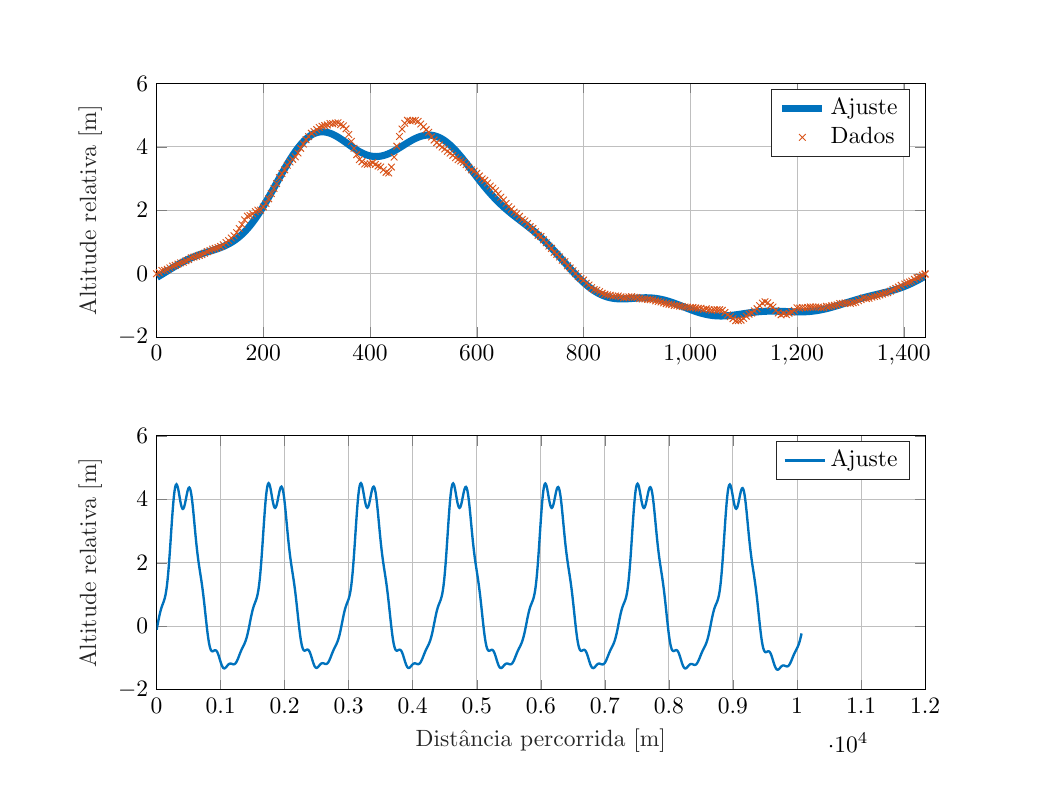
\begin{tikzpicture}[scale=0.85]

\begin{axis}[%
width=4.521in,
height=1.493in,
at={(0.758in,2.554in)},
scale only axis,
xmin=0,
xmax=1440,
ymin=-2,
ymax=6,
ylabel style={font=\color{white!15!black}},
ylabel={Altitude relativa [m]},
axis background/.style={fill=white},
xmajorgrids,
ymajorgrids,
legend style={legend cell align=left, align=left, draw=white!15!black}
]
\addplot [color=mycolor1, line width=3.0pt]
  table[row sep=crcr]{%
1	-0.109711917352081\\
2	-0.0997651899252466\\
3	-0.0897698810709357\\
4	-0.0797287446201807\\
5	-0.0696445893482892\\
6	-0.0595202761884084\\
7	-0.0493587153657857\\
8	-0.0391628634552307\\
9	-0.0289357203643766\\
10	-0.0186803262454241\\
11	-0.00839975833814072\\
12	0.00190287225302775\\
13	0.0122244238447967\\
14	0.0225617275208154\\
15	0.0329115905342793\\
16	0.0432707997642147\\
17	0.0536361252221968\\
18	0.0640043236061954\\
19	0.0743721418981765\\
20	0.0847363210020255\\
21	0.0950935994183011\\
22	0.10544071695227\\
23	0.115774418451625\\
24	0.126091457570232\\
25	0.136388600554215\\
26	0.146662630046643\\
27	0.156910348907032\\
28	0.167128584041869\\
29	0.177314190242296\\
30	0.187464054025096\\
31	0.197575097473076\\
32	0.207644282070944\\
33	0.217668612532733\\
34	0.227645140616833\\
35	0.237570968924681\\
36	0.247443254679135\\
37	0.257259213478585\\
38	0.267016123022827\\
39	0.276711326806761\\
40	0.286342237777955\\
41	0.295906341954157\\
42	0.305401201996829\\
43	0.31482446073683\\
44	0.324173844648373\\
45	0.333447167267411\\
46	0.342642332550677\\
47	0.351757338171582\\
48	0.360790278749266\\
49	0.369739349007116\\
50	0.378602846857121\\
51	0.387379176406482\\
52	0.396066850882955\\
53	0.404664495475469\\
54	0.413170850086601\\
55	0.421584771993597\\
56	0.429905238414653\\
57	0.438131348977282\\
58	0.446262328085635\\
59	0.454297527183765\\
60	0.462236426911864\\
61	0.470078639152616\\
62	0.477823908964901\\
63	0.48547211640215\\
64	0.493023278212789\\
65	0.500477549420268\\
66	0.507835224780295\\
67	0.515096740113001\\
68	0.522262673507857\\
69	0.529333746399276\\
70	0.536310824510952\\
71	0.543194918667103\\
72	0.549987185468885\\
73	0.556688927834383\\
74	0.563301595400693\\
75	0.569826784786738\\
76	0.576266239715584\\
77	0.582621850995138\\
78	0.588895656356266\\
79	0.595089840147451\\
80	0.601206732885304\\
81	0.607248810660309\\
82	0.613218694397363\\
83	0.619119148970783\\
84	0.624953082173597\\
85	0.630723543541058\\
86	0.636433723028484\\
87	0.642086949543627\\
88	0.647686689333937\\
89	0.65323654422923\\
90	0.658740249740376\\
91	0.664201673014787\\
92	0.669624810649624\\
93	0.675013786363756\\
94	0.680372848529662\\
95	0.685706367566601\\
96	0.691018833196505\\
97	0.696314851564177\\
98	0.701599142223534\\
99	0.706876534991757\\
100	0.712151966673313\\
101	0.717430477656014\\
102	0.722717208381324\\
103	0.728017395691319\\
104	0.733336369054802\\
105	0.738679546675193\\
106	0.744052431482965\\
107	0.74946060701548\\
108	0.754909733187238\\
109	0.760405541953632\\
110	0.765953832871438\\
111	0.771560468559376\\
112	0.777231370062181\\
113	0.78297251212174\\
114	0.788789918358932\\
115	0.79468965636995\\
116	0.80067783274093\\
117	0.806760587984841\\
118	0.812944091404689\\
119	0.819234535887123\\
120	0.825638132630689\\
121	0.832161105813\\
122	0.838809687201189\\
123	0.845590110710099\\
124	0.852508606912708\\
125	0.859571397507372\\
126	0.866784689746526\\
127	0.874154670831542\\
128	0.881687502278485\\
129	0.889389314259593\\
130	0.897266199925306\\
131	0.90532420971175\\
132	0.913569345638601\\
133	0.922007555602291\\
134	0.930644727669546\\
135	0.939486684376279\\
136	0.948539177036865\\
137	0.957807880068862\\
138	0.967298385338234\\
139	0.977016196530147\\
140	0.986966723550419\\
141	0.997155276962692\\
142	1.00758706246638\\
143	1.01826717542049\\
144	1.02920059541823\\
145	1.04039218091768\\
146	1.05184666393315\\
147	1.06356864479253\\
148	1.07556258696539\\
149	1.08783281196671\\
150	1.10038349434116\\
151	1.11321865673269\\
152	1.12634216504421\\
153	1.13975772369197\\
154	1.15346887095939\\
155	1.16747897445478\\
156	1.18179122667758\\
157	1.19640864069742\\
158	1.21133404595037\\
159	1.22657008415676\\
160	1.24211920536458\\
161	1.25798366412261\\
162	1.27416551578732\\
163	1.29066661296739\\
164	1.30748860210963\\
165	1.32463292023\\
166	1.34210079179331\\
167	1.35989322574508\\
168	1.37801101269887\\
169	1.39645472228233\\
170	1.41522470064511\\
171	1.43432106813152\\
172	1.45374371712087\\
173	1.47349231003823\\
174	1.49356627753802\\
175	1.51396481686316\\
176	1.53468689038181\\
177	1.55573122430403\\
178	1.57709630758033\\
179	1.59878039098392\\
180	1.62078148637854\\
181	1.64309736617324\\
182	1.66572556296566\\
183	1.68866336937503\\
184	1.71190783806596\\
185	1.73545578196407\\
186	1.75930377466407\\
187	1.78344815103107\\
188	1.80788500799552\\
189	1.83261020554207\\
190	1.85761936789249\\
191	1.88290788488262\\
192	1.90847091353314\\
193	1.93430337981386\\
194	1.96039998060092\\
195	1.98675518582623\\
196	2.01336324081832\\
197	2.04021816883358\\
198	2.06731377377662\\
199	2.09464364310851\\
200	2.12220115094128\\
201	2.14997946131707\\
202	2.17797153167001\\
203	2.20617011646895\\
204	2.23456777103872\\
205	2.26315685555767\\
206	2.29192953922907\\
207	2.3208778046236\\
208	2.34999345219024\\
209	2.37926810493255\\
210	2.40869321324736\\
211	2.43826005992245\\
212	2.46795976528997\\
213	2.49778329253208\\
214	2.52772145313502\\
215	2.55776491248792\\
216	2.58790419562238\\
217	2.6181296930887\\
218	2.6484316669646\\
219	2.67880025699213\\
220	2.70922548683822\\
221	2.73969727047449\\
222	2.77020541867136\\
223	2.80073964560196\\
224	2.83128957555078\\
225	2.86184474972198\\
226	2.89239463314251\\
227	2.92292862165459\\
228	2.95343604899239\\
229	2.98390619393747\\
230	3.01432828754759\\
231	3.04469152045332\\
232	3.07498505021674\\
233	3.10519800874678\\
234	3.13531950976514\\
235	3.16533865631731\\
236	3.19524454832257\\
237	3.2250262901572\\
238	3.25467299826489\\
239	3.28417380878838\\
240	3.31351788521627\\
241	3.34269442603896\\
242	3.37169267240758\\
243	3.40050191578993\\
244	3.42911150561708\\
245	3.45751085691481\\
246	3.48568945791337\\
247	3.51363687762984\\
248	3.54134277341653\\
249	3.5687968984697\\
250	3.59598910929215\\
251	3.62290937310388\\
252	3.64954777519449\\
253	3.6758945262116\\
254	3.70193996937896\\
255	3.7276745876386\\
256	3.75308901071093\\
257	3.77817402206705\\
258	3.80292056580736\\
259	3.82731975344089\\
260	3.85136287055955\\
261	3.87504138340178\\
262	3.8983469453001\\
263	3.92127140300705\\
264	3.94380680289427\\
265	3.96594539701938\\
266	3.98767964905558\\
267	4.00900224007881\\
268	4.02990607420762\\
269	4.05038428409089\\
270	4.07043023623851\\
271	4.09003753619072\\
272	4.10920003352126\\
273	4.12791182667023\\
274	4.14616726760231\\
275	4.16396096628622\\
276	4.18128779499155\\
277	4.19814289239901\\
278	4.21452166752049\\
279	4.23041980342545\\
280	4.24583326077007\\
281	4.26075828112619\\
282	4.27519139010672\\
283	4.28912940028479\\
284	4.30256941390377\\
285	4.31550882537567\\
286	4.32794532356539\\
287	4.33987689385871\\
288	4.35130182001184\\
289	4.36221868578063\\
290	4.37262637632781\\
291	4.38252407940657\\
292	4.39191128631927\\
293	4.40078779264996\\
294	4.40915369876975\\
295	4.41700941011424\\
296	4.4243556372323\\
297	4.43119339560589\\
298	4.43752400524036\\
299	4.44334909002558\\
300	4.44867057686754\\
301	4.45349069459108\\
302	4.457811972614\\
303	4.46163723939335\\
304	4.46496962064464\\
305	4.46781253733511\\
306	4.47016970345218\\
307	4.47204512354857\\
308	4.47344309006565\\
309	4.47436818043676\\
310	4.47482525397249\\
311	4.47481944853005\\
312	4.47435617696902\\
313	4.47344112339597\\
314	4.47208023920066\\
315	4.47027973888656\\
316	4.4680460956988\\
317	4.46538603705261\\
318	4.46230653976574\\
319	4.4588148250982\\
320	4.45491835360308\\
321	4.45062481979224\\
322	4.44594214662091\\
323	4.44087847979514\\
324	4.43544218190666\\
325	4.42964182639929\\
326	4.42348619137163\\
327	4.4169842532207\\
328	4.41014518013129\\
329	4.40297832541612\\
330	4.39549322071171\\
331	4.38769956903536\\
332	4.37960723770841\\
333	4.37122625115138\\
334	4.36256678355636\\
335	4.35363915144245\\
336	4.34445380609995\\
337	4.33502132592912\\
338	4.3253524086795\\
339	4.31545786359578\\
340	4.30534860347637\\
341	4.29503563665075\\
342	4.28453005888202\\
343	4.27384304520075\\
344	4.26298584167675\\
345	4.25196975713493\\
346	4.24080615482196\\
347	4.22950644403014\\
348	4.21808207168501\\
349	4.20654451390342\\
350	4.19490526752858\\
351	4.18317584164875\\
352	4.17136774910629\\
353	4.15949249800367\\
354	4.14756158321321\\
355	4.13558647789713\\
356	4.12357862504465\\
357	4.11154942903283\\
358	4.09951024721769\\
359	4.08747238156232\\
360	4.07544707030866\\
361	4.06344547969927\\
362	4.05147869575584\\
363	4.03955771612091\\
364	4.02769344196904\\
365	4.01589666999407\\
366	4.00417808447856\\
367	3.99254824945187\\
368	3.98101760094286\\
369	3.9695964393335\\
370	3.95829492181928\\
371	3.94712305498246\\
372	3.93609068748393\\
373	3.9252075028795\\
374	3.91448301256626\\
375	3.90392654886448\\
376	3.89354725824066\\
377	3.88335409467688\\
378	3.87335581319173\\
379	3.86356096351794\\
380	3.8539778839416\\
381	3.84461469530785\\
382	3.83547929519766\\
383	3.82657935228032\\
384	3.81792230084603\\
385	3.8095153355228\\
386	3.80136540618183\\
387	3.79347921303529\\
388	3.78586320193033\\
389	3.7785235598429\\
390	3.7714662105749\\
391	3.76469681065797\\
392	3.75822074546703\\
393	3.75204312554657\\
394	3.74616878315244\\
395	3.74060226901177\\
396	3.73534784930355\\
397	3.73040950286191\\
398	3.72579091860443\\
399	3.72149549318722\\
400	3.71752632888846\\
401	3.71388623172202\\
402	3.71057770978239\\
403	3.70760297182218\\
404	3.70496392606295\\
405	3.70266217924036\\
406	3.70069903588404\\
407	3.69907549783257\\
408	3.6977922639839\\
409	3.69684973028098\\
410	3.69624798993257\\
411	3.69598683386881\\
412	3.69606575143087\\
413	3.696483931294\\
414	3.69724026262302\\
415	3.69833333645899\\
416	3.69976144733586\\
417	3.70152259512545\\
418	3.70361448710909\\
419	3.70603454027406\\
420	3.70877988383266\\
421	3.71184736196174\\
422	3.71523353676012\\
423	3.71893469142148\\
424	3.72294683361971\\
425	3.72726569910387\\
426	3.73188675549965\\
427	3.73680520631396\\
428	3.74201599513916\\
429	3.74751381005348\\
430	3.75329308821359\\
431	3.75934802063559\\
432	3.76567255716023\\
433	3.77226041159817\\
434	3.77910506705089\\
435	3.78619978140265\\
436	3.79353759297901\\
437	3.80111132636698\\
438	3.80891359839194\\
439	3.81693682424627\\
440	3.82517322376462\\
441	3.83361482784037\\
442	3.84225348497805\\
443	3.85108086797624\\
444	3.86008848073516\\
445	3.86926766518358\\
446	3.87860960831893\\
447	3.88810534935504\\
448	3.89774578697137\\
449	3.90752168665778\\
450	3.91742368814878\\
451	3.92744231294103\\
452	3.93756797188787\\
453	3.94779097286473\\
454	3.95810152849891\\
455	3.9684897639575\\
456	3.97894572478696\\
457	3.98945938479794\\
458	4.00002065398885\\
459	4.01061938650176\\
460	4.02124538860396\\
461	4.03188842668885\\
462	4.04253823528946\\
463	4.05318452509815\\
464	4.06381699098601\\
465	4.07442532001532\\
466	4.08499919943867\\
467	4.09552832467819\\
468	4.10600240727855\\
469	4.11641118282712\\
470	4.12674441883511\\
471	4.13699192257323\\
472	4.14714354885554\\
473	4.15718920776546\\
474	4.16711887231744\\
475	4.17692258604844\\
476	4.18659047053311\\
477	4.19611273281659\\
478	4.20547967275912\\
479	4.2146816902867\\
480	4.2237092925419\\
481	4.23255310092945\\
482	4.24120385805082\\
483	4.2496524345225\\
484	4.25788983567266\\
485	4.26590720811094\\
486	4.2736958461663\\
487	4.28124719818788\\
488	4.28855287270419\\
489	4.29560464443574\\
490	4.30239446015653\\
491	4.30891444440015\\
492	4.31515690500581\\
493	4.32111433850053\\
494	4.32677943531317\\
495	4.3321450848165\\
496	4.33720438019367\\
497	4.34195062312541\\
498	4.34637732829458\\
499	4.35047822770483\\
500	4.35424727481023\\
501	4.35767864845305\\
502	4.36076675660683\\
503	4.3635062399222\\
504	4.36589197507301\\
505	4.36791907790061\\
506	4.36958290635413\\
507	4.37087906322485\\
508	4.37180339867307\\
509	4.37235201254586\\
510	4.37252125648434\\
511	4.37230773581937\\
512	4.3717083112546\\
513	4.37072010033616\\
514	4.36934047870826\\
515	4.3675670811544\\
516	4.36539780242376\\
517	4.36283079784287\\
518	4.3598644837126\\
519	4.35649753749068\\
520	4.35272889776038\\
521	4.34855776398591\\
522	4.34398359605537\\
523	4.33900611361233\\
524	4.33362529517718\\
525	4.32784137705962\\
526	4.32165485206388\\
527	4.31506646798832\\
528	4.3080772259214\\
529	4.30068837833595\\
530	4.2929014269841\\
531	4.28471812059516\\
532	4.27614045237907\\
533	4.2671706573381\\
534	4.2578112093897\\
535	4.24806481830353\\
536	4.23793442645581\\
537	4.22742320540438\\
538	4.21653455228793\\
539	4.20527208605294\\
540	4.19363964351227\\
541	4.18164127523908\\
542	4.1692812413003\\
543	4.15656400683361\\
544	4.14349423747244\\
545	4.13007679462315\\
546	4.11631673059911\\
547	4.10221928361617\\
548	4.08778987265435\\
549	4.07303409219048\\
550	4.05795770680688\\
551	4.04256664568099\\
552	4.02686699696113\\
553	4.01086500203356\\
554	3.99456704968623\\
555	3.97797967017443\\
556	3.96110952919395\\
557	3.9439634217671\\
558	3.92654826604728\\
559	3.90887109704762\\
560	3.89093906029948\\
561	3.8727594054464\\
562	3.85433947977933\\
563	3.835686721719\\
564	3.81680865425108\\
565	3.7977128783202\\
566	3.77840706618851\\
567	3.75889895476481\\
568	3.73919633891009\\
569	3.71930706472535\\
570	3.69923902282769\\
571	3.6790001416205\\
572	3.65859838056367\\
573	3.63804172344964\\
574	3.61733817169125\\
575	3.59649573762712\\
576	3.57552243785032\\
577	3.55442628656624\\
578	3.53321528898524\\
579	3.51189743475577\\
580	3.49048069144366\\
581	3.46897299806302\\
582	3.44738225866437\\
583	3.42571633598532\\
584	3.40398304516934\\
585	3.38219014755764\\
586	3.36034534455971\\
587	3.33845627160733\\
588	3.31653049219728\\
589	3.29457549202773\\
590	3.27259867323291\\
591	3.25060734872116\\
592	3.22860873662072\\
593	3.20660995483798\\
594	3.18461801573243\\
595	3.1626398209129\\
596	3.14068215615896\\
597	3.11875168647178\\
598	3.09685495125832\\
599	3.07499835965259\\
600	3.05318818597778\\
601	3.03143056535272\\
602	3.00973148944607\\
603	2.98809680238163\\
604	2.96653219679764\\
605	2.94504321006331\\
606	2.92363522065523\\
607	2.90231344469643\\
608	2.88108293266053\\
609	2.85994856624337\\
610	2.83891505540443\\
611	2.81798693557988\\
612	2.7971685650694\\
613	2.77646412259824\\
614	2.75587760505637\\
615	2.73541282541585\\
616	2.71507341082784\\
617	2.69486280090027\\
618	2.67478424615707\\
619	2.65484080667973\\
620	2.63503535093172\\
621	2.61537055476623\\
622	2.59584890061747\\
623	2.57647267687554\\
624	2.55724397744495\\
625	2.53816470148625\\
626	2.5192365533407\\
627	2.50046104263711\\
628	2.48183948458024\\
629	2.46337300041987\\
630	2.44506251809937\\
631	2.42690877308266\\
632	2.40891230935803\\
633	2.39107348061748\\
634	2.37339245160964\\
635	2.35586919966461\\
636	2.33850351638863\\
637	2.32129500952646\\
638	2.30424310498911\\
639	2.28734704904458\\
640	2.27060591066894\\
641	2.25401858405504\\
642	2.23758379127608\\
643	2.22130008510087\\
644	2.20516585195784\\
645	2.18917931504444\\
646	2.17333853757858\\
647	2.15764142618867\\
648	2.1420857344385\\
649	2.12666906648345\\
650	2.11138888085396\\
651	2.09624249436254\\
652	2.08122708613009\\
653	2.06633970172749\\
654	2.05157725742822\\
655	2.03693654456761\\
656	2.02241423400436\\
657	2.0080068806799\\
658	1.9937109282708\\
659	1.97952271392983\\
660	1.9654384731108\\
661	1.95145434447245\\
662	1.93756637485646\\
663	1.92377052433487\\
664	1.91006267132177\\
665	1.89643861774434\\
666	1.88289409426817\\
667	1.86942476557189\\
668	1.85602623566586\\
669	1.84269405324981\\
670	1.82942371710442\\
671	1.81621068151138\\
672	1.80305036169709\\
673	1.78993813929447\\
674	1.77686936781789\\
675	1.7638393781459\\
676	1.75084348400672\\
677	1.73787698746101\\
678	1.72493518437715\\
679	1.71201336989347\\
680	1.69910684386258\\
681	1.68621091627265\\
682	1.67332091264045\\
683	1.66043217937128\\
684	1.6475400890807\\
685	1.6346400458732\\
686	1.62172749057283\\
687	1.6087979059011\\
688	1.59584682159725\\
689	1.58286981947622\\
690	1.56986253841976\\
691	1.55682067929601\\
692	1.54374000980317\\
693	1.53061636923277\\
694	1.51744567314825\\
695	1.50422391797463\\
696	1.49094718549518\\
697	1.47761164725092\\
698	1.46421356883914\\
699	1.45074931410699\\
700	1.43721534923656\\
701	1.42360824671759\\
702	1.40992468920459\\
703	1.3961614732547\\
704	1.38231551294322\\
705	1.36838384335348\\
706	1.35436362393823\\
707	1.34025214174942\\
708	1.32604681453375\\
709	1.31174519369124\\
710	1.29734496709447\\
711	1.28284396176586\\
712	1.268240146411\\
713	1.25353163380579\\
714	1.23871668303546\\
715	1.22379370158368\\
716	1.20876124727001\\
717	1.19361803003431\\
718	1.17836291356657\\
719	1.16299491678098\\
720	1.1475132151332\\
721	1.13191714177985\\
722	1.11620618857945\\
723	1.10038000693407\\
724	1.08443840847141\\
725	1.06838136556677\\
726	1.05220901170479\\
727	1.03592164168099\\
728	1.01951971164311\\
729	1.00300383897255\\
730	0.986374802006352\\
731	0.969633539600276\\
732	0.952781150533595\\
733	0.935818892756565\\
734	0.918748182481501\\
735	0.901570593118622\\
736	0.884287854057938\\
737	0.866901849298617\\
738	0.849414615927377\\
739	0.831828342447627\\
740	0.814145366961175\\
741	0.796368175204486\\
742	0.778499398441604\\
743	0.760541811215943\\
744	0.742498328963352\\
745	0.724372005488898\\
746	0.706166030310012\\
747	0.687883725868709\\
748	0.669528544615737\\
749	0.651104065969613\\
750	0.632613993153629\\
751	0.614062149913995\\
752	0.59545247712242\\
753	0.576789029266517\\
754	0.558075970831511\\
755	0.539317572576848\\
756	0.52051820771137\\
757	0.501682347970819\\
758	0.482814559601524\\
759	0.463919499254195\\
760	0.445001909791833\\
761	0.426066616015826\\
762	0.40711852031439\\
763	0.388162598237564\\
764	0.369203894003033\\
765	0.3502475159371\\
766	0.331298631855219\\
767	0.31236246438649\\
768	0.293444286246612\\
769	0.274549415463817\\
770	0.255683210562321\\
771	0.236851065707892\\
772	0.218058405820147\\
773	0.199310681656212\\
774	0.1806133648704\\
775	0.161971943054579\\
776	0.143391914763913\\
777	0.124878784532656\\
778	0.106438057884686\\
779	0.0880752363434726\\
780	0.0697958124461434\\
781	0.051605264766321\\
782	0.0335090529503783\\
783	0.0155126127717403\\
784	-0.00237864879216312\\
785	-0.0201593584557181\\
786	-0.0378241814891784\\
787	-0.0553678265464439\\
788	-0.0727850504521007\\
789	-0.0900706629433051\\
790	-0.107219531362142\\
791	-0.124226585294145\\
792	-0.14108682114871\\
793	-0.157795306677225\\
794	-0.174347185424754\\
795	-0.190737681111248\\
796	-0.206962101938258\\
797	-0.223015844817255\\
798	-0.238894399515718\\
799	-0.254593352717232\\
800	-0.270108391991932\\
801	-0.28543530967372\\
802	-0.300570006640766\\
803	-0.315508495995898\\
804	-0.330246906643611\\
805	-0.344781486760483\\
806	-0.359108607155931\\
807	-0.373224764520321\\
808	-0.387126584557567\\
809	-0.400810824999471\\
810	-0.414274378499148\\
811	-0.427514275401029\\
812	-0.440527686385026\\
813	-0.453311924982577\\
814	-0.465864449962419\\
815	-0.478182867584034\\
816	-0.490264933716879\\
817	-0.502108555823604\\
818	-0.513711794805605\\
819	-0.525072866709402\\
820	-0.536190144292439\\
821	-0.547062158447048\\
822	-0.557687599481469\\
823	-0.568065318256914\\
824	-0.578194327179846\\
825	-0.588073801048726\\
826	-0.597703077754682\\
827	-0.607081658835615\\
828	-0.616209209883474\\
829	-0.625085560804492\\
830	-0.633710705932377\\
831	-0.642084803994541\\
832	-0.650208177931617\\
833	-0.658081314570625\\
834	-0.665704864152313\\
835	-0.673079639713301\\
836	-0.680206616323806\\
837	-0.687086930181876\\
838	-0.693721877565144\\
839	-0.7001129136413\\
840	-0.706261651138562\\
841	-0.712169858877593\\
842	-0.717839460166397\\
843	-0.723272531059889\\
844	-0.728471298485927\\
845	-0.733438138239738\\
846	-0.738175572848777\\
847	-0.74268626931016\\
848	-0.746973036702966\\
849	-0.75103882367777\\
850	-0.754886715825915\\
851	-0.758519932931108\\
852	-0.761941826106057\\
853	-0.765155874816942\\
854	-0.76816568379864\\
855	-0.770974979863685\\
856	-0.773587608608072\\
857	-0.776007531017083\\
858	-0.778238819974403\\
859	-0.780285656677883\\
860	-0.782152326965385\\
861	-0.783843217554211\\
862	-0.785362812197718\\
863	-0.786715687762759\\
864	-0.787906510231672\\
865	-0.788940030632617\\
866	-0.789821080902082\\
867	-0.790554569683474\\
868	-0.791145478065743\\
869	-0.791598855266032\\
870	-0.791919814260404\\
871	-0.792113527366725\\
872	-0.792185221783824\\
873	-0.79214017509109\\
874	-0.791983710712676\\
875	-0.791721193350526\\
876	-0.791358024390446\\
877	-0.790899637285467\\
878	-0.790351492920757\\
879	-0.789719074964342\\
880	-0.789007885207913\\
881	-0.788223438901982\\
882	-0.787371260089664\\
883	-0.786456876943336\\
884	-0.785485817108429\\
885	-0.784463603058585\\
886	-0.783395747466388\\
887	-0.782287748593872\\
888	-0.781145085706961\\
889	-0.779973214517981\\
890	-0.778777562660339\\
891	-0.777563525199437\\
892	-0.776336460183834\\
893	-0.775101684240631\\
894	-0.773864468219008\\
895	-0.772630032885777\\
896	-0.771403544676772\\
897	-0.770190111507825\\
898	-0.768994778649033\\
899	-0.767822524665918\\
900	-0.766678257431061\\
901	-0.765566810209672\\
902	-0.764492937822513\\
903	-0.763461312889499\\
904	-0.762476522157216\\
905	-0.761543062913525\\
906	-0.76066533949231\\
907	-0.759847659871367\\
908	-0.759094232366312\\
909	-0.758409162423294\\
910	-0.757796449513224\\
911	-0.757259984130101\\
912	-0.756803544895926\\
913	-0.756430795774596\\
914	-0.75614528339705\\
915	-0.755950434499845\\
916	-0.755849553479214\\
917	-0.755845820062558\\
918	-0.755942287099205\\
919	-0.756141878472153\\
920	-0.756447387132398\\
921	-0.756861473257333\\
922	-0.757386662534574\\
923	-0.758025344572475\\
924	-0.758779771438427\\
925	-0.759652056325972\\
926	-0.760644172351588\\
927	-0.761757951481908\\
928	-0.762995083592008\\
929	-0.764357115655263\\
930	-0.765845451065164\\
931	-0.767461349089345\\
932	-0.769205924455963\\
933	-0.771080147072435\\
934	-0.773084841876425\\
935	-0.775220688818839\\
936	-0.77748822297847\\
937	-0.779887834807809\\
938	-0.782419770509426\\
939	-0.785084132542182\\
940	-0.787880880256441\\
941	-0.790809830657308\\
942	-0.793870659294824\\
943	-0.797062901279904\\
944	-0.800385952424716\\
945	-0.803839070506079\\
946	-0.807421376650327\\
947	-0.811131856838005\\
948	-0.81496936352663\\
949	-0.81893261738966\\
950	-0.8230202091697\\
951	-0.827230601643877\\
952	-0.83156213169921\\
953	-0.836013012515704\\
954	-0.840581335854816\\
955	-0.845265074450822\\
956	-0.850062084502543\\
957	-0.85497010826279\\
958	-0.85998677672282\\
959	-0.865109612388973\\
960	-0.870336032148637\\
961	-0.875663350222557\\
962	-0.881088781200466\\
963	-0.886609443156927\\
964	-0.892222360844222\\
965	-0.897924468959036\\
966	-0.903712615479655\\
967	-0.909583565070312\\
968	-0.915534002549265\\
969	-0.921560536417165\\
970	-0.927659702442173\\
971	-0.933827967298308\\
972	-0.940061732253399\\
973	-0.946357336903024\\
974	-0.952711062946772\\
975	-0.959119138003116\\
976	-0.965577739459196\\
977	-0.972082998351742\\
978	-0.978631003275387\\
979	-0.98521780431458\\
980	-0.991839416995314\\
981	-0.998491826252851\\
982	-1.00517099041166\\
983	-1.01187284517371\\
984	-1.01859330761144\\
985	-1.02532828016136\\
986	-1.0320736546148\\
987	-1.03882531610179\\
988	-1.04557914706442\\
989	-1.05233103121591\\
990	-1.05907685748172\\
991	-1.06581252391888\\
992	-1.07253394161012\\
993	-1.07923703852889\\
994	-1.08591776337192\\
995	-1.09257208935567\\
996	-1.09919601797318\\
997	-1.10578558270782\\
998	-1.11233685270072\\
999	-1.1188459363683\\
1000	-1.12530898496673\\
1001	-1.13172219610016\\
1002	-1.13808181716937\\
1003	-1.1443841487579\\
1004	-1.15062554795259\\
1005	-1.15680243159548\\
1006	-1.16291127946437\\
1007	-1.16894863737899\\
1008	-1.1749111202303\\
1009	-1.18079541493006\\
1010	-1.18659828327827\\
1011	-1.19231656474594\\
1012	-1.19794717917071\\
1013	-1.20348712936323\\
1014	-1.2089335036219\\
1015	-1.21428347815398\\
1016	-1.219534319401\\
1017	-1.2246833862666\\
1018	-1.22972813224493\\
1019	-1.23466610744795\\
1020	-1.23949496052998\\
1021	-1.24421244050807\\
1022	-1.24881639847666\\
1023	-1.25330478921534\\
1024	-1.25767567268853\\
1025	-1.26192721543589\\
1026	-1.26605769185266\\
1027	-1.27006548535891\\
1028	-1.27394908945704\\
1029	-1.2777071086769\\
1030	-1.28133825940791\\
1031	-1.28484137061795\\
1032	-1.28821538445846\\
1033	-1.29145935675581\\
1034	-1.29457245738869\\
1035	-1.29755397055166\\
1036	-1.30040329490486\\
1037	-1.30311994361034\\
1038	-1.30570354425522\\
1039	-1.30815383866212\\
1040	-1.31047068258767\\
1041	-1.31265404530945\\
1042	-1.31470400910254\\
1043	-1.31662076860622\\
1044	-1.31840463008209\\
1045	-1.32005601056461\\
1046	-1.32157543690528\\
1047	-1.32296354471177\\
1048	-1.32422107718351\\
1049	-1.32534888384507\\
1050	-1.32634791917912\\
1051	-1.32721924116057\\
1052	-1.32796400969371\\
1053	-1.32858348495424\\
1054	-1.32907902563818\\
1055	-1.32945208711966\\
1056	-1.32970421951983\\
1057	-1.32983706568903\\
1058	-1.32985235910456\\
1059	-1.32975192168643\\
1060	-1.32953766153355\\
1061	-1.32921157058291\\
1062	-1.32877572219428\\
1063	-1.32823226866313\\
1064	-1.32758343866457\\
1065	-1.32683153463096\\
1066	-1.32597893006612\\
1067	-1.32502806679908\\
1068	-1.32398145218017\\
1069	-1.32284165622264\\
1070	-1.32161130869272\\
1071	-1.32029309615128\\
1072	-1.31888975895017\\
1073	-1.31740408818645\\
1074	-1.31583892261768\\
1075	-1.31419714554153\\
1076	-1.31248168164289\\
1077	-1.31069549381186\\
1078	-1.30884157993587\\
1079	-1.30692296966921\\
1080	-1.30494272118333\\
1081	-1.30290391790131\\
1082	-1.30080966521972\\
1083	-1.29866308722129\\
1084	-1.29646732338178\\
1085	-1.29422552527429\\
1086	-1.2919408532744\\
1087	-1.28961647326955\\
1088	-1.28725555337581\\
1089	-1.28486126066543\\
1090	-1.2824367579085\\
1091	-1.27998520033189\\
1092	-1.27750973239868\\
1093	-1.27501348461138\\
1094	-1.27249957034204\\
1095	-1.2699710826924\\
1096	-1.2674310913871\\
1097	-1.2648826397032\\
1098	-1.26232874143874\\
1099	-1.2597723779235\\
1100	-1.25721649507488\\
1101	-1.25466400050152\\
1102	-1.2521177606578\\
1103	-1.24958059805166\\
1104	-1.24705528850855\\
1105	-1.24454455849423\\
1106	-1.24205108249869\\
1107	-1.23957748048393\\
1108	-1.23712631539793\\
1109	-1.23470009075705\\
1110	-1.23230124829924\\
1111	-1.22993216571023\\
1112	-1.22759515442466\\
1113	-1.22529245750443\\
1114	-1.22302624759592\\
1115	-1.22079862496816\\
1116	-1.21861161563352\\
1117	-1.21646716955283\\
1118	-1.21436715892627\\
1119	-1.21231337657165\\
1120	-1.21030753439152\\
1121	-1.20835126193031\\
1122	-1.20644610502275\\
1123	-1.20459352453476\\
1124	-1.20279489519767\\
1125	-1.2010515045369\\
1126	-1.19936455189564\\
1127	-1.1977351475546\\
1128	-1.19616431194811\\
1129	-1.19465297497731\\
1130	-1.19320197542079\\
1131	-1.19181206044295\\
1132	-1.1904838852004\\
1133	-1.18921801254635\\
1134	-1.18801491283324\\
1135	-1.18687496381329\\
1136	-1.18579845063693\\
1137	-1.18478556594874\\
1138	-1.18383641008061\\
1139	-1.18295099134154\\
1140	-1.18212922640351\\
1141	-1.18137094078277\\
1142	-1.18067586941579\\
1143	-1.18004365732892\\
1144	-1.17947386040085\\
1145	-1.17896594621674\\
1146	-1.17851929501302\\
1147	-1.17813320071137\\
1148	-1.17780687204073\\
1149	-1.1775394337459\\
1150	-1.17732992788112\\
1151	-1.17717731518708\\
1152	-1.1770804765497\\
1153	-1.17703821453898\\
1154	-1.17704925502587\\
1155	-1.17711224887545\\
1156	-1.1772257737144\\
1157	-1.17738833577052\\
1158	-1.17759837178243\\
1159	-1.17785425097697\\
1160	-1.17815427711228\\
1161	-1.17849669058402\\
1162	-1.17887967059248\\
1163	-1.17930133736801\\
1164	-1.17975975445233\\
1165	-1.1802529310332\\
1166	-1.18077882432967\\
1167	-1.18133534202543\\
1168	-1.18192034474745\\
1169	-1.18253164858717\\
1170	-1.18316702766148\\
1171	-1.18382421671065\\
1172	-1.18450091373035\\
1173	-1.18519478263486\\
1174	-1.18590345594859\\
1175	-1.18662453752291\\
1176	-1.18735560527541\\
1177	-1.18809421394852\\
1178	-1.18883789788457\\
1179	-1.18958417381426\\
1180	-1.19033054365544\\
1181	-1.19107449731941\\
1182	-1.1918135155214\\
1183	-1.19254507259247\\
1184	-1.19326663928973\\
1185	-1.19397568560175\\
1186	-1.19466968354636\\
1187	-1.19534610995774\\
1188	-1.19600244925976\\
1189	-1.19663619622282\\
1190	-1.19724485870104\\
1191	-1.19782596034705\\
1192	-1.19837704330142\\
1193	-1.19889567085392\\
1194	-1.19937943007381\\
1195	-1.19982593440633\\
1196	-1.20023282623274\\
1197	-1.20059777939114\\
1198	-1.20091850165549\\
1199	-1.20119273717016\\
1200	-1.20141826883758\\
1201	-1.20159292065635\\
1202	-1.20171456000747\\
1203	-1.20178109988638\\
1204	-1.20179050107823\\
1205	-1.20174077427449\\
1206	-1.20162998212844\\
1207	-1.20145624124744\\
1208	-1.20121772412017\\
1209	-1.20091266097655\\
1210	-1.20053934157862\\
1211	-1.20009611694053\\
1212	-1.19958140097587\\
1213	-1.19899367207067\\
1214	-1.19833147458047\\
1215	-1.19759342025004\\
1216	-1.19677818955417\\
1217	-1.19588453295834\\
1218	-1.19491127209801\\
1219	-1.19385730087528\\
1220	-1.1927215864719\\
1221	-1.19150317027772\\
1222	-1.19020116873358\\
1223	-1.18881477408792\\
1224	-1.18734325506641\\
1225	-1.18578595745393\\
1226	-1.18414230458845\\
1227	-1.18241179776642\\
1228	-1.18059401655926\\
1229	-1.17868861904075\\
1230	-1.17669534192531\\
1231	-1.17461400061693\\
1232	-1.17244448916898\\
1233	-1.170186780155\\
1234	-1.16784092445076\\
1235	-1.16540705092781\\
1236	-1.16288536605916\\
1237	-1.16027615343751\\
1238	-1.15757977320668\\
1239	-1.15479666140695\\
1240	-1.15192732923521\\
1241	-1.14897236222076\\
1242	-1.14593241931773\\
1243	-1.14280823191534\\
1244	-1.13960060276704\\
1245	-1.13631040483988\\
1246	-1.13293858008542\\
1247	-1.1294861381337\\
1248	-1.12595415491162\\
1249	-1.12234377118752\\
1250	-1.11865619104356\\
1251	-1.11489268027755\\
1252	-1.1110545647363\\
1253	-1.10714322858218\\
1254	-1.10316011249499\\
1255	-1.0991067118111\\
1256	-1.09498457460212\\
1257	-1.09079529969509\\
1258	-1.0865405346366\\
1259	-1.08222197360304\\
1260	-1.07784135525943\\
1261	-1.07340046056913\\
1262	-1.06890111055705\\
1263	-1.06434516402874\\
1264	-1.05973451524807\\
1265	-1.05507109157593\\
1266	-1.05035685107288\\
1267	-1.04559378006813\\
1268	-1.04078389069783\\
1269	-1.03592921841534\\
1270	-1.0310318194763\\
1271	-1.02609376840127\\
1272	-1.0211171554189\\
1273	-1.01610408389239\\
1274	-1.01105666773226\\
1275	-1.00597702879816\\
1276	-1.00086729429286\\
1277	-0.99572959415116\\
1278	-0.990566058426787\\
1279	-0.98537881468013\\
1280	-0.980169985369829\\
1281	-0.974941685251106\\
1282	-0.969696018783796\\
1283	-0.964435077552992\\
1284	-0.959160937705216\\
1285	-0.953875657403025\\
1286	-0.948581274300908\\
1287	-0.943279803045356\\
1288	-0.937973232801914\\
1289	-0.932663524812038\\
1290	-0.927352609982524\\
1291	-0.922042386510245\\
1292	-0.916734717544915\\
1293	-0.911431428892525\\
1294	-0.906134306762095\\
1295	-0.900845095558306\\
1296	-0.895565495722543\\
1297	-0.890297161624842\\
1298	-0.885041699509146\\
1299	-0.879800665494259\\
1300	-0.874575563632802\\
1301	-0.869367844030426\\
1302	-0.864178901027459\\
1303	-0.859010071445129\\
1304	-0.853862632898394\\
1305	-0.848737802177382\\
1306	-0.843636733699336\\
1307	-0.838560518032916\\
1308	-0.833510180496597\\
1309	-0.828486679832866\\
1310	-0.8234909069598\\
1311	-0.818523683801552\\
1312	-0.813585762199177\\
1313	-0.808677822903139\\
1314	-0.80380047464877\\
1315	-0.798954253315844\\
1316	-0.794139621173347\\
1317	-0.78935696621044\\
1318	-0.784606601554505\\
1319	-0.779888764977077\\
1320	-0.775203618488375\\
1321	-0.770551248021045\\
1322	-0.76593166320362\\
1323	-0.761344797224135\\
1324	-0.756790506784199\\
1325	-0.752268572143764\\
1326	-0.747778697256699\\
1327	-0.743320509997206\\
1328	-0.738893562477005\\
1329	-0.734497331453102\\
1330	-0.730131218825878\\
1331	-0.725794552227129\\
1332	-0.721486585697577\\
1333	-0.71720650045329\\
1334	-0.71295340574034\\
1335	-0.708726339776931\\
1336	-0.704524270782146\\
1337	-0.700346098090333\\
1338	-0.696190653350103\\
1339	-0.69205670180676\\
1340	-0.687942943666946\\
1341	-0.683848015544151\\
1342	-0.679770491983664\\
1343	-0.67570888706545\\
1344	-0.671661656083346\\
1345	-0.667627197298887\\
1346	-0.663603853767973\\
1347	-0.659589915238527\\
1348	-0.655583620117199\\
1349	-0.651583157503078\\
1350	-0.647586669286329\\
1351	-0.643592252309563\\
1352	-0.639597960589686\\
1353	-0.635601807597915\\
1354	-0.631601768595552\\
1355	-0.627595783023065\\
1356	-0.62358175693994\\
1357	-0.619557565512724\\
1358	-0.615521055548607\\
1359	-0.611470048071829\\
1360	-0.60740234094017\\
1361	-0.603315711498686\\
1362	-0.599207919267859\\
1363	-0.595076708663225\\
1364	-0.590919811743553\\
1365	-0.586734950984565\\
1366	-0.582519842075192\\
1367	-0.578272196733286\\
1368	-0.573989725537698\\
1369	-0.569670140773615\\
1370	-0.565311159287994\\
1371	-0.560910505351947\\
1372	-0.556465913526868\\
1373	-0.551975131531127\\
1374	-0.547435923104105\\
1375	-0.542846070864365\\
1376	-0.538203379158715\\
1377	-0.533505676898963\\
1378	-0.528750820383126\\
1379	-0.523936696097869\\
1380	-0.519061223498992\\
1381	-0.514122357766729\\
1382	-0.509118092532717\\
1383	-0.504046462575438\\
1384	-0.49890554648102\\
1385	-0.493693469266257\\
1386	-0.488408404960779\\
1387	-0.483048579145316\\
1388	-0.477612271443018\\
1389	-0.47209781796087\\
1390	-0.46650361367826\\
1391	-0.460828114779785\\
1392	-0.45506984092948\\
1393	-0.449227377483646\\
1394	-0.443299377639554\\
1395	-0.437284564517328\\
1396	-0.4311817331724\\
1397	-0.424989752535953\\
1398	-0.418707567280881\\
1399	-0.412334199610824\\
1400	-0.405868750969924\\
1401	-0.399310403671038\\
1402	-0.392658422440181\\
1403	-0.385912155875092\\
1404	-0.379071037815874\\
1405	-0.372134588625751\\
1406	-0.365102416380069\\
1407	-0.357974217961757\\
1408	-0.350749780061564\\
1409	-0.343428980081461\\
1410	-0.336011786939708\\
1411	-0.328498261776184\\
1412	-0.320888558556666\\
1413	-0.313182924574844\\
1414	-0.305381700850977\\
1415	-0.297485322426174\\
1416	-0.289494318551407\\
1417	-0.281409312770474\\
1418	-0.273231022896199\\
1419	-0.264960260879327\\
1420	-0.256597932569617\\
1421	-0.248145037368798\\
1422	-0.239602667775124\\
1423	-0.23097200881941\\
1424	-0.222254337392517\\
1425	-0.213451021464379\\
1426	-0.204563519194781\\
1427	-0.195593377936197\\
1428	-0.186542233129126\\
1429	-0.177411807090472\\
1430	-0.168203907695618\\
1431	-0.158920426954973\\
1432	-0.149563339485869\\
1433	-0.140134700880815\\
1434	-0.130636645973205\\
1435	-0.121071387001703\\
1436	-0.111441211674644\\
1437	-0.101748481135875\\
1438	-0.0919956278335936\\
1439	-0.0821851532938451\\
1440	-0.0723196258004223\\
};
\addlegendentry{Ajuste}

\addplot [color=mycolor2, only marks, mark=x, mark options={solid, mycolor2}]
  table[row sep=crcr]{%
0	0\\
5.1222	0.035738\\
10.052	0.10497\\
15.102	0.10772\\
20.056	0.14341\\
25.018	0.18539\\
30.099	0.24281\\
35.019	0.26534\\
40.103	0.30621\\
45.03	0.34432\\
50.02	0.36324\\
55.06	0.4084\\
60.082	0.44874\\
65.003	0.50745\\
70.013	0.52866\\
75.043	0.54874\\
80.029	0.58008\\
85.054	0.60309\\
90.004	0.64756\\
95.034	0.69913\\
100.08	0.73437\\
105.09	0.77665\\
110.03	0.80147\\
115.11	0.8308\\
120.05	0.85947\\
125.08	0.91471\\
130.04	0.987\\
135.06	1.0446\\
140.02	1.1265\\
145.07	1.1976\\
150.07	1.2977\\
155.07	1.4261\\
160.05	1.5534\\
165.02	1.7003\\
170.06	1.8176\\
175.03	1.8384\\
180.1	1.8899\\
185.09	1.959\\
190.08	2.0057\\
195.07	2.0065\\
200.08	2.1076\\
205.05	2.2171\\
210.04	2.3643\\
215.1	2.5291\\
220.07	2.6873\\
225.1	2.8419\\
230.05	3.0317\\
235.08	3.1583\\
240.02	3.2784\\
245.01	3.4202\\
250.02	3.5219\\
255.05	3.6083\\
260.01	3.6875\\
265	3.8082\\
270.07	3.9549\\
275.02	4.0884\\
280.08	4.2276\\
285.07	4.3234\\
290.09	4.4291\\
295.02	4.4829\\
300.06	4.5449\\
305.07	4.61\\
310.07	4.648\\
315.05	4.6728\\
320.01	4.6917\\
325.05	4.7362\\
330.01	4.7312\\
335.08	4.7492\\
340.01	4.7603\\
345.05	4.7026\\
350.06	4.6628\\
355.04	4.5688\\
360.09	4.3908\\
365.05	4.1747\\
370.01	3.9563\\
375.05	3.7561\\
380.01	3.5984\\
385.01	3.5353\\
390.02	3.4615\\
395.07	3.4505\\
400.1	3.4657\\
405.04	3.5032\\
410.05	3.4511\\
415	3.3952\\
420.07	3.3656\\
425.01	3.2732\\
430.02	3.1978\\
435.03	3.1787\\
440.06	3.3637\\
445.07	3.6768\\
450.11	4.0237\\
455.11	4.3273\\
460.03	4.5621\\
465.01	4.7456\\
470.09	4.8381\\
475.01	4.8199\\
480.09	4.8295\\
485	4.8346\\
490.09	4.8057\\
495.09	4.7223\\
500.09	4.6332\\
505.1	4.5413\\
510.02	4.4621\\
515.05	4.3114\\
520.05	4.2162\\
525.01	4.134\\
530.04	4.0624\\
535.01	3.9909\\
540	3.9346\\
545.08	3.8595\\
550.12	3.8051\\
555.1	3.7335\\
560.09	3.6563\\
565.02	3.599\\
570.06	3.5572\\
575.09	3.5131\\
580.08	3.4391\\
585	3.3567\\
590.01	3.2757\\
595.05	3.2379\\
600.02	3.1674\\
605.08	3.0848\\
610.02	2.9922\\
615	2.9465\\
620.02	2.8593\\
625.11	2.7651\\
630.08	2.6997\\
635.08	2.6199\\
640.02	2.5204\\
645.04	2.4145\\
650.07	2.3246\\
655	2.2181\\
660.06	2.1146\\
665.02	2.038\\
670.06	1.9449\\
675.05	1.8925\\
680.09	1.8092\\
685.08	1.709\\
690.04	1.6652\\
695.04	1.5816\\
700.02	1.4836\\
705.1	1.4271\\
710.02	1.3237\\
715	1.2147\\
720.11	1.1747\\
725.08	1.0693\\
730.02	0.9783\\
735.02	0.87326\\
740.01	0.80079\\
745.06	0.67547\\
750.09	0.61633\\
755.06	0.53173\\
760.08	0.42591\\
765	0.38467\\
770.1	0.25097\\
775.04	0.185\\
780.1	0.094467\\
785.11	0.0042468\\
790.01	-0.087749\\
795.03	-0.15127\\
800.04	-0.19791\\
805.06	-0.29861\\
810.07	-0.35415\\
815.01	-0.43642\\
820.07	-0.50071\\
825.05	-0.5167\\
830.08	-0.56259\\
835.08	-0.6105\\
840.01	-0.64431\\
845.08	-0.66497\\
850.11	-0.67766\\
855.07	-0.70386\\
860.02	-0.69959\\
865.1	-0.70008\\
870.02	-0.72612\\
875.09	-0.75503\\
880.11	-0.74512\\
885.04	-0.72702\\
890.06	-0.72219\\
895.01	-0.74177\\
900.04	-0.74645\\
905.09	-0.78183\\
910.06	-0.79228\\
915.01	-0.79059\\
920.11	-0.80498\\
925	-0.81388\\
930.09	-0.82108\\
935.08	-0.85434\\
940.08	-0.87037\\
945.02	-0.8898\\
950.11	-0.91711\\
955	-0.941\\
960.02	-0.95908\\
965.01	-0.97259\\
970.07	-0.9977\\
975.02	-1.0021\\
980.02	-1.0205\\
985.06	-1.03\\
990.07	-1.0475\\
995.09	-1.0488\\
1000.1	-1.0607\\
1005	-1.0603\\
1010.1	-1.0762\\
1015	-1.0899\\
1020.1	-1.0865\\
1025	-1.1233\\
1030	-1.1057\\
1035.1	-1.1309\\
1040.1	-1.1516\\
1045.1	-1.1333\\
1050.1	-1.1306\\
1055	-1.1343\\
1060.1	-1.1496\\
1065	-1.2185\\
1070.1	-1.294\\
1075.1	-1.3496\\
1080.1	-1.4133\\
1085.1	-1.4789\\
1090.1	-1.4778\\
1095.1	-1.4619\\
1100	-1.4065\\
1105	-1.3362\\
1110.1	-1.2712\\
1115.1	-1.2374\\
1120.1	-1.1685\\
1125.1	-1.0986\\
1130	-1.0041\\
1135	-0.92332\\
1140	-0.88023\\
1145.1	-0.91493\\
1150.1	-0.9995\\
1155	-1.0491\\
1160.1	-1.1572\\
1165	-1.2352\\
1170.1	-1.2925\\
1175	-1.2543\\
1180.1	-1.2889\\
1185.1	-1.2424\\
1190.1	-1.2007\\
1195	-1.1524\\
1200.1	-1.0711\\
1205	-1.0818\\
1210	-1.0683\\
1215.1	-1.0743\\
1220	-1.0607\\
1225	-1.0466\\
1230.1	-1.0469\\
1235.1	-1.049\\
1240	-1.0506\\
1245	-1.0674\\
1250	-1.0704\\
1255.1	-1.0248\\
1260.1	-1.0326\\
1265	-1.0105\\
1270.1	-0.99422\\
1275	-0.98019\\
1280.1	-0.93839\\
1285	-0.93409\\
1290.1	-0.92035\\
1295.1	-0.9174\\
1300	-0.93492\\
1305.1	-0.91239\\
1310.1	-0.89661\\
1315.1	-0.85047\\
1320.1	-0.81659\\
1325.1	-0.76624\\
1330.1	-0.78241\\
1335	-0.77116\\
1340.1	-0.73442\\
1345.1	-0.71422\\
1350	-0.70423\\
1355	-0.66556\\
1360.1	-0.63987\\
1365.1	-0.60605\\
1370	-0.59789\\
1375	-0.54782\\
1380	-0.49583\\
1385	-0.46034\\
1390	-0.41838\\
1395.1	-0.363\\
1401.9	-0.32049\\
1406.3	-0.28726\\
1410.6	-0.25818\\
1415.1	-0.22964\\
1420	-0.17512\\
1425	-0.12472\\
1430.1	-0.10287\\
1435.1	-0.048184\\
1440	-0.01308\\
1440	0\\
1445.1222	0.035738\\
1450.052	0.10497\\
1455.102	0.10772\\
1460.056	0.14341\\
1465.018	0.18539\\
1470.099	0.24281\\
1475.019	0.26534\\
1480.103	0.30621\\
1485.03	0.34432\\
1490.02	0.36324\\
1495.06	0.4084\\
1500.082	0.44874\\
1505.003	0.50745\\
1510.013	0.52866\\
1515.043	0.54874\\
1520.029	0.58008\\
1525.054	0.60309\\
1530.004	0.64756\\
1535.034	0.69913\\
1540.08	0.73437\\
1545.09	0.77665\\
1550.03	0.80147\\
1555.11	0.8308\\
1560.05	0.85947\\
1565.08	0.91471\\
1570.04	0.987\\
1575.06	1.0446\\
1580.02	1.1265\\
1585.07	1.1976\\
1590.07	1.2977\\
1595.07	1.4261\\
1600.05	1.5534\\
1605.02	1.7003\\
1610.06	1.8176\\
1615.03	1.8384\\
1620.1	1.8899\\
1625.09	1.959\\
1630.08	2.0057\\
1635.07	2.0065\\
1640.08	2.1076\\
1645.05	2.2171\\
1650.04	2.3643\\
1655.1	2.5291\\
1660.07	2.6873\\
1665.1	2.8419\\
1670.05	3.0317\\
1675.08	3.1583\\
1680.02	3.2784\\
1685.01	3.4202\\
1690.02	3.5219\\
1695.05	3.6083\\
1700.01	3.6875\\
1705	3.8082\\
1710.07	3.9549\\
1715.02	4.0884\\
1720.08	4.2276\\
1725.07	4.3234\\
1730.09	4.4291\\
1735.02	4.4829\\
1740.06	4.5449\\
1745.07	4.61\\
1750.07	4.648\\
1755.05	4.6728\\
1760.01	4.6917\\
1765.05	4.7362\\
1770.01	4.7312\\
1775.08	4.7492\\
1780.01	4.7603\\
1785.05	4.7026\\
1790.06	4.6628\\
1795.04	4.5688\\
1800.09	4.3908\\
1805.05	4.1747\\
1810.01	3.9563\\
1815.05	3.7561\\
1820.01	3.5984\\
1825.01	3.5353\\
1830.02	3.4615\\
1835.07	3.4505\\
1840.1	3.4657\\
1845.04	3.5032\\
1850.05	3.4511\\
1855	3.3952\\
1860.07	3.3656\\
1865.01	3.2732\\
1870.02	3.1978\\
1875.03	3.1787\\
1880.06	3.3637\\
1885.07	3.6768\\
1890.11	4.0237\\
1895.11	4.3273\\
1900.03	4.5621\\
1905.01	4.7456\\
1910.09	4.8381\\
1915.01	4.8199\\
1920.09	4.8295\\
1925	4.8346\\
1930.09	4.8057\\
1935.09	4.7223\\
1940.09	4.6332\\
1945.1	4.5413\\
1950.02	4.4621\\
1955.05	4.3114\\
1960.05	4.2162\\
1965.01	4.134\\
1970.04	4.0624\\
1975.01	3.9909\\
1980	3.9346\\
1985.08	3.8595\\
1990.12	3.8051\\
1995.1	3.7335\\
2000.09	3.6563\\
2005.02	3.599\\
2010.06	3.5572\\
2015.09	3.5131\\
2020.08	3.4391\\
2025	3.3567\\
2030.01	3.2757\\
2035.05	3.2379\\
2040.02	3.1674\\
2045.08	3.0848\\
2050.02	2.9922\\
2055	2.9465\\
2060.02	2.8593\\
2065.11	2.7651\\
2070.08	2.6997\\
2075.08	2.6199\\
2080.02	2.5204\\
2085.04	2.4145\\
2090.07	2.3246\\
2095	2.2181\\
2100.06	2.1146\\
2105.02	2.038\\
2110.06	1.9449\\
2115.05	1.8925\\
2120.09	1.8092\\
2125.08	1.709\\
2130.04	1.6652\\
2135.04	1.5816\\
2140.02	1.4836\\
2145.1	1.4271\\
2150.02	1.3237\\
2155	1.2147\\
2160.11	1.1747\\
2165.08	1.0693\\
2170.02	0.9783\\
2175.02	0.87326\\
2180.01	0.80079\\
2185.06	0.67547\\
2190.09	0.61633\\
2195.06	0.53173\\
2200.08	0.42591\\
2205	0.38467\\
2210.1	0.25097\\
2215.04	0.185\\
2220.1	0.094467\\
2225.11	0.0042468\\
2230.01	-0.087749\\
2235.03	-0.15127\\
2240.04	-0.19791\\
2245.06	-0.29861\\
2250.07	-0.35415\\
2255.01	-0.43642\\
2260.07	-0.50071\\
2265.05	-0.5167\\
2270.08	-0.56259\\
2275.08	-0.6105\\
2280.01	-0.64431\\
2285.08	-0.66497\\
2290.11	-0.67766\\
2295.07	-0.70386\\
2300.02	-0.69959\\
2305.1	-0.70008\\
2310.02	-0.72612\\
2315.09	-0.75503\\
2320.11	-0.74512\\
2325.04	-0.72702\\
2330.06	-0.72219\\
2335.01	-0.74177\\
2340.04	-0.74645\\
2345.09	-0.78183\\
2350.06	-0.79228\\
2355.01	-0.79059\\
2360.11	-0.80498\\
2365	-0.81388\\
2370.09	-0.82108\\
2375.08	-0.85434\\
2380.08	-0.87037\\
2385.02	-0.8898\\
2390.11	-0.91711\\
2395	-0.941\\
2400.02	-0.95908\\
2405.01	-0.97259\\
2410.07	-0.9977\\
2415.02	-1.0021\\
2420.02	-1.0205\\
2425.06	-1.03\\
2430.07	-1.0475\\
2435.09	-1.0488\\
2440.1	-1.0607\\
2445	-1.0603\\
2450.1	-1.0762\\
2455	-1.0899\\
2460.1	-1.0865\\
2465	-1.1233\\
2470	-1.1057\\
2475.1	-1.1309\\
2480.1	-1.1516\\
2485.1	-1.1333\\
2490.1	-1.1306\\
2495	-1.1343\\
2500.1	-1.1496\\
2505	-1.2185\\
2510.1	-1.294\\
2515.1	-1.3496\\
2520.1	-1.4133\\
2525.1	-1.4789\\
2530.1	-1.4778\\
2535.1	-1.4619\\
2540	-1.4065\\
2545	-1.3362\\
2550.1	-1.2712\\
2555.1	-1.2374\\
2560.1	-1.1685\\
2565.1	-1.0986\\
2570	-1.0041\\
2575	-0.92332\\
2580	-0.88023\\
2585.1	-0.91493\\
2590.1	-0.9995\\
2595	-1.0491\\
2600.1	-1.1572\\
2605	-1.2352\\
2610.1	-1.2925\\
2615	-1.2543\\
2620.1	-1.2889\\
2625.1	-1.2424\\
2630.1	-1.2007\\
2635	-1.1524\\
2640.1	-1.0711\\
2645	-1.0818\\
2650	-1.0683\\
2655.1	-1.0743\\
2660	-1.0607\\
2665	-1.0466\\
2670.1	-1.0469\\
2675.1	-1.049\\
2680	-1.0506\\
2685	-1.0674\\
2690	-1.0704\\
2695.1	-1.0248\\
2700.1	-1.0326\\
2705	-1.0105\\
2710.1	-0.99422\\
2715	-0.98019\\
2720.1	-0.93839\\
2725	-0.93409\\
2730.1	-0.92035\\
2735.1	-0.9174\\
2740	-0.93492\\
2745.1	-0.91239\\
2750.1	-0.89661\\
2755.1	-0.85047\\
2760.1	-0.81659\\
2765.1	-0.76624\\
2770.1	-0.78241\\
2775	-0.77116\\
2780.1	-0.73442\\
2785.1	-0.71422\\
2790	-0.70423\\
2795	-0.66556\\
2800.1	-0.63987\\
2805.1	-0.60605\\
2810	-0.59789\\
2815	-0.54782\\
2820	-0.49583\\
2825	-0.46034\\
2830	-0.41838\\
2835.1	-0.363\\
2841.9	-0.32049\\
2846.3	-0.28726\\
2850.6	-0.25818\\
2855.1	-0.22964\\
2860	-0.17512\\
2865	-0.12472\\
2870.1	-0.10287\\
2875.1	-0.048184\\
2880	-0.01308\\
2880	0\\
2885.1222	0.035738\\
2890.052	0.10497\\
2895.102	0.10772\\
2900.056	0.14341\\
2905.018	0.18539\\
2910.099	0.24281\\
2915.019	0.26534\\
2920.103	0.30621\\
2925.03	0.34432\\
2930.02	0.36324\\
2935.06	0.4084\\
2940.082	0.44874\\
2945.003	0.50745\\
2950.013	0.52866\\
2955.043	0.54874\\
2960.029	0.58008\\
2965.054	0.60309\\
2970.004	0.64756\\
2975.034	0.69913\\
2980.08	0.73437\\
2985.09	0.77665\\
2990.03	0.80147\\
2995.11	0.8308\\
3000.05	0.85947\\
3005.08	0.91471\\
3010.04	0.987\\
3015.06	1.0446\\
3020.02	1.1265\\
3025.07	1.1976\\
3030.07	1.2977\\
3035.07	1.4261\\
3040.05	1.5534\\
3045.02	1.7003\\
3050.06	1.8176\\
3055.03	1.8384\\
3060.1	1.8899\\
3065.09	1.959\\
3070.08	2.0057\\
3075.07	2.0065\\
3080.08	2.1076\\
3085.05	2.2171\\
3090.04	2.3643\\
3095.1	2.5291\\
3100.07	2.6873\\
3105.1	2.8419\\
3110.05	3.0317\\
3115.08	3.1583\\
3120.02	3.2784\\
3125.01	3.4202\\
3130.02	3.5219\\
3135.05	3.6083\\
3140.01	3.6875\\
3145	3.8082\\
3150.07	3.9549\\
3155.02	4.0884\\
3160.08	4.2276\\
3165.07	4.3234\\
3170.09	4.4291\\
3175.02	4.4829\\
3180.06	4.5449\\
3185.07	4.61\\
3190.07	4.648\\
3195.05	4.6728\\
3200.01	4.6917\\
3205.05	4.7362\\
3210.01	4.7312\\
3215.08	4.7492\\
3220.01	4.7603\\
3225.05	4.7026\\
3230.06	4.6628\\
3235.04	4.5688\\
3240.09	4.3908\\
3245.05	4.1747\\
3250.01	3.9563\\
3255.05	3.7561\\
3260.01	3.5984\\
3265.01	3.5353\\
3270.02	3.4615\\
3275.07	3.4505\\
3280.1	3.4657\\
3285.04	3.5032\\
3290.05	3.4511\\
3295	3.3952\\
3300.07	3.3656\\
3305.01	3.2732\\
3310.02	3.1978\\
3315.03	3.1787\\
3320.06	3.3637\\
3325.07	3.6768\\
3330.11	4.0237\\
3335.11	4.3273\\
3340.03	4.5621\\
3345.01	4.7456\\
3350.09	4.8381\\
3355.01	4.8199\\
3360.09	4.8295\\
3365	4.8346\\
3370.09	4.8057\\
3375.09	4.7223\\
3380.09	4.6332\\
3385.1	4.5413\\
3390.02	4.4621\\
3395.05	4.3114\\
3400.05	4.2162\\
3405.01	4.134\\
3410.04	4.0624\\
3415.01	3.9909\\
3420	3.9346\\
3425.08	3.8595\\
3430.12	3.8051\\
3435.1	3.7335\\
3440.09	3.6563\\
3445.02	3.599\\
3450.06	3.5572\\
3455.09	3.5131\\
3460.08	3.4391\\
3465	3.3567\\
3470.01	3.2757\\
3475.05	3.2379\\
3480.02	3.1674\\
3485.08	3.0848\\
3490.02	2.9922\\
3495	2.9465\\
3500.02	2.8593\\
3505.11	2.7651\\
3510.08	2.6997\\
3515.08	2.6199\\
3520.02	2.5204\\
3525.04	2.4145\\
3530.07	2.3246\\
3535	2.2181\\
3540.06	2.1146\\
3545.02	2.038\\
3550.06	1.9449\\
3555.05	1.8925\\
3560.09	1.8092\\
3565.08	1.709\\
3570.04	1.6652\\
3575.04	1.5816\\
3580.02	1.4836\\
3585.1	1.4271\\
3590.02	1.3237\\
3595	1.2147\\
3600.11	1.1747\\
3605.08	1.0693\\
3610.02	0.9783\\
3615.02	0.87326\\
3620.01	0.80079\\
3625.06	0.67547\\
3630.09	0.61633\\
3635.06	0.53173\\
3640.08	0.42591\\
3645	0.38467\\
3650.1	0.25097\\
3655.04	0.185\\
3660.1	0.094467\\
3665.11	0.0042468\\
3670.01	-0.087749\\
3675.03	-0.15127\\
3680.04	-0.19791\\
3685.06	-0.29861\\
3690.07	-0.35415\\
3695.01	-0.43642\\
3700.07	-0.50071\\
3705.05	-0.5167\\
3710.08	-0.56259\\
3715.08	-0.6105\\
3720.01	-0.64431\\
3725.08	-0.66497\\
3730.11	-0.67766\\
3735.07	-0.70386\\
3740.02	-0.69959\\
3745.1	-0.70008\\
3750.02	-0.72612\\
3755.09	-0.75503\\
3760.11	-0.74512\\
3765.04	-0.72702\\
3770.06	-0.72219\\
3775.01	-0.74177\\
3780.04	-0.74645\\
3785.09	-0.78183\\
3790.06	-0.79228\\
3795.01	-0.79059\\
3800.11	-0.80498\\
3805	-0.81388\\
3810.09	-0.82108\\
3815.08	-0.85434\\
3820.08	-0.87037\\
3825.02	-0.8898\\
3830.11	-0.91711\\
3835	-0.941\\
3840.02	-0.95908\\
3845.01	-0.97259\\
3850.07	-0.9977\\
3855.02	-1.0021\\
3860.02	-1.0205\\
3865.06	-1.03\\
3870.07	-1.0475\\
3875.09	-1.0488\\
3880.1	-1.0607\\
3885	-1.0603\\
3890.1	-1.0762\\
3895	-1.0899\\
3900.1	-1.0865\\
3905	-1.1233\\
3910	-1.1057\\
3915.1	-1.1309\\
3920.1	-1.1516\\
3925.1	-1.1333\\
3930.1	-1.1306\\
3935	-1.1343\\
3940.1	-1.1496\\
3945	-1.2185\\
3950.1	-1.294\\
3955.1	-1.3496\\
3960.1	-1.4133\\
3965.1	-1.4789\\
3970.1	-1.4778\\
3975.1	-1.4619\\
3980	-1.4065\\
3985	-1.3362\\
3990.1	-1.2712\\
3995.1	-1.2374\\
4000.1	-1.1685\\
4005.1	-1.0986\\
4010	-1.0041\\
4015	-0.92332\\
4020	-0.88023\\
4025.1	-0.91493\\
4030.1	-0.9995\\
4035	-1.0491\\
4040.1	-1.1572\\
4045	-1.2352\\
4050.1	-1.2925\\
4055	-1.2543\\
4060.1	-1.2889\\
4065.1	-1.2424\\
4070.1	-1.2007\\
4075	-1.1524\\
4080.1	-1.0711\\
4085	-1.0818\\
4090	-1.0683\\
4095.1	-1.0743\\
4100	-1.0607\\
4105	-1.0466\\
4110.1	-1.0469\\
4115.1	-1.049\\
4120	-1.0506\\
4125	-1.0674\\
4130	-1.0704\\
4135.1	-1.0248\\
4140.1	-1.0326\\
4145	-1.0105\\
4150.1	-0.99422\\
4155	-0.98019\\
4160.1	-0.93839\\
4165	-0.93409\\
4170.1	-0.92035\\
4175.1	-0.9174\\
4180	-0.93492\\
4185.1	-0.91239\\
4190.1	-0.89661\\
4195.1	-0.85047\\
4200.1	-0.81659\\
4205.1	-0.76624\\
4210.1	-0.78241\\
4215	-0.77116\\
4220.1	-0.73442\\
4225.1	-0.71422\\
4230	-0.70423\\
4235	-0.66556\\
4240.1	-0.63987\\
4245.1	-0.60605\\
4250	-0.59789\\
4255	-0.54782\\
4260	-0.49583\\
4265	-0.46034\\
4270	-0.41838\\
4275.1	-0.363\\
4281.9	-0.32049\\
4286.3	-0.28726\\
4290.6	-0.25818\\
4295.1	-0.22964\\
4300	-0.17512\\
4305	-0.12472\\
4310.1	-0.10287\\
4315.1	-0.048184\\
4320	-0.01308\\
4320	0\\
4325.1222	0.035738\\
4330.052	0.10497\\
4335.102	0.10772\\
4340.056	0.14341\\
4345.018	0.18539\\
4350.099	0.24281\\
4355.019	0.26534\\
4360.103	0.30621\\
4365.03	0.34432\\
4370.02	0.36324\\
4375.06	0.4084\\
4380.082	0.44874\\
4385.003	0.50745\\
4390.013	0.52866\\
4395.043	0.54874\\
4400.029	0.58008\\
4405.054	0.60309\\
4410.004	0.64756\\
4415.034	0.69913\\
4420.08	0.73437\\
4425.09	0.77665\\
4430.03	0.80147\\
4435.11	0.8308\\
4440.05	0.85947\\
4445.08	0.91471\\
4450.04	0.987\\
4455.06	1.0446\\
4460.02	1.1265\\
4465.07	1.1976\\
4470.07	1.2977\\
4475.07	1.4261\\
4480.05	1.5534\\
4485.02	1.7003\\
4490.06	1.8176\\
4495.03	1.8384\\
4500.1	1.8899\\
4505.09	1.959\\
4510.08	2.0057\\
4515.07	2.0065\\
4520.08	2.1076\\
4525.05	2.2171\\
4530.04	2.3643\\
4535.1	2.5291\\
4540.07	2.6873\\
4545.1	2.8419\\
4550.05	3.0317\\
4555.08	3.1583\\
4560.02	3.2784\\
4565.01	3.4202\\
4570.02	3.5219\\
4575.05	3.6083\\
4580.01	3.6875\\
4585	3.8082\\
4590.07	3.9549\\
4595.02	4.0884\\
4600.08	4.2276\\
4605.07	4.3234\\
4610.09	4.4291\\
4615.02	4.4829\\
4620.06	4.5449\\
4625.07	4.61\\
4630.07	4.648\\
4635.05	4.6728\\
4640.01	4.6917\\
4645.05	4.7362\\
4650.01	4.7312\\
4655.08	4.7492\\
4660.01	4.7603\\
4665.05	4.7026\\
4670.06	4.6628\\
4675.04	4.5688\\
4680.09	4.3908\\
4685.05	4.1747\\
4690.01	3.9563\\
4695.05	3.7561\\
4700.01	3.5984\\
4705.01	3.5353\\
4710.02	3.4615\\
4715.07	3.4505\\
4720.1	3.4657\\
4725.04	3.5032\\
4730.05	3.4511\\
4735	3.3952\\
4740.07	3.3656\\
4745.01	3.2732\\
4750.02	3.1978\\
4755.03	3.1787\\
4760.06	3.3637\\
4765.07	3.6768\\
4770.11	4.0237\\
4775.11	4.3273\\
4780.03	4.5621\\
4785.01	4.7456\\
4790.09	4.8381\\
4795.01	4.8199\\
4800.09	4.8295\\
4805	4.8346\\
4810.09	4.8057\\
4815.09	4.7223\\
4820.09	4.6332\\
4825.1	4.5413\\
4830.02	4.4621\\
4835.05	4.3114\\
4840.05	4.2162\\
4845.01	4.134\\
4850.04	4.0624\\
4855.01	3.9909\\
4860	3.9346\\
4865.08	3.8595\\
4870.12	3.8051\\
4875.1	3.7335\\
4880.09	3.6563\\
4885.02	3.599\\
4890.06	3.5572\\
4895.09	3.5131\\
4900.08	3.4391\\
4905	3.3567\\
4910.01	3.2757\\
4915.05	3.2379\\
4920.02	3.1674\\
4925.08	3.0848\\
4930.02	2.9922\\
4935	2.9465\\
4940.02	2.8593\\
4945.11	2.7651\\
4950.08	2.6997\\
4955.08	2.6199\\
4960.02	2.5204\\
4965.04	2.4145\\
4970.07	2.3246\\
4975	2.2181\\
4980.06	2.1146\\
4985.02	2.038\\
4990.06	1.9449\\
4995.05	1.8925\\
5000.09	1.8092\\
5005.08	1.709\\
5010.04	1.6652\\
5015.04	1.5816\\
5020.02	1.4836\\
5025.1	1.4271\\
5030.02	1.3237\\
5035	1.2147\\
5040.11	1.1747\\
5045.08	1.0693\\
5050.02	0.9783\\
5055.02	0.87326\\
5060.01	0.80079\\
5065.06	0.67547\\
5070.09	0.61633\\
5075.06	0.53173\\
5080.08	0.42591\\
5085	0.38467\\
5090.1	0.25097\\
5095.04	0.185\\
5100.1	0.094467\\
5105.11	0.0042468\\
5110.01	-0.087749\\
5115.03	-0.15127\\
5120.04	-0.19791\\
5125.06	-0.29861\\
5130.07	-0.35415\\
5135.01	-0.43642\\
5140.07	-0.50071\\
5145.05	-0.5167\\
5150.08	-0.56259\\
5155.08	-0.6105\\
5160.01	-0.64431\\
5165.08	-0.66497\\
5170.11	-0.67766\\
5175.07	-0.70386\\
5180.02	-0.69959\\
5185.1	-0.70008\\
5190.02	-0.72612\\
5195.09	-0.75503\\
5200.11	-0.74512\\
5205.04	-0.72702\\
5210.06	-0.72219\\
5215.01	-0.74177\\
5220.04	-0.74645\\
5225.09	-0.78183\\
5230.06	-0.79228\\
5235.01	-0.79059\\
5240.11	-0.80498\\
5245	-0.81388\\
5250.09	-0.82108\\
5255.08	-0.85434\\
5260.08	-0.87037\\
5265.02	-0.8898\\
5270.11	-0.91711\\
5275	-0.941\\
5280.02	-0.95908\\
5285.01	-0.97259\\
5290.07	-0.9977\\
5295.02	-1.0021\\
5300.02	-1.0205\\
5305.06	-1.03\\
5310.07	-1.0475\\
5315.09	-1.0488\\
5320.1	-1.0607\\
5325	-1.0603\\
5330.1	-1.0762\\
5335	-1.0899\\
5340.1	-1.0865\\
5345	-1.1233\\
5350	-1.1057\\
5355.1	-1.1309\\
5360.1	-1.1516\\
5365.1	-1.1333\\
5370.1	-1.1306\\
5375	-1.1343\\
5380.1	-1.1496\\
5385	-1.2185\\
5390.1	-1.294\\
5395.1	-1.3496\\
5400.1	-1.4133\\
5405.1	-1.4789\\
5410.1	-1.4778\\
5415.1	-1.4619\\
5420	-1.4065\\
5425	-1.3362\\
5430.1	-1.2712\\
5435.1	-1.2374\\
5440.1	-1.1685\\
5445.1	-1.0986\\
5450	-1.0041\\
5455	-0.92332\\
5460	-0.88023\\
5465.1	-0.91493\\
5470.1	-0.9995\\
5475	-1.0491\\
5480.1	-1.1572\\
5485	-1.2352\\
5490.1	-1.2925\\
5495	-1.2543\\
5500.1	-1.2889\\
5505.1	-1.2424\\
5510.1	-1.2007\\
5515	-1.1524\\
5520.1	-1.0711\\
5525	-1.0818\\
5530	-1.0683\\
5535.1	-1.0743\\
5540	-1.0607\\
5545	-1.0466\\
5550.1	-1.0469\\
5555.1	-1.049\\
5560	-1.0506\\
5565	-1.0674\\
5570	-1.0704\\
5575.1	-1.0248\\
5580.1	-1.0326\\
5585	-1.0105\\
5590.1	-0.99422\\
5595	-0.98019\\
5600.1	-0.93839\\
5605	-0.93409\\
5610.1	-0.92035\\
5615.1	-0.9174\\
5620	-0.93492\\
5625.1	-0.91239\\
5630.1	-0.89661\\
5635.1	-0.85047\\
5640.1	-0.81659\\
5645.1	-0.76624\\
5650.1	-0.78241\\
5655	-0.77116\\
5660.1	-0.73442\\
5665.1	-0.71422\\
5670	-0.70423\\
5675	-0.66556\\
5680.1	-0.63987\\
5685.1	-0.60605\\
5690	-0.59789\\
5695	-0.54782\\
5700	-0.49583\\
5705	-0.46034\\
5710	-0.41838\\
5715.1	-0.363\\
5721.9	-0.32049\\
5726.3	-0.28726\\
5730.6	-0.25818\\
5735.1	-0.22964\\
5740	-0.17512\\
5745	-0.12472\\
5750.1	-0.10287\\
5755.1	-0.048184\\
5760	-0.01308\\
5760	0\\
5765.1222	0.035738\\
5770.052	0.10497\\
5775.102	0.10772\\
5780.056	0.14341\\
5785.018	0.18539\\
5790.099	0.24281\\
5795.019	0.26534\\
5800.103	0.30621\\
5805.03	0.34432\\
5810.02	0.36324\\
5815.06	0.4084\\
5820.082	0.44874\\
5825.003	0.50745\\
5830.013	0.52866\\
5835.043	0.54874\\
5840.029	0.58008\\
5845.054	0.60309\\
5850.004	0.64756\\
5855.034	0.69913\\
5860.08	0.73437\\
5865.09	0.77665\\
5870.03	0.80147\\
5875.11	0.8308\\
5880.05	0.85947\\
5885.08	0.91471\\
5890.04	0.987\\
5895.06	1.0446\\
5900.02	1.1265\\
5905.07	1.1976\\
5910.07	1.2977\\
5915.07	1.4261\\
5920.05	1.5534\\
5925.02	1.7003\\
5930.06	1.8176\\
5935.03	1.8384\\
5940.1	1.8899\\
5945.09	1.959\\
5950.08	2.0057\\
5955.07	2.0065\\
5960.08	2.1076\\
5965.05	2.2171\\
5970.04	2.3643\\
5975.1	2.5291\\
5980.07	2.6873\\
5985.1	2.8419\\
5990.05	3.0317\\
5995.08	3.1583\\
6000.02	3.2784\\
6005.01	3.4202\\
6010.02	3.5219\\
6015.05	3.6083\\
6020.01	3.6875\\
6025	3.8082\\
6030.07	3.9549\\
6035.02	4.0884\\
6040.08	4.2276\\
6045.07	4.3234\\
6050.09	4.4291\\
6055.02	4.4829\\
6060.06	4.5449\\
6065.07	4.61\\
6070.07	4.648\\
6075.05	4.6728\\
6080.01	4.6917\\
6085.05	4.7362\\
6090.01	4.7312\\
6095.08	4.7492\\
6100.01	4.7603\\
6105.05	4.7026\\
6110.06	4.6628\\
6115.04	4.5688\\
6120.09	4.3908\\
6125.05	4.1747\\
6130.01	3.9563\\
6135.05	3.7561\\
6140.01	3.5984\\
6145.01	3.5353\\
6150.02	3.4615\\
6155.07	3.4505\\
6160.1	3.4657\\
6165.04	3.5032\\
6170.05	3.4511\\
6175	3.3952\\
6180.07	3.3656\\
6185.01	3.2732\\
6190.02	3.1978\\
6195.03	3.1787\\
6200.06	3.3637\\
6205.07	3.6768\\
6210.11	4.0237\\
6215.11	4.3273\\
6220.03	4.5621\\
6225.01	4.7456\\
6230.09	4.8381\\
6235.01	4.8199\\
6240.09	4.8295\\
6245	4.8346\\
6250.09	4.8057\\
6255.09	4.7223\\
6260.09	4.6332\\
6265.1	4.5413\\
6270.02	4.4621\\
6275.05	4.3114\\
6280.05	4.2162\\
6285.01	4.134\\
6290.04	4.0624\\
6295.01	3.9909\\
6300	3.9346\\
6305.08	3.8595\\
6310.12	3.8051\\
6315.1	3.7335\\
6320.09	3.6563\\
6325.02	3.599\\
6330.06	3.5572\\
6335.09	3.5131\\
6340.08	3.4391\\
6345	3.3567\\
6350.01	3.2757\\
6355.05	3.2379\\
6360.02	3.1674\\
6365.08	3.0848\\
6370.02	2.9922\\
6375	2.9465\\
6380.02	2.8593\\
6385.11	2.7651\\
6390.08	2.6997\\
6395.08	2.6199\\
6400.02	2.5204\\
6405.04	2.4145\\
6410.07	2.3246\\
6415	2.2181\\
6420.06	2.1146\\
6425.02	2.038\\
6430.06	1.9449\\
6435.05	1.8925\\
6440.09	1.8092\\
6445.08	1.709\\
6450.04	1.6652\\
6455.04	1.5816\\
6460.02	1.4836\\
6465.1	1.4271\\
6470.02	1.3237\\
6475	1.2147\\
6480.11	1.1747\\
6485.08	1.0693\\
6490.02	0.9783\\
6495.02	0.87326\\
6500.01	0.80079\\
6505.06	0.67547\\
6510.09	0.61633\\
6515.06	0.53173\\
6520.08	0.42591\\
6525	0.38467\\
6530.1	0.25097\\
6535.04	0.185\\
6540.1	0.094467\\
6545.11	0.0042468\\
6550.01	-0.087749\\
6555.03	-0.15127\\
6560.04	-0.19791\\
6565.06	-0.29861\\
6570.07	-0.35415\\
6575.01	-0.43642\\
6580.07	-0.50071\\
6585.05	-0.5167\\
6590.08	-0.56259\\
6595.08	-0.6105\\
6600.01	-0.64431\\
6605.08	-0.66497\\
6610.11	-0.67766\\
6615.07	-0.70386\\
6620.02	-0.69959\\
6625.1	-0.70008\\
6630.02	-0.72612\\
6635.09	-0.75503\\
6640.11	-0.74512\\
6645.04	-0.72702\\
6650.06	-0.72219\\
6655.01	-0.74177\\
6660.04	-0.74645\\
6665.09	-0.78183\\
6670.06	-0.79228\\
6675.01	-0.79059\\
6680.11	-0.80498\\
6685	-0.81388\\
6690.09	-0.82108\\
6695.08	-0.85434\\
6700.08	-0.87037\\
6705.02	-0.8898\\
6710.11	-0.91711\\
6715	-0.941\\
6720.02	-0.95908\\
6725.01	-0.97259\\
6730.07	-0.9977\\
6735.02	-1.0021\\
6740.02	-1.0205\\
6745.06	-1.03\\
6750.07	-1.0475\\
6755.09	-1.0488\\
6760.1	-1.0607\\
6765	-1.0603\\
6770.1	-1.0762\\
6775	-1.0899\\
6780.1	-1.0865\\
6785	-1.1233\\
6790	-1.1057\\
6795.1	-1.1309\\
6800.1	-1.1516\\
6805.1	-1.1333\\
6810.1	-1.1306\\
6815	-1.1343\\
6820.1	-1.1496\\
6825	-1.2185\\
6830.1	-1.294\\
6835.1	-1.3496\\
6840.1	-1.4133\\
6845.1	-1.4789\\
6850.1	-1.4778\\
6855.1	-1.4619\\
6860	-1.4065\\
6865	-1.3362\\
6870.1	-1.2712\\
6875.1	-1.2374\\
6880.1	-1.1685\\
6885.1	-1.0986\\
6890	-1.0041\\
6895	-0.92332\\
6900	-0.88023\\
6905.1	-0.91493\\
6910.1	-0.9995\\
6915	-1.0491\\
6920.1	-1.1572\\
6925	-1.2352\\
6930.1	-1.2925\\
6935	-1.2543\\
6940.1	-1.2889\\
6945.1	-1.2424\\
6950.1	-1.2007\\
6955	-1.1524\\
6960.1	-1.0711\\
6965	-1.0818\\
6970	-1.0683\\
6975.1	-1.0743\\
6980	-1.0607\\
6985	-1.0466\\
6990.1	-1.0469\\
6995.1	-1.049\\
7000	-1.0506\\
7005	-1.0674\\
7010	-1.0704\\
7015.1	-1.0248\\
7020.1	-1.0326\\
7025	-1.0105\\
7030.1	-0.99422\\
7035	-0.98019\\
7040.1	-0.93839\\
7045	-0.93409\\
7050.1	-0.92035\\
7055.1	-0.9174\\
7060	-0.93492\\
7065.1	-0.91239\\
7070.1	-0.89661\\
7075.1	-0.85047\\
7080.1	-0.81659\\
7085.1	-0.76624\\
7090.1	-0.78241\\
7095	-0.77116\\
7100.1	-0.73442\\
7105.1	-0.71422\\
7110	-0.70423\\
7115	-0.66556\\
7120.1	-0.63987\\
7125.1	-0.60605\\
7130	-0.59789\\
7135	-0.54782\\
7140	-0.49583\\
7145	-0.46034\\
7150	-0.41838\\
7155.1	-0.363\\
7161.9	-0.32049\\
7166.3	-0.28726\\
7170.6	-0.25818\\
7175.1	-0.22964\\
7180	-0.17512\\
7185	-0.12472\\
7190.1	-0.10287\\
7195.1	-0.048184\\
7200	-0.01308\\
7200	0\\
7205.1222	0.035738\\
7210.052	0.10497\\
7215.102	0.10772\\
7220.056	0.14341\\
7225.018	0.18539\\
7230.099	0.24281\\
7235.019	0.26534\\
7240.103	0.30621\\
7245.03	0.34432\\
7250.02	0.36324\\
7255.06	0.4084\\
7260.082	0.44874\\
7265.003	0.50745\\
7270.013	0.52866\\
7275.043	0.54874\\
7280.029	0.58008\\
7285.054	0.60309\\
7290.004	0.64756\\
7295.034	0.69913\\
7300.08	0.73437\\
7305.09	0.77665\\
7310.03	0.80147\\
7315.11	0.8308\\
7320.05	0.85947\\
7325.08	0.91471\\
7330.04	0.987\\
7335.06	1.0446\\
7340.02	1.1265\\
7345.07	1.1976\\
7350.07	1.2977\\
7355.07	1.4261\\
7360.05	1.5534\\
7365.02	1.7003\\
7370.06	1.8176\\
7375.03	1.8384\\
7380.1	1.8899\\
7385.09	1.959\\
7390.08	2.0057\\
7395.07	2.0065\\
7400.08	2.1076\\
7405.05	2.2171\\
7410.04	2.3643\\
7415.1	2.5291\\
7420.07	2.6873\\
7425.1	2.8419\\
7430.05	3.0317\\
7435.08	3.1583\\
7440.02	3.2784\\
7445.01	3.4202\\
7450.02	3.5219\\
7455.05	3.6083\\
7460.01	3.6875\\
7465	3.8082\\
7470.07	3.9549\\
7475.02	4.0884\\
7480.08	4.2276\\
7485.07	4.3234\\
7490.09	4.4291\\
7495.02	4.4829\\
7500.06	4.5449\\
7505.07	4.61\\
7510.07	4.648\\
7515.05	4.6728\\
7520.01	4.6917\\
7525.05	4.7362\\
7530.01	4.7312\\
7535.08	4.7492\\
7540.01	4.7603\\
7545.05	4.7026\\
7550.06	4.6628\\
7555.04	4.5688\\
7560.09	4.3908\\
7565.05	4.1747\\
7570.01	3.9563\\
7575.05	3.7561\\
7580.01	3.5984\\
7585.01	3.5353\\
7590.02	3.4615\\
7595.07	3.4505\\
7600.1	3.4657\\
7605.04	3.5032\\
7610.05	3.4511\\
7615	3.3952\\
7620.07	3.3656\\
7625.01	3.2732\\
7630.02	3.1978\\
7635.03	3.1787\\
7640.06	3.3637\\
7645.07	3.6768\\
7650.11	4.0237\\
7655.11	4.3273\\
7660.03	4.5621\\
7665.01	4.7456\\
7670.09	4.8381\\
7675.01	4.8199\\
7680.09	4.8295\\
7685	4.8346\\
7690.09	4.8057\\
7695.09	4.7223\\
7700.09	4.6332\\
7705.1	4.5413\\
7710.02	4.4621\\
7715.05	4.3114\\
7720.05	4.2162\\
7725.01	4.134\\
7730.04	4.0624\\
7735.01	3.9909\\
7740	3.9346\\
7745.08	3.8595\\
7750.12	3.8051\\
7755.1	3.7335\\
7760.09	3.6563\\
7765.02	3.599\\
7770.06	3.5572\\
7775.09	3.5131\\
7780.08	3.4391\\
7785	3.3567\\
7790.01	3.2757\\
7795.05	3.2379\\
7800.02	3.1674\\
7805.08	3.0848\\
7810.02	2.9922\\
7815	2.9465\\
7820.02	2.8593\\
7825.11	2.7651\\
7830.08	2.6997\\
7835.08	2.6199\\
7840.02	2.5204\\
7845.04	2.4145\\
7850.07	2.3246\\
7855	2.2181\\
7860.06	2.1146\\
7865.02	2.038\\
7870.06	1.9449\\
7875.05	1.8925\\
7880.09	1.8092\\
7885.08	1.709\\
7890.04	1.6652\\
7895.04	1.5816\\
7900.02	1.4836\\
7905.1	1.4271\\
7910.02	1.3237\\
7915	1.2147\\
7920.11	1.1747\\
7925.08	1.0693\\
7930.02	0.9783\\
7935.02	0.87326\\
7940.01	0.80079\\
7945.06	0.67547\\
7950.09	0.61633\\
7955.06	0.53173\\
7960.08	0.42591\\
7965	0.38467\\
7970.1	0.25097\\
7975.04	0.185\\
7980.1	0.094467\\
7985.11	0.0042468\\
7990.01	-0.087749\\
7995.03	-0.15127\\
8000.04	-0.19791\\
8005.06	-0.29861\\
8010.07	-0.35415\\
8015.01	-0.43642\\
8020.07	-0.50071\\
8025.05	-0.5167\\
8030.08	-0.56259\\
8035.08	-0.6105\\
8040.01	-0.64431\\
8045.08	-0.66497\\
8050.11	-0.67766\\
8055.07	-0.70386\\
8060.02	-0.69959\\
8065.1	-0.70008\\
8070.02	-0.72612\\
8075.09	-0.75503\\
8080.11	-0.74512\\
8085.04	-0.72702\\
8090.06	-0.72219\\
8095.01	-0.74177\\
8100.04	-0.74645\\
8105.09	-0.78183\\
8110.06	-0.79228\\
8115.01	-0.79059\\
8120.11	-0.80498\\
8125	-0.81388\\
8130.09	-0.82108\\
8135.08	-0.85434\\
8140.08	-0.87037\\
8145.02	-0.8898\\
8150.11	-0.91711\\
8155	-0.941\\
8160.02	-0.95908\\
8165.01	-0.97259\\
8170.07	-0.9977\\
8175.02	-1.0021\\
8180.02	-1.0205\\
8185.06	-1.03\\
8190.07	-1.0475\\
8195.09	-1.0488\\
8200.1	-1.0607\\
8205	-1.0603\\
8210.1	-1.0762\\
8215	-1.0899\\
8220.1	-1.0865\\
8225	-1.1233\\
8230	-1.1057\\
8235.1	-1.1309\\
8240.1	-1.1516\\
8245.1	-1.1333\\
8250.1	-1.1306\\
8255	-1.1343\\
8260.1	-1.1496\\
8265	-1.2185\\
8270.1	-1.294\\
8275.1	-1.3496\\
8280.1	-1.4133\\
8285.1	-1.4789\\
8290.1	-1.4778\\
8295.1	-1.4619\\
8300	-1.4065\\
8305	-1.3362\\
8310.1	-1.2712\\
8315.1	-1.2374\\
8320.1	-1.1685\\
8325.1	-1.0986\\
8330	-1.0041\\
8335	-0.92332\\
8340	-0.88023\\
8345.1	-0.91493\\
8350.1	-0.9995\\
8355	-1.0491\\
8360.1	-1.1572\\
8365	-1.2352\\
8370.1	-1.2925\\
8375	-1.2543\\
8380.1	-1.2889\\
8385.1	-1.2424\\
8390.1	-1.2007\\
8395	-1.1524\\
8400.1	-1.0711\\
8405	-1.0818\\
8410	-1.0683\\
8415.1	-1.0743\\
8420	-1.0607\\
8425	-1.0466\\
8430.1	-1.0469\\
8435.1	-1.049\\
8440	-1.0506\\
8445	-1.0674\\
8450	-1.0704\\
8455.1	-1.0248\\
8460.1	-1.0326\\
8465	-1.0105\\
8470.1	-0.99422\\
8475	-0.98019\\
8480.1	-0.93839\\
8485	-0.93409\\
8490.1	-0.92035\\
8495.1	-0.9174\\
8500	-0.93492\\
8505.1	-0.91239\\
8510.1	-0.89661\\
8515.1	-0.85047\\
8520.1	-0.81659\\
8525.1	-0.76624\\
8530.1	-0.78241\\
8535	-0.77116\\
8540.1	-0.73442\\
8545.1	-0.71422\\
8550	-0.70423\\
8555	-0.66556\\
8560.1	-0.63987\\
8565.1	-0.60605\\
8570	-0.59789\\
8575	-0.54782\\
8580	-0.49583\\
8585	-0.46034\\
8590	-0.41838\\
8595.1	-0.363\\
8601.9	-0.32049\\
8606.3	-0.28726\\
8610.6	-0.25818\\
8615.1	-0.22964\\
8620	-0.17512\\
8625	-0.12472\\
8630.1	-0.10287\\
8635.1	-0.048184\\
8640	-0.01308\\
8640	0\\
8645.1222	0.035738\\
8650.052	0.10497\\
8655.102	0.10772\\
8660.056	0.14341\\
8665.018	0.18539\\
8670.099	0.24281\\
8675.019	0.26534\\
8680.103	0.30621\\
8685.03	0.34432\\
8690.02	0.36324\\
8695.06	0.4084\\
8700.082	0.44874\\
8705.003	0.50745\\
8710.013	0.52866\\
8715.043	0.54874\\
8720.029	0.58008\\
8725.054	0.60309\\
8730.004	0.64756\\
8735.034	0.69913\\
8740.08	0.73437\\
8745.09	0.77665\\
8750.03	0.80147\\
8755.11	0.8308\\
8760.05	0.85947\\
8765.08	0.91471\\
8770.04	0.987\\
8775.06	1.0446\\
8780.02	1.1265\\
8785.07	1.1976\\
8790.07	1.2977\\
8795.07	1.4261\\
8800.05	1.5534\\
8805.02	1.7003\\
8810.06	1.8176\\
8815.03	1.8384\\
8820.1	1.8899\\
8825.09	1.959\\
8830.08	2.0057\\
8835.07	2.0065\\
8840.08	2.1076\\
8845.05	2.2171\\
8850.04	2.3643\\
8855.1	2.5291\\
8860.07	2.6873\\
8865.1	2.8419\\
8870.05	3.0317\\
8875.08	3.1583\\
8880.02	3.2784\\
8885.01	3.4202\\
8890.02	3.5219\\
8895.05	3.6083\\
8900.01	3.6875\\
8905	3.8082\\
8910.07	3.9549\\
8915.02	4.0884\\
8920.08	4.2276\\
8925.07	4.3234\\
8930.09	4.4291\\
8935.02	4.4829\\
8940.06	4.5449\\
8945.07	4.61\\
8950.07	4.648\\
8955.05	4.6728\\
8960.01	4.6917\\
8965.05	4.7362\\
8970.01	4.7312\\
8975.08	4.7492\\
8980.01	4.7603\\
8985.05	4.7026\\
8990.06	4.6628\\
8995.04	4.5688\\
9000.09	4.3908\\
9005.05	4.1747\\
9010.01	3.9563\\
9015.05	3.7561\\
9020.01	3.5984\\
9025.01	3.5353\\
9030.02	3.4615\\
9035.07	3.4505\\
9040.1	3.4657\\
9045.04	3.5032\\
9050.05	3.4511\\
9055	3.3952\\
9060.07	3.3656\\
9065.01	3.2732\\
9070.02	3.1978\\
9075.03	3.1787\\
9080.06	3.3637\\
9085.07	3.6768\\
9090.11	4.0237\\
9095.11	4.3273\\
9100.03	4.5621\\
9105.01	4.7456\\
9110.09	4.8381\\
9115.01	4.8199\\
9120.09	4.8295\\
9125	4.8346\\
9130.09	4.8057\\
9135.09	4.7223\\
9140.09	4.6332\\
9145.1	4.5413\\
9150.02	4.4621\\
9155.05	4.3114\\
9160.05	4.2162\\
9165.01	4.134\\
9170.04	4.0624\\
9175.01	3.9909\\
9180	3.9346\\
9185.08	3.8595\\
9190.12	3.8051\\
9195.1	3.7335\\
9200.09	3.6563\\
9205.02	3.599\\
9210.06	3.5572\\
9215.09	3.5131\\
9220.08	3.4391\\
9225	3.3567\\
9230.01	3.2757\\
9235.05	3.2379\\
9240.02	3.1674\\
9245.08	3.0848\\
9250.02	2.9922\\
9255	2.9465\\
9260.02	2.8593\\
9265.11	2.7651\\
9270.08	2.6997\\
9275.08	2.6199\\
9280.02	2.5204\\
9285.04	2.4145\\
9290.07	2.3246\\
9295	2.2181\\
9300.06	2.1146\\
9305.02	2.038\\
9310.06	1.9449\\
9315.05	1.8925\\
9320.09	1.8092\\
9325.08	1.709\\
9330.04	1.6652\\
9335.04	1.5816\\
9340.02	1.4836\\
9345.1	1.4271\\
9350.02	1.3237\\
9355	1.2147\\
9360.11	1.1747\\
9365.08	1.0693\\
9370.02	0.9783\\
9375.02	0.87326\\
9380.01	0.80079\\
9385.06	0.67547\\
9390.09	0.61633\\
9395.06	0.53173\\
9400.08	0.42591\\
9405	0.38467\\
9410.1	0.25097\\
9415.04	0.185\\
9420.1	0.094467\\
9425.11	0.0042468\\
9430.01	-0.087749\\
9435.03	-0.15127\\
9440.04	-0.19791\\
9445.06	-0.29861\\
9450.07	-0.35415\\
9455.01	-0.43642\\
9460.07	-0.50071\\
9465.05	-0.5167\\
9470.08	-0.56259\\
9475.08	-0.6105\\
9480.01	-0.64431\\
9485.08	-0.66497\\
9490.11	-0.67766\\
9495.07	-0.70386\\
9500.02	-0.69959\\
9505.1	-0.70008\\
9510.02	-0.72612\\
9515.09	-0.75503\\
9520.11	-0.74512\\
9525.04	-0.72702\\
9530.06	-0.72219\\
9535.01	-0.74177\\
9540.04	-0.74645\\
9545.09	-0.78183\\
9550.06	-0.79228\\
9555.01	-0.79059\\
9560.11	-0.80498\\
9565	-0.81388\\
9570.09	-0.82108\\
9575.08	-0.85434\\
9580.08	-0.87037\\
9585.02	-0.8898\\
9590.11	-0.91711\\
9595	-0.941\\
9600.02	-0.95908\\
9605.01	-0.97259\\
9610.07	-0.9977\\
9615.02	-1.0021\\
9620.02	-1.0205\\
9625.06	-1.03\\
9630.07	-1.0475\\
9635.09	-1.0488\\
9640.1	-1.0607\\
9645	-1.0603\\
9650.1	-1.0762\\
9655	-1.0899\\
9660.1	-1.0865\\
9665	-1.1233\\
9670	-1.1057\\
9675.1	-1.1309\\
9680.1	-1.1516\\
9685.1	-1.1333\\
9690.1	-1.1306\\
9695	-1.1343\\
9700.1	-1.1496\\
9705	-1.2185\\
9710.1	-1.294\\
9715.1	-1.3496\\
9720.1	-1.4133\\
9725.1	-1.4789\\
9730.1	-1.4778\\
9735.1	-1.4619\\
9740	-1.4065\\
9745	-1.3362\\
9750.1	-1.2712\\
9755.1	-1.2374\\
9760.1	-1.1685\\
9765.1	-1.0986\\
9770	-1.0041\\
9775	-0.92332\\
9780	-0.88023\\
9785.1	-0.91493\\
9790.1	-0.9995\\
9795	-1.0491\\
9800.1	-1.1572\\
9805	-1.2352\\
9810.1	-1.2925\\
9815	-1.2543\\
9820.1	-1.2889\\
9825.1	-1.2424\\
9830.1	-1.2007\\
9835	-1.1524\\
9840.1	-1.0711\\
9845	-1.0818\\
9850	-1.0683\\
9855.1	-1.0743\\
9860	-1.0607\\
9865	-1.0466\\
9870.1	-1.0469\\
9875.1	-1.049\\
9880	-1.0506\\
9885	-1.0674\\
9890	-1.0704\\
9895.1	-1.0248\\
9900.1	-1.0326\\
9905	-1.0105\\
9910.1	-0.99422\\
9915	-0.98019\\
9920.1	-0.93839\\
9925	-0.93409\\
9930.1	-0.92035\\
9935.1	-0.9174\\
9940	-0.93492\\
9945.1	-0.91239\\
9950.1	-0.89661\\
9955.1	-0.85047\\
9960.1	-0.81659\\
9965.1	-0.76624\\
9970.1	-0.78241\\
9975	-0.77116\\
9980.1	-0.73442\\
9985.1	-0.71422\\
9990	-0.70423\\
9995	-0.66556\\
10000.1	-0.63987\\
10005.1	-0.60605\\
10010	-0.59789\\
10015	-0.54782\\
10020	-0.49583\\
10025	-0.46034\\
10030	-0.41838\\
10035.1	-0.363\\
10041.9	-0.32049\\
10046.3	-0.28726\\
10050.6	-0.25818\\
10055.1	-0.22964\\
10060	-0.17512\\
10065	-0.12472\\
10070.1	-0.10287\\
10075.1	-0.048184\\
10080	-0.01308\\
};
\addlegendentry{Dados}

\end{axis}

\begin{axis}[%
width=4.521in,
height=1.493in,
at={(0.758in,0.481in)},
scale only axis,
xmin=0,
xmax=12000,
xlabel style={font=\color{white!15!black}},
xlabel={Distância percorrida [m]},
ymin=-2,
ymax=6,
ylabel style={font=\color{white!15!black}},
ylabel={Altitude relativa [m]},
axis background/.style={fill=white},
xmajorgrids,
ymajorgrids,
legend style={legend cell align=left, align=left, draw=white!15!black}
]
\addplot [color=mycolor1, line width=1.0pt]
  table[row sep=crcr]{%
1	-0.109711917352081\\
11	-0.00839975833814072\\
21	0.0950935994183011\\
31	0.197575097473076\\
41	0.295906341954157\\
51	0.387379176406482\\
61	0.470078639152616\\
71	0.543194918667103\\
81	0.607248810660309\\
91	0.664201673014787\\
101	0.717430477656014\\
111	0.771560468559376\\
121	0.832161105813\\
131	0.90532420971175\\
141	0.997155276962692\\
151	1.11321865673269\\
161	1.25798366412261\\
171	1.43432106813152\\
181	1.64309736617324\\
191	1.88290788488262\\
201	2.14997946131707\\
211	2.43826005992245\\
221	2.73969727047449\\
231	3.04469152045332\\
241	3.34269442603896\\
251	3.62290937310388\\
261	3.87504138340178\\
271	4.09003753619072\\
281	4.26075828112619\\
291	4.38252407940657\\
301	4.45349069459108\\
311	4.47481944853005\\
321	4.45062481979224\\
331	4.38769956903536\\
341	4.29503563665075\\
351	4.18317584164875\\
361	4.06344547969927\\
371	3.94712305498246\\
381	3.84461469530785\\
391	3.76469681065797\\
401	3.71388623172202\\
411	3.69598683386881\\
421	3.71184736196174\\
431	3.75934802063559\\
441	3.83361482784037\\
451	3.92744231294103\\
461	4.03188842668885\\
471	4.13699192257323\\
481	4.23255310092945\\
491	4.30891444440015\\
501	4.35767864845305\\
511	4.37230773581937\\
521	4.34855776398591\\
531	4.28471812059516\\
541	4.18164127523908\\
551	4.04256664568099\\
561	3.8727594054464\\
571	3.6790001416205\\
581	3.46897299806302\\
591	3.25060734872116\\
601	3.03143056535272\\
611	2.81798693557988\\
621	2.61537055476623\\
631	2.42690877308266\\
641	2.25401858405504\\
651	2.09624249436254\\
661	1.95145434447245\\
671	1.81621068151138\\
681	1.68621091627265\\
691	1.55682067929601\\
701	1.42360824671759\\
711	1.28284396176586\\
721	1.13191714177985\\
731	0.969633539600276\\
741	0.796368175204486\\
751	0.614062149913995\\
761	0.426066616015826\\
771	0.236851065707892\\
781	0.051605264766321\\
791	-0.124226585294145\\
801	-0.28543530967372\\
811	-0.427514275401029\\
821	-0.547062158447048\\
831	-0.642084803994541\\
841	-0.712169858877593\\
851	-0.758519932931108\\
861	-0.783843217554211\\
871	-0.792113527366725\\
881	-0.788223438901982\\
891	-0.777563525199437\\
901	-0.765566810209672\\
911	-0.757259984130101\\
921	-0.756861473257333\\
931	-0.767461349089345\\
941	-0.790809830657308\\
951	-0.827230601643877\\
961	-0.875663350222557\\
971	-0.933827967298308\\
981	-0.998491826252851\\
991	-1.06581252391888\\
1001	-1.13172219610016\\
1011	-1.19231656474594\\
1021	-1.24421244050807\\
1031	-1.28484137061795\\
1041	-1.31265404530945\\
1051	-1.32721924116057\\
1061	-1.32921157058291\\
1071	-1.32029309615128\\
1081	-1.30290391790131\\
1091	-1.27998520033189\\
1101	-1.25466400050152\\
1111	-1.22993216571023\\
1121	-1.20835126193031\\
1131	-1.19181206044295\\
1141	-1.18137094078277\\
1151	-1.17717731518708\\
1161	-1.17849669058402\\
1171	-1.18382421671065\\
1181	-1.19107449731941\\
1191	-1.19782596034705\\
1201	-1.20159292065635\\
1211	-1.20009611694053\\
1221	-1.19150317027772\\
1231	-1.17461400061693\\
1241	-1.14897236222076\\
1251	-1.11489268027755\\
1261	-1.07340046056913\\
1271	-1.02609376840127\\
1281	-0.974941685251106\\
1291	-0.922042386510245\\
1301	-0.869367844030426\\
1311	-0.818523683801552\\
1321	-0.770551248021045\\
1331	-0.725794552227129\\
1341	-0.683848015544151\\
1351	-0.643592252309563\\
1361	-0.603315711498686\\
1371	-0.560910505351947\\
1381	-0.514122357766729\\
1391	-0.460828114779785\\
1401	-0.399310403671038\\
1411	-0.328498261776184\\
1421	-0.248145037368798\\
1431	-0.158920426954973\\
1441	-0.0624016779830519\\
1451	0.0390409958153942\\
1461	0.142458819696212\\
1471	0.244621962609591\\
1481	0.342373910009698\\
1491	0.433009194713195\\
1501	0.514636725900871\\
1511	0.586490261571256\\
1521	0.649150627850389\\
1531	0.70465094198183\\
1541	0.756445837883422\\
1551	0.809237707503833\\
1561	0.868666201312164\\
1571	0.940880473947201\\
1581	1.03202567577401\\
1591	1.14768481484112\\
1601	1.29232337115105\\
1611	1.46878624345062\\
1621	1.67789440831694\\
1631	1.91818212523839\\
1641	2.1858050795613\\
1651	2.4746363321751\\
1661	2.7765514538704\\
1671	3.0818880808922\\
1681	3.38004974341147\\
1691	3.66021056250047\\
1701	3.91206749718755\\
1711	4.12658119495929\\
1721	4.29664574188969\\
1731	4.41763189133126\\
1741	4.48775740399173\\
1751	4.50825126801585\\
1761	4.48329473066804\\
1771	4.41973993115163\\
1781	4.32662498083452\\
1791	4.21452106172837\\
1801	4.09476107417914\\
1811	3.97860935253988\\
1821	3.87643710676308\\
1831	3.79696807207257\\
1841	3.74665334488901\\
1851	3.72922399418815\\
1861	3.7454556265135\\
1871	3.7931618592856\\
1881	3.86741507237606\\
1891	3.96097443033605\\
1901	4.06488454615074\\
1911	4.16919468741892\\
1921	4.26373922867053\\
1931	4.33891587951821\\
1941	4.38639938307744\\
1951	4.3997347376935\\
1961	4.3747649568976\\
1971	4.30986296522801\\
1981	4.20595414475607\\
1991	4.06633382285708\\
2001	3.89630109056\\
2011	3.70264530253945\\
2021	3.49303317666715\\
2031	3.27535163586291\\
2041	3.05706386130738\\
2051	2.84463333293164\\
2061	2.64306324088849\\
2071	2.45558728891871\\
2081	2.28353364450786\\
2091	2.12636792910063\\
2101	1.98190511329033\\
2111	1.84666540848799\\
2121	1.7163370160708\\
2131	1.58629994863694\\
2141	1.45216078056107\\
2151	1.31024842651069\\
2161	1.15802577978455\\
2171	0.994380758508237\\
2181	0.819772148019413\\
2191	0.63621946571085\\
2201	0.447140621642194\\
2211	0.257055072709677\\
2221	0.0711822165349781\\
2231	-0.105026119306842\\
2241	-0.266374844844081\\
2251	-0.408390936247001\\
2261	-0.52772236817059\\
2271	-0.622434877067988\\
2281	-0.692180725667297\\
2291	-0.738225775326999\\
2301	-0.763334352315229\\
2311	-0.771524388431763\\
2321	-0.767716935020035\\
2331	-0.757313347586203\\
2341	-0.745739411463418\\
2351	-0.737997933651879\\
2361	-0.7382697204275\\
2371	-0.749597612541098\\
2381	-0.773679911866189\\
2391	-0.810788934937414\\
2401	-0.859818595970919\\
2411	-0.918452978348607\\
2421	-0.9834369141028\\
2431	-1.05092065765553\\
2441	-1.11684460981355\\
2451	-1.17732724078422\\
2461	-1.22902007508595\\
2471	-1.26939769943262\\
2481	-1.29695778207113\\
2491	-1.31131532379874\\
2501	-1.31318587487361\\
2511	-1.30426321938879\\
2521	-1.28700701334462\\
2531	-1.26436412045858\\
2541	-1.23945315760302\\
2551	-1.21524452852757\\
2561	-1.19426777701328\\
2571	-1.17837453046989\\
2581	-1.1685790351634\\
2591	-1.16498996650145\\
2601	-1.16683768558383\\
2611	-1.17259136664965\\
2621	-1.18015141108624\\
2631	-1.18709518087878\\
2641	-1.19094904643271\\
2651	-1.18945752987899\\
2661	-1.18082112945581\\
2671	-1.163878124775\\
2681	-1.13821188746484\\
2691	-1.10417330744339\\
2701	-1.06281705745925\\
2711	-1.01575962122082\\
2721	-0.964975358495653\\
2731	-0.912553514665536\\
2741	-0.860443314589362\\
2751	-0.810215664323673\\
2761	-0.762868359004461\\
2771	-0.71869720512976\\
2781	-0.677248546929054\\
2791	-0.637360026867475\\
2801	-0.597286881858604\\
2811	-0.554901651476558\\
2821	-0.507946828414134\\
2831	-0.454313597483903\\
2841	-0.392316088042783\\
2851	-0.32092995139631\\
2861	-0.239966711702738\\
2871	-0.150161045476146\\
2881	-0.0531564291649808\\
2891	0.0486153042655554\\
2901	0.152154000824888\\
2911	0.254193570256236\\
2921	0.351560026288614\\
2931	0.441551312851706\\
2941	0.522300934601968\\
2951	0.593086875477846\\
2961	0.654550515125696\\
2971	0.708797066931038\\
2981	0.759358941488504\\
2991	0.811015556340023\\
3001	0.869476400370953\\
3011	0.940947410493913\\
3021	1.03161268752164\\
3031	1.14707310812312\\
3041	1.29178951328604\\
3051	1.46858018988898\\
3061	1.67821998581917\\
3071	1.91918167958509\\
3081	2.18754962831664\\
3091	2.47712207229177\\
3101	2.77970290432061\\
3111	3.08556754338769\\
3121	3.38407219379886\\
3131	3.66436259362606\\
3141	3.91612856605821\\
3151	4.13034521696469\\
3161	4.29994104254356\\
3171	4.42033767516037\\
3181	4.48981521803792\\
3191	4.50967039565048\\
3201	4.48415100883931\\
3211	4.42016809033865\\
3221	4.32680520673144\\
3231	4.21466101621697\\
3241	4.09507504098498\\
3251	3.97929645047824\\
3261	3.87766061455082\\
3271	3.79883782313765\\
3281	3.74921288521327\\
3291	3.73244377411941\\
3301	3.74923295617508\\
3311	3.79732774518316\\
3321	3.87174742517548\\
3331	3.96521654733918\\
3341	4.06876728002307\\
3351	4.17246036019907\\
3361	4.26616516957475\\
3371	4.34033547371321\\
3381	4.38671871661783\\
3391	4.39894329435757\\
3401	4.37293933330678\\
3411	4.3071631763426\\
3421	4.20261273892485\\
3431	4.06263865658181\\
3441	3.89257317190016\\
3451	3.69921354891173\\
3461	3.49020820883375\\
3471	3.27340082063725\\
3481	3.05618971294326\\
3491	2.84495709652224\\
3501	2.64461503596073\\
3511	2.45830362736606\\
3521	2.28726250410126\\
3531	2.1308809180206\\
3541	1.98691565929691\\
3551	1.8518514011584\\
3561	1.72136596576967\\
3571	1.59085453256746\\
3581	1.45596263994659\\
3591	1.31307825849592\\
3601	1.15973811531745\\
3611	0.994912300750151\\
3621	0.819143120439789\\
3631	0.634528032965973\\
3641	0.444551044677242\\
3651	0.253780789344372\\
3661	0.067465453952224\\
3671	-0.108936328528585\\
3681	-0.270244277566914\\
3691	-0.412019541837268\\
3701	-0.530959746561425\\
3711	-0.625190629127377\\
3721	-0.694428927063916\\
3731	-0.740003375712762\\
3741	-0.764733857930665\\
3751	-0.772681697365916\\
3761	-0.768795614412628\\
3771	-0.758486934206376\\
3781	-0.747173456839254\\
3791	-0.739833492203418\\
3801	-0.740609799003622\\
3811	-0.752497782021677\\
3821	-0.777143858212993\\
3831	-0.814769239760178\\
3841	-0.864222532183184\\
3851	-0.923152632602985\\
3861	-0.988282548629893\\
3871	-1.05575593642078\\
3881	-1.12152216306434\\
3891	-1.18172304029534\\
3901	-1.2330452376257\\
3911	-1.27300661210768\\
3921	-1.30015182191712\\
3931	-1.31414188744043\\
3941	-1.31573289867114\\
3951	-1.30664981102404\\
3961	-1.2893711898497\\
3971	-1.26684891960167\\
3981	-1.24219253384207\\
3991	-1.21835044847344\\
4001	-1.1978197932734\\
4011	-1.18241285119381\\
4021	-1.17310174602351\\
4031	-1.16995463817434\\
4041	-1.17216715502379\\
4051	-1.17818305848217\\
4061	-1.18588920790449\\
4071	-1.19286259337564\\
4081	-1.19664230167593\\
4091	-1.19499720194536\\
4101	-1.1861610808664\\
4111	-1.16901079597025\\
4121	-1.14316933894755\\
4131	-1.10902384946087\\
4141	-1.0676577531166\\
4151	-1.02070537634236\\
4161	-0.970145672985785\\
4171	-0.918058229257204\\
4181	-0.866368817033628\\
4191	-0.816613005865686\\
4201	-0.769744574766057\\
4211	-0.726010844066624\\
4221	-0.684910024423064\\
4231	-0.645236952226242\\
4241	-0.605214027510975\\
4251	-0.562694766890764\\
4261	-0.515419104674251\\
4271	-0.461293297230767\\
4281	-0.398663699763548\\
4291	-0.326553224018508\\
4301	-0.244832078074922\\
4311	-0.154300239894579\\
4321	-0.0566675192038929\\
4331	0.0455727546647442\\
4341	0.149369386827174\\
4351	0.251420549341063\\
4361	0.348535438860226\\
4371	0.43801613507362\\
4381	0.518021462428984\\
4391	0.587874283886948\\
4401	0.648277049708184\\
4411	0.701407398116836\\
4421	0.750875621708201\\
4431	0.801538031519352\\
4441	0.859173593767532\\
4451	0.930044467953282\\
4461	1.02037299678602\\
4471	1.13577713279455\\
4481	1.28071227468474\\
4491	1.45796935967078\\
4501	1.66827650581806\\
4511	1.91004460591045\\
4521	2.17928652306115\\
4531	2.46972577130372\\
4541	2.77309491764668\\
4551	3.07960774777241\\
4561	3.37857390822608\\
4571	3.65911164116987\\
4581	3.9109045630591\\
4591	4.12494312733209\\
4601	4.29419101003624\\
4611	4.41412130287145\\
4621	4.48307678853789\\
4631	4.50242198846714\\
4641	4.47647103250519\\
4651	4.41219335336525\\
4661	4.31871725034078\\
4671	4.20666796676953\\
4681	4.0873906626068\\
4691	3.97211834925178\\
4701	3.87114963927479\\
4711	3.79310061457673\\
4721	3.74428925339168\\
4731	3.72830015534106\\
4741	3.74576265609394\\
4751	3.79435806025612\\
4761	3.86905310750416\\
4771	3.96253849399793\\
4781	4.06583484054178\\
4791	4.16901530948211\\
4801	4.26198522019608\\
4811	4.33525521774953\\
4821	4.38064609247041\\
4831	4.39187005086318\\
4841	4.36494447888093\\
4851	4.29840900944683\\
4861	4.1933337038751\\
4871	4.05312389808791\\
4881	3.88314421678459\\
4891	3.69019897482842\\
4901	3.48191742914298\\
4911	3.26609919799272\\
4921	3.05007710428843\\
4931	2.84015163896252\\
4941	2.64114353254819\\
4951	2.45609932428189\\
4961	2.28617041640072\\
4971	2.13067021610322\\
4981	1.98729802936202\\
4991	1.85250379249395\\
5001	1.72195577913788\\
5011	1.59106511764574\\
5021	1.45551697068141\\
5031	1.31175884148751\\
5041	1.15740153965532\\
5051	0.99149732503302\\
5061	0.814671769383148\\
5071	0.629099789858731\\
5081	0.438330822075135\\
5091	0.246981886079804\\
5101	0.0603291160437442\\
5111	-0.116162866917553\\
5121	-0.277329310060742\\
5131	-0.418766089329753\\
5141	-0.537220822197283\\
5151	-0.630879345724785\\
5161	-0.699522720430722\\
5171	-0.744542168499829\\
5181	-0.768812543414552\\
5191	-0.77643783019091\\
5201	-0.772393610273662\\
5211	-0.76210036636017\\
5221	-0.750967170276958\\
5231	-0.743947226880766\\
5241	-0.745144827455544\\
5251	-0.757507744184746\\
5261	-0.782630549922456\\
5271	-0.820683622954029\\
5281	-0.870470731289588\\
5291	-0.929606210591703\\
5301	-0.99479196170474\\
5311	-1.06216578441959\\
5321	-1.12768670827949\\
5331	-1.18752047223153\\
5341	-1.23838931245838\\
5351	-1.27785457667711\\
5361	-1.30450791418447\\
5371	-1.31805615030916\\
5381	-1.31929550819321\\
5391	-1.30998155813075\\
5401	-1.29261112467127\\
5411	-1.27014043391958\\
5421	-1.24566929528688\\
5431	-1.22212359738301\\
5441	-1.20196767103155\\
5451	-1.18697426226862\\
5461	-1.17807339173284\\
5471	-1.17529293472056\\
5481	-1.17779420370248\\
5491	-1.18399611608134\\
5501	-1.19177265158176\\
5511	-1.19870112164413\\
5521	-1.20233398658379\\
5531	-1.20046501983181\\
5541	-1.19136169939746\\
5551	-1.17393966917773\\
5561	-1.14786153323961\\
5571	-1.11355045593862\\
5581	-1.07211819273916\\
5591	-1.02521633013662\\
5601	-0.974827727368291\\
5611	-0.923021580649208\\
5621	-0.871699504103512\\
5631	-0.822361118090603\\
5641	-0.775915722528825\\
5651	-0.732561882075727\\
5661	-0.691749623454086\\
5671	-0.65223115090478\\
5681	-0.612196409817006\\
5691	-0.569480448737413\\
5701	-0.521821319121635\\
5711	-0.467141081524286\\
5721	-0.403819037629839\\
5731	-0.330926000139338\\
5741	-0.248391360738889\\
5751	-0.157080710186729\\
5761	-0.0587702847557871\\
5771	0.0439852237341798\\
5781	0.148083927953945\\
5791	0.250188792131437\\
5801	0.347092856381779\\
5811	0.436103063773211\\
5821	0.515404282722282\\
5831	0.584364905130815\\
5841	0.643748963145229\\
5851	0.695806840655715\\
5861	0.744226808470209\\
5871	0.793941929590395\\
5881	0.850800277683937\\
5891	0.921119667893307\\
5901	1.011159971315\\
5911	1.12655542147619\\
5921	1.271755172588\\
5931	1.44952207862169\\
5941	1.66053693379028\\
5951	1.90314834984942\\
5961	2.17329754111752\\
5971	2.46463340145052\\
5981	2.76881753564511\\
5991	3.07600269022259\\
6001	3.37545273019981\\
6011	3.656259294355\\
6021	3.9081007238689\\
6031	4.12198370809991\\
6041	4.29090786883547\\
6051	4.41039833106196\\
6061	4.47886088571468\\
6071	4.49772790263973\\
6081	4.471379606938\\
6091	4.40684332952534\\
6101	4.31329137350302\\
6111	4.20137467243125\\
6121	4.08244303908869\\
6131	3.96771233603063\\
6141	3.8674435067867\\
6151	3.79019767061393\\
6161	3.74222544191348\\
6171	3.72703777993521\\
6181	3.74519091099121\\
6191	3.79430043593274\\
6201	3.86928111097238\\
6211	3.96279054259811\\
6221	4.06583870523537\\
6231	4.16851214344749\\
6241	4.26075304238937\\
6251	4.3331297448767\\
6261	4.37753702534393\\
6271	4.38777130422695\\
6281	4.35993736394961\\
6291	4.29265798971039\\
6301	4.1870749929942\\
6311	4.04664779638075\\
6321	3.87677263408077\\
6331	3.68426001332165\\
6341	3.47671916247087\\
6351	3.26190485882661\\
6361	3.04708377558004\\
6371	2.83847424421572\\
6381	2.6408054648315\\
6391	2.45703048271724\\
6401	2.28821278321631\\
6411	2.13359046321988\\
6421	1.99080604758482\\
6431	1.85627554080943\\
6441	1.72565849925616\\
6451	1.59438277965339\\
6461	1.45817382375786\\
6471	1.31353913658475\\
6481	1.15816384991459\\
6491	0.991182380977039\\
6501	0.813303304567194\\
6511	0.626778506348153\\
6521	0.4352221789461\\
6531	0.243298935633004\\
6541	0.0563120162181395\\
6551	-0.120268783558876\\
6561	-0.281294950527896\\
6571	-0.42239763380241\\
6581	-0.540374774359932\\
6591	-0.633472396556515\\
6601	-0.70153572122028\\
6611	-0.746018060524634\\
6621	-0.769848644848614\\
6631	-0.77717338488352\\
6641	-0.77299391283215\\
6651	-0.762739057602265\\
6661	-0.751808423263048\\
6671	-0.745129507602381\\
6681	-0.746767722214123\\
6691	-0.759623018490201\\
6701	-0.785238174383896\\
6711	-0.823733012168367\\
6721	-0.87386693919754\\
6731	-0.93322035773951\\
6741	-0.998474779967866\\
6751	-1.06576288867175\\
6761	-1.13105406663915\\
6771	-1.19053855787688\\
6781	-1.24097457724413\\
6791	-1.27996717273519\\
6801	-1.30615497509042\\
6811	-1.31929038980985\\
6821	-1.32020935804754\\
6831	-1.31069750224054\\
6841	-1.29326925241673\\
6851	-1.27088449661721\\
6861	-1.24663268151009\\
6871	-1.22341663376531\\
6881	-1.20366750708417\\
6891	-1.18911832614556\\
6901	-1.18065703615198\\
6911	-1.17827146502713\\
6921	-1.18108903564423\\
6931	-1.18750439313141\\
6941	-1.19537930179836\\
6951	-1.20229208664139\\
6961	-1.20580923474658\\
6971	-1.20374997459447\\
6981	-1.19441586979588\\
6991	-1.17676154907852\\
7001	-1.15048921068425\\
7011	-1.1160578084506\\
7021	-1.07460699575215\\
7031	-1.02780502950524\\
7041	-0.977637981160131\\
7051	-0.926163924454248\\
7061	-0.875259612208226\\
7071	-0.826388106781589\\
7081	-0.780413772084764\\
7091	-0.737486155146442\\
7101	-0.697007056617631\\
7111	-0.657686230503229\\
7121	-0.617681556658883\\
7131	-0.574810175445773\\
7141	-0.526808933487088\\
7151	-0.471616427767162\\
7161	-0.407645623721687\\
7171	-0.334015869348012\\
7181	-0.250716231079849\\
7191	-0.158678213566937\\
7201	-0.0597445617627375\\
7211	0.0434688150042029\\
7221	0.147809695550517\\
7231	0.249906374477391\\
7241	0.346536401770879\\
7251	0.435012314442613\\
7261	0.513545748882924\\
7271	0.58155127266305\\
7281	0.639855005254393\\
7291	0.690780389188819\\
7301	0.738093760638044\\
7311	0.786804783693372\\
7321	0.842830260918894\\
7331	0.912543089050261\\
7341	1.00223994928583\\
7351	1.11757055938818\\
7361	1.26297702811862\\
7371	1.44119339704165\\
7381	1.65285254976734\\
7391	1.89624043131084\\
7401	2.16722646355438\\
7411	2.45938503801703\\
7421	2.76430717231811\\
7431	3.07208517813766\\
7441	3.37193792328874\\
7451	3.6529313410688\\
7461	3.90473943112655\\
7471	4.11838600618794\\
7481	4.28690739578024\\
7491	4.40588132572593\\
7501	4.47377691574696\\
7511	4.49209442642569\\
7521	4.46527993526424\\
7531	4.400418161491\\
7541	4.30672467685665\\
7551	4.19487520652659\\
7561	4.07622323047485\\
7571	3.9619664741243\\
7581	3.86232730580276\\
7591	3.78581113579335\\
7601	3.73860069188631\\
7611	3.72413303781792\\
7621	3.74289132358689\\
7631	3.79242576274579\\
7641	3.86759969829595\\
7651	3.96103841935221\\
7661	4.06374215910588\\
7671	4.16581180191836\\
7681	4.25722732434861\\
7691	4.3286155798219\\
7701	4.37194595695006\\
7711	4.38109948435756\\
7721	4.35226846800225\\
7731	4.2841586981622\\
7741	4.17798333274786\\
7751	4.03725526139993\\
7761	3.86740155221951\\
7771	3.67523804653447\\
7781	3.46835308341198\\
7791	3.25445581554871\\
7801	3.04074613164843\\
7811	2.83335977527225\\
7821	2.63693423183279\\
7831	2.45432912774566\\
7841	2.28652035687543\\
7851	2.13267124948148\\
7861	1.99036825914209\\
7871	1.85599426732478\\
7881	1.72520094479848\\
7891	1.59343365339373\\
7901	1.45645876325882\\
7911	1.31084424261564\\
7921	1.15434977611166\\
7931	0.986191916808387\\
7941	0.807161970594909\\
7951	0.619588294202077\\
7961	0.427149159872773\\
7971	0.234555978707817\\
7981	0.0471382553501445\\
7991	-0.129629849521732\\
8001	-0.290616767448686\\
8011	-0.431489457692471\\
8021	-0.549096505539075\\
8031	-0.64174419916296\\
8041	-0.709341746213374\\
8051	-0.753404142381356\\
8061	-0.776914393574985\\
8071	-0.78405959540548\\
8081	-0.779866618407227\\
8091	-0.769771827220102\\
8101	-0.759164622340435\\
8111	-0.752946198467872\\
8121	-0.755142682906191\\
8131	-0.768606026551919\\
8141	-0.794827270057781\\
8151	-0.833875964981332\\
8161	-0.884467640493358\\
8171	-0.944149396724428\\
8181	-1.00958307563319\\
8191	-1.07689697975942\\
8201	-1.14207153047971\\
8211	-1.20132204683009\\
8221	-1.25144312467191\\
8231	-1.29008371120361\\
8241	-1.3159293981306\\
8251	-1.32877793633509\\
8261	-1.32950456143636\\
8271	-1.31992437914831\\
8281	-1.30256876786739\\
8291	-1.2804005974098\\
8301	-1.25649831553355\\
8311	-1.23374115727839\\
8321	-1.21452672796891\\
8331	-1.20054815460003\\
8341	-1.19265134310186\\
8351	-1.19078431965754\\
8361	-1.19404104934135\\
8371	-1.20079248162257\\
8381	-1.20888883138123\\
8391	-1.21591012826711\\
8401	-1.21943753540864\\
8411	-1.21731628054999\\
8421	-1.20788239857789\\
8431	-1.19012969157679\\
8441	-1.16379992332827\\
8451	-1.12938759190208\\
8461	-1.08805980784403\\
8471	-1.04150090203569\\
8481	-0.991699460684102\\
8491	-0.940701701124891\\
8501	-0.890358812759513\\
8511	-0.842096695216966\\
8521	-0.796734325721692\\
8531	-0.754371979419795\\
8541	-0.714363197083409\\
8551	-0.675375472459833\\
8561	-0.635535015902263\\
8571	-0.59264162446658\\
8581	-0.544431620444267\\
8591	-0.488860869090527\\
8601	-0.42437671347977\\
8611	-0.350147665068909\\
8621	-0.266222947654343\\
8631	-0.173600270670087\\
8641	-0.0741889588387081\\
8651	0.029334016950841\\
8661	0.133766470226962\\
8671	0.235702572313187\\
8681	0.331905055122274\\
8691	0.419692782874768\\
8701	0.497304883520215\\
8711	0.564202743597134\\
8721	0.62127506928774\\
8731	0.670918666695638\\
8741	0.716978015286696\\
8751	0.764539219899451\\
8761	0.819587424681491\\
8771	0.888550026756298\\
8781	0.977759794334847\\
8791	1.09288113073782\\
8801	1.23834829957129\\
8811	1.41686580522804\\
8821	1.62901804120995\\
8831	1.87302790960728\\
8841	2.14469290726212\\
8851	2.43751305283213\\
8861	2.74300916305842\\
8871	3.05121372906064\\
8881	3.35130141361612\\
8891	3.63231334755117\\
8901	3.88392012472716\\
8911	4.0971635675009\\
8921	4.26511747098089\\
8931	4.38341272272904\\
8941	4.45058208338723\\
8951	4.46819373728526\\
8961	4.44075936223278\\
8971	4.37542054766766\\
8981	4.28143539250787\\
8991	4.16950351116048\\
9001	4.05098106444816\\
9011	3.9370466548522\\
9021	3.8378831748886\\
9031	3.76193958774887\\
9041	3.71533022204889\\
9051	3.70141800223998\\
9061	3.72061304662164\\
9071	3.77040050869587\\
9081	3.84559289760919\\
9091	3.93878396405898\\
9101	4.04096510882081\\
9111	4.1422525140611\\
9121	4.23266487057928\\
9131	4.30288834959105\\
9141	4.34496757598024\\
9151	4.35286857134679\\
9161	4.32287128222323\\
9171	4.25376434719113\\
9181	4.14683185865955\\
9191	4.00563954778157\\
9201	3.8356445378355\\
9211	3.64366714612535\\
9221	3.43727396512377\\
9231	3.22412774583121\\
9241	3.0113609668279\\
9251	2.80502636626579\\
9261	2.60966954257118\\
9271	2.42805679028131\\
9281	2.26107674811657\\
9291	2.10781853241108\\
9301	1.96581324173337\\
9311	1.83141144666797\\
9321	1.70025776416936\\
9331	1.56781583483287\\
9341	1.42989360066487\\
9351	1.28311994656556\\
9361	1.12532933146248\\
9371	0.955820413072912\\
9381	0.775466947419435\\
9391	0.586673257344062\\
9401	0.393181012063504\\
9411	0.199747622672146\\
9421	0.0117280184922139\\
9431	-0.165400080810512\\
9441	-0.326522750100184\\
9451	-0.467343286995707\\
9461	-0.584761231633036\\
9471	-0.677143201659642\\
9481	-0.744462207517106\\
9491	-0.78829451263121\\
9501	-0.811676289767742\\
9511	-0.818835073994697\\
9521	-0.814822159982188\\
9531	-0.805080638858982\\
9541	-0.794988975757328\\
9551	-0.7894214726074\\
9561	-0.792364575784742\\
9571	-0.806622064732274\\
9581	-0.833633309021319\\
9591	-0.873417882386367\\
9601	-0.924647924063045\\
9611	-0.984837866629531\\
9621	-1.05063060077145\\
9631	-1.11815078304702\\
9641	-1.18339055345956\\
9651	-1.2425908683301\\
9661	-1.2925830973638\\
9671	-1.33106027543809\\
9681	-1.35675492421612\\
9691	-1.36950989546535\\
9701	-1.37023928765588\\
9711	-1.36078711515073\\
9721	-1.34370104459822\\
9731	-1.32194624736828\\
9741	-1.29858953894479\\
9751	-1.27648603836314\\
9761	-1.25799943856238\\
9771	-1.24478280093972\\
9781	-1.23764003702797\\
9791	-1.23647962501759\\
9801	-1.24036251066657\\
9811	-1.24763652895464\\
9821	-1.25614101324343\\
9831	-1.26345838798365\\
9841	-1.26718513781449\\
9851	-1.26519302759362\\
9861	-1.25585294076593\\
9871	-1.23819803160341\\
9881	-1.21200959064062\\
9891	-1.17781740521239\\
9901	-1.13681559386255\\
9911	-1.09070395855907\\
9921	-1.04147289893599\\
9931	-0.991156040975843\\
9941	-0.941578310392307\\
9951	-0.894127843829391\\
9961	-0.849577787757336\\
9971	-0.80797889922967\\
9981	-0.768636433971275\\
9991	-0.730175823784505\\
10001	-0.690692012705508\\
10011	-0.647968024570274\\
10021	-0.599740340505644\\
10031	-0.543982825652031\\
10041	-0.479177911405949\\
10051	-0.40454389486101\\
10061	-0.32019063148132\\
10071	-0.227182316423454\\
};
\addlegendentry{Ajuste}

\end{axis}

\begin{axis}[%
width=5.833in,
height=4.375in,
at={(0in,0in)},
scale only axis,
xmin=0,
xmax=1,
ymin=0,
ymax=1,
axis line style={draw=none},
ticks=none,
axis x line*=bottom,
axis y line*=left
]
\end{axis}
\end{tikzpicture}%
    \label{graf:modelo_pista}
    \caption*{\footnotesize{Fonte: Elaborada pelo autor.}}
\end{figure}


% \begin{figure}[H]
%     \centering
%     \caption{Curva ajustada para representar altitude da pista}
%     % This file was created by matlab2tikz.
%
%The latest updates can be retrieved from
%  http://www.mathworks.com/matlabcentral/fileexchange/22022-matlab2tikz-matlab2tikz
%where you can also make suggestions and rate matlab2tikz.
%
\definecolor{mycolor1}{rgb}{0.00000,0.44700,0.74100}%
\definecolor{mycolor2}{rgb}{0.85000,0.32500,0.09800}%
%
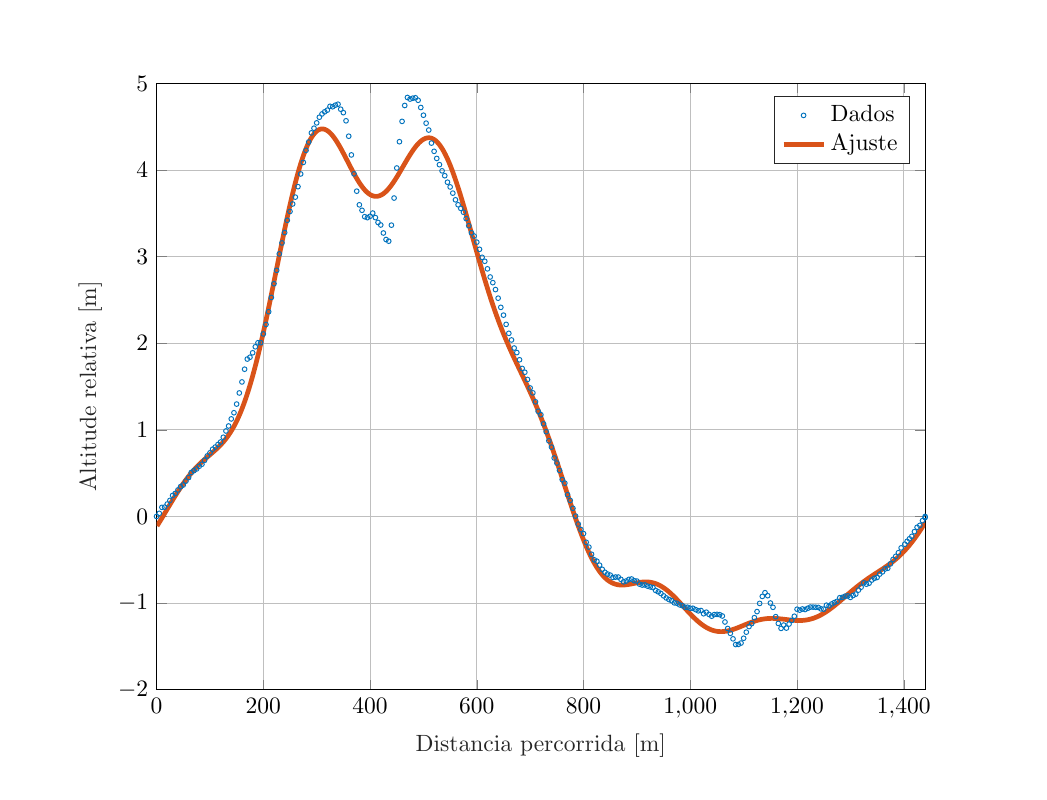
\begin{tikzpicture}[scale=0.85]

\begin{axis}[%
width=4.521in,
height=3.566in,
at={(0.758in,0.481in)},
scale only axis,
xmin=0,
xmax=1440,
xlabel style={font=\color{white!15!black}},
xlabel={Distancia percorrida [m]},
ymin=-2,
ymax=5,
ylabel style={font=\color{white!15!black}},
ylabel={Altitude relativa [m]},
axis background/.style={fill=white},
xmajorgrids,
ymajorgrids,
legend style={legend cell align=left, align=left, draw=white!15!black}
]
\addplot [color=mycolor1, only marks, mark size=1.0pt, mark=o, mark options={solid, mycolor1}]
  table[row sep=crcr]{%
0	0\\
5.1222	0.035738\\
10.052	0.10497\\
15.102	0.10772\\
20.056	0.14341\\
25.018	0.18539\\
30.099	0.24281\\
35.019	0.26534\\
40.103	0.30621\\
45.03	0.34432\\
50.02	0.36324\\
55.06	0.4084\\
60.082	0.44874\\
65.003	0.50745\\
70.013	0.52866\\
75.043	0.54874\\
80.029	0.58008\\
85.054	0.60309\\
90.004	0.64756\\
95.034	0.69913\\
100.08	0.73437\\
105.09	0.77665\\
110.03	0.80147\\
115.11	0.8308\\
120.05	0.85947\\
125.08	0.91471\\
130.04	0.987\\
135.06	1.0446\\
140.02	1.1265\\
145.07	1.1976\\
150.07	1.2977\\
155.07	1.4261\\
160.05	1.5534\\
165.02	1.7003\\
170.06	1.8176\\
175.03	1.8384\\
180.1	1.8899\\
185.09	1.959\\
190.08	2.0057\\
195.07	2.0065\\
200.08	2.1076\\
205.05	2.2171\\
210.04	2.3643\\
215.1	2.5291\\
220.07	2.6873\\
225.1	2.8419\\
230.05	3.0317\\
235.08	3.1583\\
240.02	3.2784\\
245.01	3.4202\\
250.02	3.5219\\
255.05	3.6083\\
260.01	3.6875\\
265	3.8082\\
270.07	3.9549\\
275.02	4.0884\\
280.08	4.2276\\
285.07	4.3234\\
290.09	4.4291\\
295.02	4.4829\\
300.06	4.5449\\
305.07	4.61\\
310.07	4.648\\
315.05	4.6728\\
320.01	4.6917\\
325.05	4.7362\\
330.01	4.7312\\
335.08	4.7492\\
340.01	4.7603\\
345.05	4.7026\\
350.06	4.6628\\
355.04	4.5688\\
360.09	4.3908\\
365.05	4.1747\\
370.01	3.9563\\
375.05	3.7561\\
380.01	3.5984\\
385.01	3.5353\\
390.02	3.4615\\
395.07	3.4505\\
400.1	3.4657\\
405.04	3.5032\\
410.05	3.4511\\
415	3.3952\\
420.07	3.3656\\
425.01	3.2732\\
430.02	3.1978\\
435.03	3.1787\\
440.06	3.3637\\
445.07	3.6768\\
450.11	4.0237\\
455.11	4.3273\\
460.03	4.5621\\
465.01	4.7456\\
470.09	4.8381\\
475.01	4.8199\\
480.09	4.8295\\
485	4.8346\\
490.09	4.8057\\
495.09	4.7223\\
500.09	4.6332\\
505.1	4.5413\\
510.02	4.4621\\
515.05	4.3114\\
520.05	4.2162\\
525.01	4.134\\
530.04	4.0624\\
535.01	3.9909\\
540	3.9346\\
545.08	3.8595\\
550.12	3.8051\\
555.1	3.7335\\
560.09	3.6563\\
565.02	3.599\\
570.06	3.5572\\
575.09	3.5131\\
580.08	3.4391\\
585	3.3567\\
590.01	3.2757\\
595.05	3.2379\\
600.02	3.1674\\
605.08	3.0848\\
610.02	2.9922\\
615	2.9465\\
620.02	2.8593\\
625.11	2.7651\\
630.08	2.6997\\
635.08	2.6199\\
640.02	2.5204\\
645.04	2.4145\\
650.07	2.3246\\
655	2.2181\\
660.06	2.1146\\
665.02	2.038\\
670.06	1.9449\\
675.05	1.8925\\
680.09	1.8092\\
685.08	1.709\\
690.04	1.6652\\
695.04	1.5816\\
700.02	1.4836\\
705.1	1.4271\\
710.02	1.3237\\
715	1.2147\\
720.11	1.1747\\
725.08	1.0693\\
730.02	0.9783\\
735.02	0.87326\\
740.01	0.80079\\
745.06	0.67547\\
750.09	0.61633\\
755.06	0.53173\\
760.08	0.42591\\
765	0.38467\\
770.1	0.25097\\
775.04	0.185\\
780.1	0.094467\\
785.11	0.0042468\\
790.01	-0.087749\\
795.03	-0.15127\\
800.04	-0.19791\\
805.06	-0.29861\\
810.07	-0.35415\\
815.01	-0.43642\\
820.07	-0.50071\\
825.05	-0.5167\\
830.08	-0.56259\\
835.08	-0.6105\\
840.01	-0.64431\\
845.08	-0.66497\\
850.11	-0.67766\\
855.07	-0.70386\\
860.02	-0.69959\\
865.1	-0.70008\\
870.02	-0.72612\\
875.09	-0.75503\\
880.11	-0.74512\\
885.04	-0.72702\\
890.06	-0.72219\\
895.01	-0.74177\\
900.04	-0.74645\\
905.09	-0.78183\\
910.06	-0.79228\\
915.01	-0.79059\\
920.11	-0.80498\\
925	-0.81388\\
930.09	-0.82108\\
935.08	-0.85434\\
940.08	-0.87037\\
945.02	-0.8898\\
950.11	-0.91711\\
955	-0.941\\
960.02	-0.95908\\
965.01	-0.97259\\
970.07	-0.9977\\
975.02	-1.0021\\
980.02	-1.0205\\
985.06	-1.03\\
990.07	-1.0475\\
995.09	-1.0488\\
1000.1	-1.0607\\
1005	-1.0603\\
1010.1	-1.0762\\
1015	-1.0899\\
1020.1	-1.0865\\
1025	-1.1233\\
1030	-1.1057\\
1035.1	-1.1309\\
1040.1	-1.1516\\
1045.1	-1.1333\\
1050.1	-1.1306\\
1055	-1.1343\\
1060.1	-1.1496\\
1065	-1.2185\\
1070.1	-1.294\\
1075.1	-1.3496\\
1080.1	-1.4133\\
1085.1	-1.4789\\
1090.1	-1.4778\\
1095.1	-1.4619\\
1100	-1.4065\\
1105	-1.3362\\
1110.1	-1.2712\\
1115.1	-1.2374\\
1120.1	-1.1685\\
1125.1	-1.0986\\
1130	-1.0041\\
1135	-0.92332\\
1140	-0.88023\\
1145.1	-0.91493\\
1150.1	-0.9995\\
1155	-1.0491\\
1160.1	-1.1572\\
1165	-1.2352\\
1170.1	-1.2925\\
1175	-1.2543\\
1180.1	-1.2889\\
1185.1	-1.2424\\
1190.1	-1.2007\\
1195	-1.1524\\
1200.1	-1.0711\\
1205	-1.0818\\
1210	-1.0683\\
1215.1	-1.0743\\
1220	-1.0607\\
1225	-1.0466\\
1230.1	-1.0469\\
1235.1	-1.049\\
1240	-1.0506\\
1245	-1.0674\\
1250	-1.0704\\
1255.1	-1.0248\\
1260.1	-1.0326\\
1265	-1.0105\\
1270.1	-0.99422\\
1275	-0.98019\\
1280.1	-0.93839\\
1285	-0.93409\\
1290.1	-0.92035\\
1295.1	-0.9174\\
1300	-0.93492\\
1305.1	-0.91239\\
1310.1	-0.89661\\
1315.1	-0.85047\\
1320.1	-0.81659\\
1325.1	-0.76624\\
1330.1	-0.78241\\
1335	-0.77116\\
1340.1	-0.73442\\
1345.1	-0.71422\\
1350	-0.70423\\
1355	-0.66556\\
1360.1	-0.63987\\
1365.1	-0.60605\\
1370	-0.59789\\
1375	-0.54782\\
1380	-0.49583\\
1385	-0.46034\\
1390	-0.41838\\
1395.1	-0.363\\
1401.9	-0.32049\\
1406.3	-0.28726\\
1410.6	-0.25818\\
1415.1	-0.22964\\
1420	-0.17512\\
1425	-0.12472\\
1430.1	-0.10287\\
1435.1	-0.048184\\
1440	-0.01308\\
1440	0\\
1445.1222	0.035738\\
1450.052	0.10497\\
1455.102	0.10772\\
1460.056	0.14341\\
1465.018	0.18539\\
1470.099	0.24281\\
1475.019	0.26534\\
1480.103	0.30621\\
1485.03	0.34432\\
1490.02	0.36324\\
1495.06	0.4084\\
1500.082	0.44874\\
1505.003	0.50745\\
1510.013	0.52866\\
1515.043	0.54874\\
1520.029	0.58008\\
1525.054	0.60309\\
1530.004	0.64756\\
1535.034	0.69913\\
1540.08	0.73437\\
1545.09	0.77665\\
1550.03	0.80147\\
1555.11	0.8308\\
1560.05	0.85947\\
1565.08	0.91471\\
1570.04	0.987\\
1575.06	1.0446\\
1580.02	1.1265\\
1585.07	1.1976\\
1590.07	1.2977\\
1595.07	1.4261\\
1600.05	1.5534\\
1605.02	1.7003\\
1610.06	1.8176\\
1615.03	1.8384\\
1620.1	1.8899\\
1625.09	1.959\\
1630.08	2.0057\\
1635.07	2.0065\\
1640.08	2.1076\\
1645.05	2.2171\\
1650.04	2.3643\\
1655.1	2.5291\\
1660.07	2.6873\\
1665.1	2.8419\\
1670.05	3.0317\\
1675.08	3.1583\\
1680.02	3.2784\\
1685.01	3.4202\\
1690.02	3.5219\\
1695.05	3.6083\\
1700.01	3.6875\\
1705	3.8082\\
1710.07	3.9549\\
1715.02	4.0884\\
1720.08	4.2276\\
1725.07	4.3234\\
1730.09	4.4291\\
1735.02	4.4829\\
1740.06	4.5449\\
1745.07	4.61\\
1750.07	4.648\\
1755.05	4.6728\\
1760.01	4.6917\\
1765.05	4.7362\\
1770.01	4.7312\\
1775.08	4.7492\\
1780.01	4.7603\\
1785.05	4.7026\\
1790.06	4.6628\\
1795.04	4.5688\\
1800.09	4.3908\\
1805.05	4.1747\\
1810.01	3.9563\\
1815.05	3.7561\\
1820.01	3.5984\\
1825.01	3.5353\\
1830.02	3.4615\\
1835.07	3.4505\\
1840.1	3.4657\\
1845.04	3.5032\\
1850.05	3.4511\\
1855	3.3952\\
1860.07	3.3656\\
1865.01	3.2732\\
1870.02	3.1978\\
1875.03	3.1787\\
1880.06	3.3637\\
1885.07	3.6768\\
1890.11	4.0237\\
1895.11	4.3273\\
1900.03	4.5621\\
1905.01	4.7456\\
1910.09	4.8381\\
1915.01	4.8199\\
1920.09	4.8295\\
1925	4.8346\\
1930.09	4.8057\\
1935.09	4.7223\\
1940.09	4.6332\\
1945.1	4.5413\\
1950.02	4.4621\\
1955.05	4.3114\\
1960.05	4.2162\\
1965.01	4.134\\
1970.04	4.0624\\
1975.01	3.9909\\
1980	3.9346\\
1985.08	3.8595\\
1990.12	3.8051\\
1995.1	3.7335\\
2000.09	3.6563\\
2005.02	3.599\\
2010.06	3.5572\\
2015.09	3.5131\\
2020.08	3.4391\\
2025	3.3567\\
2030.01	3.2757\\
2035.05	3.2379\\
2040.02	3.1674\\
2045.08	3.0848\\
2050.02	2.9922\\
2055	2.9465\\
2060.02	2.8593\\
2065.11	2.7651\\
2070.08	2.6997\\
2075.08	2.6199\\
2080.02	2.5204\\
2085.04	2.4145\\
2090.07	2.3246\\
2095	2.2181\\
2100.06	2.1146\\
2105.02	2.038\\
2110.06	1.9449\\
2115.05	1.8925\\
2120.09	1.8092\\
2125.08	1.709\\
2130.04	1.6652\\
2135.04	1.5816\\
2140.02	1.4836\\
2145.1	1.4271\\
2150.02	1.3237\\
2155	1.2147\\
2160.11	1.1747\\
2165.08	1.0693\\
2170.02	0.9783\\
2175.02	0.87326\\
2180.01	0.80079\\
2185.06	0.67547\\
2190.09	0.61633\\
2195.06	0.53173\\
2200.08	0.42591\\
2205	0.38467\\
2210.1	0.25097\\
2215.04	0.185\\
2220.1	0.094467\\
2225.11	0.0042468\\
2230.01	-0.087749\\
2235.03	-0.15127\\
2240.04	-0.19791\\
2245.06	-0.29861\\
2250.07	-0.35415\\
2255.01	-0.43642\\
2260.07	-0.50071\\
2265.05	-0.5167\\
2270.08	-0.56259\\
2275.08	-0.6105\\
2280.01	-0.64431\\
2285.08	-0.66497\\
2290.11	-0.67766\\
2295.07	-0.70386\\
2300.02	-0.69959\\
2305.1	-0.70008\\
2310.02	-0.72612\\
2315.09	-0.75503\\
2320.11	-0.74512\\
2325.04	-0.72702\\
2330.06	-0.72219\\
2335.01	-0.74177\\
2340.04	-0.74645\\
2345.09	-0.78183\\
2350.06	-0.79228\\
2355.01	-0.79059\\
2360.11	-0.80498\\
2365	-0.81388\\
2370.09	-0.82108\\
2375.08	-0.85434\\
2380.08	-0.87037\\
2385.02	-0.8898\\
2390.11	-0.91711\\
2395	-0.941\\
2400.02	-0.95908\\
2405.01	-0.97259\\
2410.07	-0.9977\\
2415.02	-1.0021\\
2420.02	-1.0205\\
2425.06	-1.03\\
2430.07	-1.0475\\
2435.09	-1.0488\\
2440.1	-1.0607\\
2445	-1.0603\\
2450.1	-1.0762\\
2455	-1.0899\\
2460.1	-1.0865\\
2465	-1.1233\\
2470	-1.1057\\
2475.1	-1.1309\\
2480.1	-1.1516\\
2485.1	-1.1333\\
2490.1	-1.1306\\
2495	-1.1343\\
2500.1	-1.1496\\
2505	-1.2185\\
2510.1	-1.294\\
2515.1	-1.3496\\
2520.1	-1.4133\\
2525.1	-1.4789\\
2530.1	-1.4778\\
2535.1	-1.4619\\
2540	-1.4065\\
2545	-1.3362\\
2550.1	-1.2712\\
2555.1	-1.2374\\
2560.1	-1.1685\\
2565.1	-1.0986\\
2570	-1.0041\\
2575	-0.92332\\
2580	-0.88023\\
2585.1	-0.91493\\
2590.1	-0.9995\\
2595	-1.0491\\
2600.1	-1.1572\\
2605	-1.2352\\
2610.1	-1.2925\\
2615	-1.2543\\
2620.1	-1.2889\\
2625.1	-1.2424\\
2630.1	-1.2007\\
2635	-1.1524\\
2640.1	-1.0711\\
2645	-1.0818\\
2650	-1.0683\\
2655.1	-1.0743\\
2660	-1.0607\\
2665	-1.0466\\
2670.1	-1.0469\\
2675.1	-1.049\\
2680	-1.0506\\
2685	-1.0674\\
2690	-1.0704\\
2695.1	-1.0248\\
2700.1	-1.0326\\
2705	-1.0105\\
2710.1	-0.99422\\
2715	-0.98019\\
2720.1	-0.93839\\
2725	-0.93409\\
2730.1	-0.92035\\
2735.1	-0.9174\\
2740	-0.93492\\
2745.1	-0.91239\\
2750.1	-0.89661\\
2755.1	-0.85047\\
2760.1	-0.81659\\
2765.1	-0.76624\\
2770.1	-0.78241\\
2775	-0.77116\\
2780.1	-0.73442\\
2785.1	-0.71422\\
2790	-0.70423\\
2795	-0.66556\\
2800.1	-0.63987\\
2805.1	-0.60605\\
2810	-0.59789\\
2815	-0.54782\\
2820	-0.49583\\
2825	-0.46034\\
2830	-0.41838\\
2835.1	-0.363\\
2841.9	-0.32049\\
2846.3	-0.28726\\
2850.6	-0.25818\\
2855.1	-0.22964\\
2860	-0.17512\\
2865	-0.12472\\
2870.1	-0.10287\\
2875.1	-0.048184\\
2880	-0.01308\\
2880	0\\
2885.1222	0.035738\\
2890.052	0.10497\\
2895.102	0.10772\\
2900.056	0.14341\\
2905.018	0.18539\\
2910.099	0.24281\\
2915.019	0.26534\\
2920.103	0.30621\\
2925.03	0.34432\\
2930.02	0.36324\\
2935.06	0.4084\\
2940.082	0.44874\\
2945.003	0.50745\\
2950.013	0.52866\\
2955.043	0.54874\\
2960.029	0.58008\\
2965.054	0.60309\\
2970.004	0.64756\\
2975.034	0.69913\\
2980.08	0.73437\\
2985.09	0.77665\\
2990.03	0.80147\\
2995.11	0.8308\\
3000.05	0.85947\\
3005.08	0.91471\\
3010.04	0.987\\
3015.06	1.0446\\
3020.02	1.1265\\
3025.07	1.1976\\
3030.07	1.2977\\
3035.07	1.4261\\
3040.05	1.5534\\
3045.02	1.7003\\
3050.06	1.8176\\
3055.03	1.8384\\
3060.1	1.8899\\
3065.09	1.959\\
3070.08	2.0057\\
3075.07	2.0065\\
3080.08	2.1076\\
3085.05	2.2171\\
3090.04	2.3643\\
3095.1	2.5291\\
3100.07	2.6873\\
3105.1	2.8419\\
3110.05	3.0317\\
3115.08	3.1583\\
3120.02	3.2784\\
3125.01	3.4202\\
3130.02	3.5219\\
3135.05	3.6083\\
3140.01	3.6875\\
3145	3.8082\\
3150.07	3.9549\\
3155.02	4.0884\\
3160.08	4.2276\\
3165.07	4.3234\\
3170.09	4.4291\\
3175.02	4.4829\\
3180.06	4.5449\\
3185.07	4.61\\
3190.07	4.648\\
3195.05	4.6728\\
3200.01	4.6917\\
3205.05	4.7362\\
3210.01	4.7312\\
3215.08	4.7492\\
3220.01	4.7603\\
3225.05	4.7026\\
3230.06	4.6628\\
3235.04	4.5688\\
3240.09	4.3908\\
3245.05	4.1747\\
3250.01	3.9563\\
3255.05	3.7561\\
3260.01	3.5984\\
3265.01	3.5353\\
3270.02	3.4615\\
3275.07	3.4505\\
3280.1	3.4657\\
3285.04	3.5032\\
3290.05	3.4511\\
3295	3.3952\\
3300.07	3.3656\\
3305.01	3.2732\\
3310.02	3.1978\\
3315.03	3.1787\\
3320.06	3.3637\\
3325.07	3.6768\\
3330.11	4.0237\\
3335.11	4.3273\\
3340.03	4.5621\\
3345.01	4.7456\\
3350.09	4.8381\\
3355.01	4.8199\\
3360.09	4.8295\\
3365	4.8346\\
3370.09	4.8057\\
3375.09	4.7223\\
3380.09	4.6332\\
3385.1	4.5413\\
3390.02	4.4621\\
3395.05	4.3114\\
3400.05	4.2162\\
3405.01	4.134\\
3410.04	4.0624\\
3415.01	3.9909\\
3420	3.9346\\
3425.08	3.8595\\
3430.12	3.8051\\
3435.1	3.7335\\
3440.09	3.6563\\
3445.02	3.599\\
3450.06	3.5572\\
3455.09	3.5131\\
3460.08	3.4391\\
3465	3.3567\\
3470.01	3.2757\\
3475.05	3.2379\\
3480.02	3.1674\\
3485.08	3.0848\\
3490.02	2.9922\\
3495	2.9465\\
3500.02	2.8593\\
3505.11	2.7651\\
3510.08	2.6997\\
3515.08	2.6199\\
3520.02	2.5204\\
3525.04	2.4145\\
3530.07	2.3246\\
3535	2.2181\\
3540.06	2.1146\\
3545.02	2.038\\
3550.06	1.9449\\
3555.05	1.8925\\
3560.09	1.8092\\
3565.08	1.709\\
3570.04	1.6652\\
3575.04	1.5816\\
3580.02	1.4836\\
3585.1	1.4271\\
3590.02	1.3237\\
3595	1.2147\\
3600.11	1.1747\\
3605.08	1.0693\\
3610.02	0.9783\\
3615.02	0.87326\\
3620.01	0.80079\\
3625.06	0.67547\\
3630.09	0.61633\\
3635.06	0.53173\\
3640.08	0.42591\\
3645	0.38467\\
3650.1	0.25097\\
3655.04	0.185\\
3660.1	0.094467\\
3665.11	0.0042468\\
3670.01	-0.087749\\
3675.03	-0.15127\\
3680.04	-0.19791\\
3685.06	-0.29861\\
3690.07	-0.35415\\
3695.01	-0.43642\\
3700.07	-0.50071\\
3705.05	-0.5167\\
3710.08	-0.56259\\
3715.08	-0.6105\\
3720.01	-0.64431\\
3725.08	-0.66497\\
3730.11	-0.67766\\
3735.07	-0.70386\\
3740.02	-0.69959\\
3745.1	-0.70008\\
3750.02	-0.72612\\
3755.09	-0.75503\\
3760.11	-0.74512\\
3765.04	-0.72702\\
3770.06	-0.72219\\
3775.01	-0.74177\\
3780.04	-0.74645\\
3785.09	-0.78183\\
3790.06	-0.79228\\
3795.01	-0.79059\\
3800.11	-0.80498\\
3805	-0.81388\\
3810.09	-0.82108\\
3815.08	-0.85434\\
3820.08	-0.87037\\
3825.02	-0.8898\\
3830.11	-0.91711\\
3835	-0.941\\
3840.02	-0.95908\\
3845.01	-0.97259\\
3850.07	-0.9977\\
3855.02	-1.0021\\
3860.02	-1.0205\\
3865.06	-1.03\\
3870.07	-1.0475\\
3875.09	-1.0488\\
3880.1	-1.0607\\
3885	-1.0603\\
3890.1	-1.0762\\
3895	-1.0899\\
3900.1	-1.0865\\
3905	-1.1233\\
3910	-1.1057\\
3915.1	-1.1309\\
3920.1	-1.1516\\
3925.1	-1.1333\\
3930.1	-1.1306\\
3935	-1.1343\\
3940.1	-1.1496\\
3945	-1.2185\\
3950.1	-1.294\\
3955.1	-1.3496\\
3960.1	-1.4133\\
3965.1	-1.4789\\
3970.1	-1.4778\\
3975.1	-1.4619\\
3980	-1.4065\\
3985	-1.3362\\
3990.1	-1.2712\\
3995.1	-1.2374\\
4000.1	-1.1685\\
4005.1	-1.0986\\
4010	-1.0041\\
4015	-0.92332\\
4020	-0.88023\\
4025.1	-0.91493\\
4030.1	-0.9995\\
4035	-1.0491\\
4040.1	-1.1572\\
4045	-1.2352\\
4050.1	-1.2925\\
4055	-1.2543\\
4060.1	-1.2889\\
4065.1	-1.2424\\
4070.1	-1.2007\\
4075	-1.1524\\
4080.1	-1.0711\\
4085	-1.0818\\
4090	-1.0683\\
4095.1	-1.0743\\
4100	-1.0607\\
4105	-1.0466\\
4110.1	-1.0469\\
4115.1	-1.049\\
4120	-1.0506\\
4125	-1.0674\\
4130	-1.0704\\
4135.1	-1.0248\\
4140.1	-1.0326\\
4145	-1.0105\\
4150.1	-0.99422\\
4155	-0.98019\\
4160.1	-0.93839\\
4165	-0.93409\\
4170.1	-0.92035\\
4175.1	-0.9174\\
4180	-0.93492\\
4185.1	-0.91239\\
4190.1	-0.89661\\
4195.1	-0.85047\\
4200.1	-0.81659\\
4205.1	-0.76624\\
4210.1	-0.78241\\
4215	-0.77116\\
4220.1	-0.73442\\
4225.1	-0.71422\\
4230	-0.70423\\
4235	-0.66556\\
4240.1	-0.63987\\
4245.1	-0.60605\\
4250	-0.59789\\
4255	-0.54782\\
4260	-0.49583\\
4265	-0.46034\\
4270	-0.41838\\
4275.1	-0.363\\
4281.9	-0.32049\\
4286.3	-0.28726\\
4290.6	-0.25818\\
4295.1	-0.22964\\
4300	-0.17512\\
4305	-0.12472\\
4310.1	-0.10287\\
4315.1	-0.048184\\
4320	-0.01308\\
4320	0\\
4325.1222	0.035738\\
4330.052	0.10497\\
4335.102	0.10772\\
4340.056	0.14341\\
4345.018	0.18539\\
4350.099	0.24281\\
4355.019	0.26534\\
4360.103	0.30621\\
4365.03	0.34432\\
4370.02	0.36324\\
4375.06	0.4084\\
4380.082	0.44874\\
4385.003	0.50745\\
4390.013	0.52866\\
4395.043	0.54874\\
4400.029	0.58008\\
4405.054	0.60309\\
4410.004	0.64756\\
4415.034	0.69913\\
4420.08	0.73437\\
4425.09	0.77665\\
4430.03	0.80147\\
4435.11	0.8308\\
4440.05	0.85947\\
4445.08	0.91471\\
4450.04	0.987\\
4455.06	1.0446\\
4460.02	1.1265\\
4465.07	1.1976\\
4470.07	1.2977\\
4475.07	1.4261\\
4480.05	1.5534\\
4485.02	1.7003\\
4490.06	1.8176\\
4495.03	1.8384\\
4500.1	1.8899\\
4505.09	1.959\\
4510.08	2.0057\\
4515.07	2.0065\\
4520.08	2.1076\\
4525.05	2.2171\\
4530.04	2.3643\\
4535.1	2.5291\\
4540.07	2.6873\\
4545.1	2.8419\\
4550.05	3.0317\\
4555.08	3.1583\\
4560.02	3.2784\\
4565.01	3.4202\\
4570.02	3.5219\\
4575.05	3.6083\\
4580.01	3.6875\\
4585	3.8082\\
4590.07	3.9549\\
4595.02	4.0884\\
4600.08	4.2276\\
4605.07	4.3234\\
4610.09	4.4291\\
4615.02	4.4829\\
4620.06	4.5449\\
4625.07	4.61\\
4630.07	4.648\\
4635.05	4.6728\\
4640.01	4.6917\\
4645.05	4.7362\\
4650.01	4.7312\\
4655.08	4.7492\\
4660.01	4.7603\\
4665.05	4.7026\\
4670.06	4.6628\\
4675.04	4.5688\\
4680.09	4.3908\\
4685.05	4.1747\\
4690.01	3.9563\\
4695.05	3.7561\\
4700.01	3.5984\\
4705.01	3.5353\\
4710.02	3.4615\\
4715.07	3.4505\\
4720.1	3.4657\\
4725.04	3.5032\\
4730.05	3.4511\\
4735	3.3952\\
4740.07	3.3656\\
4745.01	3.2732\\
4750.02	3.1978\\
4755.03	3.1787\\
4760.06	3.3637\\
4765.07	3.6768\\
4770.11	4.0237\\
4775.11	4.3273\\
4780.03	4.5621\\
4785.01	4.7456\\
4790.09	4.8381\\
4795.01	4.8199\\
4800.09	4.8295\\
4805	4.8346\\
4810.09	4.8057\\
4815.09	4.7223\\
4820.09	4.6332\\
4825.1	4.5413\\
4830.02	4.4621\\
4835.05	4.3114\\
4840.05	4.2162\\
4845.01	4.134\\
4850.04	4.0624\\
4855.01	3.9909\\
4860	3.9346\\
4865.08	3.8595\\
4870.12	3.8051\\
4875.1	3.7335\\
4880.09	3.6563\\
4885.02	3.599\\
4890.06	3.5572\\
4895.09	3.5131\\
4900.08	3.4391\\
4905	3.3567\\
4910.01	3.2757\\
4915.05	3.2379\\
4920.02	3.1674\\
4925.08	3.0848\\
4930.02	2.9922\\
4935	2.9465\\
4940.02	2.8593\\
4945.11	2.7651\\
4950.08	2.6997\\
4955.08	2.6199\\
4960.02	2.5204\\
4965.04	2.4145\\
4970.07	2.3246\\
4975	2.2181\\
4980.06	2.1146\\
4985.02	2.038\\
4990.06	1.9449\\
4995.05	1.8925\\
5000.09	1.8092\\
5005.08	1.709\\
5010.04	1.6652\\
5015.04	1.5816\\
5020.02	1.4836\\
5025.1	1.4271\\
5030.02	1.3237\\
5035	1.2147\\
5040.11	1.1747\\
5045.08	1.0693\\
5050.02	0.9783\\
5055.02	0.87326\\
5060.01	0.80079\\
5065.06	0.67547\\
5070.09	0.61633\\
5075.06	0.53173\\
5080.08	0.42591\\
5085	0.38467\\
5090.1	0.25097\\
5095.04	0.185\\
5100.1	0.094467\\
5105.11	0.0042468\\
5110.01	-0.087749\\
5115.03	-0.15127\\
5120.04	-0.19791\\
5125.06	-0.29861\\
5130.07	-0.35415\\
5135.01	-0.43642\\
5140.07	-0.50071\\
5145.05	-0.5167\\
5150.08	-0.56259\\
5155.08	-0.6105\\
5160.01	-0.64431\\
5165.08	-0.66497\\
5170.11	-0.67766\\
5175.07	-0.70386\\
5180.02	-0.69959\\
5185.1	-0.70008\\
5190.02	-0.72612\\
5195.09	-0.75503\\
5200.11	-0.74512\\
5205.04	-0.72702\\
5210.06	-0.72219\\
5215.01	-0.74177\\
5220.04	-0.74645\\
5225.09	-0.78183\\
5230.06	-0.79228\\
5235.01	-0.79059\\
5240.11	-0.80498\\
5245	-0.81388\\
5250.09	-0.82108\\
5255.08	-0.85434\\
5260.08	-0.87037\\
5265.02	-0.8898\\
5270.11	-0.91711\\
5275	-0.941\\
5280.02	-0.95908\\
5285.01	-0.97259\\
5290.07	-0.9977\\
5295.02	-1.0021\\
5300.02	-1.0205\\
5305.06	-1.03\\
5310.07	-1.0475\\
5315.09	-1.0488\\
5320.1	-1.0607\\
5325	-1.0603\\
5330.1	-1.0762\\
5335	-1.0899\\
5340.1	-1.0865\\
5345	-1.1233\\
5350	-1.1057\\
5355.1	-1.1309\\
5360.1	-1.1516\\
5365.1	-1.1333\\
5370.1	-1.1306\\
5375	-1.1343\\
5380.1	-1.1496\\
5385	-1.2185\\
5390.1	-1.294\\
5395.1	-1.3496\\
5400.1	-1.4133\\
5405.1	-1.4789\\
5410.1	-1.4778\\
5415.1	-1.4619\\
5420	-1.4065\\
5425	-1.3362\\
5430.1	-1.2712\\
5435.1	-1.2374\\
5440.1	-1.1685\\
5445.1	-1.0986\\
5450	-1.0041\\
5455	-0.92332\\
5460	-0.88023\\
5465.1	-0.91493\\
5470.1	-0.9995\\
5475	-1.0491\\
5480.1	-1.1572\\
5485	-1.2352\\
5490.1	-1.2925\\
5495	-1.2543\\
5500.1	-1.2889\\
5505.1	-1.2424\\
5510.1	-1.2007\\
5515	-1.1524\\
5520.1	-1.0711\\
5525	-1.0818\\
5530	-1.0683\\
5535.1	-1.0743\\
5540	-1.0607\\
5545	-1.0466\\
5550.1	-1.0469\\
5555.1	-1.049\\
5560	-1.0506\\
5565	-1.0674\\
5570	-1.0704\\
5575.1	-1.0248\\
5580.1	-1.0326\\
5585	-1.0105\\
5590.1	-0.99422\\
5595	-0.98019\\
5600.1	-0.93839\\
5605	-0.93409\\
5610.1	-0.92035\\
5615.1	-0.9174\\
5620	-0.93492\\
5625.1	-0.91239\\
5630.1	-0.89661\\
5635.1	-0.85047\\
5640.1	-0.81659\\
5645.1	-0.76624\\
5650.1	-0.78241\\
5655	-0.77116\\
5660.1	-0.73442\\
5665.1	-0.71422\\
5670	-0.70423\\
5675	-0.66556\\
5680.1	-0.63987\\
5685.1	-0.60605\\
5690	-0.59789\\
5695	-0.54782\\
5700	-0.49583\\
5705	-0.46034\\
5710	-0.41838\\
5715.1	-0.363\\
5721.9	-0.32049\\
5726.3	-0.28726\\
5730.6	-0.25818\\
5735.1	-0.22964\\
5740	-0.17512\\
5745	-0.12472\\
5750.1	-0.10287\\
5755.1	-0.048184\\
5760	-0.01308\\
5760	0\\
5765.1222	0.035738\\
5770.052	0.10497\\
5775.102	0.10772\\
5780.056	0.14341\\
5785.018	0.18539\\
5790.099	0.24281\\
5795.019	0.26534\\
5800.103	0.30621\\
5805.03	0.34432\\
5810.02	0.36324\\
5815.06	0.4084\\
5820.082	0.44874\\
5825.003	0.50745\\
5830.013	0.52866\\
5835.043	0.54874\\
5840.029	0.58008\\
5845.054	0.60309\\
5850.004	0.64756\\
5855.034	0.69913\\
5860.08	0.73437\\
5865.09	0.77665\\
5870.03	0.80147\\
5875.11	0.8308\\
5880.05	0.85947\\
5885.08	0.91471\\
5890.04	0.987\\
5895.06	1.0446\\
5900.02	1.1265\\
5905.07	1.1976\\
5910.07	1.2977\\
5915.07	1.4261\\
5920.05	1.5534\\
5925.02	1.7003\\
5930.06	1.8176\\
5935.03	1.8384\\
5940.1	1.8899\\
5945.09	1.959\\
5950.08	2.0057\\
5955.07	2.0065\\
5960.08	2.1076\\
5965.05	2.2171\\
5970.04	2.3643\\
5975.1	2.5291\\
5980.07	2.6873\\
5985.1	2.8419\\
5990.05	3.0317\\
5995.08	3.1583\\
6000.02	3.2784\\
6005.01	3.4202\\
6010.02	3.5219\\
6015.05	3.6083\\
6020.01	3.6875\\
6025	3.8082\\
6030.07	3.9549\\
6035.02	4.0884\\
6040.08	4.2276\\
6045.07	4.3234\\
6050.09	4.4291\\
6055.02	4.4829\\
6060.06	4.5449\\
6065.07	4.61\\
6070.07	4.648\\
6075.05	4.6728\\
6080.01	4.6917\\
6085.05	4.7362\\
6090.01	4.7312\\
6095.08	4.7492\\
6100.01	4.7603\\
6105.05	4.7026\\
6110.06	4.6628\\
6115.04	4.5688\\
6120.09	4.3908\\
6125.05	4.1747\\
6130.01	3.9563\\
6135.05	3.7561\\
6140.01	3.5984\\
6145.01	3.5353\\
6150.02	3.4615\\
6155.07	3.4505\\
6160.1	3.4657\\
6165.04	3.5032\\
6170.05	3.4511\\
6175	3.3952\\
6180.07	3.3656\\
6185.01	3.2732\\
6190.02	3.1978\\
6195.03	3.1787\\
6200.06	3.3637\\
6205.07	3.6768\\
6210.11	4.0237\\
6215.11	4.3273\\
6220.03	4.5621\\
6225.01	4.7456\\
6230.09	4.8381\\
6235.01	4.8199\\
6240.09	4.8295\\
6245	4.8346\\
6250.09	4.8057\\
6255.09	4.7223\\
6260.09	4.6332\\
6265.1	4.5413\\
6270.02	4.4621\\
6275.05	4.3114\\
6280.05	4.2162\\
6285.01	4.134\\
6290.04	4.0624\\
6295.01	3.9909\\
6300	3.9346\\
6305.08	3.8595\\
6310.12	3.8051\\
6315.1	3.7335\\
6320.09	3.6563\\
6325.02	3.599\\
6330.06	3.5572\\
6335.09	3.5131\\
6340.08	3.4391\\
6345	3.3567\\
6350.01	3.2757\\
6355.05	3.2379\\
6360.02	3.1674\\
6365.08	3.0848\\
6370.02	2.9922\\
6375	2.9465\\
6380.02	2.8593\\
6385.11	2.7651\\
6390.08	2.6997\\
6395.08	2.6199\\
6400.02	2.5204\\
6405.04	2.4145\\
6410.07	2.3246\\
6415	2.2181\\
6420.06	2.1146\\
6425.02	2.038\\
6430.06	1.9449\\
6435.05	1.8925\\
6440.09	1.8092\\
6445.08	1.709\\
6450.04	1.6652\\
6455.04	1.5816\\
6460.02	1.4836\\
6465.1	1.4271\\
6470.02	1.3237\\
6475	1.2147\\
6480.11	1.1747\\
6485.08	1.0693\\
6490.02	0.9783\\
6495.02	0.87326\\
6500.01	0.80079\\
6505.06	0.67547\\
6510.09	0.61633\\
6515.06	0.53173\\
6520.08	0.42591\\
6525	0.38467\\
6530.1	0.25097\\
6535.04	0.185\\
6540.1	0.094467\\
6545.11	0.0042468\\
6550.01	-0.087749\\
6555.03	-0.15127\\
6560.04	-0.19791\\
6565.06	-0.29861\\
6570.07	-0.35415\\
6575.01	-0.43642\\
6580.07	-0.50071\\
6585.05	-0.5167\\
6590.08	-0.56259\\
6595.08	-0.6105\\
6600.01	-0.64431\\
6605.08	-0.66497\\
6610.11	-0.67766\\
6615.07	-0.70386\\
6620.02	-0.69959\\
6625.1	-0.70008\\
6630.02	-0.72612\\
6635.09	-0.75503\\
6640.11	-0.74512\\
6645.04	-0.72702\\
6650.06	-0.72219\\
6655.01	-0.74177\\
6660.04	-0.74645\\
6665.09	-0.78183\\
6670.06	-0.79228\\
6675.01	-0.79059\\
6680.11	-0.80498\\
6685	-0.81388\\
6690.09	-0.82108\\
6695.08	-0.85434\\
6700.08	-0.87037\\
6705.02	-0.8898\\
6710.11	-0.91711\\
6715	-0.941\\
6720.02	-0.95908\\
6725.01	-0.97259\\
6730.07	-0.9977\\
6735.02	-1.0021\\
6740.02	-1.0205\\
6745.06	-1.03\\
6750.07	-1.0475\\
6755.09	-1.0488\\
6760.1	-1.0607\\
6765	-1.0603\\
6770.1	-1.0762\\
6775	-1.0899\\
6780.1	-1.0865\\
6785	-1.1233\\
6790	-1.1057\\
6795.1	-1.1309\\
6800.1	-1.1516\\
6805.1	-1.1333\\
6810.1	-1.1306\\
6815	-1.1343\\
6820.1	-1.1496\\
6825	-1.2185\\
6830.1	-1.294\\
6835.1	-1.3496\\
6840.1	-1.4133\\
6845.1	-1.4789\\
6850.1	-1.4778\\
6855.1	-1.4619\\
6860	-1.4065\\
6865	-1.3362\\
6870.1	-1.2712\\
6875.1	-1.2374\\
6880.1	-1.1685\\
6885.1	-1.0986\\
6890	-1.0041\\
6895	-0.92332\\
6900	-0.88023\\
6905.1	-0.91493\\
6910.1	-0.9995\\
6915	-1.0491\\
6920.1	-1.1572\\
6925	-1.2352\\
6930.1	-1.2925\\
6935	-1.2543\\
6940.1	-1.2889\\
6945.1	-1.2424\\
6950.1	-1.2007\\
6955	-1.1524\\
6960.1	-1.0711\\
6965	-1.0818\\
6970	-1.0683\\
6975.1	-1.0743\\
6980	-1.0607\\
6985	-1.0466\\
6990.1	-1.0469\\
6995.1	-1.049\\
7000	-1.0506\\
7005	-1.0674\\
7010	-1.0704\\
7015.1	-1.0248\\
7020.1	-1.0326\\
7025	-1.0105\\
7030.1	-0.99422\\
7035	-0.98019\\
7040.1	-0.93839\\
7045	-0.93409\\
7050.1	-0.92035\\
7055.1	-0.9174\\
7060	-0.93492\\
7065.1	-0.91239\\
7070.1	-0.89661\\
7075.1	-0.85047\\
7080.1	-0.81659\\
7085.1	-0.76624\\
7090.1	-0.78241\\
7095	-0.77116\\
7100.1	-0.73442\\
7105.1	-0.71422\\
7110	-0.70423\\
7115	-0.66556\\
7120.1	-0.63987\\
7125.1	-0.60605\\
7130	-0.59789\\
7135	-0.54782\\
7140	-0.49583\\
7145	-0.46034\\
7150	-0.41838\\
7155.1	-0.363\\
7161.9	-0.32049\\
7166.3	-0.28726\\
7170.6	-0.25818\\
7175.1	-0.22964\\
7180	-0.17512\\
7185	-0.12472\\
7190.1	-0.10287\\
7195.1	-0.048184\\
7200	-0.01308\\
7200	0\\
7205.1222	0.035738\\
7210.052	0.10497\\
7215.102	0.10772\\
7220.056	0.14341\\
7225.018	0.18539\\
7230.099	0.24281\\
7235.019	0.26534\\
7240.103	0.30621\\
7245.03	0.34432\\
7250.02	0.36324\\
7255.06	0.4084\\
7260.082	0.44874\\
7265.003	0.50745\\
7270.013	0.52866\\
7275.043	0.54874\\
7280.029	0.58008\\
7285.054	0.60309\\
7290.004	0.64756\\
7295.034	0.69913\\
7300.08	0.73437\\
7305.09	0.77665\\
7310.03	0.80147\\
7315.11	0.8308\\
7320.05	0.85947\\
7325.08	0.91471\\
7330.04	0.987\\
7335.06	1.0446\\
7340.02	1.1265\\
7345.07	1.1976\\
7350.07	1.2977\\
7355.07	1.4261\\
7360.05	1.5534\\
7365.02	1.7003\\
7370.06	1.8176\\
7375.03	1.8384\\
7380.1	1.8899\\
7385.09	1.959\\
7390.08	2.0057\\
7395.07	2.0065\\
7400.08	2.1076\\
7405.05	2.2171\\
7410.04	2.3643\\
7415.1	2.5291\\
7420.07	2.6873\\
7425.1	2.8419\\
7430.05	3.0317\\
7435.08	3.1583\\
7440.02	3.2784\\
7445.01	3.4202\\
7450.02	3.5219\\
7455.05	3.6083\\
7460.01	3.6875\\
7465	3.8082\\
7470.07	3.9549\\
7475.02	4.0884\\
7480.08	4.2276\\
7485.07	4.3234\\
7490.09	4.4291\\
7495.02	4.4829\\
7500.06	4.5449\\
7505.07	4.61\\
7510.07	4.648\\
7515.05	4.6728\\
7520.01	4.6917\\
7525.05	4.7362\\
7530.01	4.7312\\
7535.08	4.7492\\
7540.01	4.7603\\
7545.05	4.7026\\
7550.06	4.6628\\
7555.04	4.5688\\
7560.09	4.3908\\
7565.05	4.1747\\
7570.01	3.9563\\
7575.05	3.7561\\
7580.01	3.5984\\
7585.01	3.5353\\
7590.02	3.4615\\
7595.07	3.4505\\
7600.1	3.4657\\
7605.04	3.5032\\
7610.05	3.4511\\
7615	3.3952\\
7620.07	3.3656\\
7625.01	3.2732\\
7630.02	3.1978\\
7635.03	3.1787\\
7640.06	3.3637\\
7645.07	3.6768\\
7650.11	4.0237\\
7655.11	4.3273\\
7660.03	4.5621\\
7665.01	4.7456\\
7670.09	4.8381\\
7675.01	4.8199\\
7680.09	4.8295\\
7685	4.8346\\
7690.09	4.8057\\
7695.09	4.7223\\
7700.09	4.6332\\
7705.1	4.5413\\
7710.02	4.4621\\
7715.05	4.3114\\
7720.05	4.2162\\
7725.01	4.134\\
7730.04	4.0624\\
7735.01	3.9909\\
7740	3.9346\\
7745.08	3.8595\\
7750.12	3.8051\\
7755.1	3.7335\\
7760.09	3.6563\\
7765.02	3.599\\
7770.06	3.5572\\
7775.09	3.5131\\
7780.08	3.4391\\
7785	3.3567\\
7790.01	3.2757\\
7795.05	3.2379\\
7800.02	3.1674\\
7805.08	3.0848\\
7810.02	2.9922\\
7815	2.9465\\
7820.02	2.8593\\
7825.11	2.7651\\
7830.08	2.6997\\
7835.08	2.6199\\
7840.02	2.5204\\
7845.04	2.4145\\
7850.07	2.3246\\
7855	2.2181\\
7860.06	2.1146\\
7865.02	2.038\\
7870.06	1.9449\\
7875.05	1.8925\\
7880.09	1.8092\\
7885.08	1.709\\
7890.04	1.6652\\
7895.04	1.5816\\
7900.02	1.4836\\
7905.1	1.4271\\
7910.02	1.3237\\
7915	1.2147\\
7920.11	1.1747\\
7925.08	1.0693\\
7930.02	0.9783\\
7935.02	0.87326\\
7940.01	0.80079\\
7945.06	0.67547\\
7950.09	0.61633\\
7955.06	0.53173\\
7960.08	0.42591\\
7965	0.38467\\
7970.1	0.25097\\
7975.04	0.185\\
7980.1	0.094467\\
7985.11	0.0042468\\
7990.01	-0.087749\\
7995.03	-0.15127\\
8000.04	-0.19791\\
8005.06	-0.29861\\
8010.07	-0.35415\\
8015.01	-0.43642\\
8020.07	-0.50071\\
8025.05	-0.5167\\
8030.08	-0.56259\\
8035.08	-0.6105\\
8040.01	-0.64431\\
8045.08	-0.66497\\
8050.11	-0.67766\\
8055.07	-0.70386\\
8060.02	-0.69959\\
8065.1	-0.70008\\
8070.02	-0.72612\\
8075.09	-0.75503\\
8080.11	-0.74512\\
8085.04	-0.72702\\
8090.06	-0.72219\\
8095.01	-0.74177\\
8100.04	-0.74645\\
8105.09	-0.78183\\
8110.06	-0.79228\\
8115.01	-0.79059\\
8120.11	-0.80498\\
8125	-0.81388\\
8130.09	-0.82108\\
8135.08	-0.85434\\
8140.08	-0.87037\\
8145.02	-0.8898\\
8150.11	-0.91711\\
8155	-0.941\\
8160.02	-0.95908\\
8165.01	-0.97259\\
8170.07	-0.9977\\
8175.02	-1.0021\\
8180.02	-1.0205\\
8185.06	-1.03\\
8190.07	-1.0475\\
8195.09	-1.0488\\
8200.1	-1.0607\\
8205	-1.0603\\
8210.1	-1.0762\\
8215	-1.0899\\
8220.1	-1.0865\\
8225	-1.1233\\
8230	-1.1057\\
8235.1	-1.1309\\
8240.1	-1.1516\\
8245.1	-1.1333\\
8250.1	-1.1306\\
8255	-1.1343\\
8260.1	-1.1496\\
8265	-1.2185\\
8270.1	-1.294\\
8275.1	-1.3496\\
8280.1	-1.4133\\
8285.1	-1.4789\\
8290.1	-1.4778\\
8295.1	-1.4619\\
8300	-1.4065\\
8305	-1.3362\\
8310.1	-1.2712\\
8315.1	-1.2374\\
8320.1	-1.1685\\
8325.1	-1.0986\\
8330	-1.0041\\
8335	-0.92332\\
8340	-0.88023\\
8345.1	-0.91493\\
8350.1	-0.9995\\
8355	-1.0491\\
8360.1	-1.1572\\
8365	-1.2352\\
8370.1	-1.2925\\
8375	-1.2543\\
8380.1	-1.2889\\
8385.1	-1.2424\\
8390.1	-1.2007\\
8395	-1.1524\\
8400.1	-1.0711\\
8405	-1.0818\\
8410	-1.0683\\
8415.1	-1.0743\\
8420	-1.0607\\
8425	-1.0466\\
8430.1	-1.0469\\
8435.1	-1.049\\
8440	-1.0506\\
8445	-1.0674\\
8450	-1.0704\\
8455.1	-1.0248\\
8460.1	-1.0326\\
8465	-1.0105\\
8470.1	-0.99422\\
8475	-0.98019\\
8480.1	-0.93839\\
8485	-0.93409\\
8490.1	-0.92035\\
8495.1	-0.9174\\
8500	-0.93492\\
8505.1	-0.91239\\
8510.1	-0.89661\\
8515.1	-0.85047\\
8520.1	-0.81659\\
8525.1	-0.76624\\
8530.1	-0.78241\\
8535	-0.77116\\
8540.1	-0.73442\\
8545.1	-0.71422\\
8550	-0.70423\\
8555	-0.66556\\
8560.1	-0.63987\\
8565.1	-0.60605\\
8570	-0.59789\\
8575	-0.54782\\
8580	-0.49583\\
8585	-0.46034\\
8590	-0.41838\\
8595.1	-0.363\\
8601.9	-0.32049\\
8606.3	-0.28726\\
8610.6	-0.25818\\
8615.1	-0.22964\\
8620	-0.17512\\
8625	-0.12472\\
8630.1	-0.10287\\
8635.1	-0.048184\\
8640	-0.01308\\
8640	0\\
8645.1222	0.035738\\
8650.052	0.10497\\
8655.102	0.10772\\
8660.056	0.14341\\
8665.018	0.18539\\
8670.099	0.24281\\
8675.019	0.26534\\
8680.103	0.30621\\
8685.03	0.34432\\
8690.02	0.36324\\
8695.06	0.4084\\
8700.082	0.44874\\
8705.003	0.50745\\
8710.013	0.52866\\
8715.043	0.54874\\
8720.029	0.58008\\
8725.054	0.60309\\
8730.004	0.64756\\
8735.034	0.69913\\
8740.08	0.73437\\
8745.09	0.77665\\
8750.03	0.80147\\
8755.11	0.8308\\
8760.05	0.85947\\
8765.08	0.91471\\
8770.04	0.987\\
8775.06	1.0446\\
8780.02	1.1265\\
8785.07	1.1976\\
8790.07	1.2977\\
8795.07	1.4261\\
8800.05	1.5534\\
8805.02	1.7003\\
8810.06	1.8176\\
8815.03	1.8384\\
8820.1	1.8899\\
8825.09	1.959\\
8830.08	2.0057\\
8835.07	2.0065\\
8840.08	2.1076\\
8845.05	2.2171\\
8850.04	2.3643\\
8855.1	2.5291\\
8860.07	2.6873\\
8865.1	2.8419\\
8870.05	3.0317\\
8875.08	3.1583\\
8880.02	3.2784\\
8885.01	3.4202\\
8890.02	3.5219\\
8895.05	3.6083\\
8900.01	3.6875\\
8905	3.8082\\
8910.07	3.9549\\
8915.02	4.0884\\
8920.08	4.2276\\
8925.07	4.3234\\
8930.09	4.4291\\
8935.02	4.4829\\
8940.06	4.5449\\
8945.07	4.61\\
8950.07	4.648\\
8955.05	4.6728\\
8960.01	4.6917\\
8965.05	4.7362\\
8970.01	4.7312\\
8975.08	4.7492\\
8980.01	4.7603\\
8985.05	4.7026\\
8990.06	4.6628\\
8995.04	4.5688\\
9000.09	4.3908\\
9005.05	4.1747\\
9010.01	3.9563\\
9015.05	3.7561\\
9020.01	3.5984\\
9025.01	3.5353\\
9030.02	3.4615\\
9035.07	3.4505\\
9040.1	3.4657\\
9045.04	3.5032\\
9050.05	3.4511\\
9055	3.3952\\
9060.07	3.3656\\
9065.01	3.2732\\
9070.02	3.1978\\
9075.03	3.1787\\
9080.06	3.3637\\
9085.07	3.6768\\
9090.11	4.0237\\
9095.11	4.3273\\
9100.03	4.5621\\
9105.01	4.7456\\
9110.09	4.8381\\
9115.01	4.8199\\
9120.09	4.8295\\
9125	4.8346\\
9130.09	4.8057\\
9135.09	4.7223\\
9140.09	4.6332\\
9145.1	4.5413\\
9150.02	4.4621\\
9155.05	4.3114\\
9160.05	4.2162\\
9165.01	4.134\\
9170.04	4.0624\\
9175.01	3.9909\\
9180	3.9346\\
9185.08	3.8595\\
9190.12	3.8051\\
9195.1	3.7335\\
9200.09	3.6563\\
9205.02	3.599\\
9210.06	3.5572\\
9215.09	3.5131\\
9220.08	3.4391\\
9225	3.3567\\
9230.01	3.2757\\
9235.05	3.2379\\
9240.02	3.1674\\
9245.08	3.0848\\
9250.02	2.9922\\
9255	2.9465\\
9260.02	2.8593\\
9265.11	2.7651\\
9270.08	2.6997\\
9275.08	2.6199\\
9280.02	2.5204\\
9285.04	2.4145\\
9290.07	2.3246\\
9295	2.2181\\
9300.06	2.1146\\
9305.02	2.038\\
9310.06	1.9449\\
9315.05	1.8925\\
9320.09	1.8092\\
9325.08	1.709\\
9330.04	1.6652\\
9335.04	1.5816\\
9340.02	1.4836\\
9345.1	1.4271\\
9350.02	1.3237\\
9355	1.2147\\
9360.11	1.1747\\
9365.08	1.0693\\
9370.02	0.9783\\
9375.02	0.87326\\
9380.01	0.80079\\
9385.06	0.67547\\
9390.09	0.61633\\
9395.06	0.53173\\
9400.08	0.42591\\
9405	0.38467\\
9410.1	0.25097\\
9415.04	0.185\\
9420.1	0.094467\\
9425.11	0.0042468\\
9430.01	-0.087749\\
9435.03	-0.15127\\
9440.04	-0.19791\\
9445.06	-0.29861\\
9450.07	-0.35415\\
9455.01	-0.43642\\
9460.07	-0.50071\\
9465.05	-0.5167\\
9470.08	-0.56259\\
9475.08	-0.6105\\
9480.01	-0.64431\\
9485.08	-0.66497\\
9490.11	-0.67766\\
9495.07	-0.70386\\
9500.02	-0.69959\\
9505.1	-0.70008\\
9510.02	-0.72612\\
9515.09	-0.75503\\
9520.11	-0.74512\\
9525.04	-0.72702\\
9530.06	-0.72219\\
9535.01	-0.74177\\
9540.04	-0.74645\\
9545.09	-0.78183\\
9550.06	-0.79228\\
9555.01	-0.79059\\
9560.11	-0.80498\\
9565	-0.81388\\
9570.09	-0.82108\\
9575.08	-0.85434\\
9580.08	-0.87037\\
9585.02	-0.8898\\
9590.11	-0.91711\\
9595	-0.941\\
9600.02	-0.95908\\
9605.01	-0.97259\\
9610.07	-0.9977\\
9615.02	-1.0021\\
9620.02	-1.0205\\
9625.06	-1.03\\
9630.07	-1.0475\\
9635.09	-1.0488\\
9640.1	-1.0607\\
9645	-1.0603\\
9650.1	-1.0762\\
9655	-1.0899\\
9660.1	-1.0865\\
9665	-1.1233\\
9670	-1.1057\\
9675.1	-1.1309\\
9680.1	-1.1516\\
9685.1	-1.1333\\
9690.1	-1.1306\\
9695	-1.1343\\
9700.1	-1.1496\\
9705	-1.2185\\
9710.1	-1.294\\
9715.1	-1.3496\\
9720.1	-1.4133\\
9725.1	-1.4789\\
9730.1	-1.4778\\
9735.1	-1.4619\\
9740	-1.4065\\
9745	-1.3362\\
9750.1	-1.2712\\
9755.1	-1.2374\\
9760.1	-1.1685\\
9765.1	-1.0986\\
9770	-1.0041\\
9775	-0.92332\\
9780	-0.88023\\
9785.1	-0.91493\\
9790.1	-0.9995\\
9795	-1.0491\\
9800.1	-1.1572\\
9805	-1.2352\\
9810.1	-1.2925\\
9815	-1.2543\\
9820.1	-1.2889\\
9825.1	-1.2424\\
9830.1	-1.2007\\
9835	-1.1524\\
9840.1	-1.0711\\
9845	-1.0818\\
9850	-1.0683\\
9855.1	-1.0743\\
9860	-1.0607\\
9865	-1.0466\\
9870.1	-1.0469\\
9875.1	-1.049\\
9880	-1.0506\\
9885	-1.0674\\
9890	-1.0704\\
9895.1	-1.0248\\
9900.1	-1.0326\\
9905	-1.0105\\
9910.1	-0.99422\\
9915	-0.98019\\
9920.1	-0.93839\\
9925	-0.93409\\
9930.1	-0.92035\\
9935.1	-0.9174\\
9940	-0.93492\\
9945.1	-0.91239\\
9950.1	-0.89661\\
9955.1	-0.85047\\
9960.1	-0.81659\\
9965.1	-0.76624\\
9970.1	-0.78241\\
9975	-0.77116\\
9980.1	-0.73442\\
9985.1	-0.71422\\
9990	-0.70423\\
9995	-0.66556\\
10000.1	-0.63987\\
10005.1	-0.60605\\
10010	-0.59789\\
10015	-0.54782\\
10020	-0.49583\\
10025	-0.46034\\
10030	-0.41838\\
10035.1	-0.363\\
10041.9	-0.32049\\
10046.3	-0.28726\\
10050.6	-0.25818\\
10055.1	-0.22964\\
10060	-0.17512\\
10065	-0.12472\\
10070.1	-0.10287\\
10075.1	-0.048184\\
10080	-0.01308\\
};
\addlegendentry{Dados}

\addplot [color=mycolor2, line width=2.0pt]
  table[row sep=crcr]{%
1	-0.109711917352081\\
2	-0.0997651899252466\\
3	-0.0897698810709357\\
4	-0.0797287446201807\\
5	-0.0696445893482892\\
6	-0.0595202761884084\\
7	-0.0493587153657857\\
8	-0.0391628634552307\\
9	-0.0289357203643766\\
10	-0.0186803262454241\\
11	-0.00839975833814072\\
12	0.00190287225302775\\
13	0.0122244238447967\\
14	0.0225617275208154\\
15	0.0329115905342793\\
16	0.0432707997642147\\
17	0.0536361252221968\\
18	0.0640043236061954\\
19	0.0743721418981765\\
20	0.0847363210020255\\
21	0.0950935994183011\\
22	0.10544071695227\\
23	0.115774418451625\\
24	0.126091457570232\\
25	0.136388600554215\\
26	0.146662630046643\\
27	0.156910348907032\\
28	0.167128584041869\\
29	0.177314190242296\\
30	0.187464054025096\\
31	0.197575097473076\\
32	0.207644282070944\\
33	0.217668612532733\\
34	0.227645140616833\\
35	0.237570968924681\\
36	0.247443254679135\\
37	0.257259213478585\\
38	0.267016123022827\\
39	0.276711326806761\\
40	0.286342237777955\\
41	0.295906341954157\\
42	0.305401201996829\\
43	0.31482446073683\\
44	0.324173844648373\\
45	0.333447167267411\\
46	0.342642332550677\\
47	0.351757338171582\\
48	0.360790278749266\\
49	0.369739349007116\\
50	0.378602846857121\\
51	0.387379176406482\\
52	0.396066850882955\\
53	0.404664495475469\\
54	0.413170850086601\\
55	0.421584771993597\\
56	0.429905238414653\\
57	0.438131348977282\\
58	0.446262328085635\\
59	0.454297527183765\\
60	0.462236426911864\\
61	0.470078639152616\\
62	0.477823908964901\\
63	0.48547211640215\\
64	0.493023278212789\\
65	0.500477549420268\\
66	0.507835224780295\\
67	0.515096740113001\\
68	0.522262673507857\\
69	0.529333746399276\\
70	0.536310824510952\\
71	0.543194918667103\\
72	0.549987185468885\\
73	0.556688927834383\\
74	0.563301595400693\\
75	0.569826784786738\\
76	0.576266239715584\\
77	0.582621850995138\\
78	0.588895656356266\\
79	0.595089840147451\\
80	0.601206732885304\\
81	0.607248810660309\\
82	0.613218694397363\\
83	0.619119148970783\\
84	0.624953082173597\\
85	0.630723543541058\\
86	0.636433723028484\\
87	0.642086949543627\\
88	0.647686689333937\\
89	0.65323654422923\\
90	0.658740249740376\\
91	0.664201673014787\\
92	0.669624810649624\\
93	0.675013786363756\\
94	0.680372848529662\\
95	0.685706367566601\\
96	0.691018833196505\\
97	0.696314851564177\\
98	0.701599142223534\\
99	0.706876534991757\\
100	0.712151966673313\\
101	0.717430477656014\\
102	0.722717208381324\\
103	0.728017395691319\\
104	0.733336369054802\\
105	0.738679546675193\\
106	0.744052431482965\\
107	0.74946060701548\\
108	0.754909733187238\\
109	0.760405541953632\\
110	0.765953832871438\\
111	0.771560468559376\\
112	0.777231370062181\\
113	0.78297251212174\\
114	0.788789918358932\\
115	0.79468965636995\\
116	0.80067783274093\\
117	0.806760587984841\\
118	0.812944091404689\\
119	0.819234535887123\\
120	0.825638132630689\\
121	0.832161105813\\
122	0.838809687201189\\
123	0.845590110710099\\
124	0.852508606912708\\
125	0.859571397507372\\
126	0.866784689746526\\
127	0.874154670831542\\
128	0.881687502278485\\
129	0.889389314259593\\
130	0.897266199925306\\
131	0.90532420971175\\
132	0.913569345638601\\
133	0.922007555602291\\
134	0.930644727669546\\
135	0.939486684376279\\
136	0.948539177036865\\
137	0.957807880068862\\
138	0.967298385338234\\
139	0.977016196530147\\
140	0.986966723550419\\
141	0.997155276962692\\
142	1.00758706246638\\
143	1.01826717542049\\
144	1.02920059541823\\
145	1.04039218091768\\
146	1.05184666393315\\
147	1.06356864479253\\
148	1.07556258696539\\
149	1.08783281196671\\
150	1.10038349434116\\
151	1.11321865673269\\
152	1.12634216504421\\
153	1.13975772369197\\
154	1.15346887095939\\
155	1.16747897445478\\
156	1.18179122667758\\
157	1.19640864069742\\
158	1.21133404595037\\
159	1.22657008415676\\
160	1.24211920536458\\
161	1.25798366412261\\
162	1.27416551578732\\
163	1.29066661296739\\
164	1.30748860210963\\
165	1.32463292023\\
166	1.34210079179331\\
167	1.35989322574508\\
168	1.37801101269887\\
169	1.39645472228233\\
170	1.41522470064511\\
171	1.43432106813152\\
172	1.45374371712087\\
173	1.47349231003823\\
174	1.49356627753802\\
175	1.51396481686316\\
176	1.53468689038181\\
177	1.55573122430403\\
178	1.57709630758033\\
179	1.59878039098392\\
180	1.62078148637854\\
181	1.64309736617324\\
182	1.66572556296566\\
183	1.68866336937503\\
184	1.71190783806596\\
185	1.73545578196407\\
186	1.75930377466407\\
187	1.78344815103107\\
188	1.80788500799552\\
189	1.83261020554207\\
190	1.85761936789249\\
191	1.88290788488262\\
192	1.90847091353314\\
193	1.93430337981386\\
194	1.96039998060092\\
195	1.98675518582623\\
196	2.01336324081832\\
197	2.04021816883358\\
198	2.06731377377662\\
199	2.09464364310851\\
200	2.12220115094128\\
201	2.14997946131707\\
202	2.17797153167001\\
203	2.20617011646895\\
204	2.23456777103872\\
205	2.26315685555767\\
206	2.29192953922907\\
207	2.3208778046236\\
208	2.34999345219024\\
209	2.37926810493255\\
210	2.40869321324736\\
211	2.43826005992245\\
212	2.46795976528997\\
213	2.49778329253208\\
214	2.52772145313502\\
215	2.55776491248792\\
216	2.58790419562238\\
217	2.6181296930887\\
218	2.6484316669646\\
219	2.67880025699213\\
220	2.70922548683822\\
221	2.73969727047449\\
222	2.77020541867136\\
223	2.80073964560196\\
224	2.83128957555078\\
225	2.86184474972198\\
226	2.89239463314251\\
227	2.92292862165459\\
228	2.95343604899239\\
229	2.98390619393747\\
230	3.01432828754759\\
231	3.04469152045332\\
232	3.07498505021674\\
233	3.10519800874678\\
234	3.13531950976514\\
235	3.16533865631731\\
236	3.19524454832257\\
237	3.2250262901572\\
238	3.25467299826489\\
239	3.28417380878838\\
240	3.31351788521627\\
241	3.34269442603896\\
242	3.37169267240758\\
243	3.40050191578993\\
244	3.42911150561708\\
245	3.45751085691481\\
246	3.48568945791337\\
247	3.51363687762984\\
248	3.54134277341653\\
249	3.5687968984697\\
250	3.59598910929215\\
251	3.62290937310388\\
252	3.64954777519449\\
253	3.6758945262116\\
254	3.70193996937896\\
255	3.7276745876386\\
256	3.75308901071093\\
257	3.77817402206705\\
258	3.80292056580736\\
259	3.82731975344089\\
260	3.85136287055955\\
261	3.87504138340178\\
262	3.8983469453001\\
263	3.92127140300705\\
264	3.94380680289427\\
265	3.96594539701938\\
266	3.98767964905558\\
267	4.00900224007881\\
268	4.02990607420762\\
269	4.05038428409089\\
270	4.07043023623851\\
271	4.09003753619072\\
272	4.10920003352126\\
273	4.12791182667023\\
274	4.14616726760231\\
275	4.16396096628622\\
276	4.18128779499155\\
277	4.19814289239901\\
278	4.21452166752049\\
279	4.23041980342545\\
280	4.24583326077007\\
281	4.26075828112619\\
282	4.27519139010672\\
283	4.28912940028479\\
284	4.30256941390377\\
285	4.31550882537567\\
286	4.32794532356539\\
287	4.33987689385871\\
288	4.35130182001184\\
289	4.36221868578063\\
290	4.37262637632781\\
291	4.38252407940657\\
292	4.39191128631927\\
293	4.40078779264996\\
294	4.40915369876975\\
295	4.41700941011424\\
296	4.4243556372323\\
297	4.43119339560589\\
298	4.43752400524036\\
299	4.44334909002558\\
300	4.44867057686754\\
301	4.45349069459108\\
302	4.457811972614\\
303	4.46163723939335\\
304	4.46496962064464\\
305	4.46781253733511\\
306	4.47016970345218\\
307	4.47204512354857\\
308	4.47344309006565\\
309	4.47436818043676\\
310	4.47482525397249\\
311	4.47481944853005\\
312	4.47435617696902\\
313	4.47344112339597\\
314	4.47208023920066\\
315	4.47027973888656\\
316	4.4680460956988\\
317	4.46538603705261\\
318	4.46230653976574\\
319	4.4588148250982\\
320	4.45491835360308\\
321	4.45062481979224\\
322	4.44594214662091\\
323	4.44087847979514\\
324	4.43544218190666\\
325	4.42964182639929\\
326	4.42348619137163\\
327	4.4169842532207\\
328	4.41014518013129\\
329	4.40297832541612\\
330	4.39549322071171\\
331	4.38769956903536\\
332	4.37960723770841\\
333	4.37122625115138\\
334	4.36256678355636\\
335	4.35363915144245\\
336	4.34445380609995\\
337	4.33502132592912\\
338	4.3253524086795\\
339	4.31545786359578\\
340	4.30534860347637\\
341	4.29503563665075\\
342	4.28453005888202\\
343	4.27384304520075\\
344	4.26298584167675\\
345	4.25196975713493\\
346	4.24080615482196\\
347	4.22950644403014\\
348	4.21808207168501\\
349	4.20654451390342\\
350	4.19490526752858\\
351	4.18317584164875\\
352	4.17136774910629\\
353	4.15949249800367\\
354	4.14756158321321\\
355	4.13558647789713\\
356	4.12357862504465\\
357	4.11154942903283\\
358	4.09951024721769\\
359	4.08747238156232\\
360	4.07544707030866\\
361	4.06344547969927\\
362	4.05147869575584\\
363	4.03955771612091\\
364	4.02769344196904\\
365	4.01589666999407\\
366	4.00417808447856\\
367	3.99254824945187\\
368	3.98101760094286\\
369	3.9695964393335\\
370	3.95829492181928\\
371	3.94712305498246\\
372	3.93609068748393\\
373	3.9252075028795\\
374	3.91448301256626\\
375	3.90392654886448\\
376	3.89354725824066\\
377	3.88335409467688\\
378	3.87335581319173\\
379	3.86356096351794\\
380	3.8539778839416\\
381	3.84461469530785\\
382	3.83547929519766\\
383	3.82657935228032\\
384	3.81792230084603\\
385	3.8095153355228\\
386	3.80136540618183\\
387	3.79347921303529\\
388	3.78586320193033\\
389	3.7785235598429\\
390	3.7714662105749\\
391	3.76469681065797\\
392	3.75822074546703\\
393	3.75204312554657\\
394	3.74616878315244\\
395	3.74060226901177\\
396	3.73534784930355\\
397	3.73040950286191\\
398	3.72579091860443\\
399	3.72149549318722\\
400	3.71752632888846\\
401	3.71388623172202\\
402	3.71057770978239\\
403	3.70760297182218\\
404	3.70496392606295\\
405	3.70266217924036\\
406	3.70069903588404\\
407	3.69907549783257\\
408	3.6977922639839\\
409	3.69684973028098\\
410	3.69624798993257\\
411	3.69598683386881\\
412	3.69606575143087\\
413	3.696483931294\\
414	3.69724026262302\\
415	3.69833333645899\\
416	3.69976144733586\\
417	3.70152259512545\\
418	3.70361448710909\\
419	3.70603454027406\\
420	3.70877988383266\\
421	3.71184736196174\\
422	3.71523353676012\\
423	3.71893469142148\\
424	3.72294683361971\\
425	3.72726569910387\\
426	3.73188675549965\\
427	3.73680520631396\\
428	3.74201599513916\\
429	3.74751381005348\\
430	3.75329308821359\\
431	3.75934802063559\\
432	3.76567255716023\\
433	3.77226041159817\\
434	3.77910506705089\\
435	3.78619978140265\\
436	3.79353759297901\\
437	3.80111132636698\\
438	3.80891359839194\\
439	3.81693682424627\\
440	3.82517322376462\\
441	3.83361482784037\\
442	3.84225348497805\\
443	3.85108086797624\\
444	3.86008848073516\\
445	3.86926766518358\\
446	3.87860960831893\\
447	3.88810534935504\\
448	3.89774578697137\\
449	3.90752168665778\\
450	3.91742368814878\\
451	3.92744231294103\\
452	3.93756797188787\\
453	3.94779097286473\\
454	3.95810152849891\\
455	3.9684897639575\\
456	3.97894572478696\\
457	3.98945938479794\\
458	4.00002065398885\\
459	4.01061938650176\\
460	4.02124538860396\\
461	4.03188842668885\\
462	4.04253823528946\\
463	4.05318452509815\\
464	4.06381699098601\\
465	4.07442532001532\\
466	4.08499919943867\\
467	4.09552832467819\\
468	4.10600240727855\\
469	4.11641118282712\\
470	4.12674441883511\\
471	4.13699192257323\\
472	4.14714354885554\\
473	4.15718920776546\\
474	4.16711887231744\\
475	4.17692258604844\\
476	4.18659047053311\\
477	4.19611273281659\\
478	4.20547967275912\\
479	4.2146816902867\\
480	4.2237092925419\\
481	4.23255310092945\\
482	4.24120385805082\\
483	4.2496524345225\\
484	4.25788983567266\\
485	4.26590720811094\\
486	4.2736958461663\\
487	4.28124719818788\\
488	4.28855287270419\\
489	4.29560464443574\\
490	4.30239446015653\\
491	4.30891444440015\\
492	4.31515690500581\\
493	4.32111433850053\\
494	4.32677943531317\\
495	4.3321450848165\\
496	4.33720438019367\\
497	4.34195062312541\\
498	4.34637732829458\\
499	4.35047822770483\\
500	4.35424727481023\\
501	4.35767864845305\\
502	4.36076675660683\\
503	4.3635062399222\\
504	4.36589197507301\\
505	4.36791907790061\\
506	4.36958290635413\\
507	4.37087906322485\\
508	4.37180339867307\\
509	4.37235201254586\\
510	4.37252125648434\\
511	4.37230773581937\\
512	4.3717083112546\\
513	4.37072010033616\\
514	4.36934047870826\\
515	4.3675670811544\\
516	4.36539780242376\\
517	4.36283079784287\\
518	4.3598644837126\\
519	4.35649753749068\\
520	4.35272889776038\\
521	4.34855776398591\\
522	4.34398359605537\\
523	4.33900611361233\\
524	4.33362529517718\\
525	4.32784137705962\\
526	4.32165485206388\\
527	4.31506646798832\\
528	4.3080772259214\\
529	4.30068837833595\\
530	4.2929014269841\\
531	4.28471812059516\\
532	4.27614045237907\\
533	4.2671706573381\\
534	4.2578112093897\\
535	4.24806481830353\\
536	4.23793442645581\\
537	4.22742320540438\\
538	4.21653455228793\\
539	4.20527208605294\\
540	4.19363964351227\\
541	4.18164127523908\\
542	4.1692812413003\\
543	4.15656400683361\\
544	4.14349423747244\\
545	4.13007679462315\\
546	4.11631673059911\\
547	4.10221928361617\\
548	4.08778987265435\\
549	4.07303409219048\\
550	4.05795770680688\\
551	4.04256664568099\\
552	4.02686699696113\\
553	4.01086500203356\\
554	3.99456704968623\\
555	3.97797967017443\\
556	3.96110952919395\\
557	3.9439634217671\\
558	3.92654826604728\\
559	3.90887109704762\\
560	3.89093906029948\\
561	3.8727594054464\\
562	3.85433947977933\\
563	3.835686721719\\
564	3.81680865425108\\
565	3.7977128783202\\
566	3.77840706618851\\
567	3.75889895476481\\
568	3.73919633891009\\
569	3.71930706472535\\
570	3.69923902282769\\
571	3.6790001416205\\
572	3.65859838056367\\
573	3.63804172344964\\
574	3.61733817169125\\
575	3.59649573762712\\
576	3.57552243785032\\
577	3.55442628656624\\
578	3.53321528898524\\
579	3.51189743475577\\
580	3.49048069144366\\
581	3.46897299806302\\
582	3.44738225866437\\
583	3.42571633598532\\
584	3.40398304516934\\
585	3.38219014755764\\
586	3.36034534455971\\
587	3.33845627160733\\
588	3.31653049219728\\
589	3.29457549202773\\
590	3.27259867323291\\
591	3.25060734872116\\
592	3.22860873662072\\
593	3.20660995483798\\
594	3.18461801573243\\
595	3.1626398209129\\
596	3.14068215615896\\
597	3.11875168647178\\
598	3.09685495125832\\
599	3.07499835965259\\
600	3.05318818597778\\
601	3.03143056535272\\
602	3.00973148944607\\
603	2.98809680238163\\
604	2.96653219679764\\
605	2.94504321006331\\
606	2.92363522065523\\
607	2.90231344469643\\
608	2.88108293266053\\
609	2.85994856624337\\
610	2.83891505540443\\
611	2.81798693557988\\
612	2.7971685650694\\
613	2.77646412259824\\
614	2.75587760505637\\
615	2.73541282541585\\
616	2.71507341082784\\
617	2.69486280090027\\
618	2.67478424615707\\
619	2.65484080667973\\
620	2.63503535093172\\
621	2.61537055476623\\
622	2.59584890061747\\
623	2.57647267687554\\
624	2.55724397744495\\
625	2.53816470148625\\
626	2.5192365533407\\
627	2.50046104263711\\
628	2.48183948458024\\
629	2.46337300041987\\
630	2.44506251809937\\
631	2.42690877308266\\
632	2.40891230935803\\
633	2.39107348061748\\
634	2.37339245160964\\
635	2.35586919966461\\
636	2.33850351638863\\
637	2.32129500952646\\
638	2.30424310498911\\
639	2.28734704904458\\
640	2.27060591066894\\
641	2.25401858405504\\
642	2.23758379127608\\
643	2.22130008510087\\
644	2.20516585195784\\
645	2.18917931504444\\
646	2.17333853757858\\
647	2.15764142618867\\
648	2.1420857344385\\
649	2.12666906648345\\
650	2.11138888085396\\
651	2.09624249436254\\
652	2.08122708613009\\
653	2.06633970172749\\
654	2.05157725742822\\
655	2.03693654456761\\
656	2.02241423400436\\
657	2.0080068806799\\
658	1.9937109282708\\
659	1.97952271392983\\
660	1.9654384731108\\
661	1.95145434447245\\
662	1.93756637485646\\
663	1.92377052433487\\
664	1.91006267132177\\
665	1.89643861774434\\
666	1.88289409426817\\
667	1.86942476557189\\
668	1.85602623566586\\
669	1.84269405324981\\
670	1.82942371710442\\
671	1.81621068151138\\
672	1.80305036169709\\
673	1.78993813929447\\
674	1.77686936781789\\
675	1.7638393781459\\
676	1.75084348400672\\
677	1.73787698746101\\
678	1.72493518437715\\
679	1.71201336989347\\
680	1.69910684386258\\
681	1.68621091627265\\
682	1.67332091264045\\
683	1.66043217937128\\
684	1.6475400890807\\
685	1.6346400458732\\
686	1.62172749057283\\
687	1.6087979059011\\
688	1.59584682159725\\
689	1.58286981947622\\
690	1.56986253841976\\
691	1.55682067929601\\
692	1.54374000980317\\
693	1.53061636923277\\
694	1.51744567314825\\
695	1.50422391797463\\
696	1.49094718549518\\
697	1.47761164725092\\
698	1.46421356883914\\
699	1.45074931410699\\
700	1.43721534923656\\
701	1.42360824671759\\
702	1.40992468920459\\
703	1.3961614732547\\
704	1.38231551294322\\
705	1.36838384335348\\
706	1.35436362393823\\
707	1.34025214174942\\
708	1.32604681453375\\
709	1.31174519369124\\
710	1.29734496709447\\
711	1.28284396176586\\
712	1.268240146411\\
713	1.25353163380579\\
714	1.23871668303546\\
715	1.22379370158368\\
716	1.20876124727001\\
717	1.19361803003431\\
718	1.17836291356657\\
719	1.16299491678098\\
720	1.1475132151332\\
721	1.13191714177985\\
722	1.11620618857945\\
723	1.10038000693407\\
724	1.08443840847141\\
725	1.06838136556677\\
726	1.05220901170479\\
727	1.03592164168099\\
728	1.01951971164311\\
729	1.00300383897255\\
730	0.986374802006352\\
731	0.969633539600276\\
732	0.952781150533595\\
733	0.935818892756565\\
734	0.918748182481501\\
735	0.901570593118622\\
736	0.884287854057938\\
737	0.866901849298617\\
738	0.849414615927377\\
739	0.831828342447627\\
740	0.814145366961175\\
741	0.796368175204486\\
742	0.778499398441604\\
743	0.760541811215943\\
744	0.742498328963352\\
745	0.724372005488898\\
746	0.706166030310012\\
747	0.687883725868709\\
748	0.669528544615737\\
749	0.651104065969613\\
750	0.632613993153629\\
751	0.614062149913995\\
752	0.59545247712242\\
753	0.576789029266517\\
754	0.558075970831511\\
755	0.539317572576848\\
756	0.52051820771137\\
757	0.501682347970819\\
758	0.482814559601524\\
759	0.463919499254195\\
760	0.445001909791833\\
761	0.426066616015826\\
762	0.40711852031439\\
763	0.388162598237564\\
764	0.369203894003033\\
765	0.3502475159371\\
766	0.331298631855219\\
767	0.31236246438649\\
768	0.293444286246612\\
769	0.274549415463817\\
770	0.255683210562321\\
771	0.236851065707892\\
772	0.218058405820147\\
773	0.199310681656212\\
774	0.1806133648704\\
775	0.161971943054579\\
776	0.143391914763913\\
777	0.124878784532656\\
778	0.106438057884686\\
779	0.0880752363434726\\
780	0.0697958124461434\\
781	0.051605264766321\\
782	0.0335090529503783\\
783	0.0155126127717403\\
784	-0.00237864879216312\\
785	-0.0201593584557181\\
786	-0.0378241814891784\\
787	-0.0553678265464439\\
788	-0.0727850504521007\\
789	-0.0900706629433051\\
790	-0.107219531362142\\
791	-0.124226585294145\\
792	-0.14108682114871\\
793	-0.157795306677225\\
794	-0.174347185424754\\
795	-0.190737681111248\\
796	-0.206962101938258\\
797	-0.223015844817255\\
798	-0.238894399515718\\
799	-0.254593352717232\\
800	-0.270108391991932\\
801	-0.28543530967372\\
802	-0.300570006640766\\
803	-0.315508495995898\\
804	-0.330246906643611\\
805	-0.344781486760483\\
806	-0.359108607155931\\
807	-0.373224764520321\\
808	-0.387126584557567\\
809	-0.400810824999471\\
810	-0.414274378499148\\
811	-0.427514275401029\\
812	-0.440527686385026\\
813	-0.453311924982577\\
814	-0.465864449962419\\
815	-0.478182867584034\\
816	-0.490264933716879\\
817	-0.502108555823604\\
818	-0.513711794805605\\
819	-0.525072866709402\\
820	-0.536190144292439\\
821	-0.547062158447048\\
822	-0.557687599481469\\
823	-0.568065318256914\\
824	-0.578194327179846\\
825	-0.588073801048726\\
826	-0.597703077754682\\
827	-0.607081658835615\\
828	-0.616209209883474\\
829	-0.625085560804492\\
830	-0.633710705932377\\
831	-0.642084803994541\\
832	-0.650208177931617\\
833	-0.658081314570625\\
834	-0.665704864152313\\
835	-0.673079639713301\\
836	-0.680206616323806\\
837	-0.687086930181876\\
838	-0.693721877565144\\
839	-0.7001129136413\\
840	-0.706261651138562\\
841	-0.712169858877593\\
842	-0.717839460166397\\
843	-0.723272531059889\\
844	-0.728471298485927\\
845	-0.733438138239738\\
846	-0.738175572848777\\
847	-0.74268626931016\\
848	-0.746973036702966\\
849	-0.75103882367777\\
850	-0.754886715825915\\
851	-0.758519932931108\\
852	-0.761941826106057\\
853	-0.765155874816942\\
854	-0.76816568379864\\
855	-0.770974979863685\\
856	-0.773587608608072\\
857	-0.776007531017083\\
858	-0.778238819974403\\
859	-0.780285656677883\\
860	-0.782152326965385\\
861	-0.783843217554211\\
862	-0.785362812197718\\
863	-0.786715687762759\\
864	-0.787906510231672\\
865	-0.788940030632617\\
866	-0.789821080902082\\
867	-0.790554569683474\\
868	-0.791145478065743\\
869	-0.791598855266032\\
870	-0.791919814260404\\
871	-0.792113527366725\\
872	-0.792185221783824\\
873	-0.79214017509109\\
874	-0.791983710712676\\
875	-0.791721193350526\\
876	-0.791358024390446\\
877	-0.790899637285467\\
878	-0.790351492920757\\
879	-0.789719074964342\\
880	-0.789007885207913\\
881	-0.788223438901982\\
882	-0.787371260089664\\
883	-0.786456876943336\\
884	-0.785485817108429\\
885	-0.784463603058585\\
886	-0.783395747466388\\
887	-0.782287748593872\\
888	-0.781145085706961\\
889	-0.779973214517981\\
890	-0.778777562660339\\
891	-0.777563525199437\\
892	-0.776336460183834\\
893	-0.775101684240631\\
894	-0.773864468219008\\
895	-0.772630032885777\\
896	-0.771403544676772\\
897	-0.770190111507825\\
898	-0.768994778649033\\
899	-0.767822524665918\\
900	-0.766678257431061\\
901	-0.765566810209672\\
902	-0.764492937822513\\
903	-0.763461312889499\\
904	-0.762476522157216\\
905	-0.761543062913525\\
906	-0.76066533949231\\
907	-0.759847659871367\\
908	-0.759094232366312\\
909	-0.758409162423294\\
910	-0.757796449513224\\
911	-0.757259984130101\\
912	-0.756803544895926\\
913	-0.756430795774596\\
914	-0.75614528339705\\
915	-0.755950434499845\\
916	-0.755849553479214\\
917	-0.755845820062558\\
918	-0.755942287099205\\
919	-0.756141878472153\\
920	-0.756447387132398\\
921	-0.756861473257333\\
922	-0.757386662534574\\
923	-0.758025344572475\\
924	-0.758779771438427\\
925	-0.759652056325972\\
926	-0.760644172351588\\
927	-0.761757951481908\\
928	-0.762995083592008\\
929	-0.764357115655263\\
930	-0.765845451065164\\
931	-0.767461349089345\\
932	-0.769205924455963\\
933	-0.771080147072435\\
934	-0.773084841876425\\
935	-0.775220688818839\\
936	-0.77748822297847\\
937	-0.779887834807809\\
938	-0.782419770509426\\
939	-0.785084132542182\\
940	-0.787880880256441\\
941	-0.790809830657308\\
942	-0.793870659294824\\
943	-0.797062901279904\\
944	-0.800385952424716\\
945	-0.803839070506079\\
946	-0.807421376650327\\
947	-0.811131856838005\\
948	-0.81496936352663\\
949	-0.81893261738966\\
950	-0.8230202091697\\
951	-0.827230601643877\\
952	-0.83156213169921\\
953	-0.836013012515704\\
954	-0.840581335854816\\
955	-0.845265074450822\\
956	-0.850062084502543\\
957	-0.85497010826279\\
958	-0.85998677672282\\
959	-0.865109612388973\\
960	-0.870336032148637\\
961	-0.875663350222557\\
962	-0.881088781200466\\
963	-0.886609443156927\\
964	-0.892222360844222\\
965	-0.897924468959036\\
966	-0.903712615479655\\
967	-0.909583565070312\\
968	-0.915534002549265\\
969	-0.921560536417165\\
970	-0.927659702442173\\
971	-0.933827967298308\\
972	-0.940061732253399\\
973	-0.946357336903024\\
974	-0.952711062946772\\
975	-0.959119138003116\\
976	-0.965577739459196\\
977	-0.972082998351742\\
978	-0.978631003275387\\
979	-0.98521780431458\\
980	-0.991839416995314\\
981	-0.998491826252851\\
982	-1.00517099041166\\
983	-1.01187284517371\\
984	-1.01859330761144\\
985	-1.02532828016136\\
986	-1.0320736546148\\
987	-1.03882531610179\\
988	-1.04557914706442\\
989	-1.05233103121591\\
990	-1.05907685748172\\
991	-1.06581252391888\\
992	-1.07253394161012\\
993	-1.07923703852889\\
994	-1.08591776337192\\
995	-1.09257208935567\\
996	-1.09919601797318\\
997	-1.10578558270782\\
998	-1.11233685270072\\
999	-1.1188459363683\\
1000	-1.12530898496673\\
1001	-1.13172219610016\\
1002	-1.13808181716937\\
1003	-1.1443841487579\\
1004	-1.15062554795259\\
1005	-1.15680243159548\\
1006	-1.16291127946437\\
1007	-1.16894863737899\\
1008	-1.1749111202303\\
1009	-1.18079541493006\\
1010	-1.18659828327827\\
1011	-1.19231656474594\\
1012	-1.19794717917071\\
1013	-1.20348712936323\\
1014	-1.2089335036219\\
1015	-1.21428347815398\\
1016	-1.219534319401\\
1017	-1.2246833862666\\
1018	-1.22972813224493\\
1019	-1.23466610744795\\
1020	-1.23949496052998\\
1021	-1.24421244050807\\
1022	-1.24881639847666\\
1023	-1.25330478921534\\
1024	-1.25767567268853\\
1025	-1.26192721543589\\
1026	-1.26605769185266\\
1027	-1.27006548535891\\
1028	-1.27394908945704\\
1029	-1.2777071086769\\
1030	-1.28133825940791\\
1031	-1.28484137061795\\
1032	-1.28821538445846\\
1033	-1.29145935675581\\
1034	-1.29457245738869\\
1035	-1.29755397055166\\
1036	-1.30040329490486\\
1037	-1.30311994361034\\
1038	-1.30570354425522\\
1039	-1.30815383866212\\
1040	-1.31047068258767\\
1041	-1.31265404530945\\
1042	-1.31470400910254\\
1043	-1.31662076860622\\
1044	-1.31840463008209\\
1045	-1.32005601056461\\
1046	-1.32157543690528\\
1047	-1.32296354471177\\
1048	-1.32422107718351\\
1049	-1.32534888384507\\
1050	-1.32634791917912\\
1051	-1.32721924116057\\
1052	-1.32796400969371\\
1053	-1.32858348495424\\
1054	-1.32907902563818\\
1055	-1.32945208711966\\
1056	-1.32970421951983\\
1057	-1.32983706568903\\
1058	-1.32985235910456\\
1059	-1.32975192168643\\
1060	-1.32953766153355\\
1061	-1.32921157058291\\
1062	-1.32877572219428\\
1063	-1.32823226866313\\
1064	-1.32758343866457\\
1065	-1.32683153463096\\
1066	-1.32597893006612\\
1067	-1.32502806679908\\
1068	-1.32398145218017\\
1069	-1.32284165622264\\
1070	-1.32161130869272\\
1071	-1.32029309615128\\
1072	-1.31888975895017\\
1073	-1.31740408818645\\
1074	-1.31583892261768\\
1075	-1.31419714554153\\
1076	-1.31248168164289\\
1077	-1.31069549381186\\
1078	-1.30884157993587\\
1079	-1.30692296966921\\
1080	-1.30494272118333\\
1081	-1.30290391790131\\
1082	-1.30080966521972\\
1083	-1.29866308722129\\
1084	-1.29646732338178\\
1085	-1.29422552527429\\
1086	-1.2919408532744\\
1087	-1.28961647326955\\
1088	-1.28725555337581\\
1089	-1.28486126066543\\
1090	-1.2824367579085\\
1091	-1.27998520033189\\
1092	-1.27750973239868\\
1093	-1.27501348461138\\
1094	-1.27249957034204\\
1095	-1.2699710826924\\
1096	-1.2674310913871\\
1097	-1.2648826397032\\
1098	-1.26232874143874\\
1099	-1.2597723779235\\
1100	-1.25721649507488\\
1101	-1.25466400050152\\
1102	-1.2521177606578\\
1103	-1.24958059805166\\
1104	-1.24705528850855\\
1105	-1.24454455849423\\
1106	-1.24205108249869\\
1107	-1.23957748048393\\
1108	-1.23712631539793\\
1109	-1.23470009075705\\
1110	-1.23230124829924\\
1111	-1.22993216571023\\
1112	-1.22759515442466\\
1113	-1.22529245750443\\
1114	-1.22302624759592\\
1115	-1.22079862496816\\
1116	-1.21861161563352\\
1117	-1.21646716955283\\
1118	-1.21436715892627\\
1119	-1.21231337657165\\
1120	-1.21030753439152\\
1121	-1.20835126193031\\
1122	-1.20644610502275\\
1123	-1.20459352453476\\
1124	-1.20279489519767\\
1125	-1.2010515045369\\
1126	-1.19936455189564\\
1127	-1.1977351475546\\
1128	-1.19616431194811\\
1129	-1.19465297497731\\
1130	-1.19320197542079\\
1131	-1.19181206044295\\
1132	-1.1904838852004\\
1133	-1.18921801254635\\
1134	-1.18801491283324\\
1135	-1.18687496381329\\
1136	-1.18579845063693\\
1137	-1.18478556594874\\
1138	-1.18383641008061\\
1139	-1.18295099134154\\
1140	-1.18212922640351\\
1141	-1.18137094078277\\
1142	-1.18067586941579\\
1143	-1.18004365732892\\
1144	-1.17947386040085\\
1145	-1.17896594621674\\
1146	-1.17851929501302\\
1147	-1.17813320071137\\
1148	-1.17780687204073\\
1149	-1.1775394337459\\
1150	-1.17732992788112\\
1151	-1.17717731518708\\
1152	-1.1770804765497\\
1153	-1.17703821453898\\
1154	-1.17704925502587\\
1155	-1.17711224887545\\
1156	-1.1772257737144\\
1157	-1.17738833577052\\
1158	-1.17759837178243\\
1159	-1.17785425097697\\
1160	-1.17815427711228\\
1161	-1.17849669058402\\
1162	-1.17887967059248\\
1163	-1.17930133736801\\
1164	-1.17975975445233\\
1165	-1.1802529310332\\
1166	-1.18077882432967\\
1167	-1.18133534202543\\
1168	-1.18192034474745\\
1169	-1.18253164858717\\
1170	-1.18316702766148\\
1171	-1.18382421671065\\
1172	-1.18450091373035\\
1173	-1.18519478263486\\
1174	-1.18590345594859\\
1175	-1.18662453752291\\
1176	-1.18735560527541\\
1177	-1.18809421394852\\
1178	-1.18883789788457\\
1179	-1.18958417381426\\
1180	-1.19033054365544\\
1181	-1.19107449731941\\
1182	-1.1918135155214\\
1183	-1.19254507259247\\
1184	-1.19326663928973\\
1185	-1.19397568560175\\
1186	-1.19466968354636\\
1187	-1.19534610995774\\
1188	-1.19600244925976\\
1189	-1.19663619622282\\
1190	-1.19724485870104\\
1191	-1.19782596034705\\
1192	-1.19837704330142\\
1193	-1.19889567085392\\
1194	-1.19937943007381\\
1195	-1.19982593440633\\
1196	-1.20023282623274\\
1197	-1.20059777939114\\
1198	-1.20091850165549\\
1199	-1.20119273717016\\
1200	-1.20141826883758\\
1201	-1.20159292065635\\
1202	-1.20171456000747\\
1203	-1.20178109988638\\
1204	-1.20179050107823\\
1205	-1.20174077427449\\
1206	-1.20162998212844\\
1207	-1.20145624124744\\
1208	-1.20121772412017\\
1209	-1.20091266097655\\
1210	-1.20053934157862\\
1211	-1.20009611694053\\
1212	-1.19958140097587\\
1213	-1.19899367207067\\
1214	-1.19833147458047\\
1215	-1.19759342025004\\
1216	-1.19677818955417\\
1217	-1.19588453295834\\
1218	-1.19491127209801\\
1219	-1.19385730087528\\
1220	-1.1927215864719\\
1221	-1.19150317027772\\
1222	-1.19020116873358\\
1223	-1.18881477408792\\
1224	-1.18734325506641\\
1225	-1.18578595745393\\
1226	-1.18414230458845\\
1227	-1.18241179776642\\
1228	-1.18059401655926\\
1229	-1.17868861904075\\
1230	-1.17669534192531\\
1231	-1.17461400061693\\
1232	-1.17244448916898\\
1233	-1.170186780155\\
1234	-1.16784092445076\\
1235	-1.16540705092781\\
1236	-1.16288536605916\\
1237	-1.16027615343751\\
1238	-1.15757977320668\\
1239	-1.15479666140695\\
1240	-1.15192732923521\\
1241	-1.14897236222076\\
1242	-1.14593241931773\\
1243	-1.14280823191534\\
1244	-1.13960060276704\\
1245	-1.13631040483988\\
1246	-1.13293858008542\\
1247	-1.1294861381337\\
1248	-1.12595415491162\\
1249	-1.12234377118752\\
1250	-1.11865619104356\\
1251	-1.11489268027755\\
1252	-1.1110545647363\\
1253	-1.10714322858218\\
1254	-1.10316011249499\\
1255	-1.0991067118111\\
1256	-1.09498457460212\\
1257	-1.09079529969509\\
1258	-1.0865405346366\\
1259	-1.08222197360304\\
1260	-1.07784135525943\\
1261	-1.07340046056913\\
1262	-1.06890111055705\\
1263	-1.06434516402874\\
1264	-1.05973451524807\\
1265	-1.05507109157593\\
1266	-1.05035685107288\\
1267	-1.04559378006813\\
1268	-1.04078389069783\\
1269	-1.03592921841534\\
1270	-1.0310318194763\\
1271	-1.02609376840127\\
1272	-1.0211171554189\\
1273	-1.01610408389239\\
1274	-1.01105666773226\\
1275	-1.00597702879816\\
1276	-1.00086729429286\\
1277	-0.99572959415116\\
1278	-0.990566058426787\\
1279	-0.98537881468013\\
1280	-0.980169985369829\\
1281	-0.974941685251106\\
1282	-0.969696018783796\\
1283	-0.964435077552992\\
1284	-0.959160937705216\\
1285	-0.953875657403025\\
1286	-0.948581274300908\\
1287	-0.943279803045356\\
1288	-0.937973232801914\\
1289	-0.932663524812038\\
1290	-0.927352609982524\\
1291	-0.922042386510245\\
1292	-0.916734717544915\\
1293	-0.911431428892525\\
1294	-0.906134306762095\\
1295	-0.900845095558306\\
1296	-0.895565495722543\\
1297	-0.890297161624842\\
1298	-0.885041699509146\\
1299	-0.879800665494259\\
1300	-0.874575563632802\\
1301	-0.869367844030426\\
1302	-0.864178901027459\\
1303	-0.859010071445129\\
1304	-0.853862632898394\\
1305	-0.848737802177382\\
1306	-0.843636733699336\\
1307	-0.838560518032916\\
1308	-0.833510180496597\\
1309	-0.828486679832866\\
1310	-0.8234909069598\\
1311	-0.818523683801552\\
1312	-0.813585762199177\\
1313	-0.808677822903139\\
1314	-0.80380047464877\\
1315	-0.798954253315844\\
1316	-0.794139621173347\\
1317	-0.78935696621044\\
1318	-0.784606601554505\\
1319	-0.779888764977077\\
1320	-0.775203618488375\\
1321	-0.770551248021045\\
1322	-0.76593166320362\\
1323	-0.761344797224135\\
1324	-0.756790506784199\\
1325	-0.752268572143764\\
1326	-0.747778697256699\\
1327	-0.743320509997206\\
1328	-0.738893562477005\\
1329	-0.734497331453102\\
1330	-0.730131218825878\\
1331	-0.725794552227129\\
1332	-0.721486585697577\\
1333	-0.71720650045329\\
1334	-0.71295340574034\\
1335	-0.708726339776931\\
1336	-0.704524270782146\\
1337	-0.700346098090333\\
1338	-0.696190653350103\\
1339	-0.69205670180676\\
1340	-0.687942943666946\\
1341	-0.683848015544151\\
1342	-0.679770491983664\\
1343	-0.67570888706545\\
1344	-0.671661656083346\\
1345	-0.667627197298887\\
1346	-0.663603853767973\\
1347	-0.659589915238527\\
1348	-0.655583620117199\\
1349	-0.651583157503078\\
1350	-0.647586669286329\\
1351	-0.643592252309563\\
1352	-0.639597960589686\\
1353	-0.635601807597915\\
1354	-0.631601768595552\\
1355	-0.627595783023065\\
1356	-0.62358175693994\\
1357	-0.619557565512724\\
1358	-0.615521055548607\\
1359	-0.611470048071829\\
1360	-0.60740234094017\\
1361	-0.603315711498686\\
1362	-0.599207919267859\\
1363	-0.595076708663225\\
1364	-0.590919811743553\\
1365	-0.586734950984565\\
1366	-0.582519842075192\\
1367	-0.578272196733286\\
1368	-0.573989725537698\\
1369	-0.569670140773615\\
1370	-0.565311159287994\\
1371	-0.560910505351947\\
1372	-0.556465913526868\\
1373	-0.551975131531127\\
1374	-0.547435923104105\\
1375	-0.542846070864365\\
1376	-0.538203379158715\\
1377	-0.533505676898963\\
1378	-0.528750820383126\\
1379	-0.523936696097869\\
1380	-0.519061223498992\\
1381	-0.514122357766729\\
1382	-0.509118092532717\\
1383	-0.504046462575438\\
1384	-0.49890554648102\\
1385	-0.493693469266257\\
1386	-0.488408404960779\\
1387	-0.483048579145316\\
1388	-0.477612271443018\\
1389	-0.47209781796087\\
1390	-0.46650361367826\\
1391	-0.460828114779785\\
1392	-0.45506984092948\\
1393	-0.449227377483646\\
1394	-0.443299377639554\\
1395	-0.437284564517328\\
1396	-0.4311817331724\\
1397	-0.424989752535953\\
1398	-0.418707567280881\\
1399	-0.412334199610824\\
1400	-0.405868750969924\\
1401	-0.399310403671038\\
1402	-0.392658422440181\\
1403	-0.385912155875092\\
1404	-0.379071037815874\\
1405	-0.372134588625751\\
1406	-0.365102416380069\\
1407	-0.357974217961757\\
1408	-0.350749780061564\\
1409	-0.343428980081461\\
1410	-0.336011786939708\\
1411	-0.328498261776184\\
1412	-0.320888558556666\\
1413	-0.313182924574844\\
1414	-0.305381700850977\\
1415	-0.297485322426174\\
1416	-0.289494318551407\\
1417	-0.281409312770474\\
1418	-0.273231022896199\\
1419	-0.264960260879327\\
1420	-0.256597932569617\\
1421	-0.248145037368798\\
1422	-0.239602667775124\\
1423	-0.23097200881941\\
1424	-0.222254337392517\\
1425	-0.213451021464379\\
1426	-0.204563519194781\\
1427	-0.195593377936197\\
1428	-0.186542233129126\\
1429	-0.177411807090472\\
1430	-0.168203907695618\\
1431	-0.158920426954973\\
1432	-0.149563339485869\\
1433	-0.140134700880815\\
1434	-0.130636645973205\\
1435	-0.121071387001703\\
1436	-0.111441211674644\\
1437	-0.101748481135875\\
1438	-0.0919956278335936\\
1439	-0.0821851532938451\\
1440	-0.0723196258004223\\
};
\addlegendentry{Ajuste}

\end{axis}

\begin{axis}[%
width=5.833in,
height=4.375in,
at={(0in,0in)},
scale only axis,
xmin=0,
xmax=1,
ymin=0,
ymax=1,
axis line style={draw=none},
ticks=none,
axis x line*=bottom,
axis y line*=left
]
\end{axis}
\end{tikzpicture}%
%     \label{graf:modelo_pista}
%     \caption*{\footnotesize{Fonte: Elaborada pelo autor.}}
% \end{figure}

% \begin{figure}[H]
%     \centering
%     \caption{Representação da periodicidade da curva ajusta}
%     % This file was created by matlab2tikz.
%
%The latest updates can be retrieved from
%  http://www.mathworks.com/matlabcentral/fileexchange/22022-matlab2tikz-matlab2tikz
%where you can also make suggestions and rate matlab2tikz.
%
\definecolor{mycolor1}{rgb}{0.00000,0.44700,0.74100}%
%
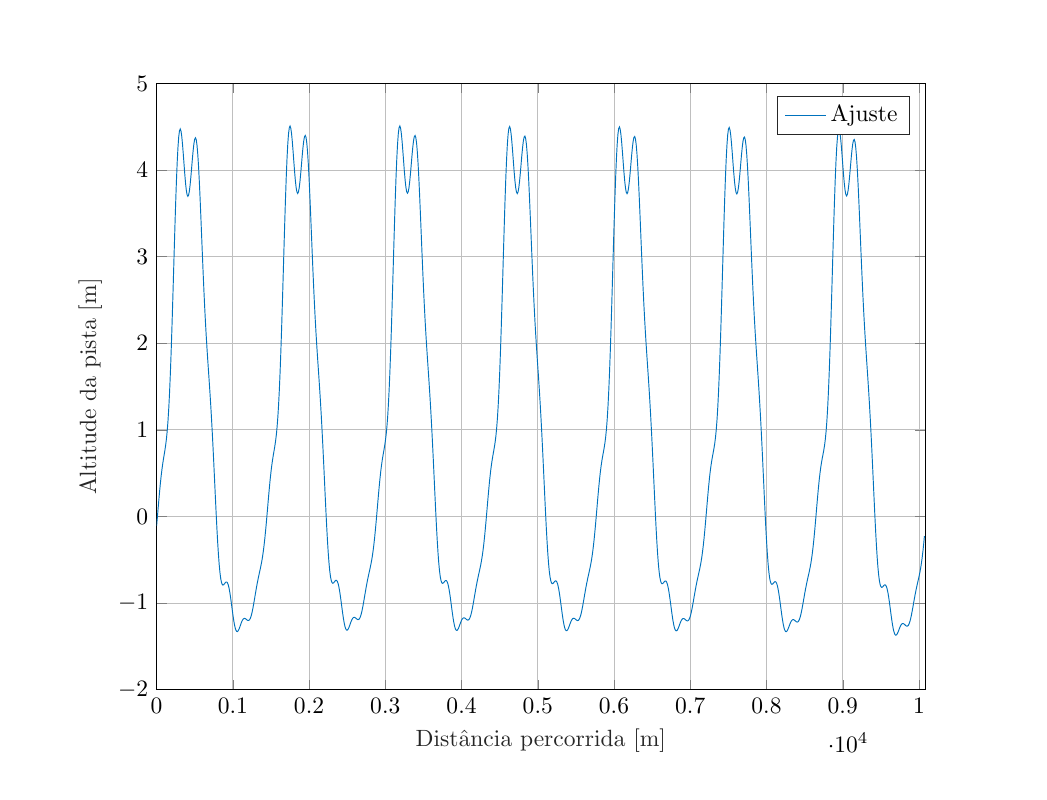
\begin{tikzpicture}[scale=0.85]

\begin{axis}[%
width=4.521in,
height=3.566in,
at={(0.758in,0.481in)},
scale only axis,
xmin=0,
xmax=10080,
xlabel style={font=\color{white!15!black}},
xlabel={Distância percorrida [m]},
ymin=-2,
ymax=5,
ylabel style={font=\color{white!15!black}},
ylabel={Altitude da pista [m]},
axis background/.style={fill=white},
xmajorgrids,
ymajorgrids,
legend style={legend cell align=left, align=left, draw=white!15!black}
]
\addplot [color=mycolor1]
  table[row sep=crcr]{%
1	-0.109711917352081\\
11	-0.00839975833814072\\
21	0.0950935994183011\\
31	0.197575097473076\\
41	0.295906341954157\\
51	0.387379176406482\\
61	0.470078639152616\\
71	0.543194918667103\\
81	0.607248810660309\\
91	0.664201673014787\\
101	0.717430477656014\\
111	0.771560468559376\\
121	0.832161105813\\
131	0.90532420971175\\
141	0.997155276962692\\
151	1.11321865673269\\
161	1.25798366412261\\
171	1.43432106813152\\
181	1.64309736617324\\
191	1.88290788488262\\
201	2.14997946131707\\
211	2.43826005992245\\
221	2.73969727047449\\
231	3.04469152045332\\
241	3.34269442603896\\
251	3.62290937310388\\
261	3.87504138340178\\
271	4.09003753619072\\
281	4.26075828112619\\
291	4.38252407940657\\
301	4.45349069459108\\
311	4.47481944853005\\
321	4.45062481979224\\
331	4.38769956903536\\
341	4.29503563665075\\
351	4.18317584164875\\
361	4.06344547969927\\
371	3.94712305498246\\
381	3.84461469530785\\
391	3.76469681065797\\
401	3.71388623172202\\
411	3.69598683386881\\
421	3.71184736196174\\
431	3.75934802063559\\
441	3.83361482784037\\
451	3.92744231294103\\
461	4.03188842668885\\
471	4.13699192257323\\
481	4.23255310092945\\
491	4.30891444440015\\
501	4.35767864845305\\
511	4.37230773581937\\
521	4.34855776398591\\
531	4.28471812059516\\
541	4.18164127523908\\
551	4.04256664568099\\
561	3.8727594054464\\
571	3.6790001416205\\
581	3.46897299806302\\
591	3.25060734872116\\
601	3.03143056535272\\
611	2.81798693557988\\
621	2.61537055476623\\
631	2.42690877308266\\
641	2.25401858405504\\
651	2.09624249436254\\
661	1.95145434447245\\
671	1.81621068151138\\
681	1.68621091627265\\
691	1.55682067929601\\
701	1.42360824671759\\
711	1.28284396176586\\
721	1.13191714177985\\
731	0.969633539600276\\
741	0.796368175204486\\
751	0.614062149913995\\
761	0.426066616015826\\
771	0.236851065707892\\
781	0.051605264766321\\
791	-0.124226585294145\\
801	-0.28543530967372\\
811	-0.427514275401029\\
821	-0.547062158447048\\
831	-0.642084803994541\\
841	-0.712169858877593\\
851	-0.758519932931108\\
861	-0.783843217554211\\
871	-0.792113527366725\\
881	-0.788223438901982\\
891	-0.777563525199437\\
901	-0.765566810209672\\
911	-0.757259984130101\\
921	-0.756861473257333\\
931	-0.767461349089345\\
941	-0.790809830657308\\
951	-0.827230601643877\\
961	-0.875663350222557\\
971	-0.933827967298308\\
981	-0.998491826252851\\
991	-1.06581252391888\\
1001	-1.13172219610016\\
1011	-1.19231656474594\\
1021	-1.24421244050807\\
1031	-1.28484137061795\\
1041	-1.31265404530945\\
1051	-1.32721924116057\\
1061	-1.32921157058291\\
1071	-1.32029309615128\\
1081	-1.30290391790131\\
1091	-1.27998520033189\\
1101	-1.25466400050152\\
1111	-1.22993216571023\\
1121	-1.20835126193031\\
1131	-1.19181206044295\\
1141	-1.18137094078277\\
1151	-1.17717731518708\\
1161	-1.17849669058402\\
1171	-1.18382421671065\\
1181	-1.19107449731941\\
1191	-1.19782596034705\\
1201	-1.20159292065635\\
1211	-1.20009611694053\\
1221	-1.19150317027772\\
1231	-1.17461400061693\\
1241	-1.14897236222076\\
1251	-1.11489268027755\\
1261	-1.07340046056913\\
1271	-1.02609376840127\\
1281	-0.974941685251106\\
1291	-0.922042386510245\\
1301	-0.869367844030426\\
1311	-0.818523683801552\\
1321	-0.770551248021045\\
1331	-0.725794552227129\\
1341	-0.683848015544151\\
1351	-0.643592252309563\\
1361	-0.603315711498686\\
1371	-0.560910505351947\\
1381	-0.514122357766729\\
1391	-0.460828114779785\\
1401	-0.399310403671038\\
1411	-0.328498261776184\\
1421	-0.248145037368798\\
1431	-0.158920426954973\\
1441	-0.0624016779830519\\
1451	0.0390409958153942\\
1461	0.142458819696212\\
1471	0.244621962609591\\
1481	0.342373910009698\\
1491	0.433009194713195\\
1501	0.514636725900871\\
1511	0.586490261571256\\
1521	0.649150627850389\\
1531	0.70465094198183\\
1541	0.756445837883422\\
1551	0.809237707503833\\
1561	0.868666201312164\\
1571	0.940880473947201\\
1581	1.03202567577401\\
1591	1.14768481484112\\
1601	1.29232337115105\\
1611	1.46878624345062\\
1621	1.67789440831694\\
1631	1.91818212523839\\
1641	2.1858050795613\\
1651	2.4746363321751\\
1661	2.7765514538704\\
1671	3.0818880808922\\
1681	3.38004974341147\\
1691	3.66021056250047\\
1701	3.91206749718755\\
1711	4.12658119495929\\
1721	4.29664574188969\\
1731	4.41763189133126\\
1741	4.48775740399173\\
1751	4.50825126801585\\
1761	4.48329473066804\\
1771	4.41973993115163\\
1781	4.32662498083452\\
1791	4.21452106172837\\
1801	4.09476107417914\\
1811	3.97860935253988\\
1821	3.87643710676308\\
1831	3.79696807207257\\
1841	3.74665334488901\\
1851	3.72922399418815\\
1861	3.7454556265135\\
1871	3.7931618592856\\
1881	3.86741507237606\\
1891	3.96097443033605\\
1901	4.06488454615074\\
1911	4.16919468741892\\
1921	4.26373922867053\\
1931	4.33891587951821\\
1941	4.38639938307744\\
1951	4.3997347376935\\
1961	4.3747649568976\\
1971	4.30986296522801\\
1981	4.20595414475607\\
1991	4.06633382285708\\
2001	3.89630109056\\
2011	3.70264530253945\\
2021	3.49303317666715\\
2031	3.27535163586291\\
2041	3.05706386130738\\
2051	2.84463333293164\\
2061	2.64306324088849\\
2071	2.45558728891871\\
2081	2.28353364450786\\
2091	2.12636792910063\\
2101	1.98190511329033\\
2111	1.84666540848799\\
2121	1.7163370160708\\
2131	1.58629994863694\\
2141	1.45216078056107\\
2151	1.31024842651069\\
2161	1.15802577978455\\
2171	0.994380758508237\\
2181	0.819772148019413\\
2191	0.63621946571085\\
2201	0.447140621642194\\
2211	0.257055072709677\\
2221	0.0711822165349781\\
2231	-0.105026119306842\\
2241	-0.266374844844081\\
2251	-0.408390936247001\\
2261	-0.52772236817059\\
2271	-0.622434877067988\\
2281	-0.692180725667297\\
2291	-0.738225775326999\\
2301	-0.763334352315229\\
2311	-0.771524388431763\\
2321	-0.767716935020035\\
2331	-0.757313347586203\\
2341	-0.745739411463418\\
2351	-0.737997933651879\\
2361	-0.7382697204275\\
2371	-0.749597612541098\\
2381	-0.773679911866189\\
2391	-0.810788934937414\\
2401	-0.859818595970919\\
2411	-0.918452978348607\\
2421	-0.9834369141028\\
2431	-1.05092065765553\\
2441	-1.11684460981355\\
2451	-1.17732724078422\\
2461	-1.22902007508595\\
2471	-1.26939769943262\\
2481	-1.29695778207113\\
2491	-1.31131532379874\\
2501	-1.31318587487361\\
2511	-1.30426321938879\\
2521	-1.28700701334462\\
2531	-1.26436412045858\\
2541	-1.23945315760302\\
2551	-1.21524452852757\\
2561	-1.19426777701328\\
2571	-1.17837453046989\\
2581	-1.1685790351634\\
2591	-1.16498996650145\\
2601	-1.16683768558383\\
2611	-1.17259136664965\\
2621	-1.18015141108624\\
2631	-1.18709518087878\\
2641	-1.19094904643271\\
2651	-1.18945752987899\\
2661	-1.18082112945581\\
2671	-1.163878124775\\
2681	-1.13821188746484\\
2691	-1.10417330744339\\
2701	-1.06281705745925\\
2711	-1.01575962122082\\
2721	-0.964975358495653\\
2731	-0.912553514665536\\
2741	-0.860443314589362\\
2751	-0.810215664323673\\
2761	-0.762868359004461\\
2771	-0.71869720512976\\
2781	-0.677248546929054\\
2791	-0.637360026867475\\
2801	-0.597286881858604\\
2811	-0.554901651476558\\
2821	-0.507946828414134\\
2831	-0.454313597483903\\
2841	-0.392316088042783\\
2851	-0.32092995139631\\
2861	-0.239966711702738\\
2871	-0.150161045476146\\
2881	-0.0531564291649808\\
2891	0.0486153042655554\\
2901	0.152154000824888\\
2911	0.254193570256236\\
2921	0.351560026288614\\
2931	0.441551312851706\\
2941	0.522300934601968\\
2951	0.593086875477846\\
2961	0.654550515125696\\
2971	0.708797066931038\\
2981	0.759358941488504\\
2991	0.811015556340023\\
3001	0.869476400370953\\
3011	0.940947410493913\\
3021	1.03161268752164\\
3031	1.14707310812312\\
3041	1.29178951328604\\
3051	1.46858018988898\\
3061	1.67821998581917\\
3071	1.91918167958509\\
3081	2.18754962831664\\
3091	2.47712207229177\\
3101	2.77970290432061\\
3111	3.08556754338769\\
3121	3.38407219379886\\
3131	3.66436259362606\\
3141	3.91612856605821\\
3151	4.13034521696469\\
3161	4.29994104254356\\
3171	4.42033767516037\\
3181	4.48981521803792\\
3191	4.50967039565048\\
3201	4.48415100883931\\
3211	4.42016809033865\\
3221	4.32680520673144\\
3231	4.21466101621697\\
3241	4.09507504098498\\
3251	3.97929645047824\\
3261	3.87766061455082\\
3271	3.79883782313765\\
3281	3.74921288521327\\
3291	3.73244377411941\\
3301	3.74923295617508\\
3311	3.79732774518316\\
3321	3.87174742517548\\
3331	3.96521654733918\\
3341	4.06876728002307\\
3351	4.17246036019907\\
3361	4.26616516957475\\
3371	4.34033547371321\\
3381	4.38671871661783\\
3391	4.39894329435757\\
3401	4.37293933330678\\
3411	4.3071631763426\\
3421	4.20261273892485\\
3431	4.06263865658181\\
3441	3.89257317190016\\
3451	3.69921354891173\\
3461	3.49020820883375\\
3471	3.27340082063725\\
3481	3.05618971294326\\
3491	2.84495709652224\\
3501	2.64461503596073\\
3511	2.45830362736606\\
3521	2.28726250410126\\
3531	2.1308809180206\\
3541	1.98691565929691\\
3551	1.8518514011584\\
3561	1.72136596576967\\
3571	1.59085453256746\\
3581	1.45596263994659\\
3591	1.31307825849592\\
3601	1.15973811531745\\
3611	0.994912300750151\\
3621	0.819143120439789\\
3631	0.634528032965973\\
3641	0.444551044677242\\
3651	0.253780789344372\\
3661	0.067465453952224\\
3671	-0.108936328528585\\
3681	-0.270244277566914\\
3691	-0.412019541837268\\
3701	-0.530959746561425\\
3711	-0.625190629127377\\
3721	-0.694428927063916\\
3731	-0.740003375712762\\
3741	-0.764733857930665\\
3751	-0.772681697365916\\
3761	-0.768795614412628\\
3771	-0.758486934206376\\
3781	-0.747173456839254\\
3791	-0.739833492203418\\
3801	-0.740609799003622\\
3811	-0.752497782021677\\
3821	-0.777143858212993\\
3831	-0.814769239760178\\
3841	-0.864222532183184\\
3851	-0.923152632602985\\
3861	-0.988282548629893\\
3871	-1.05575593642078\\
3881	-1.12152216306434\\
3891	-1.18172304029534\\
3901	-1.2330452376257\\
3911	-1.27300661210768\\
3921	-1.30015182191712\\
3931	-1.31414188744043\\
3941	-1.31573289867114\\
3951	-1.30664981102404\\
3961	-1.2893711898497\\
3971	-1.26684891960167\\
3981	-1.24219253384207\\
3991	-1.21835044847344\\
4001	-1.1978197932734\\
4011	-1.18241285119381\\
4021	-1.17310174602351\\
4031	-1.16995463817434\\
4041	-1.17216715502379\\
4051	-1.17818305848217\\
4061	-1.18588920790449\\
4071	-1.19286259337564\\
4081	-1.19664230167593\\
4091	-1.19499720194536\\
4101	-1.1861610808664\\
4111	-1.16901079597025\\
4121	-1.14316933894755\\
4131	-1.10902384946087\\
4141	-1.0676577531166\\
4151	-1.02070537634236\\
4161	-0.970145672985785\\
4171	-0.918058229257204\\
4181	-0.866368817033628\\
4191	-0.816613005865686\\
4201	-0.769744574766057\\
4211	-0.726010844066624\\
4221	-0.684910024423064\\
4231	-0.645236952226242\\
4241	-0.605214027510975\\
4251	-0.562694766890764\\
4261	-0.515419104674251\\
4271	-0.461293297230767\\
4281	-0.398663699763548\\
4291	-0.326553224018508\\
4301	-0.244832078074922\\
4311	-0.154300239894579\\
4321	-0.0566675192038929\\
4331	0.0455727546647442\\
4341	0.149369386827174\\
4351	0.251420549341063\\
4361	0.348535438860226\\
4371	0.43801613507362\\
4381	0.518021462428984\\
4391	0.587874283886948\\
4401	0.648277049708184\\
4411	0.701407398116836\\
4421	0.750875621708201\\
4431	0.801538031519352\\
4441	0.859173593767532\\
4451	0.930044467953282\\
4461	1.02037299678602\\
4471	1.13577713279455\\
4481	1.28071227468474\\
4491	1.45796935967078\\
4501	1.66827650581806\\
4511	1.91004460591045\\
4521	2.17928652306115\\
4531	2.46972577130372\\
4541	2.77309491764668\\
4551	3.07960774777241\\
4561	3.37857390822608\\
4571	3.65911164116987\\
4581	3.9109045630591\\
4591	4.12494312733209\\
4601	4.29419101003624\\
4611	4.41412130287145\\
4621	4.48307678853789\\
4631	4.50242198846714\\
4641	4.47647103250519\\
4651	4.41219335336525\\
4661	4.31871725034078\\
4671	4.20666796676953\\
4681	4.0873906626068\\
4691	3.97211834925178\\
4701	3.87114963927479\\
4711	3.79310061457673\\
4721	3.74428925339168\\
4731	3.72830015534106\\
4741	3.74576265609394\\
4751	3.79435806025612\\
4761	3.86905310750416\\
4771	3.96253849399793\\
4781	4.06583484054178\\
4791	4.16901530948211\\
4801	4.26198522019608\\
4811	4.33525521774953\\
4821	4.38064609247041\\
4831	4.39187005086318\\
4841	4.36494447888093\\
4851	4.29840900944683\\
4861	4.1933337038751\\
4871	4.05312389808791\\
4881	3.88314421678459\\
4891	3.69019897482842\\
4901	3.48191742914298\\
4911	3.26609919799272\\
4921	3.05007710428843\\
4931	2.84015163896252\\
4941	2.64114353254819\\
4951	2.45609932428189\\
4961	2.28617041640072\\
4971	2.13067021610322\\
4981	1.98729802936202\\
4991	1.85250379249395\\
5001	1.72195577913788\\
5011	1.59106511764574\\
5021	1.45551697068141\\
5031	1.31175884148751\\
5041	1.15740153965532\\
5051	0.99149732503302\\
5061	0.814671769383148\\
5071	0.629099789858731\\
5081	0.438330822075135\\
5091	0.246981886079804\\
5101	0.0603291160437442\\
5111	-0.116162866917553\\
5121	-0.277329310060742\\
5131	-0.418766089329753\\
5141	-0.537220822197283\\
5151	-0.630879345724785\\
5161	-0.699522720430722\\
5171	-0.744542168499829\\
5181	-0.768812543414552\\
5191	-0.77643783019091\\
5201	-0.772393610273662\\
5211	-0.76210036636017\\
5221	-0.750967170276958\\
5231	-0.743947226880766\\
5241	-0.745144827455544\\
5251	-0.757507744184746\\
5261	-0.782630549922456\\
5271	-0.820683622954029\\
5281	-0.870470731289588\\
5291	-0.929606210591703\\
5301	-0.99479196170474\\
5311	-1.06216578441959\\
5321	-1.12768670827949\\
5331	-1.18752047223153\\
5341	-1.23838931245838\\
5351	-1.27785457667711\\
5361	-1.30450791418447\\
5371	-1.31805615030916\\
5381	-1.31929550819321\\
5391	-1.30998155813075\\
5401	-1.29261112467127\\
5411	-1.27014043391958\\
5421	-1.24566929528688\\
5431	-1.22212359738301\\
5441	-1.20196767103155\\
5451	-1.18697426226862\\
5461	-1.17807339173284\\
5471	-1.17529293472056\\
5481	-1.17779420370248\\
5491	-1.18399611608134\\
5501	-1.19177265158176\\
5511	-1.19870112164413\\
5521	-1.20233398658379\\
5531	-1.20046501983181\\
5541	-1.19136169939746\\
5551	-1.17393966917773\\
5561	-1.14786153323961\\
5571	-1.11355045593862\\
5581	-1.07211819273916\\
5591	-1.02521633013662\\
5601	-0.974827727368291\\
5611	-0.923021580649208\\
5621	-0.871699504103512\\
5631	-0.822361118090603\\
5641	-0.775915722528825\\
5651	-0.732561882075727\\
5661	-0.691749623454086\\
5671	-0.65223115090478\\
5681	-0.612196409817006\\
5691	-0.569480448737413\\
5701	-0.521821319121635\\
5711	-0.467141081524286\\
5721	-0.403819037629839\\
5731	-0.330926000139338\\
5741	-0.248391360738889\\
5751	-0.157080710186729\\
5761	-0.0587702847557871\\
5771	0.0439852237341798\\
5781	0.148083927953945\\
5791	0.250188792131437\\
5801	0.347092856381779\\
5811	0.436103063773211\\
5821	0.515404282722282\\
5831	0.584364905130815\\
5841	0.643748963145229\\
5851	0.695806840655715\\
5861	0.744226808470209\\
5871	0.793941929590395\\
5881	0.850800277683937\\
5891	0.921119667893307\\
5901	1.011159971315\\
5911	1.12655542147619\\
5921	1.271755172588\\
5931	1.44952207862169\\
5941	1.66053693379028\\
5951	1.90314834984942\\
5961	2.17329754111752\\
5971	2.46463340145052\\
5981	2.76881753564511\\
5991	3.07600269022259\\
6001	3.37545273019981\\
6011	3.656259294355\\
6021	3.9081007238689\\
6031	4.12198370809991\\
6041	4.29090786883547\\
6051	4.41039833106196\\
6061	4.47886088571468\\
6071	4.49772790263973\\
6081	4.471379606938\\
6091	4.40684332952534\\
6101	4.31329137350302\\
6111	4.20137467243125\\
6121	4.08244303908869\\
6131	3.96771233603063\\
6141	3.8674435067867\\
6151	3.79019767061393\\
6161	3.74222544191348\\
6171	3.72703777993521\\
6181	3.74519091099121\\
6191	3.79430043593274\\
6201	3.86928111097238\\
6211	3.96279054259811\\
6221	4.06583870523537\\
6231	4.16851214344749\\
6241	4.26075304238937\\
6251	4.3331297448767\\
6261	4.37753702534393\\
6271	4.38777130422695\\
6281	4.35993736394961\\
6291	4.29265798971039\\
6301	4.1870749929942\\
6311	4.04664779638075\\
6321	3.87677263408077\\
6331	3.68426001332165\\
6341	3.47671916247087\\
6351	3.26190485882661\\
6361	3.04708377558004\\
6371	2.83847424421572\\
6381	2.6408054648315\\
6391	2.45703048271724\\
6401	2.28821278321631\\
6411	2.13359046321988\\
6421	1.99080604758482\\
6431	1.85627554080943\\
6441	1.72565849925616\\
6451	1.59438277965339\\
6461	1.45817382375786\\
6471	1.31353913658475\\
6481	1.15816384991459\\
6491	0.991182380977039\\
6501	0.813303304567194\\
6511	0.626778506348153\\
6521	0.4352221789461\\
6531	0.243298935633004\\
6541	0.0563120162181395\\
6551	-0.120268783558876\\
6561	-0.281294950527896\\
6571	-0.42239763380241\\
6581	-0.540374774359932\\
6591	-0.633472396556515\\
6601	-0.70153572122028\\
6611	-0.746018060524634\\
6621	-0.769848644848614\\
6631	-0.77717338488352\\
6641	-0.77299391283215\\
6651	-0.762739057602265\\
6661	-0.751808423263048\\
6671	-0.745129507602381\\
6681	-0.746767722214123\\
6691	-0.759623018490201\\
6701	-0.785238174383896\\
6711	-0.823733012168367\\
6721	-0.87386693919754\\
6731	-0.93322035773951\\
6741	-0.998474779967866\\
6751	-1.06576288867175\\
6761	-1.13105406663915\\
6771	-1.19053855787688\\
6781	-1.24097457724413\\
6791	-1.27996717273519\\
6801	-1.30615497509042\\
6811	-1.31929038980985\\
6821	-1.32020935804754\\
6831	-1.31069750224054\\
6841	-1.29326925241673\\
6851	-1.27088449661721\\
6861	-1.24663268151009\\
6871	-1.22341663376531\\
6881	-1.20366750708417\\
6891	-1.18911832614556\\
6901	-1.18065703615198\\
6911	-1.17827146502713\\
6921	-1.18108903564423\\
6931	-1.18750439313141\\
6941	-1.19537930179836\\
6951	-1.20229208664139\\
6961	-1.20580923474658\\
6971	-1.20374997459447\\
6981	-1.19441586979588\\
6991	-1.17676154907852\\
7001	-1.15048921068425\\
7011	-1.1160578084506\\
7021	-1.07460699575215\\
7031	-1.02780502950524\\
7041	-0.977637981160131\\
7051	-0.926163924454248\\
7061	-0.875259612208226\\
7071	-0.826388106781589\\
7081	-0.780413772084764\\
7091	-0.737486155146442\\
7101	-0.697007056617631\\
7111	-0.657686230503229\\
7121	-0.617681556658883\\
7131	-0.574810175445773\\
7141	-0.526808933487088\\
7151	-0.471616427767162\\
7161	-0.407645623721687\\
7171	-0.334015869348012\\
7181	-0.250716231079849\\
7191	-0.158678213566937\\
7201	-0.0597445617627375\\
7211	0.0434688150042029\\
7221	0.147809695550517\\
7231	0.249906374477391\\
7241	0.346536401770879\\
7251	0.435012314442613\\
7261	0.513545748882924\\
7271	0.58155127266305\\
7281	0.639855005254393\\
7291	0.690780389188819\\
7301	0.738093760638044\\
7311	0.786804783693372\\
7321	0.842830260918894\\
7331	0.912543089050261\\
7341	1.00223994928583\\
7351	1.11757055938818\\
7361	1.26297702811862\\
7371	1.44119339704165\\
7381	1.65285254976734\\
7391	1.89624043131084\\
7401	2.16722646355438\\
7411	2.45938503801703\\
7421	2.76430717231811\\
7431	3.07208517813766\\
7441	3.37193792328874\\
7451	3.6529313410688\\
7461	3.90473943112655\\
7471	4.11838600618794\\
7481	4.28690739578024\\
7491	4.40588132572593\\
7501	4.47377691574696\\
7511	4.49209442642569\\
7521	4.46527993526424\\
7531	4.400418161491\\
7541	4.30672467685665\\
7551	4.19487520652659\\
7561	4.07622323047485\\
7571	3.9619664741243\\
7581	3.86232730580276\\
7591	3.78581113579335\\
7601	3.73860069188631\\
7611	3.72413303781792\\
7621	3.74289132358689\\
7631	3.79242576274579\\
7641	3.86759969829595\\
7651	3.96103841935221\\
7661	4.06374215910588\\
7671	4.16581180191836\\
7681	4.25722732434861\\
7691	4.3286155798219\\
7701	4.37194595695006\\
7711	4.38109948435756\\
7721	4.35226846800225\\
7731	4.2841586981622\\
7741	4.17798333274786\\
7751	4.03725526139993\\
7761	3.86740155221951\\
7771	3.67523804653447\\
7781	3.46835308341198\\
7791	3.25445581554871\\
7801	3.04074613164843\\
7811	2.83335977527225\\
7821	2.63693423183279\\
7831	2.45432912774566\\
7841	2.28652035687543\\
7851	2.13267124948148\\
7861	1.99036825914209\\
7871	1.85599426732478\\
7881	1.72520094479848\\
7891	1.59343365339373\\
7901	1.45645876325882\\
7911	1.31084424261564\\
7921	1.15434977611166\\
7931	0.986191916808387\\
7941	0.807161970594909\\
7951	0.619588294202077\\
7961	0.427149159872773\\
7971	0.234555978707817\\
7981	0.0471382553501445\\
7991	-0.129629849521732\\
8001	-0.290616767448686\\
8011	-0.431489457692471\\
8021	-0.549096505539075\\
8031	-0.64174419916296\\
8041	-0.709341746213374\\
8051	-0.753404142381356\\
8061	-0.776914393574985\\
8071	-0.78405959540548\\
8081	-0.779866618407227\\
8091	-0.769771827220102\\
8101	-0.759164622340435\\
8111	-0.752946198467872\\
8121	-0.755142682906191\\
8131	-0.768606026551919\\
8141	-0.794827270057781\\
8151	-0.833875964981332\\
8161	-0.884467640493358\\
8171	-0.944149396724428\\
8181	-1.00958307563319\\
8191	-1.07689697975942\\
8201	-1.14207153047971\\
8211	-1.20132204683009\\
8221	-1.25144312467191\\
8231	-1.29008371120361\\
8241	-1.3159293981306\\
8251	-1.32877793633509\\
8261	-1.32950456143636\\
8271	-1.31992437914831\\
8281	-1.30256876786739\\
8291	-1.2804005974098\\
8301	-1.25649831553355\\
8311	-1.23374115727839\\
8321	-1.21452672796891\\
8331	-1.20054815460003\\
8341	-1.19265134310186\\
8351	-1.19078431965754\\
8361	-1.19404104934135\\
8371	-1.20079248162257\\
8381	-1.20888883138123\\
8391	-1.21591012826711\\
8401	-1.21943753540864\\
8411	-1.21731628054999\\
8421	-1.20788239857789\\
8431	-1.19012969157679\\
8441	-1.16379992332827\\
8451	-1.12938759190208\\
8461	-1.08805980784403\\
8471	-1.04150090203569\\
8481	-0.991699460684102\\
8491	-0.940701701124891\\
8501	-0.890358812759513\\
8511	-0.842096695216966\\
8521	-0.796734325721692\\
8531	-0.754371979419795\\
8541	-0.714363197083409\\
8551	-0.675375472459833\\
8561	-0.635535015902263\\
8571	-0.59264162446658\\
8581	-0.544431620444267\\
8591	-0.488860869090527\\
8601	-0.42437671347977\\
8611	-0.350147665068909\\
8621	-0.266222947654343\\
8631	-0.173600270670087\\
8641	-0.0741889588387081\\
8651	0.029334016950841\\
8661	0.133766470226962\\
8671	0.235702572313187\\
8681	0.331905055122274\\
8691	0.419692782874768\\
8701	0.497304883520215\\
8711	0.564202743597134\\
8721	0.62127506928774\\
8731	0.670918666695638\\
8741	0.716978015286696\\
8751	0.764539219899451\\
8761	0.819587424681491\\
8771	0.888550026756298\\
8781	0.977759794334847\\
8791	1.09288113073782\\
8801	1.23834829957129\\
8811	1.41686580522804\\
8821	1.62901804120995\\
8831	1.87302790960728\\
8841	2.14469290726212\\
8851	2.43751305283213\\
8861	2.74300916305842\\
8871	3.05121372906064\\
8881	3.35130141361612\\
8891	3.63231334755117\\
8901	3.88392012472716\\
8911	4.0971635675009\\
8921	4.26511747098089\\
8931	4.38341272272904\\
8941	4.45058208338723\\
8951	4.46819373728526\\
8961	4.44075936223278\\
8971	4.37542054766766\\
8981	4.28143539250787\\
8991	4.16950351116048\\
9001	4.05098106444816\\
9011	3.9370466548522\\
9021	3.8378831748886\\
9031	3.76193958774887\\
9041	3.71533022204889\\
9051	3.70141800223998\\
9061	3.72061304662164\\
9071	3.77040050869587\\
9081	3.84559289760919\\
9091	3.93878396405898\\
9101	4.04096510882081\\
9111	4.1422525140611\\
9121	4.23266487057928\\
9131	4.30288834959105\\
9141	4.34496757598024\\
9151	4.35286857134679\\
9161	4.32287128222323\\
9171	4.25376434719113\\
9181	4.14683185865955\\
9191	4.00563954778157\\
9201	3.8356445378355\\
9211	3.64366714612535\\
9221	3.43727396512377\\
9231	3.22412774583121\\
9241	3.0113609668279\\
9251	2.80502636626579\\
9261	2.60966954257118\\
9271	2.42805679028131\\
9281	2.26107674811657\\
9291	2.10781853241108\\
9301	1.96581324173337\\
9311	1.83141144666797\\
9321	1.70025776416936\\
9331	1.56781583483287\\
9341	1.42989360066487\\
9351	1.28311994656556\\
9361	1.12532933146248\\
9371	0.955820413072912\\
9381	0.775466947419435\\
9391	0.586673257344062\\
9401	0.393181012063504\\
9411	0.199747622672146\\
9421	0.0117280184922139\\
9431	-0.165400080810512\\
9441	-0.326522750100184\\
9451	-0.467343286995707\\
9461	-0.584761231633036\\
9471	-0.677143201659642\\
9481	-0.744462207517106\\
9491	-0.78829451263121\\
9501	-0.811676289767742\\
9511	-0.818835073994697\\
9521	-0.814822159982188\\
9531	-0.805080638858982\\
9541	-0.794988975757328\\
9551	-0.7894214726074\\
9561	-0.792364575784742\\
9571	-0.806622064732274\\
9581	-0.833633309021319\\
9591	-0.873417882386367\\
9601	-0.924647924063045\\
9611	-0.984837866629531\\
9621	-1.05063060077145\\
9631	-1.11815078304702\\
9641	-1.18339055345956\\
9651	-1.2425908683301\\
9661	-1.2925830973638\\
9671	-1.33106027543809\\
9681	-1.35675492421612\\
9691	-1.36950989546535\\
9701	-1.37023928765588\\
9711	-1.36078711515073\\
9721	-1.34370104459822\\
9731	-1.32194624736828\\
9741	-1.29858953894479\\
9751	-1.27648603836314\\
9761	-1.25799943856238\\
9771	-1.24478280093972\\
9781	-1.23764003702797\\
9791	-1.23647962501759\\
9801	-1.24036251066657\\
9811	-1.24763652895464\\
9821	-1.25614101324343\\
9831	-1.26345838798365\\
9841	-1.26718513781449\\
9851	-1.26519302759362\\
9861	-1.25585294076593\\
9871	-1.23819803160341\\
9881	-1.21200959064062\\
9891	-1.17781740521239\\
9901	-1.13681559386255\\
9911	-1.09070395855907\\
9921	-1.04147289893599\\
9931	-0.991156040975843\\
9941	-0.941578310392307\\
9951	-0.894127843829391\\
9961	-0.849577787757336\\
9971	-0.80797889922967\\
9981	-0.768636433971275\\
9991	-0.730175823784505\\
10001	-0.690692012705508\\
10011	-0.647968024570274\\
10021	-0.599740340505644\\
10031	-0.543982825652031\\
10041	-0.479177911405949\\
10051	-0.40454389486101\\
10061	-0.32019063148132\\
10071	-0.227182316423454\\
};
\addlegendentry{Ajuste}

%\addlegendentry{Termino da volta}

\end{axis}

\begin{axis}[%
width=5.833in,
height=4.375in,
at={(0in,0in)},
scale only axis,
xmin=0,
xmax=1,
ymin=0,
ymax=1,
axis line style={draw=none},
ticks=none,
axis x line*=bottom,
axis y line*=left
]
\end{axis}
\end{tikzpicture}%
%     \label{graf:pista_voltas}
%     \caption*{\footnotesize{Fonte: Elaborada pelo autor.}}
% \end{figure}

\section{estratégia de pista ótima}
\label{sec:resultados_otimo}
 
O código desenvolvido, conforme descrito na Seção \ref{sec:OCPporposto}, para solução o problema de controle ótimo proposto na Equação 
(\ref{eq:ObjOCP_final}) gerou um problema de programação não linear com 3005 variáveis de otimização.
Foram gastos para a execução de todo o programa $\sim 14.4$ segundos onde $\sim 7,2$ segundos deste foram utilizados na otimização do NLP em $636$ iterações da biblioteca IPOP e reposta não violou nenhuma das restrições. 
A sequência de controle ótima de $i$ e os estados gerados por ela $x$ e $v$ estão apresentados nos gráficos da Figura \ref{graf:resultadoOCP}. 
Os parâmetros otimizados tempo final $T$ e raio do eixo do motor $r_m$ são exibidos na Tabela \ref{tab:resultadoOCP} junto das métricas marca, velocidade media e velocidade final. 

\begin{table}[h]
	\centering
	\caption{Parâmetros otimizados e métricas da estratégia ótima}
	\rowcolors{1}{}{lightgray}
	\begin{tabular}{lll}
		\toprule
		\textbf{Constante} & \textbf{Unidade} & \textbf{Valor}\\
		\hline
		Marca                               & [$km/kWh$]   & 905.68  \\
        Raio do eixo do motor               & [$mm$]       & 27.56   \\
        Tempo total de prova                & [$s$]        & 1400.0  \\  
        Velocidade média                    & [$km/h$]     & 25.92   \\
        Velocidade final                    & [$km/h$ ]    & 17.09   \\
		\bottomrule
	\end{tabular}
	\caption*{\footnotesize Fonte: Elaborada pelo autor.}
	\label{tab:resultadoOCP}
\end{table}

\begin{figure}[H]
    \centering
    \caption{sequência de controle ótima $i$ e estados $v$ e $x$ correspondentes}
    % This file was created by matlab2tikz.
%
%The latest updates can be retrieved from
%  http://www.mathworks.com/matlabcentral/fileexchange/22022-matlab2tikz-matlab2tikz
%where you can also make suggestions and rate matlab2tikz.
%
\definecolor{mycolor1}{rgb}{0.00000,0.44700,0.74100}%
%
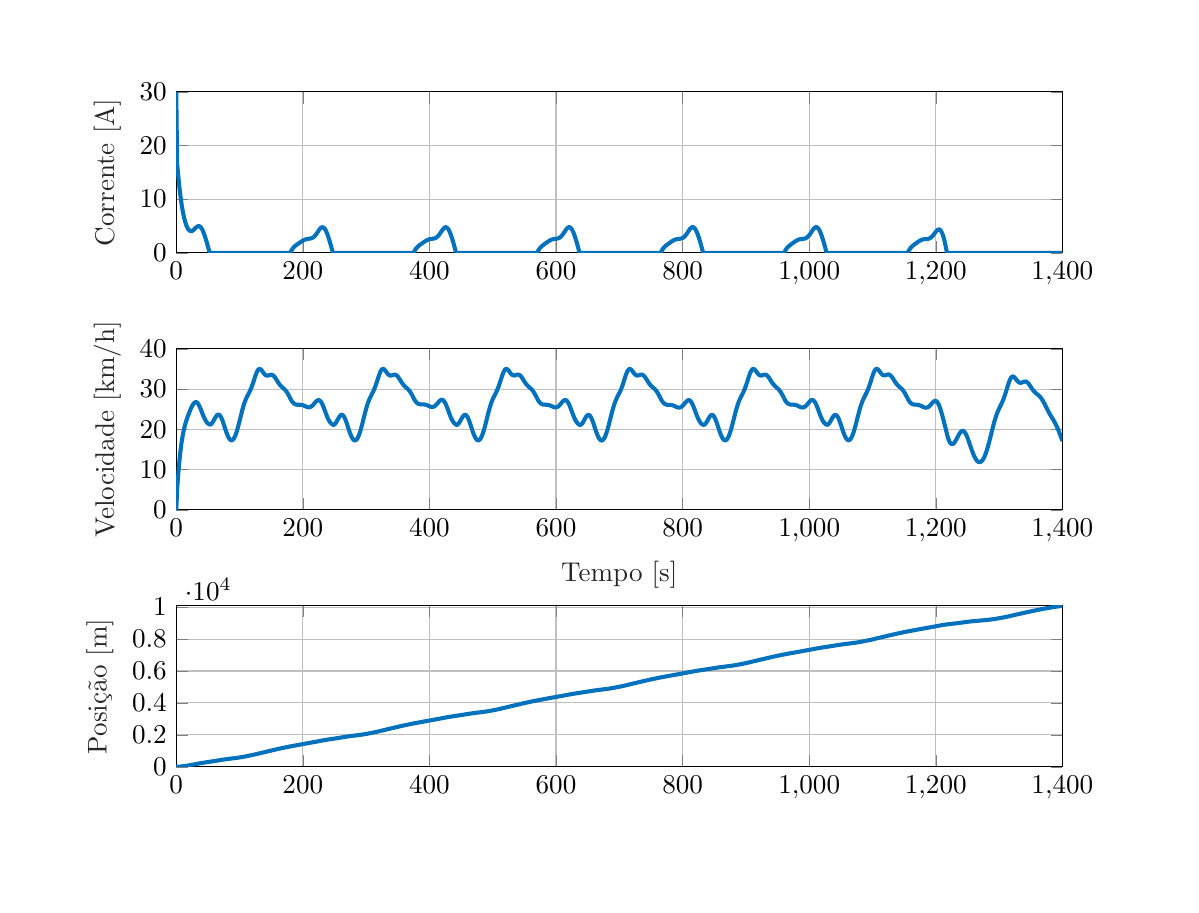
\begin{tikzpicture}[scale=0.98]

\begin{axis}[%
width=4.521in,
height=0.821in,
at={(0.758in,3.226in)},
scale only axis,
xmin=0,
xmax=1400,
ymin=0,
ymax=30,
ylabel style={font=\color{white!15!black}},
ylabel={Corrente [A]},
axis background/.style={fill=white},
xmajorgrids,
ymajorgrids
]
\addplot [color=mycolor1, line width=1.5pt, forget plot]
  table[row sep=crcr]{%
0	30\\
1.4	16.5908716133211\\
2.8	14.7975933021474\\
4.2	13.137184788085\\
5.6	11.6325501085416\\
7	10.2920883505672\\
8.4	9.11422332586441\\
9.8	8.09114984219666\\
11.2	7.21175288843701\\
12.6	6.46375587985035\\
14	5.8351940719724\\
15.4	5.31531669300007\\
16.8	4.89501386468417\\
18.2	4.5668515157771\\
19.6	4.32478438224807\\
21	4.16360788306743\\
22.4	4.07820863661113\\
23.8	4.0626849467355\\
25.2	4.10943453585793\\
26.6	4.20834319463988\\
28	4.34624244593825\\
29.4	4.50681581938552\\
30.8	4.67109756354158\\
32.2	4.81860877547889\\
33.6	4.92902235787828\\
35	4.98408199622832\\
36.4	4.96938793546667\\
37.8	4.87566277485428\\
39.2	4.69923774427305\\
40.6	4.44170805040274\\
42	4.10891232863754\\
43.4	3.70952230451787\\
44.8	3.25355442203563\\
46.2	2.75105291368079\\
47.6	2.21108727815738\\
49	1.64110000799875\\
50.4	1.04655996790471\\
51.8	0.430828806482503\\
53.2	2.49850266737891e-06\\
54.6	5.90910953503015e-07\\
56	3.31726220863511e-07\\
57.4	2.30632062336436e-07\\
58.8	1.77778784848997e-07\\
60.2	1.45966363670605e-07\\
61.6	1.25219764266451e-07\\
63	1.1099968354376e-07\\
64.4	1.00913246487559e-07\\
65.8	9.35400834569873e-08\\
67.2	8.79418484091781e-08\\
68.6	8.34384732078637e-08\\
70	7.95072542669334e-08\\
71.4	7.57462744259439e-08\\
72.8	7.18706320220775e-08\\
74.2	6.7717760883009e-08\\
75.6	6.32435423539649e-08\\
77	5.85006880932302e-08\\
78.4	5.36029356704401e-08\\
79.8	4.86862975009238e-08\\
81.2	4.38782736341266e-08\\
82.6	3.92801371577486e-08\\
84	3.49613414096772e-08\\
85.4	3.09619488540489e-08\\
86.8	2.72987704798224e-08\\
88.2	2.39721761005805e-08\\
89.6	2.09719965566549e-08\\
91	1.82819935223205e-08\\
92.4	1.58829453549563e-08\\
93.8	1.37546227495376e-08\\
95.2	1.18769614437883e-08\\
96.6	1.02306907827426e-08\\
98	8.79760744972617e-09\\
99.4	7.56062045368596e-09\\
100.8	6.5036456600661e-09\\
102.2	5.61139679657194e-09\\
103.6	4.86910335793632e-09\\
105	4.26218229489704e-09\\
106.4	3.77589805924489e-09\\
107.8	3.39506209059567e-09\\
109.2	3.10384364404295e-09\\
110.6	2.88578086528639e-09\\
112	2.72408224481862e-09\\
113.4	2.60228055972356e-09\\
114.8	2.50523539412068e-09\\
116.2	2.4203813628584e-09\\
117.6	2.3390130482772e-09\\
119	2.25732764382615e-09\\
120.4	2.17695441264327e-09\\
121.8	2.10479984318971e-09\\
123.2	2.05219725216288e-09\\
124.6	2.03350452338571e-09\\
126	2.06438184925517e-09\\
127.4	2.15998042952392e-09\\
128.8	2.33321034815482e-09\\
130.2	2.59318776079313e-09\\
131.6	3.31799460434381e-09\\
133	5.10208000250258e-09\\
134.4	5.77290747752772e-09\\
135.8	6.53202756336531e-09\\
137.2	7.36018163168841e-09\\
138.6	8.23622589345305e-09\\
140	9.14135748394564e-09\\
141.4	1.00637097711035e-08\\
142.8	1.1002318246778e-08\\
144.2	1.1969566219922e-08\\
145.6	1.29916792575458e-08\\
147	1.41074231092653e-08\\
148.4	1.53655880416358e-08\\
149.8	1.68219596856432e-08\\
151.2	1.85363309890866e-08\\
152.6	2.05698794289482e-08\\
154	2.29831016203149e-08\\
155.4	2.58345695731213e-08\\
156.8	2.9181054647704e-08\\
158.2	3.30799739533824e-08\\
159.6	3.75955098631008e-08\\
161	4.28100096539943e-08\\
162.4	4.88424045222559e-08\\
163.8	5.58757189381499e-08\\
165.2	6.41970438066863e-08\\
166.6	7.42569758067376e-08\\
168	8.67638906738694e-08\\
169.4	1.02846782285864e-07\\
170.8	1.24362735296327e-07\\
172.2	1.54533424393758e-07\\
173.6	1.99412198597069e-07\\
175	2.71785143634952e-07\\
176.4	4.03975030355348e-07\\
177.8	7.07658616835562e-07\\
179.2	1.9984390767144e-06\\
180.6	0.133779312521265\\
182	0.45461926046747\\
183.4	0.717531799543894\\
184.8	0.933500503494147\\
186.2	1.11285381733365\\
187.6	1.26511240662139\\
189	1.39873128969253\\
190.4	1.52082121451857\\
191.8	1.63689942704443\\
193.2	1.75070910566254\\
194.6	1.86414362137784\\
196	1.97730858682545\\
197.4	2.08874564011453\\
198.8	2.19582355239522\\
200.2	2.29527504206337\\
201.6	2.38382700493686\\
203	2.45884674021652\\
204.4	2.51891627574799\\
205.8	2.56425588392216\\
207.2	2.59694402101899\\
208.6	2.62091540695402\\
210	2.6417503850725\\
211.4	2.66628809214885\\
212.8	2.70210030976688\\
214.2	2.75685573005365\\
215.6	2.83759402545968\\
217	2.94992544767176\\
218.4	3.09718298258586\\
219.8	3.27958408970979\\
221.2	3.49350417656519\\
222.6	3.73101114927481\\
224	3.97983711814161\\
225.4	4.22394246412469\\
226.8	4.44473892681835\\
228.2	4.62288578694005\\
229.6	4.74039604461681\\
231	4.78265675037943\\
232.4	4.73994682451026\\
233.8	4.60815130888152\\
235.2	4.38858327615256\\
236.6	4.08704874163103\\
238	3.71244326630671\\
239.4	3.27521200870653\\
240.8	2.78595025031031\\
242.2	2.25431174617877\\
243.6	1.68828519259058\\
245	1.09378298345786\\
246.4	0.474486238023902\\
247.8	3.04589800976699e-06\\
249.2	6.09250982552053e-07\\
250.6	3.33961712444779e-07\\
252	2.29541831213582e-07\\
253.4	1.75554385417239e-07\\
254.8	1.4322613442492e-07\\
256.2	1.22186875284483e-07\\
257.6	1.07772065975249e-07\\
259	9.7548440326809e-08\\
260.4	9.0088938174608e-08\\
261.8	8.44641296673402e-08\\
263.2	8.00092079543124e-08\\
264.6	7.6215584351143e-08\\
266	7.2687179108179e-08\\
267.4	6.91313101462222e-08\\
268.8	6.53629100959592e-08\\
270.2	6.13049432662931e-08\\
271.6	5.69748412569785e-08\\
273	5.24567690734282e-08\\
274.4	4.78676861842771e-08\\
275.8	4.3327177931792e-08\\
277.2	3.89373858953255e-08\\
278.6	3.47740086685065e-08\\
280	3.0885695672841e-08\\
281.4	2.72981093892216e-08\\
282.8	2.40196040706769e-08\\
284.2	2.10466799273623e-08\\
285.6	1.83684069466384e-08\\
287	1.59696575749673e-08\\
288.4	1.38332951662644e-08\\
289.8	1.19415604901134e-08\\
291.2	1.02768882596809e-08\\
292.6	8.8223363633962e-09\\
294	7.56175639333105e-09\\
295.4	6.47978925528848e-09\\
296.8	5.56173813671093e-09\\
298.2	4.79335285440425e-09\\
299.6	4.16055347094234e-09\\
301	3.64912577325855e-09\\
302.4	3.24443492969808e-09\\
303.8	2.93122281972444e-09\\
305.2	2.69357243429996e-09\\
306.6	2.51512880682548e-09\\
308	2.37964721489313e-09\\
309.4	2.27188551266111e-09\\
310.8	2.17876883246456e-09\\
312.2	2.09065068912739e-09\\
313.6	2.00241292627514e-09\\
315	1.91413130155462e-09\\
316.4	1.83110690267217e-09\\
317.8	1.76320787388986e-09\\
319.2	1.72362453531847e-09\\
320.6	1.72724919088908e-09\\
322	1.78891500082788e-09\\
323.4	1.92167985596474e-09\\
324.8	2.13527078583048e-09\\
326.2	2.90284438631733e-09\\
327.6	5.02088119042007e-09\\
329	5.6673097132313e-09\\
330.4	6.40757000303049e-09\\
331.8	7.22340978297131e-09\\
333.2	8.09365311605892e-09\\
334.6	8.99820567591893e-09\\
336	9.92268420432135e-09\\
337.4	1.08627031577149e-08\\
338.8	1.18268457422695e-08\\
340.2	1.2837727251235e-08\\
341.6	1.39311459972738e-08\\
343	1.51538189843146e-08\\
344.4	1.65604091302896e-08\\
345.8	1.82104626139331e-08\\
347.2	2.01656451064479e-08\\
348.6	2.24874898932264e-08\\
350	2.52358829494867e-08\\
351.4	2.84687436963277e-08\\
352.8	3.2243754298916e-08\\
354.2	3.66234145104835e-08\\
355.6	4.16850105766907e-08\\
357	4.75372463661087e-08\\
358.4	5.43455231680576e-08\\
359.8	6.23688292843613e-08\\
361.2	7.20141271273717e-08\\
362.6	8.3921116695988e-08\\
364	9.91056711492713e-08\\
365.4	1.19225220479613e-07\\
366.8	1.47116563389775e-07\\
368.2	1.88003809404299e-07\\
369.6	2.5259773429486e-07\\
371	3.66728448051209e-07\\
372.4	6.1217374413105e-07\\
373.8	1.45412551532305e-06\\
375.2	0.0544616563394439\\
376.6	0.389058476548115\\
378	0.663427595189136\\
379.4	0.88862592150463\\
380.8	1.07511813666937\\
382.2	1.23261708097234\\
383.6	1.36983457599853\\
385	1.49419599541166\\
386.4	1.61157467802551\\
387.8	1.72608799797707\\
389.2	1.83999280171887\\
390.6	1.95371510253595\\
392	2.0660412339276\\
393.4	2.17448086182593\\
394.8	2.27578587111939\\
396.2	2.36657771769693\\
397.6	2.44400813731039\\
399	2.50636386009773\\
400.4	2.55353133210854\\
401.8	2.58726149050353\\
403.2	2.61120932653211\\
404.6	2.63075662853373\\
406	2.65264884924266\\
407.4	2.68448410557929\\
408.8	2.73408642957011\\
410.2	2.80878442737289\\
411.6	2.91461061897346\\
413	3.05544500620009\\
414.4	3.23215377693638\\
415.8	3.44181838234689\\
417.2	3.67719992883998\\
418.6	3.92661723642737\\
420	4.17440615768661\\
421.4	4.402049614892\\
422.8	4.58992058082244\\
424.2	4.71939807484035\\
425.6	4.77496695662089\\
427	4.74586874936915\\
428.4	4.62696815061933\\
429.8	4.41870703459565\\
431.2	4.12625202008701\\
432.6	3.75811414125866\\
434	3.32457956904992\\
435.4	2.83624537480508\\
436.8	2.30286534184352\\
438.2	1.73254371785082\\
439.6	1.13124633817054\\
441	0.502694765888325\\
442.4	3.37691071173289e-06\\
443.8	6.10369508317374e-07\\
445.2	3.30222017302175e-07\\
446.6	2.25465994315507e-07\\
448	1.71594441411919e-07\\
449.4	1.39403337881065e-07\\
450.8	1.18458999037717e-07\\
452.2	1.04095662888392e-07\\
453.6	9.38925594568533e-08\\
455	8.64394748288426e-08\\
456.4	8.08261938051766e-08\\
457.8	7.64082509305615e-08\\
459.2	7.26962037603037e-08\\
460.6	6.93083115006558e-08\\
462	6.59575162437451e-08\\
463.4	6.24532880988578e-08\\
464.8	5.87028077205792e-08\\
466.2	5.47014110687277e-08\\
467.6	5.05104273468256e-08\\
469	4.62280209698495e-08\\
470.4	4.19614942211364e-08\\
471.8	3.7807303239557e-08\\
473.2	3.3840645842364e-08\\
474.6	3.01129770873694e-08\\
476	2.6654412562741e-08\\
477.4	2.34782337261635e-08\\
478.8	2.0585646898192e-08\\
480.2	1.79698705922316e-08\\
481.6	1.56192591028304e-08\\
483	1.35195068931532e-08\\
484.4	1.16551091095137e-08\\
485.8	1.00102715926581e-08\\
487.2	8.56943342312294e-09\\
488.6	7.31752219215076e-09\\
490	6.24002339916211e-09\\
491.4	5.32291664631715e-09\\
492.8	4.55251388311405e-09\\
494.2	3.91522846738483e-09\\
495.6	3.39730740964527e-09\\
497	2.9845713927923e-09\\
498.4	2.66222491345512e-09\\
499.8	2.41481613427488e-09\\
501.2	2.22643305237729e-09\\
502.6	2.08120713300873e-09\\
504	1.96414718821511e-09\\
505.4	1.86224397677954e-09\\
506.8	1.76568604084564e-09\\
508.2	1.66894469438499e-09\\
509.6	1.57146290055161e-09\\
511	1.47774450846858e-09\\
512.4	1.39677432524613e-09\\
513.8	1.34085451179903e-09\\
515.2	1.32405554600087e-09\\
516.6	1.36051231024553e-09\\
518	1.46275543208431e-09\\
519.4	1.64019961460953e-09\\
520.8	1.96210610138229e-09\\
522.2	3.00348499029203e-09\\
523.6	5.31131752744726e-09\\
525	6.02068146678872e-09\\
526.4	6.80600601783905e-09\\
527.8	7.64665780424888e-09\\
529.2	8.52251979747801e-09\\
530.6	9.41846541561835e-09\\
532	1.03286155356136e-08\\
533.4	1.12594114078447e-08\\
534.8	1.22308644633404e-08\\
536.2	1.32759040020553e-08\\
537.6	1.44382565792911e-08\\
539	1.57695368355097e-08\\
540.4	1.7326177129401e-08\\
541.8	1.9166609608172e-08\\
543.2	2.13489297388489e-08\\
544.6	2.39292534054457e-08\\
546	2.69611720521724e-08\\
547.4	3.04970583654422e-08\\
548.8	3.45923542434587e-08\\
550.2	3.93142405570413e-08\\
551.6	4.47561859463944e-08\\
553	5.10599712606534e-08\\
554.4	5.84474201142776e-08\\
555.8	6.72662071724125e-08\\
557.2	7.80593576723139e-08\\
558.6	9.16794536829168e-08\\
560	1.09493566906863e-07\\
561.4	1.33784542429382e-07\\
562.8	1.68614373618614e-07\\
564.2	2.219130839196e-07\\
565.6	3.11429317664144e-07\\
567	4.86517698704643e-07\\
568.4	9.53882126742511e-07\\
569.8	5.12452739130439e-06\\
571.2	0.260590556258103\\
572.6	0.556645386186705\\
574	0.799598821385722\\
575.4	1.00055866058364\\
576.8	1.16976590045317\\
578.2	1.31638503032034\\
579.6	1.44824075280365\\
581	1.57156674216946\\
582.4	1.69080989990644\\
583.8	1.80852798633788\\
585.2	1.92541559802584\\
586.6	2.04048643834592\\
588	2.15142415899254\\
589.4	2.25508883388771\\
590.8	2.34813535993622\\
592.2	2.42767206966478\\
593.6	2.49187222775135\\
595	2.54045440877835\\
596.4	2.57496987972712\\
597.8	2.59886873560121\\
599.2	2.61735033001316\\
600.6	2.63702719474349\\
602	2.66544009459343\\
603.4	2.71045683876781\\
604.8	2.77957620310541\\
606.2	2.87915067793266\\
607.6	3.01354703077222\\
609	3.1842875751093\\
610.4	3.38925688867759\\
611.8	3.62210891879917\\
613.2	3.87204827338895\\
614.6	4.124159984385\\
616	4.36039898743452\\
617.4	4.56121657115059\\
618.8	4.70762252452939\\
620.2	4.78331993907673\\
621.6	4.77647986767636\\
623	4.68079107269088\\
624.4	4.49560859699288\\
625.8	4.22525986216221\\
627.2	3.87775446069777\\
628.6	3.46324125868629\\
630	2.99251973424958\\
631.4	2.47579899435165\\
632.8	1.92182012558953\\
634.2	1.33733305409291\\
635.6	0.72693965840386\\
637	0.0929292603996878\\
638.4	9.00229962014055e-07\\
639.8	4.07419231207535e-07\\
641.2	2.61768433085183e-07\\
642.6	1.93168915432185e-07\\
644	1.54016480507379e-07\\
645.4	1.2923861367073e-07\\
646.8	1.12553387522997e-07\\
648.2	1.00856181904733e-07\\
649.6	9.24064103906678e-08\\
651	8.61168744235717e-08\\
652.4	8.1238364924356e-08\\
653.8	7.72118371629698e-08\\
655.2	7.36031324618254e-08\\
656.6	7.00821148166201e-08\\
658	6.64228586289524e-08\\
659.4	6.25064691917168e-08\\
660.8	5.83135171107658e-08\\
662.2	5.39019267588294e-08\\
663.6	4.93753159213646e-08\\
665	4.4851293321578e-08\\
666.4	4.04375988444646e-08\\
667.8	3.62190557010838e-08\\
669.2	3.22539227300787e-08\\
670.6	2.85762447726655e-08\\
672	2.5200892176029e-08\\
673.4	2.21290257135109e-08\\
674.8	1.93528264367688e-08\\
676.2	1.68591081801867e-08\\
677.6	1.46318512178564e-08\\
679	1.26538623663663e-08\\
680.4	1.09077928639e-08\\
681.8	9.37671036955559e-09\\
683.2	8.04437008155394e-09\\
684.6	6.89528286751809e-09\\
686	5.91464276537897e-09\\
687.4	5.08815357084944e-09\\
688.8	4.40178374421929e-09\\
690.2	3.84147939449517e-09\\
691.6	3.39287517050395e-09\\
693	3.04105985152168e-09\\
694.4	2.77047208337373e-09\\
695.8	2.56501325201263e-09\\
697.2	2.40845697282219e-09\\
698.6	2.28519632735318e-09\\
700	2.18129606008164e-09\\
701.4	2.08571816667481e-09\\
702.8	1.99149599539366e-09\\
704.2	1.8965865944022e-09\\
705.6	1.80416699625616e-09\\
707	1.722257453597e-09\\
708.4	1.66271155097066e-09\\
709.8	1.63974543903613e-09\\
711.2	1.66823658891836e-09\\
712.6	1.76199982115328e-09\\
714	1.93218151540784e-09\\
715.4	2.1858567423598e-09\\
716.8	2.97108053700748e-09\\
718.2	5.0409037552554e-09\\
719.6	5.71660192846253e-09\\
721	6.47379078304424e-09\\
722.4	7.29261782287851e-09\\
723.8	8.15243408014682e-09\\
725.2	9.03609085740385e-09\\
726.6	9.93433314518635e-09\\
728	1.08493071882694e-08\\
729.4	1.17964089825842e-08\\
730.8	1.28042078054129e-08\\
732.2	1.39127315759553e-08\\
733.6	1.51707431592806e-08\\
735	1.66326725063737e-08\\
736.4	1.83556901718354e-08\\
737.8	2.03971976220427e-08\\
739.2	2.28129297088582e-08\\
740.6	2.5655987334637e-08\\
742	2.89774180263244e-08\\
743.4	3.28293335267648e-08\\
744.8	3.72718527867995e-08\\
746.2	4.23852871780158e-08\\
747.6	4.82890205989709e-08\\
749	5.5168871422545e-08\\
750.4	6.33161401432689e-08\\
751.8	7.31853134688569e-08\\
753.2	8.54857378901932e-08\\
754.6	1.01340487910336e-07\\
756	1.22586589122437e-07\\
757.4	1.52395073687867e-07\\
758.8	1.9669323903857e-07\\
760.2	2.67918852251467e-07\\
761.6	3.97204204565884e-07\\
763	6.90154821376013e-07\\
764.4	1.876012647179e-06\\
765.8	0.117692529171015\\
767.2	0.438651052832885\\
768.6	0.701913103864845\\
770	0.9190260402669\\
771.4	1.10066519341363\\
772.8	1.2564702850815\\
774.2	1.39479715498529\\
775.6	1.52246352599191\\
777	1.6445365102384\\
778.4	1.76420095332471\\
779.8	1.88274473693886\\
781.2	1.99969201542406\\
782.6	2.11310273365969\\
784	2.22003442860377\\
785.4	2.31713264827259\\
786.8	2.4012864607581\\
788.2	2.47026510286069\\
789.6	2.52324881242787\\
791	2.56118351180628\\
792.4	2.58692007175013\\
793.8	2.60513385160894\\
795.2	2.62204790593077\\
796.6	2.64499660069873\\
798	2.68186491923725\\
799.4	2.74042812827026\\
800.8	2.82760604690922\\
802.2	2.9486457427688\\
803.6	3.10626337402368\\
805	3.29981206769533\\
806.4	3.52459210728064\\
807.8	3.77146629954163\\
809.2	4.02696214334241\\
810.6	4.27400577871279\\
812	4.49332426197843\\
813.4	4.66538465561475\\
814.8	4.77256052864346\\
816.2	4.80110306595666\\
817.6	4.74250773268547\\
819	4.59401692595864\\
820.4	4.35822802424354\\
821.8	4.04198762179767\\
823.2	3.65491634436953\\
824.6	3.20785288535831\\
826	2.71149970815992\\
827.4	2.17540593240501\\
828.8	1.60730420236054\\
830.2	1.01287578521251\\
831.6	0.395571809391283\\
833	2.10100397545476e-06\\
834.4	5.62376103063705e-07\\
835.8	3.21262391971198e-07\\
837.2	2.24777030316465e-07\\
838.6	1.73753718479097e-07\\
840	1.42832828846313e-07\\
841.4	1.22568419379576e-07\\
842.8	1.08621707457618e-07\\
844.2	9.86919734255928e-08\\
845.6	9.14091821636395e-08\\
847	8.58678164501708e-08\\
848.4	8.14127648000602e-08\\
849.8	7.75415564148183e-08\\
851.2	7.38674767429364e-08\\
852.6	7.01139601974395e-08\\
854	6.61184590921861e-08\\
855.4	6.18290356301113e-08\\
856.8	5.72854776927414e-08\\
858.2	5.25873813903781e-08\\
859.6	4.78587866601827e-08\\
861	4.32192027786006e-08\\
862.4	3.87660747976811e-08\\
863.8	3.45683437124175e-08\\
865.2	3.06676953756834e-08\\
866.6	2.70836440325219e-08\\
868	2.38195901171932e-08\\
869.4	2.08682731223053e-08\\
870.8	1.82160212891884e-08\\
872.2	1.58457636433033e-08\\
873.6	1.37390127689247e-08\\
875	1.18770823621506e-08\\
876.4	1.02417732517591e-08\\
877.8	8.81570437885641e-09\\
879.2	7.58240948532079e-09\\
880.6	6.52627659432817e-09\\
882	5.63237803246483e-09\\
883.4	4.88622294088796e-09\\
884.8	4.27346050399756e-09\\
886.2	3.77956894924134e-09\\
887.6	3.38958048444541e-09\\
889	3.08791146834003e-09\\
890.4	2.85838266811067e-09\\
891.8	2.68451528168137e-09\\
893.2	2.55016193269569e-09\\
894.6	2.44046981855991e-09\\
896	2.34308000957529e-09\\
897.4	2.24936620768009e-09\\
898.8	2.15544828122714e-09\\
900.2	2.06272050293598e-09\\
901.6	1.97772589369462e-09\\
903	1.91135868506955e-09\\
904.4	1.8775263061635e-09\\
905.8	1.89149091365385e-09\\
907.2	1.96811433951736e-09\\
908.6	2.12017251688182e-09\\
910	2.35683863882655e-09\\
911.4	3.06865179342679e-09\\
912.8	4.87406289093642e-09\\
914.2	5.51811230813599e-09\\
915.6	6.25080164117837e-09\\
917	7.05342520344888e-09\\
918.4	7.90506946952493e-09\\
919.8	8.78666584666859e-09\\
921.2	9.68548606878745e-09\\
922.6	1.05991135578432e-08\\
924	1.15379900619641e-08\\
925.4	1.25260585986873e-08\\
926.8	1.35995971879866e-08\\
928.2	1.48047832413569e-08\\
929.6	1.61946773684437e-08\\
931	1.78261959765069e-08\\
932.4	1.97574200519573e-08\\
933.8	2.2045444865362e-08\\
935.2	2.47450219020627e-08\\
936.6	2.79084902401622e-08\\
938	3.15878607061227e-08\\
939.4	3.58402654279369e-08\\
940.8	4.07381889678669e-08\\
942.2	4.63859521108051e-08\\
943.6	5.2944094115694e-08\\
945	6.06642422193095e-08\\
946.4	6.9939868363234e-08\\
947.8	8.13848472920318e-08\\
949.2	9.59657329021109e-08\\
950.6	1.15244867924332e-07\\
952	1.41868035273331e-07\\
953.4	1.80643690343425e-07\\
954.8	2.41254628328977e-07\\
956.2	3.46424831127385e-07\\
957.6	5.64719564706274e-07\\
959	1.24186834063271e-06\\
960.4	0.00353724929235135\\
961.8	0.344081384513675\\
963.2	0.624067805848775\\
964.6	0.854446495033861\\
966	1.04613431604463\\
967.4	1.20909759911441\\
968.8	1.35211685729903\\
970.2	1.48252361042672\\
971.6	1.60596439408016\\
973	1.72623343985422\\
974.4	1.84521167769409\\
975.8	1.9629459542596\\
977.2	2.0778925508342\\
978.6	2.1873296937559\\
980	2.28791551706253\\
981.4	2.3763366289345\\
982.8	2.44996740893566\\
984.2	2.50745063561533\\
985.6	2.54912057666568\\
987	2.57721742731974\\
988.4	2.59587756732482\\
989.8	2.61091574273357\\
991.2	2.62943394884533\\
992.6	2.65929471135109\\
994	2.70848756739834\\
995.4	2.7844054719763\\
996.8	2.89304280555492\\
998.2	3.03813726765073\\
999.6	3.22030837475997\\
1001	3.43629245084608\\
1002.4	3.67842516206366\\
1003.8	3.93455497838554\\
1005.2	4.18855589949681\\
1006.6	4.42152273079478\\
1008	4.61357780900293\\
1009.4	4.74603229591739\\
1010.8	4.80349895129607\\
1012.2	4.77551934735307\\
1013.6	4.65737802047705\\
1015	4.44999267411291\\
1016.4	4.1590047223706\\
1017.8	3.79336321544897\\
1019.2	3.36374123524722\\
1020.6	2.88109151144949\\
1022	2.35549450425941\\
1023.4	1.79537924258009\\
1024.8	1.20713257827555\\
1026.2	0.594947253122906\\
1027.6	1.3002085597446e-05\\
1029	7.29576955094523e-07\\
1030.4	3.69389349994233e-07\\
1031.8	2.46556092043669e-07\\
1033.2	1.85681017420183e-07\\
1034.6	1.50034846176481e-07\\
1036	1.27141011491492e-07\\
1037.4	1.11582095318934e-07\\
1038.8	1.00601133761606e-07\\
1040.2	9.26131917219315e-08\\
1041.6	8.66044350791453e-08\\
1043	8.18615736445991e-08\\
1044.4	7.78463306592591e-08\\
1045.8	7.41431932299832e-08\\
1047.2	7.04458443679556e-08\\
1048.6	6.6559149219871e-08\\
1050	6.23986290186088e-08\\
1051.4	5.79765685336079e-08\\
1052.8	5.33740461275584e-08\\
1054.2	4.87065812728761e-08\\
1055.6	4.40933889583356e-08\\
1057	3.96367358204113e-08\\
1058.4	3.54125168208162e-08\\
1059.8	3.146942220472e-08\\
1061.2	2.78329341763289e-08\\
1062.6	2.45110350314209e-08\\
1064	2.14997277764375e-08\\
1065.4	1.87875274475199e-08\\
1066.8	1.63587462111442e-08\\
1068.2	1.41957155604448e-08\\
1069.6	1.22801903859293e-08\\
1071	1.05941713419481e-08\\
1072.4	9.12033258928862e-09\\
1073.8	7.84218708506928e-09\\
1075.2	6.7440758630034e-09\\
1076.6	5.8110354640557e-09\\
1078	5.02857882006549e-09\\
1079.4	4.38241823750977e-09\\
1080.8	3.85816325659055e-09\\
1082.2	3.44103913490419e-09\\
1083.6	3.11568993939482e-09\\
1085	2.86614715329474e-09\\
1086.4	2.67605013886966e-09\\
1087.8	2.52918637120886e-09\\
1089.2	2.41036719433626e-09\\
1090.6	2.30656936073334e-09\\
1092	2.20817202387975e-09\\
1093.4	2.11003956531318e-09\\
1094.8	2.01218423920182e-09\\
1096.2	1.91981185010459e-09\\
1097.6	1.84269217790029e-09\\
1099	1.7939500320126e-09\\
1100.4	1.78848003892635e-09\\
1101.8	1.84121347535202e-09\\
1103.2	1.96541993492782e-09\\
1104.6	2.17115745547354e-09\\
1106	2.61574006426686e-09\\
1107.4	3.76702523262377e-09\\
1108.8	5.21312120790874e-09\\
1110.2	5.91360584228406e-09\\
1111.6	6.68843484292028e-09\\
1113	7.51707037662801e-09\\
1114.4	8.37965034291923e-09\\
1115.8	9.26139879998927e-09\\
1117.2	1.01567777873167e-08\\
1118.6	1.10724344428679e-08\\
1120	1.2028332729329e-08\\
1121.4	1.30570131773991e-08\\
1122.8	1.42014217301071e-08\\
1124.2	1.55119800744359e-08\\
1125.6	1.7043511398908e-08\\
1127	1.88524257705395e-08\\
1128.4	2.09943941714469e-08\\
1129.8	2.35227308399793e-08\\
1131.2	2.6487893879621e-08\\
1132.6	2.99388441900387e-08\\
1134	3.39273454725614e-08\\
1135.4	3.85165041756999e-08\\
1136.8	4.37948887251421e-08\\
1138.2	4.98976091041098e-08\\
1139.6	5.70362916615405e-08\\
1141	6.55418401666356e-08\\
1142.4	7.59286331033268e-08\\
1143.8	8.89989958643393e-08\\
1145.2	1.06028737430887e-07\\
1146.6	1.29125917823389e-07\\
1148	1.61990196670813e-07\\
1149.4	2.11709346078496e-07\\
1150.8	2.9371365242161e-07\\
1152.2	4.48996842382628e-07\\
1153.6	8.33752012842649e-07\\
1155	3.06616519476934e-06\\
1156.4	0.202952146966304\\
1157.8	0.506808407198252\\
1159.2	0.756498318667181\\
1160.6	0.963529600239636\\
1162	1.138409329351\\
1163.4	1.29044499964174\\
1164.8	1.42749222166331\\
1166.2	1.5557173454569\\
1167.6	1.67941957401293\\
1169	1.80095110620744\\
1170.4	1.92077042976529\\
1171.8	2.03765563981921\\
1173.2	2.14908726064382\\
1174.6	2.25178323601457\\
1176	2.34233732039933\\
1177.4	2.41788494306503\\
1178.8	2.47670737474382\\
1180.2	2.5186915432824\\
1181.6	2.54558784238072\\
1183	2.56104341886659\\
1184.4	2.5704219463854\\
1185.8	2.58044280416445\\
1187.2	2.598678638579\\
1188.6	2.63294310143089\\
1190	2.6905879712781\\
1191.4	2.7777209306367\\
1192.8	2.89836110448552\\
1194.2	3.0535743643523\\
1195.6	3.24067315018307\\
1197	3.45261597234655\\
1198.4	3.67777965515545\\
1199.8	3.90027555174784\\
1201.2	4.10091474084762\\
1202.6	4.25879056867461\\
1204	4.35326785028226\\
1205.4	4.36600975166245\\
1206.8	4.2826099573013\\
1208.2	4.09347219018203\\
1209.6	3.79377175905331\\
1211	3.38256863341861\\
1212.4	2.86132831142127\\
1213.8	2.23219338920409\\
1215.2	1.49630367007756\\
1216.6	0.652439189363659\\
1218	1.68038257104309e-06\\
1219.4	3.64036824873907e-07\\
1220.8	1.92074047562178e-07\\
1222.2	1.2518854251479e-07\\
1223.6	8.99595479139047e-08\\
1225	6.83848880089457e-08\\
1226.4	5.39155137038662e-08\\
1227.8	4.36077440808918e-08\\
1229.2	3.59476313345818e-08\\
1230.6	3.00795036682893e-08\\
1232	2.54844431859842e-08\\
1233.4	2.18298736494667e-08\\
1234.8	1.88927752531734e-08\\
1236.2	1.65176915818197e-08\\
1237.6	1.459243193143e-08\\
1239	1.30333234251125e-08\\
1240.4	1.17758779238077e-08\\
1241.8	1.07686658211311e-08\\
1243.2	9.96917149235517e-09\\
1244.6	9.34093234864383e-09\\
1246	8.85155808069411e-09\\
1247.4	8.47139563448999e-09\\
1248.8	8.17270217202062e-09\\
1250.2	7.92924047103912e-09\\
1251.6	7.71623398423564e-09\\
1253	7.51062111675171e-09\\
1254.4	7.29153688445638e-09\\
1255.8	7.04093164799548e-09\\
1257.2	6.7442187780329e-09\\
1258.6	6.39083426270979e-09\\
1260	5.97459863841057e-09\\
1261.4	5.4937986519344e-09\\
1262.8	4.95095029934005e-09\\
1264.2	4.35225783744336e-09\\
1265.6	3.70683289357542e-09\\
1267	3.02577232851625e-09\\
1268.4	2.32120608738883e-09\\
1269.8	1.60541664043399e-09\\
1271.2	8.90105462512248e-10\\
1272.6	1.85848166378023e-10\\
1274	0\\
1275.4	0\\
1276.8	0\\
1278.2	0\\
1279.6	0\\
1281	0\\
1282.4	0\\
1283.8	0\\
1285.2	0\\
1286.6	0\\
1288	0\\
1289.4	0\\
1290.8	0\\
1292.2	0\\
1293.6	0\\
1295	0\\
1296.4	0\\
1297.8	0\\
1299.2	0\\
1300.6	0\\
1302	0\\
1303.4	0\\
1304.8	0\\
1306.2	0\\
1307.6	0\\
1309	0\\
1310.4	0\\
1311.8	0\\
1313.2	0\\
1314.6	0\\
1316	0\\
1317.4	0\\
1318.8	0\\
1320.2	0\\
1321.6	0\\
1323	0\\
1324.4	0\\
1325.8	0\\
1327.2	0\\
1328.6	0\\
1330	0\\
1331.4	0\\
1332.8	0\\
1334.2	0\\
1335.6	0\\
1337	0\\
1338.4	0\\
1339.8	0\\
1341.2	0\\
1342.6	0\\
1344	0\\
1345.4	0\\
1346.8	0\\
1348.2	0\\
1349.6	0\\
1351	0\\
1352.4	0\\
1353.8	0\\
1355.2	0\\
1356.6	0\\
1358	0\\
1359.4	0\\
1360.8	0\\
1362.2	0\\
1363.6	0\\
1365	0\\
1366.4	0\\
1367.8	0\\
1369.2	0\\
1370.6	0\\
1372	0\\
1373.4	0\\
1374.8	0\\
1376.2	0\\
1377.6	0\\
1379	0\\
1380.4	0\\
1381.8	0\\
1383.2	0\\
1384.6	0\\
1386	0\\
1387.4	0\\
1388.8	0\\
1390.2	0\\
1391.6	0\\
1393	0\\
1394.4	0\\
1395.8	0\\
1397.2	0\\
1398.6	0\\
1400	0\\
};
\end{axis}

\begin{axis}[%
width=4.521in,
height=0.821in,
at={(0.758in,1.915in)},
scale only axis,
xmin=0,
xmax=1400,
xlabel style={font=\color{white!15!black}},
xlabel={Tempo [s]},
ymin=0,
ymax=40,
ylabel style={font=\color{white!15!black}},
ylabel={Velocidade [km/h]},
axis background/.style={fill=white},
xmajorgrids,
ymajorgrids
]
\addplot [color=mycolor1, line width=1.5pt, forget plot]
  table[row sep=crcr]{%
0	1.26606155274224e-23\\
1.4	4.94557185571196\\
2.8	8.07239862640257\\
4.2	10.776028632711\\
5.6	13.0899274132492\\
7	15.0540194679241\\
8.4	16.7116373851533\\
9.8	18.1072185199169\\
11.2	19.2845291199248\\
12.6	20.2852284623764\\
14	21.1476428732706\\
15.4	21.9056782024601\\
16.8	22.5878479283915\\
18.2	23.2164310322593\\
19.6	23.8068034934508\\
21	24.3670149193491\\
22.4	24.897708634115\\
23.8	25.3925033925097\\
25.2	25.8389537758272\\
26.6	26.2201661092954\\
28	26.5170538760136\\
29.4	26.7110745740891\\
30.8	26.7871293954666\\
32.2	26.7361842126372\\
33.6	26.5571470200961\\
35	26.2576474976408\\
36.4	25.8535884814544\\
37.8	25.367603337907\\
39.2	24.8267649634377\\
40.6	24.2599859128512\\
42	23.6955143735707\\
43.4	23.1588062253944\\
44.8	22.6708992207983\\
46.2	22.2472829383916\\
47.6	21.897175363297\\
49	21.6230880185992\\
50.4	21.4205760658948\\
51.8	21.2781114545679\\
53.2	21.2014606093296\\
54.6	21.2432290418743\\
56	21.4279373822685\\
57.4	21.7237014191414\\
58.8	22.0942937119751\\
60.2	22.500073427527\\
61.6	22.8995425647083\\
63	23.2516057788302\\
64.4	23.5184245853078\\
65.8	23.6685410722608\\
67.2	23.679767950109\\
68.6	23.5412801143563\\
70	23.2544499236788\\
71.4	22.8322309098345\\
72.8	22.297227635676\\
74.2	21.6788731237748\\
75.6	21.0102751614261\\
77	20.3252628722359\\
78.4	19.6560085752205\\
79.8	19.031395111583\\
81.2	18.476116420741\\
82.6	18.0103784732057\\
84	17.6500146042415\\
85.4	17.4068285525495\\
86.8	17.2890081525411\\
88.2	17.3014939252268\\
89.6	17.4462281661794\\
91	17.7222468872764\\
92.4	18.1256093901046\\
93.8	18.6491911115012\\
95.2	19.2823977732034\\
96.6	20.0108941136647\\
98	20.8164760919301\\
99.4	21.67724334576\\
100.8	22.5682346365162\\
102.2	23.4626550344426\\
103.6	24.3337348012199\\
105	25.1571155524635\\
106.4	25.9134835850553\\
107.8	26.5910148329792\\
109.2	27.1871254817047\\
110.6	27.7090845959349\\
112	28.1732400742715\\
113.4	28.6028794942434\\
114.8	29.0250029226048\\
116.2	29.466449195929\\
117.6	29.9498662890022\\
119	30.4899841208693\\
120.4	31.0905988971903\\
121.8	31.742663415296\\
123.2	32.4238993910547\\
124.6	33.1003425392496\\
126	33.730088438179\\
127.4	34.2691286528749\\
128.8	34.6785572694727\\
130.2	34.9317713393893\\
131.6	35.0199190552743\\
133	34.9540734073935\\
134.4	34.7634627824982\\
135.8	34.4902406613556\\
137.2	34.1822029698945\\
138.6	33.8851920756397\\
140	33.6366503650471\\
141.4	33.4611861294996\\
142.8	33.3684267728519\\
144.2	33.3530539612535\\
145.6	33.3967492997227\\
147	33.4717170778686\\
148.4	33.5453686498808\\
149.8	33.5855940015116\\
151.2	33.5658533248068\\
152.6	33.4692163499058\\
154	33.2905852946248\\
155.4	33.0366970868994\\
156.8	32.7240162619836\\
158.2	32.3751125119335\\
159.6	32.0143910564479\\
161	31.6640438543297\\
162.4	31.3408755015243\\
163.8	31.0543566199715\\
165.2	30.8059839788364\\
166.6	30.5898356429692\\
168	30.3940979197969\\
169.4	30.203276810247\\
170.8	30.0007617415966\\
172.2	29.7713776069231\\
173.6	29.5035590270769\\
175	29.1908322033186\\
176.4	28.8324055513451\\
177.8	28.4328344219266\\
179.2	28.0008968572182\\
180.6	27.5638292076342\\
182	27.1717191768159\\
183.4	26.8507053625446\\
184.8	26.5967510721036\\
186.2	26.4051819530125\\
187.6	26.2699546962346\\
189	26.1832997983671\\
190.4	26.135716902517\\
191.8	26.1162985980581\\
193.2	26.1133456259267\\
194.6	26.115213616622\\
196	26.1113016850399\\
197.4	26.093063731725\\
198.8	26.0549046129206\\
200.2	25.994825445596\\
201.6	25.9147102220892\\
203	25.820196388407\\
204.4	25.7201337094773\\
205.8	25.6256930358868\\
207.2	25.5492258487006\\
208.6	25.5029901746798\\
210	25.4978511331629\\
211.4	25.5420445982541\\
212.8	25.6400726485863\\
214.2	25.7917902435387\\
215.6	25.9917491662232\\
217	26.2288854681161\\
218.4	26.4866598602054\\
219.8	26.7437686415841\\
221.2	26.9755140458302\\
222.6	27.1558400149487\\
224	27.2599016825866\\
225.4	27.2668712542959\\
226.8	27.1625448895314\\
228.2	26.9412705226699\\
229.6	26.6068080802068\\
231	26.1719499204382\\
232.4	25.6570009881643\\
233.8	25.0874488522001\\
235.2	24.4912690053699\\
236.6	23.896291215322\\
238	23.3279331571942\\
239.4	22.807449296458\\
240.8	22.3507018064287\\
242.2	21.9673680410301\\
243.6	21.6604634749408\\
245	21.4260673147823\\
246.4	21.2531792139558\\
247.8	21.1437144216044\\
249.2	21.151986020071\\
250.6	21.3089333055972\\
252	21.5838480464203\\
253.4	21.941593241442\\
254.8	22.3434062291865\\
256.2	22.7482860817538\\
257.6	23.1150745031139\\
259	23.4051677899368\\
260.4	23.585586602211\\
261.8	23.6319392774472\\
263.2	23.530721273139\\
264.6	23.2804590941446\\
266	22.8914355792179\\
267.4	22.3840556838025\\
268.8	21.7862131094638\\
270.2	21.1301945609788\\
271.6	20.4496669291368\\
273	19.7771619235087\\
274.4	19.1422750861554\\
275.8	18.5706061218109\\
277.2	18.0833321181297\\
278.6	17.6972374725443\\
280	17.4250128690964\\
281.4	17.2756593842085\\
282.8	17.2548729956288\\
284.2	17.3653261865139\\
285.6	17.6068008430817\\
287	17.9761594930854\\
288.4	18.4671724295523\\
289.8	19.0702495474539\\
291.2	19.7721597142018\\
292.6	20.5558558965597\\
294	21.4005546863247\\
295.4	22.2822318575999\\
296.8	23.1746740573687\\
298.2	24.0511544190652\\
299.6	24.8866712854244\\
301	25.6605208815844\\
302.4	26.3588106746785\\
303.8	26.9764225513373\\
305.2	27.5179583561163\\
306.6	27.9973594928435\\
308	28.4361453975562\\
309.4	28.8604794271414\\
310.8	29.2974621156553\\
312.2	29.7711309082153\\
313.6	30.298631411437\\
315	30.886976785637\\
316.4	31.5307875024464\\
317.8	32.2114211359885\\
319.2	32.8979160447478\\
320.6	33.5500827694451\\
322	34.1237724096116\\
323.4	34.5777974532755\\
324.8	34.8813061079725\\
326.2	35.0199190625148\\
327.6	34.9989687242237\\
329	34.8428712424614\\
330.4	34.5907790852801\\
331.8	34.2897062529238\\
333.2	33.9868408477272\\
334.6	33.7226396459755\\
336	33.5257553991374\\
337.4	33.4102268158439\\
338.8	33.3749115099413\\
340.2	33.4049213986165\\
341.6	33.4747408813925\\
343	33.5526405956799\\
344.4	33.6058617497436\\
345.8	33.6058526788272\\
347.2	33.532695493473\\
348.6	33.3779005236179\\
350	33.1450404909082\\
351.4	32.8481864910647\\
352.8	32.5086213403348\\
354.2	32.1506513481128\\
355.6	31.797412800851\\
357	31.4674030865153\\
358.4	31.1721756207054\\
359.8	30.9153473904535\\
361.2	30.6928514402383\\
362.6	30.4942347135515\\
364	30.3047268250803\\
365.4	30.1077557980816\\
366.8	29.8875499972823\\
368.2	29.6314531038187\\
369.6	29.3316151069342\\
371	28.9858229726046\\
372.4	28.597391053794\\
373.8	28.1742073581899\\
375.2	27.7336431980579\\
376.6	27.3274737945433\\
378	26.9930272924891\\
379.4	26.7263406552277\\
380.8	26.5230047230747\\
382.2	26.3773417288021\\
383.6	26.2819622926364\\
385	26.2276856279122\\
386.4	26.2038004684138\\
387.8	26.1986328728894\\
389.2	26.2003654860393\\
390.6	26.1980231713715\\
392	26.1825087596184\\
393.4	26.1475503134296\\
394.8	26.0904185617203\\
396.2	26.0122965374153\\
397.6	25.9182314186444\\
399	25.8166608148078\\
400.4	25.718566569638\\
401.8	25.6363536359817\\
403.2	25.5825713422796\\
404.6	25.5685903214973\\
406	25.6033293597043\\
407.4	25.6921050884315\\
408.8	25.8356653812473\\
410.2	26.0294711325013\\
411.6	26.263309968234\\
413	26.5213499957653\\
414.4	26.7827545051063\\
415.8	27.0229573351101\\
417.2	27.2156239520625\\
418.6	27.3351905497654\\
420	27.359705169868\\
421.4	27.2735438615574\\
422.8	27.0695094970113\\
424.2	26.7498915356109\\
425.6	26.3262702262809\\
427	25.8181248645712\\
428.4	25.250554603385\\
429.8	24.6515588492294\\
431.2	24.0493232435858\\
432.6	23.4698458040009\\
434	22.9350772884881\\
435.4	22.4615999383357\\
436.8	22.0597683858232\\
438.2	21.7331902006328\\
439.6	21.478424050914\\
441	21.2848284460206\\
442.4	21.1525996624054\\
443.8	21.137879803765\\
445.2	21.2756146752471\\
446.6	21.5356967847708\\
448	21.8835353883967\\
449.4	22.2807992556036\\
450.8	22.6867179304562\\
452.2	23.0600678092255\\
453.6	23.3618057190819\\
455	23.5581050957593\\
456.4	23.6233529874913\\
457.8	23.5425568034585\\
459.2	23.3126532217478\\
460.6	22.9424206841964\\
462	22.4510115172494\\
463.4	21.8654288036283\\
464.8	21.2174688170628\\
466.2	20.5406798413686\\
467.6	19.8677726184754\\
469	19.228725231031\\
470.4	18.6496317611234\\
471.8	18.152200772238\\
473.2	17.7537335891088\\
474.6	17.4673946192586\\
476	17.3026061630296\\
477.4	17.2654380743622\\
478.8	17.3589041332819\\
480.2	17.5831150996402\\
481.6	17.9352717990803\\
483	18.409512239703\\
484.4	18.9966577496645\\
485.8	19.6839365694138\\
487.2	20.4547983659242\\
488.6	21.2889640582589\\
490	22.1628705226753\\
491.4	23.0506526988481\\
492.8	23.9257399325622\\
494.2	24.7630220581696\\
495.6	25.5413773504617\\
497	26.2461895543777\\
498.4	26.8713749270073\\
499.8	27.4204485205734\\
501.2	27.9063017947094\\
502.6	28.3496060794567\\
504	28.7760194722184\\
505.4	29.2125746247075\\
506.8	29.6837161398675\\
508.2	30.2074514170966\\
509.6	30.7920330170647\\
511	31.4335636940621\\
512.4	32.1149308690352\\
513.8	32.8064981364835\\
515.2	33.4689116971474\\
516.6	34.0581062722721\\
518	34.5320685756223\\
519.4	34.8582419446926\\
520.8	35.0199189481656\\
522.2	35.0199190634715\\
523.6	34.8804610259193\\
525	34.6392291822711\\
526.4	34.3427176776544\\
527.8	34.0385404937358\\
529.2	33.7683496771054\\
530.6	33.5624937409267\\
532	33.4369188677437\\
533.4	33.392336388532\\
534.8	33.4154324229478\\
536.2	33.481805131827\\
537.6	33.560251405028\\
539	33.617896631744\\
540.4	33.6254706980819\\
541.8	33.5618770541168\\
543.2	33.4172147331933\\
544.6	33.1936782747243\\
546	32.9042353156958\\
547.4	32.5695031325036\\
548.8	32.2136183976193\\
550.2	31.8600022424783\\
551.6	31.5277795847758\\
553	31.2293284278196\\
554.4	30.969139232319\\
555.8	30.7439373752267\\
557.2	30.5438803660196\\
558.6	30.3545611207864\\
560	30.1594965936461\\
561.4	29.9427422990921\\
562.8	29.6912572002294\\
564.2	29.3966738011582\\
565.6	29.0562228577535\\
567	28.6727149096373\\
568.4	28.253657892135\\
569.8	27.8097429429404\\
571.2	27.3839535385212\\
572.6	27.0228443231389\\
574	26.7335672120731\\
575.4	26.5110677423321\\
576.8	26.3492072566384\\
578.2	26.2402729103904\\
579.6	26.1748545138645\\
581	26.1420628763249\\
582.4	26.1300561699641\\
583.8	26.1268214177235\\
585.2	26.1211300823106\\
586.6	26.1035560974421\\
588	26.0674215078831\\
589.4	26.0095299215926\\
590.8	25.9305682625417\\
592.2	25.8351022469098\\
593.6	25.7311512948834\\
595	25.6293891737313\\
596.4	25.5420625326643\\
597.8	25.4817415316951\\
599.2	25.4600148423035\\
600.6	25.4862233505366\\
602	25.5663051322265\\
603.4	25.7018104492312\\
604.8	25.8891469940513\\
606.2	26.119132807127\\
607.6	26.3769594253856\\
609	26.6426850220996\\
610.4	26.8923650932633\\
611.8	27.0998660697601\\
613.2	27.2392865689474\\
614.6	27.2877480035112\\
616	27.2281576780552\\
617.4	27.0514599186245\\
618.8	26.7579308709954\\
620.2	26.3572514058125\\
621.6	25.8673589123835\\
623	25.3123389968421\\
624.4	24.7197828728287\\
625.8	24.1180637553942\\
627.2	23.5338935363317\\
628.6	22.9903676571259\\
630	22.5055520436363\\
631.4	22.0915499009823\\
632.8	21.7539297703711\\
634.2	21.4913936110595\\
635.6	21.2956050821752\\
637	21.1511269918012\\
638.4	21.1026981073962\\
639.8	21.2024393265678\\
641.2	21.4326060890843\\
642.6	21.759758531747\\
644	22.1465129224162\\
645.4	22.5526773247354\\
646.8	22.9370476917098\\
648.2	23.2598743344406\\
649.6	23.4858101835717\\
651	23.5869476630937\\
652.4	23.5454131293263\\
653.8	23.3549881059285\\
655.2	23.0213940887806\\
656.6	22.5611715186791\\
658	21.9994025487289\\
659.4	21.3667582185769\\
660.8	20.6964241972592\\
662.2	20.0213773871769\\
663.6	19.3723074896896\\
665	18.7762800399943\\
666.4	18.2560793188297\\
667.8	17.8300765017799\\
669.2	17.5124371357578\\
670.6	17.3134940749623\\
672	17.2401465148401\\
673.4	17.2961868773796\\
674.8	17.4824962909652\\
676.2	17.797083638951\\
677.6	18.234973902303\\
679	18.7879817213515\\
680.4	19.4444382654336\\
681.8	20.1889737674521\\
683.2	21.0024903281131\\
684.6	21.8624800649364\\
686	22.743837302269\\
687.4	23.6202635159499\\
688.8	24.4662597021412\\
690.2	25.259549444365\\
691.6	25.9836093645494\\
693	26.629856850415\\
694.4	27.1990167899548\\
695.8	27.7012918938918\\
697.2	28.1551767534163\\
698.6	28.5850165329451\\
700	29.0176320681157\\
701.4	29.4784554758121\\
702.8	29.9876398247744\\
704.2	30.5565678878973\\
705.6	31.1851501151585\\
707	31.8603080141977\\
708.4	32.5560684190107\\
709.8	33.23566695156\\
711.2	33.8558612137723\\
712.6	34.3732063361273\\
714	34.7513959377678\\
715.4	34.968153107231\\
716.8	35.019919061203\\
718.2	34.9229888443293\\
719.6	34.710721235614\\
721	34.4275925644864\\
722.4	34.1216564600787\\
723.8	33.8371275522797\\
725.2	33.6084110036394\\
726.6	33.4562731843258\\
728	33.3863044338928\\
729.4	33.3895060293214\\
730.8	33.4447064798031\\
732.2	33.5224535809029\\
733.6	33.5899266358259\\
735	33.6162373574318\\
736.4	33.5773075026578\\
737.8	33.4594572161843\\
739.2	33.2610193320952\\
740.6	32.9917133845902\\
742	32.6700391039184\\
743.4	32.3193862485848\\
744.8	31.9637549117276\\
746.2	31.6239099356587\\
747.6	31.3145416589459\\
749	31.0427031596886\\
750.4	30.8075411365541\\
751.8	30.6011702502397\\
753.2	30.4104444670238\\
754.6	30.2193204417146\\
756	30.011464973806\\
757.4	29.7727330354665\\
758.8	29.4931557635204\\
760.2	29.1681509852985\\
761.6	28.7988051457648\\
763	28.3912493396471\\
764.4	27.95531743715\\
765.8	27.5167568531557\\
767.2	27.1254598817473\\
768.6	26.8087421754089\\
770	26.5614682351479\\
771.4	26.3776961826293\\
772.8	26.2500618951429\\
774.2	26.169538476393\\
775.6	26.1255451976015\\
777	26.1063760899301\\
778.4	26.0999026712972\\
779.8	26.0944797228489\\
781.2	26.0799524258279\\
782.6	26.0486364982999\\
784	25.9961311567409\\
785.4	25.9218364759823\\
786.8	25.8290841761968\\
788.2	25.7248474340986\\
789.6	25.6190573082593\\
791	25.5236051121267\\
792.4	25.4511400720038\\
793.8	25.4137767320563\\
795.2	25.4218124110703\\
796.6	25.4825328662503\\
798	25.5991665498445\\
799.4	25.7700436414213\\
800.8	25.988028436123\\
802.2	26.2403178973198\\
803.6	26.5087222157579\\
805	26.7705451581515\\
806.4	27.0001408336744\\
807.8	27.171124623633\\
809.2	27.2590649229845\\
810.6	27.2443144127473\\
812	27.1145166010819\\
813.4	26.866310309445\\
814.8	26.5058836914288\\
816.2	26.0482724617656\\
817.6	25.5155719862602\\
819	24.9344424602539\\
820.4	24.333367080338\\
821.8	23.7400703995521\\
823.2	23.1793680674537\\
824.6	22.6715560308547\\
826	22.2313126247709\\
827.4	21.8670108629341\\
828.8	21.5803129999342\\
830.2	21.3659526654528\\
831.6	21.2116374712727\\
833	21.1270313648727\\
834.4	21.1647517393831\\
835.8	21.3450920281019\\
837.2	21.6362740168637\\
838.6	22.0022912034315\\
840	22.4038298311842\\
841.4	22.7998015769094\\
842.8	23.1495618446801\\
844.2	23.4157055164772\\
845.6	23.5671225153816\\
847	23.5818230824766\\
848.4	23.4489835595003\\
849.8	23.1697675117493\\
851.2	22.756731297779\\
852.6	22.2319458441019\\
854	21.6242420756604\\
855.4	20.9661247970915\\
856.8	20.2908730399688\\
858.2	19.6301949803064\\
859.6	19.0126073479687\\
861	18.4625315019445\\
862.4	17.9999796554602\\
863.8	17.6406515181783\\
865.2	17.3962595830137\\
866.6	17.2749293573903\\
868	17.2815608046327\\
869.4	17.4180776817661\\
870.8	17.6835275913142\\
872.2	18.0740274382571\\
873.6	18.5825791006058\\
875	19.198811313228\\
876.4	19.908737207201\\
877.8	20.6946502484196\\
879.2	21.5353069035148\\
880.6	22.4065490462839\\
882	23.2824863832639\\
883.4	24.1372755032476\\
884.8	24.9473970767297\\
886.2	25.6941686708545\\
887.6	26.366084986236\\
889	26.9605095486595\\
890.4	27.4842964341307\\
891.8	27.9530986292764\\
893.2	28.3893699133396\\
894.6	28.8193074940926\\
896	29.2691416976966\\
897.4	29.7612321686149\\
898.8	30.3104066126488\\
900.2	30.9209374890008\\
901.6	31.5845439734317\\
903	32.2798353675728\\
904.4	32.9736199804558\\
905.8	33.6243833389819\\
907.2	34.1878886268127\\
908.6	34.6242606721346\\
910	34.9052459185366\\
911.4	35.0199190572296\\
912.8	34.9772550040715\\
914.2	34.8047785452888\\
915.6	34.5436474108906\\
917	34.241500664892\\
918.4	33.9448091720309\\
919.8	33.6922459140033\\
921.2	33.5100115097857\\
922.6	33.4094471582082\\
924	33.3868590350179\\
925.4	33.425290679263\\
926.8	33.497910797126\\
928.2	33.5726068418729\\
929.6	33.6172238328519\\
931	33.6046965355342\\
932.4	33.5172069461831\\
933.8	33.3485859218506\\
935.2	33.1045165198716\\
936.6	32.8006035096811\\
938	32.4588651015219\\
939.4	32.1034992654923\\
940.8	31.7568008138152\\
942.2	31.4359069187082\\
943.6	31.1507515801379\\
945	30.9033309311114\\
946.4	30.6881817196618\\
947.8	30.4938559734906\\
949.2	30.3051055277491\\
950.6	30.105442109503\\
952	29.8797048965258\\
953.4	29.6162635444577\\
954.8	29.3085345537894\\
956.2	28.9556040447387\\
957.6	28.561915171829\\
959	28.1361528286819\\
960.4	27.6900127587564\\
961.8	27.2759358693069\\
963.2	26.9375067869042\\
964.6	26.6698456173934\\
966	26.4674533342666\\
967.4	26.3235529803384\\
968.8	26.2297216557729\\
970.2	26.175883335786\\
971.6	26.1506359521981\\
973	26.1418738554339\\
974.4	26.137643700847\\
975.8	26.1271415003469\\
977.2	26.1017288348548\\
978.6	26.055827870801\\
980	25.9875580160464\\
981.4	25.8990066186498\\
982.8	25.7960783400624\\
984.2	25.6879307471165\\
985.6	25.5860612531734\\
987	25.5031490477098\\
988.4	25.4517688311687\\
989.8	25.4430839942954\\
991.2	25.4856054358936\\
992.6	25.5840812767429\\
994	25.738573140815\\
995.4	25.9437818604565\\
996.8	26.188707340952\\
998.2	26.4567534222816\\
999.6	26.726400661338\\
1001	26.9725454809504\\
1002.4	27.1685242328221\\
1003.8	27.2887025939978\\
1005.2	27.3113396775862\\
1006.6	27.221287901546\\
1008	27.0120330485234\\
1009.4	26.6866620524593\\
1010.8	26.2575620899164\\
1012.2	25.7449347990761\\
1013.6	25.1744538402196\\
1015	24.574522037163\\
1016.4	23.9735717688901\\
1017.8	23.3977328643629\\
1019.2	22.8690284873382\\
1020.6	22.4041124313828\\
1022	22.0134611827226\\
1023.4	21.7008924140337\\
1024.8	21.4632972642779\\
1026.2	21.2905115960375\\
1027.6	21.1699671774606\\
1029	21.1556064133625\\
1030.4	21.2930372833217\\
1031.8	21.5518233525673\\
1033.2	21.8971177315622\\
1034.6	22.2904398930995\\
1036	22.6910118451827\\
1037.4	23.057772482162\\
1038.8	23.3520217980558\\
1040.2	23.5404400431506\\
1041.6	23.5980355479061\\
1043	23.5104748567085\\
1044.4	23.2753020181612\\
1045.8	22.9017686208887\\
1047.2	22.4093093913037\\
1048.6	21.8249990885958\\
1050	21.1805109223228\\
1051.4	20.5091173564114\\
1052.8	19.8431542382323\\
1054.2	19.2121777056075\\
1055.6	18.6418541812651\\
1057	18.1534856358261\\
1058.4	17.7640004171688\\
1059.8	17.4862247202942\\
1061.2	17.3292709581252\\
1062.6	17.2989172180937\\
1064	17.3978930874665\\
1065.4	17.6260248202555\\
1066.8	17.9802259344003\\
1068.2	18.4543498305998\\
1069.6	19.0389517854379\\
1071	19.7210404509147\\
1072.4	20.4839325038725\\
1073.8	21.3073522737498\\
1075.2	22.1679293785617\\
1076.6	23.0402257833634\\
1078	23.8983544173087\\
1079.4	24.7181298486585\\
1080.8	25.4795332726222\\
1082.2	26.1691201581482\\
1083.6	26.7819069352168\\
1085	27.3222935460584\\
1086.4	27.8037255821147\\
1087.8	28.2470352361885\\
1089.2	28.6776479510218\\
1090.6	29.1220243538277\\
1092	29.6037865539103\\
1093.4	30.1399703592248\\
1094.8	30.7378047489202\\
1096.2	31.3924025049693\\
1097.6	32.0857698938129\\
1099	32.7875674336105\\
1100.4	33.457980741477\\
1101.8	34.0527785125212\\
1103.2	34.530099117148\\
1104.6	34.8578302896145\\
1106	35.0199190201908\\
1107.4	35.0199190409385\\
1108.8	34.880716468555\\
1110.2	34.6404724788812\\
1111.6	34.3458971445977\\
1113	34.0445517805571\\
1114.4	33.7778113664274\\
1115.8	33.5755983781891\\
1117.2	33.4533711718381\\
1118.6	33.4113776352371\\
1120	33.4359431085494\\
1121.4	33.5024727094174\\
1122.8	33.5797823133809\\
1124.2	33.6352415721818\\
1125.6	33.6400229659583\\
1127	33.5736019822396\\
1128.4	33.4266787661638\\
1129.8	33.2019682169054\\
1131.2	32.912784822434\\
1132.6	32.5798645574488\\
1134	32.2272264704147\\
1135.4	31.877971024161\\
1136.8	31.5507607463002\\
1138.2	31.2574439020771\\
1139.6	31.0019894037069\\
1141	30.7806783219965\\
1142.4	30.5833587115626\\
1143.8	30.3954905535345\\
1145.2	30.2006549635173\\
1146.6	29.9831632054429\\
1148	29.7303875204314\\
1149.4	29.4344712256834\\
1150.8	29.093176256487\\
1152.2	28.7097837901039\\
1153.6	28.2921416872704\\
1155	27.8511020226897\\
1156.4	27.4227674281817\\
1157.8	27.0544289817076\\
1159.2	26.7605119399609\\
1160.6	26.5352074000445\\
1162	26.3716279026265\\
1163.4	26.2613471085391\\
1164.8	26.1943102020215\\
1166.2	26.1590869840126\\
1167.6	26.1434312454284\\
1169	26.1350895066068\\
1170.4	26.1227731127379\\
1171.8	26.0971770740244\\
1173.2	26.0519074558772\\
1174.6	25.98417727597\\
1176	25.8951550509437\\
1177.4	25.7898985174448\\
1178.8	25.6768681121936\\
1180.2	25.5670748397857\\
1181.6	25.4729604353771\\
1183	25.4071261466324\\
1184.4	25.3810211317454\\
1185.8	25.4036813134922\\
1187.2	25.4805871278234\\
1188.6	25.6126954884861\\
1190	25.7957041857088\\
1191.4	26.0196254687019\\
1192.8	26.2687711727387\\
1194.2	26.5222679822068\\
1195.6	26.7552065990896\\
1197	26.9404626069212\\
1198.4	27.0511024705863\\
1199.8	27.0631235126775\\
1201.2	26.9581203976065\\
1202.6	26.7253896227184\\
1204	26.363032521007\\
1205.4	25.8778037101093\\
1206.8	25.283721196017\\
1208.2	24.5997117893478\\
1209.6	23.8467240112516\\
1211	23.0447625298675\\
1212.4	22.2102047864336\\
1213.8	21.3536103679095\\
1215.2	20.4780850810235\\
1216.6	19.5781616491257\\
1218	18.6753197358416\\
1219.4	17.8737878309934\\
1220.8	17.2489188750014\\
1222.2	16.7943541641036\\
1223.6	16.5010199332311\\
1225	16.3576830909844\\
1226.4	16.3511952207263\\
1227.8	16.4665085420202\\
1229.2	16.6865549048239\\
1230.6	16.9920848952742\\
1232	17.361569973013\\
1233.4	17.7712734006052\\
1234.8	18.1955895505311\\
1236.2	18.6077284628281\\
1237.6	18.980777150064\\
1239	19.2891003997284\\
1240.4	19.5099603116666\\
1241.8	19.625154757005\\
1243.2	19.6224263891701\\
1244.6	19.4963991436186\\
1246	19.248867215949\\
1247.4	18.8883790998191\\
1248.8	18.4291935253047\\
1250.2	17.8897953208313\\
1251.6	17.291217324846\\
1253	16.6554104483552\\
1254.4	16.0038501090182\\
1255.8	15.3564882272583\\
1257.2	14.7310811570574\\
1258.6	14.1428628244428\\
1260	13.6044958985571\\
1261.4	13.1262203557054\\
1262.8	12.7161220032629\\
1264.2	12.3804560890793\\
1265.6	12.1239769542665\\
1267	11.9502397845366\\
1268.4	11.8618528329451\\
1269.8	11.8606674278283\\
1271.2	11.9478989317026\\
1272.6	12.1241753186065\\
1274	12.389512113136\\
1275.4	12.7432140691639\\
1276.8	13.1837061657774\\
1278.2	13.7083002743449\\
1279.6	14.3129101700183\\
1281	14.9917371907657\\
1282.4	15.7369620436027\\
1283.8	16.5384942683573\\
1285.2	17.3838473056096\\
1286.6	18.2582194138453\\
1288	19.1448620794689\\
1289.4	20.0258001841506\\
1290.8	20.8829257041294\\
1292.2	21.699418391231\\
1293.6	22.4613616745636\\
1295	23.159339956241\\
1296.4	23.7897516691618\\
1297.8	24.35557517524\\
1299.2	24.8663909354146\\
1300.6	25.3375798049297\\
1302	25.7887507706209\\
1303.4	26.2415635977515\\
1304.8	26.7171767811366\\
1306.2	27.2335668426038\\
1307.6	27.8029522574822\\
1309	28.4295458280241\\
1310.4	29.1078782798451\\
1311.8	29.8219852697897\\
1313.2	30.545798016359\\
1314.6	31.2450593843219\\
1316	31.8809247674158\\
1317.4	32.4150558201929\\
1318.8	32.8155224411625\\
1320.2	33.0623658500024\\
1321.6	33.151489830443\\
1323	33.0958202013773\\
1324.4	32.923371449085\\
1325.8	32.6727096819283\\
1327.2	32.3869379847295\\
1328.6	32.1075222814766\\
1330	31.869042030269\\
1331.4	31.6954977506543\\
1332.8	31.5983720194396\\
1334.2	31.5763599182272\\
1335.6	31.6165690583142\\
1337	31.69696407294\\
1338.4	31.7898029407858\\
1339.8	31.8657243968186\\
1341.2	31.8980020002993\\
1342.6	31.8663484822275\\
1344	31.7596299756835\\
1345.4	31.5770018239767\\
1346.8	31.3272951085486\\
1348.2	31.0268680956673\\
1349.6	30.6964524273784\\
1351	30.3576675702652\\
1352.4	30.029829655138\\
1353.8	29.727501184644\\
1355.2	29.4590067176411\\
1356.6	29.2259495713036\\
1358	29.0236369546039\\
1359.4	28.8422493513581\\
1360.8	28.6685503751638\\
1362.2	28.4879045496309\\
1363.6	28.2863462578985\\
1365	28.0524331232346\\
1366.4	27.7786386548008\\
1367.8	27.4621042618918\\
1369.2	27.1046760079182\\
1370.6	26.7122749331934\\
1372	26.2937594901153\\
1373.4	25.8595064454898\\
1374.8	25.4199498712504\\
1376.2	24.9842827453745\\
1377.6	24.559461537208\\
1379	24.1495833779297\\
1380.4	23.7556449776318\\
1381.8	23.3756500961405\\
1383.2	23.0050076447168\\
1384.6	22.637150324514\\
1386	22.2642983012959\\
1387.4	21.8782899305012\\
1388.8	21.4714010863443\\
1390.2	21.0370777608501\\
1391.6	20.5705157844758\\
1393	20.0690384405725\\
1394.4	19.5322468493694\\
1395.8	18.9619461312719\\
1397.2	18.3618775479078\\
1398.6	17.7373078659138\\
1400	17.0945383924802\\
};
\end{axis}

\begin{axis}[%
width=4.521in,
height=0.821in,
at={(0.758in,0.604in)},
scale only axis,
xmin=0,
xmax=1400,
xlabel style={font=\color{white!15!black}},
ymin=0,
ymax=10080,
ylabel style={font=\color{white!15!black}},
ylabel={Posição [m]},
axis background/.style={fill=white},
xmajorgrids,
ymajorgrids
]
\addplot [color=mycolor1, line width=1.5pt, forget plot]
  table[row sep=crcr]{%
0	0\\
1.4	0.961638981556771\\
2.8	3.49291104504892\\
4.2	7.15788304873473\\
5.6	11.7984856596156\\
7	17.2709198301031\\
8.4	23.4475753910559\\
9.8	30.2179085513864\\
11.2	37.4885262207011\\
12.6	45.1826458275053\\
14	53.239037556637\\
15.4	61.6105167383791\\
16.8	70.2620357947496\\
18.2	79.1684234594621\\
19.6	88.3118302641944\\
21	97.6789617158749\\
22.4	107.258213613694\\
23.8	117.036866049954\\
25.2	126.99853837671\\
26.6	137.121145122227\\
28	147.375604666321\\
29.4	157.725518635079\\
30.8	168.1279472887\\
32.2	178.535258372088\\
33.6	188.897850659818\\
35	199.167394140923\\
36.4	209.300134571481\\
37.8	219.259810858139\\
39.2	229.019827014297\\
40.6	238.56447311343\\
42	247.889153817891\\
43.4	256.99971624765\\
44.8	265.911047951267\\
46.2	274.645139013973\\
47.6	283.22878376955\\
49	291.69105728951\\
50.4	300.060658722937\\
51.8	308.363181379355\\
53.2	316.623098252125\\
54.6	324.87623243347\\
56	333.17340376555\\
57.4	341.564000283032\\
58.8	350.084166088141\\
60.2	358.755293118612\\
61.6	367.582996316457\\
63	376.556830806294\\
64.4	385.651003468006\\
65.8	394.826246882029\\
67.2	404.032862617299\\
68.6	413.214733166063\\
70	422.313902986638\\
71.4	431.275202127178\\
72.8	440.050374709858\\
74.2	448.601283276339\\
75.6	456.901951081437\\
77	464.939416890549\\
78.4	472.713553083044\\
79.8	480.23610387512\\
81.2	487.52923119042\\
82.6	494.623827490718\\
84	501.557792880646\\
85.4	508.374401340385\\
86.8	515.12081410048\\
88.2	521.846745127281\\
89.6	528.603246712594\\
91	535.441561374678\\
92.4	542.411977942736\\
93.8	549.562633667306\\
95.2	556.938220468615\\
96.6	564.578582856326\\
98	572.517238253437\\
99.4	580.779906004472\\
100.8	589.383193475916\\
102.2	598.33364433474\\
103.6	607.627386895688\\
105	617.250607893989\\
106.4	627.181002269995\\
107.8	637.390210397778\\
109.2	647.847071119051\\
110.6	658.521334296406\\
112	669.387341979787\\
113.4	680.427143117355\\
114.8	691.632564810421\\
116.2	703.005902836049\\
117.6	714.559075406941\\
119	726.311268659671\\
120.4	738.285271032878\\
121.8	750.502849937991\\
123.2	762.979681719503\\
124.6	775.720506666645\\
126	788.715312819933\\
127.4	801.937382942031\\
128.8	815.343877560947\\
130.2	828.879219370195\\
131.6	842.480937082901\\
133	856.086991308874\\
134.4	869.643179036864\\
135.8	883.109177063334\\
137.2	896.462152347334\\
138.6	909.697479294047\\
140	922.826726566535\\
141.4	935.87352823756\\
142.8	948.868175320693\\
144.2	961.841796704234\\
145.6	974.820925245833\\
147	987.823127171449\\
148.4	1000.85422730433\\
149.8	1013.90747017258\\
151.2	1026.96469617211\\
152.6	1039.9992931836\\
154	1052.98036585536\\
155.4	1065.87733755846\\
156.8	1078.66414305968\\
158.2	1091.32230711447\\
159.6	1103.84248848904\\
161	1116.22440651213\\
162.4	1128.47536317601\\
163.8	1140.60776954313\\
165.2	1152.63616922425\\
166.6	1164.57424538116\\
168	1176.43223258134\\
169.4	1188.2150555633\\
170.8	1199.92139650985\\
172.2	1211.54375705491\\
173.6	1223.0694392934\\
175	1234.48223770228\\
176.4	1245.76453404514\\
177.8	1256.89944192902\\
179.2	1267.87266756521\\
180.6	1278.6769199636\\
182	1289.31994336697\\
183.4	1299.82430379907\\
184.8	1310.21686487636\\
186.2	1320.52279640093\\
187.6	1330.76518418512\\
189	1340.96442821658\\
190.4	1351.13757045455\\
191.8	1361.29768468123\\
193.2	1371.45344893741\\
194.6	1381.60900222498\\
196	1391.7641580796\\
197.4	1401.9150070121\\
198.8	1412.05488984714\\
200.2	1422.17567079303\\
201.6	1432.2691917182\\
203	1442.32875699302\\
204.4	1452.35048794556\\
205.8	1462.33439880141\\
207.2	1472.28507757288\\
208.6	1482.21189745443\\
210	1492.12872780787\\
211.4	1502.05315207707\\
212.8	1512.00523053011\\
214.2	1522.00587063688\\
215.6	1532.07489228943\\
217	1542.22890468094\\
218.4	1552.47914970836\\
219.8	1562.82951090939\\
221.2	1573.27492709192\\
222.6	1583.80046826451\\
224	1594.38130703368\\
225.4	1604.98373521073\\
226.8	1615.56723290005\\
228.2	1626.08741933536\\
229.6	1636.49954583444\\
231	1646.76208221493\\
232.4	1656.83993388124\\
233.8	1666.70691033772\\
235.2	1676.34721668417\\
236.6	1685.75590904335\\
238	1694.93839720758\\
239.4	1703.90916610769\\
240.8	1712.6899177988\\
242.2	1721.30732035528\\
243.6	1729.79050990152\\
245	1738.16844652771\\
246.4	1746.46718899126\\
247.8	1754.7110295028\\
249.2	1762.93519355978\\
250.6	1771.19148351119\\
252	1779.53174663523\\
253.4	1787.99502697025\\
254.8	1796.60599917562\\
256.2	1805.37382832373\\
257.6	1814.29170408215\\
259	1823.33730684067\\
260.4	1832.47439806381\\
261.8	1841.6555837433\\
263.2	1850.82610116425\\
264.6	1859.92827521554\\
266	1868.906143714\\
267.4	1877.70971154759\\
268.8	1886.29837500991\\
270.2	1894.64323214036\\
271.6	1902.7282052887\\
273	1910.5500887549\\
274.4	1918.11775713799\\
275.8	1925.45081744617\\
277.2	1932.57797217518\\
278.6	1939.53530522069\\
280	1946.36463174428\\
281.4	1953.11198474987\\
282.8	1959.82625500196\\
284.2	1966.55796046578\\
285.6	1973.35809634506\\
287	1980.27700536848\\
288.4	1987.36320886872\\
289.8	1994.66215210388\\
291.2	2002.21484286914\\
292.6	2010.05640153851\\
294	2018.21459256673\\
295.4	2026.70846781296\\
296.8	2035.54731071811\\
298.2	2044.73011079143\\
299.6	2054.24579921798\\
301	2064.07442001537\\
302.4	2074.18929014131\\
303.8	2084.56003003893\\
305.2	2095.15615976574\\
306.6	2105.95080501095\\
308	2116.92398662711\\
309.4	2128.06499712105\\
310.8	2139.37348586742\\
312.2	2150.85904573687\\
313.6	2162.53927741578\\
315	2174.43647912859\\
316.4	2186.57326675037\\
317.8	2198.96758522063\\
319.2	2211.62773424344\\
320.6	2224.54817858646\\
322	2237.70698389171\\
323.4	2251.06562260969\\
324.8	2264.57155954828\\
326.2	2278.16346457841\\
327.6	2291.77824845082\\
329	2305.35860635787\\
330.4	2318.85959405655\\
331.8	2332.25302189509\\
333.2	2345.52901729737\\
334.6	2358.6947497472\\
336	2371.77082669224\\
337.4	2384.78615669748\\
338.8	2397.77215594619\\
340.2	2410.75712358599\\
341.6	2423.76150249265\\
343	2436.79460457681\\
344.4	2449.85320238562\\
345.8	2462.92214698849\\
347.2	2475.97686481915\\
348.6	2488.9872586192\\
350	2501.92227505688\\
351.4	2514.75429154276\\
352.8	2527.46255985923\\
354.2	2540.035196341\\
355.6	2552.46954227204\\
357	2564.77103437311\\
358.4	2576.95095257682\\
359.8	2589.02352661634\\
361.2	2601.00289873094\\
362.6	2612.90038782422\\
364	2624.72240824157\\
365.4	2636.46927998017\\
366.8	2648.13503400144\\
368.2	2659.708173609\\
369.6	2671.17321476459\\
371	2682.51271672674\\
372.4	2693.70945289936\\
373.8	2704.74837492315\\
375.2	2715.61934597331\\
376.6	2726.32567438445\\
378	2736.88799414584\\
379.4	2747.33342690676\\
380.8	2757.68746638937\\
382.2	2767.97364496895\\
383.6	2778.21295418659\\
385	2788.42316360653\\
386.4	2798.61817489384\\
387.8	2808.80753703428\\
389.2	2818.99623126148\\
390.6	2829.1848069356\\
392	2839.36991046844\\
393.4	2849.54519983436\\
394.8	2859.70258277273\\
396.2	2869.8336663655\\
397.6	2879.93126912456\\
399	2889.99083160385\\
400.4	2900.0115703621\\
401.8	2909.99724939079\\
403.2	2919.95648490279\\
404.6	2929.90254421461\\
406	2939.85263980764\\
407.4	2949.82675216115\\
408.8	2959.84604096374\\
410.2	2969.93092872001\\
411.6	2980.09896959123\\
413	2990.36265357572\\
414.4	3000.72734066561\\
415.8	3011.1895625169\\
417.2	3021.73595342817\\
418.6	3032.343056354\\
420	3042.97817507246\\
421.4	3053.60130693476\\
422.8	3064.16801186011\\
424.2	3074.63289549884\\
425.6	3084.95326038904\\
427	3095.09244842473\\
428.4	3105.02246953165\\
429.8	3114.72565835554\\
431.2	3124.19527441269\\
432.6	3133.43511293098\\
434	3142.45829251138\\
435.4	3151.28542428261\\
436.8	3159.94235709885\\
438.2	3168.45765468689\\
439.6	3176.85991309757\\
441	3185.17499005509\\
442.4	3193.42671226977\\
443.8	3201.64986113706\\
445.2	3209.89692959042\\
446.6	3218.22135134642\\
448	3226.66397990893\\
449.4	3235.25148950888\\
450.8	3243.99517349357\\
452.2	3252.89038192076\\
453.6	3261.91685741928\\
455	3271.04017350225\\
456.4	3280.21434599903\\
457.8	3289.38549521673\\
459.2	3298.49623059048\\
460.6	3307.49027282877\\
462	3316.31677362283\\
463.4	3324.93385932692\\
464.8	3333.31108950357\\
466.2	3341.43072960166\\
467.6	3349.28792876961\\
469	3356.89002564968\\
470.4	3364.25526180511\\
471.8	3371.41117375813\\
473.2	3378.39288328707\\
474.6	3385.24143606271\\
476	3392.00226961574\\
477.4	3398.7238338402\\
478.8	3405.45634489232\\
480.2	3412.25062647775\\
481.6	3419.15697955487\\
483	3426.22402096639\\
484.4	3433.49744298148\\
485.8	3441.01866972981\\
487.2	3448.82342382304\\
488.6	3456.94026659777\\
490	3465.3892345174\\
491.4	3474.18075300947\\
492.8	3483.315051668\\
494.2	3492.78231103861\\
495.6	3502.56372213251\\
497	3512.63352690911\\
498.4	3522.96194232818\\
499.8	3533.51868588185\\
501.2	3544.27666521736\\
502.6	3555.21531408002\\
504	3566.32307471499\\
505.4	3577.598634791\\
506.8	3589.05069144303\\
508.2	3600.69619636218\\
509.6	3612.55720734295\\
511	3624.65662904662\\
512.4	3637.01328089074\\
513.8	3649.63689221244\\
515.2	3662.52377758669\\
516.6	3675.654031212\\
518	3688.99100978797\\
519.4	3702.48357030179\\
520.8	3716.07099061122\\
522.2	3729.68984813851\\
523.6	3743.28158884732\\
525	3756.79930652293\\
526.4	3770.21246299088\\
527.8	3783.50881887934\\
529.2	3796.69349209991\\
530.6	3809.78560067318\\
532	3822.81326436621\\
533.4	3835.80784190705\\
534.8	3848.79824152802\\
536.2	3861.80603784926\\
537.6	3874.84199341729\\
539	3887.90441122168\\
540.4	3900.97951055541\\
541.8	3914.04371719337\\
543.2	3927.06742961554\\
544.6	3940.01954782988\\
546	3952.87192004538\\
547.4	3965.60292487091\\
548.8	3978.19964307213\\
550.2	3990.65840276558\\
551.6	4002.98380491075\\
553	4015.18657603518\\
554.4	4027.28072264555\\
555.8	4039.28048766141\\
557.2	4051.19756345245\\
558.6	4063.03892719325\\
560	4074.80554964424\\
561.4	4086.49209621242\\
562.8	4098.08759623098\\
564.2	4109.57691626277\\
565.6	4120.94275739339\\
567	4132.16782873815\\
568.4	4143.23684578248\\
569.8	4154.13806272049\\
571.2	4164.87017047694\\
572.6	4175.44927016691\\
574	4185.90190584768\\
575.4	4196.25502941453\\
576.8	4206.53341632263\\
578.2	4216.75914867955\\
579.6	4226.95097911393\\
581	4237.1237131526\\
582.4	4247.28773640209\\
583.8	4257.4487960346\\
585.2	4267.60812003894\\
586.6	4277.76292023096\\
588	4287.90727708895\\
589.4	4298.03335107924\\
590.8	4308.132814716\\
592.2	4318.19836186012\\
593.6	4328.22513348237\\
595	4338.21190533999\\
596.4	4348.16190993791\\
597.8	4358.08320527183\\
599.2	4367.98854688801\\
600.6	4377.89475996898\\
602	4387.82164060652\\
603.4	4397.79044095812\\
604.8	4407.82201611682\\
606.2	4417.93473729036\\
607.6	4428.14231088205\\
609	4438.45168629434\\
610.4	4448.86127947638\\
611.8	4459.35976897414\\
613.2	4469.92571542617\\
614.6	4480.5281944768\\
616	4491.1285095764\\
617.4	4501.68287977015\\
618.8	4512.14581697272\\
620.2	4522.47376918534\\
621.6	4532.6285546265\\
623	4542.58016265277\\
624.4	4552.30863089135\\
625.8	4561.80487894176\\
627.2	4571.07053739666\\
628.6	4580.11692160804\\
630	4588.96335052718\\
631.4	4597.63500932532\\
632.8	4606.16051934664\\
634.2	4614.56933231042\\
635.6	4622.88902658393\\
637	4631.14255790304\\
638.4	4639.35857953224\\
639.8	4647.58457855996\\
641.2	4655.87472636254\\
642.6	4664.27324178943\\
644	4672.81057243531\\
645.4	4681.50208173691\\
646.8	4690.34730613409\\
648.2	4699.3300410623\\
649.6	4708.41947980944\\
651	4717.5725161489\\
652.4	4726.73714195015\\
653.8	4735.85666450372\\
655.2	4744.87429446505\\
656.6	4753.73757119955\\
658	4762.40212735482\\
659.4	4770.8344364772\\
660.8	4779.01338869537\\
662.2	4786.9307390826\\
663.6	4794.59062232967\\
665	4802.00840331237\\
666.4	4809.20913992635\\
667.8	4816.22589251716\\
669.2	4823.09804801538\\
670.6	4829.8697569296\\
672	4836.58852044478\\
673.4	4843.30391867151\\
674.8	4850.06644046628\\
676.2	4856.92635885456\\
677.6	4863.9325923354\\
679	4871.13150044529\\
680.4	4878.5655821837\\
681.8	4886.27207904491\\
683.2	4894.28153047689\\
684.6	4902.61638591441\\
686	4911.28983660029\\
687.4	4920.30507851618\\
688.8	4929.65523590205\\
690.2	4939.32414333275\\
691.6	4949.28809097853\\
693	4959.51848728926\\
694.4	4969.98521282396\\
695.8	4980.66027295253\\
697.2	4991.52125307585\\
698.6	5002.55406854737\\
700	5013.7545836651\\
701.4	5025.12882302345\\
702.8	5036.69167500304\\
704.2	5048.46415995374\\
705.6	5060.4694941299\\
707	5072.72833333315\\
708.4	5085.25373998703\\
709.8	5098.04657754808\\
711.2	5111.09215259952\\
712.6	5124.35891586684\\
714	5137.79981088779\\
715.4	5151.35639000428\\
716.8	5164.96518195085\\
718.2	5178.56519195732\\
719.6	5192.10508016376\\
721	5205.54864131484\\
722.4	5218.87766209174\\
723.8	5232.09187022624\\
725.2	5245.20628063209\\
726.6	5258.24663602122\\
728	5271.24380402135\\
729.4	5284.22798951899\\
730.8	5297.22353097012\\
732.2	5310.24492333431\\
733.6	5323.29455295134\\
735	5336.36241830288\\
736.4	5349.42782993406\\
737.8	5362.46275653747\\
739.2	5375.43618266265\\
740.6	5388.31865859745\\
742	5401.08622170895\\
743.4	5413.72305454271\\
744.8	5426.22255433772\\
746.2	5438.58682262608\\
747.6	5450.82485500292\\
749	5462.94987494997\\
750.4	5474.97631146113\\
751.8	5486.91689435014\\
753.2	5498.78026399709\\
754.6	5510.56938506941\\
756	5522.28092679506\\
757.4	5533.90563207973\\
758.8	5545.42955501695\\
760.2	5556.83592033213\\
761.6	5568.10727302584\\
763	5579.22756150917\\
764.4	5590.18383849196\\
765.8	5600.97007526734\\
767.2	5611.59495084978\\
768.6	5622.08215691017\\
770	5632.45969792707\\
771.4	5642.75342444454\\
772.8	5652.98659972862\\
774.2	5663.17929990275\\
775.6	5673.34778849656\\
777	5683.50399551511\\
778.4	5693.65521648682\\
779.8	5703.80412427602\\
781.2	5713.94915285079\\
782.6	5724.08526746513\\
784	5734.20508349922\\
785.4	5744.30024397316\\
786.8	5754.36292308945\\
788.2	5764.38729878055\\
789.6	5774.37083591358\\
791	5784.31524259473\\
792.4	5794.22699870184\\
793.8	5804.11739929038\\
795.2	5814.00209727813\\
796.6	5823.90016451433\\
798	5833.83271727786\\
799.4	5843.8211749149\\
800.8	5853.88524458614\\
802.2	5864.04075647471\\
803.6	5874.29751437701\\
805	5884.65737202549\\
806.4	5895.11278329509\\
807.8	5905.64608501708\\
809.2	5916.22973309027\\
810.6	5926.82761251149\\
812	5937.39738531428\\
813.4	5947.89365731847\\
814.8	5958.2715840335\\
816.2	5968.4904478321\\
817.6	5978.51675101944\\
819	5988.32647614877\\
820.4	5997.90632809965\\
821.8	6007.2539410364\\
823.2	6016.37716527396\\
824.6	6025.29262282664\\
826	6034.02373626363\\
827.4	6042.59841036084\\
828.8	6051.0465011964\\
830.2	6059.39716404814\\
831.6	6067.67613999082\\
833	6075.90865901348\\
834.4	6084.13206136595\\
835.8	6092.39786440337\\
837.2	6100.75535232899\\
838.6	6109.24062898442\\
840	6117.87515260525\\
841.4	6126.66474768913\\
842.8	6135.59934622152\\
844.2	6144.65370385448\\
845.6	6153.78925384089\\
847	6162.95710446545\\
848.4	6172.10198362614\\
849.8	6181.16674086949\\
851.2	6190.09689350506\\
852.6	6198.84469192565\\
854	6207.3722841064\\
855.4	6215.65374441444\\
856.8	6223.67593851851\\
858.2	6231.43836848893\\
859.6	6238.95224679454\\
861	6246.23907942153\\
862.4	6253.32901221745\\
863.8	6260.25913501494\\
865.2	6267.07186779716\\
866.6	6273.8134879363\\
868	6280.53280553497\\
869.4	6287.27995753033\\
870.8	6294.10526973498\\
872.2	6301.0581277269\\
873.6	6308.18580129182\\
875	6315.53218283461\\
876.4	6323.13642845627\\
877.8	6331.03153165156\\
879.2	6339.24291229096\\
880.6	6347.78716214439\\
882	6356.6711413445\\
883.4	6365.89165069238\\
884.8	6375.43589267834\\
886.2	6385.28286389435\\
887.6	6395.40569109553\\
889	6405.77475124764\\
890.4	6416.36124140567\\
891.8	6427.14073499798\\
893.2	6438.09621510189\\
894.6	6449.22012470898\\
896	6460.51510105362\\
897.4	6471.99322942014\\
898.8	6483.67382596659\\
900.2	6495.57992077204\\
901.6	6507.73376451123\\
903	6520.15183839611\\
904.4	6532.84001039618\\
905.8	6545.78962228218\\
907.2	6558.97534196289\\
908.6	6572.35548223811\\
910	6585.87510865477\\
911.4	6599.47166864709\\
912.8	6613.08223040617\\
914.2	6626.65095928752\\
915.6	6640.13537558046\\
917	6653.51026561778\\
918.4	6666.76871488527\\
919.8	6679.9203646168\\
921.2	6692.9874703576\\
922.6	6705.9995874509\\
924	6718.98775822941\\
925.4	6731.97900969261\\
926.8	6744.99185455421\\
928.2	6758.03334422549\\
929.6	6771.09803365395\\
931	6784.16896274513\\
932.4	6797.22044410815\\
933.8	6810.22212618468\\
935.2	6823.14356289974\\
936.6	6835.95844747803\\
938	6848.64778872372\\
939.4	6861.20158192058\\
940.8	6873.61886261568\\
942.2	6885.9063336865\\
943.6	6898.07596184959\\
945	6910.14203356962\\
946.4	6922.1181611492\\
947.8	6934.01466859735\\
949.2	6945.83668900743\\
950.6	6957.58318449876\\
952	6969.24696319986\\
953.4	6980.8156238457\\
954.8	6992.27322359045\\
956.2	7003.60236176452\\
957.6	7014.7863239462\\
959	7025.81094838984\\
960.4	7036.66603625147\\
961.8	7047.35385970265\\
963.2	7057.89536254673\\
964.6	7068.31901450732\\
966	7078.65126718454\\
967.4	7088.91618518165\\
968.8	7099.13487757416\\
970.2	7109.32485642438\\
971.6	7119.49945749875\\
973	7129.66744561854\\
974.4	7139.83290746721\\
975.8	7149.99550469126\\
977.2	7160.15111846906\\
978.6	7170.29286570765\\
980	7180.41241306459\\
981.4	7190.50146739996\\
982.8	7200.55328957575\\
984.2	7210.56406922055\\
985.6	7220.53401220916\\
987	7230.46802542252\\
988.4	7240.37592622023\\
989.8	7250.27214770189\\
991.2	7260.17494852341\\
992.6	7270.10516548347\\
994	7280.08457060886\\
995.4	7290.13391751512\\
996.8	7300.27079051672\\
998.2	7310.50740798968\\
999.6	7320.84857694265\\
1001	7331.29003879691\\
1002.4	7341.81746912427\\
1003.8	7352.40637444644\\
1005.2	7363.02304943871\\
1006.6	7373.62661601843\\
1008	7384.17198408635\\
1009.4	7394.61339712703\\
1010.8	7404.90810747985\\
1012.2	7415.01970419823\\
1013.6	7424.92069653262\\
1015	7434.59410860548\\
1016.4	7444.0340158288\\
1017.8	7453.24510293289\\
1019.2	7462.2414177301\\
1020.6	7471.04452855229\\
1022	7479.68127906359\\
1023.4	7488.18129234793\\
1024.8	7496.57432931372\\
1026.2	7504.88757000855\\
1027.6	7513.14377429704\\
1029	7521.37374702197\\
1030.4	7529.6276500455\\
1031.8	7537.95859525242\\
1033.2	7546.40700054768\\
1034.6	7554.99902572725\\
1036	7563.74541920824\\
1037.4	7572.6410162497\\
1038.8	7581.6651430055\\
1040.2	7590.78312178799\\
1041.6	7599.94893657788\\
1043	7609.10892480367\\
1044.4	7618.20615928695\\
1045.8	7627.18503422318\\
1047.2	7635.99552170252\\
1048.6	7644.59663732625\\
1050	7652.95881991197\\
1051.4	7661.06513660275\\
1052.8	7668.91141171348\\
1054.2	7676.5055041118\\
1055.6	7683.86601038561\\
1057	7691.02065986601\\
1058.4	7698.00461555724\\
1059.8	7704.85882606915\\
1061.2	7711.62850585207\\
1062.6	7718.36176473142\\
1064	7725.10836680272\\
1065.4	7731.91857313063\\
1066.8	7738.84201084657\\
1068.2	7745.92651176059\\
1069.6	7753.21687603658\\
1071	7760.75354126899\\
1072.4	7768.57117497723\\
1073.8	7776.69725820967\\
1075.2	7785.15078528212\\
1076.6	7793.94125998481\\
1078	7803.06820622618\\
1079.4	7812.52141159461\\
1080.8	7822.28206841021\\
1082.2	7832.32486223325\\
1083.6	7842.6208953821\\
1085	7853.14115669196\\
1086.4	7863.86010496292\\
1087.8	7874.75886411987\\
1089.2	7885.82755262803\\
1090.6	7897.06637791076\\
1092	7908.48528570141\\
1093.4	7920.10212743953\\
1094.8	7931.93947271778\\
1096.2	7944.02034647124\\
1097.6	7956.36332456106\\
1099	7968.97758472304\\
1100.4	7981.85866366363\\
1101.8	7994.98575587201\\
1103.2	8008.32131554442\\
1104.6	8021.81341306394\\
1106	8035.40075334334\\
1107.4	8049.01961088025\\
1108.8	8062.61140125407\\
1110.2	8076.1294103512\\
1111.6	8089.54342680097\\
1113	8102.84156978046\\
1114.4	8116.02925163531\\
1115.8	8129.12574810546\\
1117.2	8142.15915898158\\
1118.6	8155.16063804626\\
1120	8168.15872832081\\
1121.4	8181.17453152664\\
1122.8	8194.21830346702\\
1124.2	8207.28789157541\\
1125.6	8220.36919314415\\
1127	8233.43850923694\\
1128.4	8246.46634173491\\
1129.8	8259.42191211113\\
1131.2	8272.27755866395\\
1132.6	8285.01224061512\\
1134	8297.61361955206\\
1135.4	8310.0785191895\\
1136.8	8322.4118838237\\
1138.2	8334.62459040519\\
1139.6	8346.73059144678\\
1141	8358.74388806908\\
1142.4	8370.67578427822\\
1143.8	8382.53278286496\\
1145.2	8394.31536683327\\
1146.6	8406.01777603866\\
1148	8417.62874435143\\
1149.4	8429.13302255595\\
1150.8	8440.51339856902\\
1152.2	8451.75286313488\\
1153.6	8462.83657097739\\
1155	8473.753312919\\
1156.4	8484.50100986411\\
1157.8	8495.09379816081\\
1159.2	8505.55781455574\\
1160.6	8515.92087119766\\
1162	8526.20831149824\\
1163.4	8536.44250118605\\
1164.8	8546.64221243173\\
1166.2	8556.8220397641\\
1167.6	8566.99197396593\\
1169	8577.15724199156\\
1170.4	8587.318493158\\
1171.8	8597.47237246248\\
1173.2	8607.61247233355\\
1174.6	8617.73060002144\\
1176	8627.81824807473\\
1177.4	8637.86811970238\\
1178.8	8647.87554664707\\
1180.2	8657.83964676511\\
1181.6	8667.76409816783\\
1183	8677.65744843545\\
1184.4	8687.53292161607\\
1185.8	8697.40772496802\\
1187.2	8707.30188837496\\
1188.6	8717.23669342744\\
1190	8727.23277124179\\
1191.4	8737.30797433086\\
1192.8	8747.47516266833\\
1194.2	8757.74008705107\\
1195.6	8768.09959610099\\
1197	8778.5404207732\\
1198.4	8789.03878075432\\
1199.8	8799.56099146736\\
1201.2	8810.0651223327\\
1202.6	8820.50358271877\\
1204	8830.82633157213\\
1205.4	8840.98427205195\\
1206.8	8850.93234643869\\
1208.2	8860.63190294947\\
1209.6	8870.0520433382\\
1211	8879.169832479\\
1212.4	8887.96940954514\\
1213.8	8896.44015146538\\
1215.2	8904.57409232842\\
1216.6	8912.36280704826\\
1218	8919.80098405857\\
1219.4	8926.90775504539\\
1220.8	8933.73717030649\\
1222.2	8940.35669568582\\
1223.6	8946.83079626946\\
1225	8953.21998858804\\
1226.4	8959.58004832334\\
1227.8	8965.96126856321\\
1229.2	8972.40769763121\\
1230.6	8978.95632210225\\
1232	8985.63619950452\\
1233.4	8992.46758578434\\
1234.8	8999.4611425392\\
1236.2	9006.61734333555\\
1237.6	9013.92621950001\\
1239	9021.36758465352\\
1240.4	9028.91184653393\\
1241.8	9036.52145231779\\
1243.2	9044.15292650584\\
1244.6	9051.75936487991\\
1246	9059.29316674736\\
1247.4	9066.708742494\\
1248.8	9073.96493724364\\
1250.2	9081.02696292321\\
1251.6	9087.86771545047\\
1253	9094.46844869458\\
1254.4	9100.8188605331\\
1255.8	9106.91670415944\\
1257.2	9112.76706493154\\
1258.6	9118.38144298407\\
1260	9123.77676278969\\
1261.4	9128.97440211331\\
1262.8	9133.99930206668\\
1264.2	9138.87919230008\\
1265.6	9143.64394321725\\
1267	9148.32504096325\\
1268.4	9152.9551701296\\
1269.8	9157.56788244864\\
1271.2	9162.19732595371\\
1272.6	9166.87800710473\\
1274	9171.64455748633\\
1275.4	9176.53147651507\\
1276.8	9181.5728221667\\
1278.2	9186.80182347122\\
1279.6	9192.2503922232\\
1281	9197.94851815587\\
1282.4	9203.92354306672\\
1283.8	9210.19932630123\\
1285.2	9216.79533722877\\
1286.6	9223.72573916016\\
1288	9230.99856063434\\
1289.4	9238.61507837285\\
1290.8	9246.56955293064\\
1292.2	9254.84945325417\\
1293.6	9263.43627168613\\
1295	9272.30696375857\\
1296.4	9281.43595388811\\
1297.8	9290.79754531254\\
1299.2	9300.36848326306\\
1300.6	9310.13036656016\\
1302	9320.07159760478\\
1303.4	9330.18860327754\\
1304.8	9340.48613623192\\
1306.2	9350.97655870807\\
1307.6	9361.67810419562\\
1309	9372.61220115488\\
1310.4	9383.80003373214\\
1311.8	9395.25861842577\\
1313.2	9406.99679862653\\
1314.6	9419.01168768565\\
1316	9431.28618472674\\
1317.4	9443.78818107709\\
1318.8	9456.4719047547\\
1320.2	9469.28149427269\\
1321.6	9482.1564107837\\
1323	9495.03783230754\\
1324.4	9507.87489747901\\
1325.8	9520.62969115976\\
1327.2	9533.28017833252\\
1328.6	9545.82076795408\\
1330	9558.2606555835\\
1331.4	9570.62042733112\\
1332.8	9582.92756879832\\
1334.2	9595.21154457567\\
1335.6	9607.49905866616\\
1337	9619.81002356474\\
1338.4	9632.1546728297\\
1339.8	9644.53213660241\\
1341.2	9656.93063908134\\
1342.6	9669.32926291021\\
1344	9681.70098106737\\
1345.4	9694.01643737374\\
1346.8	9706.24782856622\\
1348.2	9718.37224931046\\
1349.6	9730.37400619881\\
1351	9742.24564076146\\
1352.4	9753.98765422823\\
1353.8	9765.607135341\\
1355.2	9777.11562310371\\
1356.6	9788.52658694062\\
1358	9799.85289554499\\
1359.4	9811.10459577252\\
1360.8	9822.28725138668\\
1362.2	9833.40100662204\\
1363.6	9844.44044438942\\
1365	9855.39520715637\\
1366.4	9866.2512489995\\
1367.8	9876.99250467401\\
1369.2	9887.60271205476\\
1370.6	9898.0671192868\\
1372	9908.37384830547\\
1373.4	9918.51476122766\\
1374.8	9928.48576672225\\
1376.2	9938.28658982901\\
1377.6	9947.92009575803\\
1379	9957.39129903065\\
1380.4	9966.70620463735\\
1381.8	9975.87062321552\\
1383.2	9984.88908453306\\
1384.6	9993.76394867135\\
1386	10002.4947859914\\
1387.4	10011.0780671223\\
1388.8	10019.5071737932\\
1390.2	10027.7727114294\\
1391.6	10035.8630769219\\
1393	10043.7652125446\\
1394.4	10051.4654625391\\
1395.8	10058.9504445824\\
1397.2	10066.2078548148\\
1398.6	10073.2271409376\\
1400	10080\\
};
\end{axis}

\begin{axis}[%
width=5.833in,
height=4.375in,
at={(0in,0in)},
scale only axis,
xmin=0,
xmax=1,
ymin=0,
ymax=1,
axis line style={draw=none},
ticks=none,
axis x line*=bottom,
axis y line*=left
]
\end{axis}
\end{tikzpicture}%
    \label{graf:resultadoOCP}
    \caption*{\footnotesize{Fonte: Elaborada pelo autor.}}
\end{figure}

A estratégia de pista ótima encontrada se assemelha muito a estratégia estratégia \textit{start-stop}, na qual o motor é desligado quando a velocidade é máxima
km/h e religado apenas quando é minima. Entretanto, no caso ótimo estes valores diferem na primeira, na última e nas demais voltas. Para a primeira volta a máxima e a mínima são
$26,8$ e $17,3$ [km/h]. Na última  os valores máximo e a mínimo são $33,2$ e $11,9$ [km/h]. Enquanto nas demais voltas os valores máximo e mínimo são $35,0$ e $17,3$ [km/h]

Nos gráficos da Figura \ref{graf:resultadotensao} estão retratos a tensão que deve ser aplicada no motor para produzir a corrente elétrica da sequência de controle ótima e a inclinação da pista em cada instante de tempo.
A partir desta pode-se observar que o motor é ligado somente no maior pico positivo de inclinação, ou seja, o motor só é ligado na maior subida pista.

Como apresentado nos gráficos da Figura \ref{graf:resultadoForcas} a maior força resistiva que atuou no veículo foi a componente do peso paralela a pista $F_g$, variando entre $-18,45$ [N] a $25,84$ [N]. Apesar de $F_g$ ser conservativa
e realizar um trabalho nulo em um circuito fechado, ela influencia fortemente, dado sua magnitude comparada as outras forças resistivas, as acelerações do protótipo e consequentemente a região de trabalho do motor.
Já o arrasto aerodinâmico $F_a$ atingiu um máximo de $2,46$ [N] e a resistência ao rolamento $F_r$ teve o valor constante de $2,02$ [N].  

\begin{figure}[h]
    \centering
    \caption{Tensão necessária para a sequência de controle ótima e inclinação da pista}
    % This file was created by matlab2tikz.
%
%The latest updates can be retrieved from
%  http://www.mathworks.com/matlabcentral/fileexchange/22022-matlab2tikz-matlab2tikz
%where you can also make suggestions and rate matlab2tikz.
%
\definecolor{mycolor1}{rgb}{0.00000,0.44700,0.74100}%
%
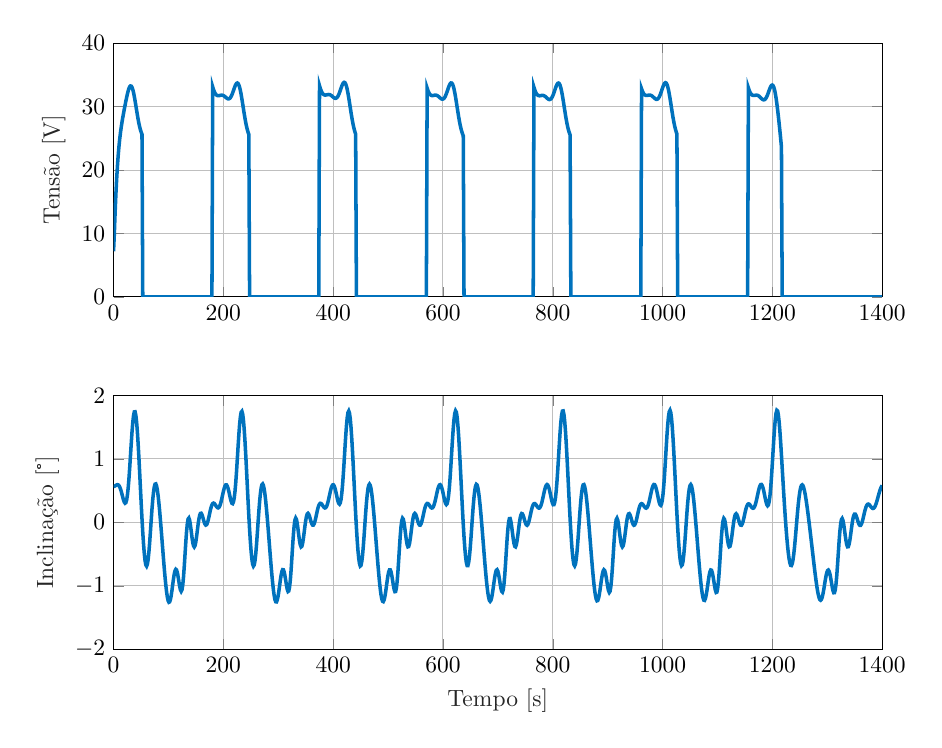
\begin{tikzpicture}[scale=0.85]

\begin{axis}[%
width=4.521in,
height=1.493in,
at={(0.758in,0.481in)},
scale only axis,
xmin=0,
xmax=1400,
xlabel style={font=\color{white!15!black}},
xlabel={Tempo [s]},
ymin=-2,
ymax=2,
ylabel style={font=\color{white!15!black}},
ylabel={Inclinação [\textdegree]},
axis background/.style={fill=white},
xmajorgrids,
ymajorgrids,
/pgf/number format/.cd,
        use comma,
        1000 sep={}
]
\addplot [color=mycolor1, line width=1.5pt, forget plot]
  table[row sep=crcr]{%
0	0.565429521954314\\
1.4	0.568330501953841\\
2.8	0.575284061576456\\
4.2	0.58351328911261\\
5.6	0.5906263573506\\
7	0.594019220015061\\
8.4	0.59116420098715\\
9.8	0.579952760623568\\
11.2	0.559058029519491\\
12.6	0.528267871235949\\
14	0.488740727156905\\
15.4	0.443148268943533\\
16.8	0.395682652274806\\
18.2	0.351914974301003\\
19.6	0.318492831210631\\
21	0.302661920574742\\
22.4	0.311597960742363\\
23.8	0.351552022909688\\
25.2	0.426853896100239\\
26.6	0.538884787845947\\
28	0.685207226239489\\
29.4	0.85909307798451\\
30.8	1.0496775268888\\
32.2	1.24285868371598\\
33.6	1.42287136841354\\
35	1.57425357480786\\
36.4	1.68378705919353\\
37.8	1.74199735990121\\
39.2	1.74394372012147\\
40.6	1.68924790048066\\
42	1.58150925803412\\
43.4	1.42736473448216\\
44.8	1.23546153608125\\
46.2	1.01554507090338\\
47.6	0.777768788629881\\
49	0.532242221246455\\
50.4	0.288768064454126\\
51.8	0.0566831017396174\\
53.2	-0.155406648213518\\
54.6	-0.340071264382529\\
56	-0.491016958815055\\
57.4	-0.602614277384731\\
58.8	-0.669975090082622\\
60.2	-0.689589804114836\\
61.6	-0.660154546226488\\
63	-0.583404730275611\\
64.4	-0.464704713819859\\
65.8	-0.313136832381185\\
67.2	-0.140921709538329\\
68.6	0.037818288718801\\
70	0.208727385652795\\
71.4	0.358937851145406\\
72.8	0.478447200990529\\
74.2	0.560878560802163\\
75.6	0.603556285882325\\
77	0.607019814109708\\
78.4	0.574207380339703\\
79.8	0.509552437820267\\
81.2	0.418177913925928\\
82.6	0.305290318774522\\
84	0.175801609362607\\
85.4	0.0341576134597039\\
86.8	-0.115671653909676\\
88.2	-0.270089660618774\\
89.6	-0.425704843582692\\
91	-0.579135642827138\\
92.4	-0.726825067594949\\
93.8	-0.864901060598177\\
95.2	-0.989122467527096\\
96.6	-1.09495402755556\\
98	-1.1778118345877\\
99.4	-1.23350568616952\\
100.8	-1.25886953204765\\
102.2	-1.25251369897268\\
103.6	-1.21556153299213\\
105	-1.15217232343524\\
106.4	-1.06963656337817\\
107.8	-0.977888625392201\\
109.2	-0.888417864765432\\
110.6	-0.812731927151651\\
112	-0.760664951637677\\
113.4	-0.738865283675001\\
114.8	-0.74972721980424\\
116.2	-0.790893495183529\\
117.6	-0.855325219225926\\
119	-0.931874392877467\\
120.4	-1.00631377319084\\
121.8	-1.06283957059116\\
123.2	-1.0860891087143\\
124.6	-1.06363006441991\\
126	-0.988644514086366\\
127.4	-0.86220928840567\\
128.8	-0.694344778258047\\
130.2	-0.50310579106326\\
131.6	-0.311540830206896\\
133	-0.143173638595859\\
134.4	-0.0173151037169223\\
135.8	0.0544193604173837\\
137.2	0.0695702133835\\
138.6	0.0342698389883894\\
140	-0.0387414532390502\\
141.4	-0.132743594605915\\
142.8	-0.229712644442806\\
144.2	-0.312741952540861\\
145.6	-0.368112813860426\\
147	-0.386959690004556\\
148.4	-0.366390641196107\\
149.8	-0.3098265560309\\
151.2	-0.22633574110929\\
152.6	-0.128926365112748\\
154	-0.032068855958102\\
155.4	0.0509974998794627\\
156.8	0.110527196033865\\
158.2	0.141610754333105\\
159.6	0.144427086610488\\
161	0.123555026797073\\
162.4	0.0866797580130641\\
163.8	0.0430547479105676\\
165.2	0.00199811581405822\\
166.6	-0.0284050540092729\\
168	-0.042300206336301\\
169.4	-0.0367004085754433\\
170.8	-0.0117137683024583\\
172.2	0.0296686772103376\\
173.6	0.0822053180349226\\
175	0.139361409600952\\
176.4	0.194420708255148\\
177.8	0.241540623634098\\
179.2	0.276559008727572\\
180.6	0.297437218352708\\
182	0.304290325117829\\
183.4	0.299062954727097\\
184.8	0.285068106764222\\
186.2	0.266516456081989\\
187.6	0.248028913118178\\
189	0.234143823011809\\
190.4	0.228839701882012\\
191.8	0.235096742100123\\
193.2	0.254529239073426\\
194.6	0.287131485907904\\
196	0.33118426603096\\
197.4	0.383360935859669\\
198.8	0.439048003487369\\
200.2	0.492858261782675\\
201.6	0.539274804918943\\
203	0.573334957986636\\
204.4	0.591255190600489\\
205.8	0.590914574329389\\
207.2	0.572148832712754\\
208.6	0.536846514999702\\
210	0.488869630484447\\
211.4	0.433834340391891\\
212.8	0.378781554849457\\
214.2	0.331747971369083\\
215.6	0.301225379786452\\
217	0.295482379944345\\
218.4	0.321730336025077\\
219.8	0.38515335995895\\
221.2	0.487890649705174\\
222.6	0.62814371419877\\
224	0.799647465998333\\
225.4	0.991747843565141\\
226.8	1.19023460472273\\
228.2	1.37889060638201\\
229.6	1.54149766588447\\
231	1.66387909018548\\
232.4	1.73553900642432\\
233.8	1.7505910950895\\
235.2	1.70789152743649\\
236.6	1.61050525290217\\
238	1.4647648861687\\
239.4	1.27920414842122\\
240.8	1.06358773607228\\
242.2	0.828161739718634\\
243.6	0.583153068158698\\
245	0.338475159616793\\
246.4	0.103556728705199\\
247.8	-0.112899357497125\\
249.2	-0.303379097069054\\
250.6	-0.46156357933842\\
252	-0.581787798365169\\
253.4	-0.659013072251953\\
254.8	-0.689400321909159\\
256.2	-0.671099786148547\\
257.6	-0.605094345565151\\
259	-0.495860843864129\\
260.4	-0.351590462998419\\
261.8	-0.183773800461407\\
263.2	-0.00611604292999509\\
264.6	0.167042566653315\\
266	0.322452938473141\\
267.4	0.449429075652043\\
268.8	0.540757952980848\\
270.2	0.592930566371713\\
271.6	0.605776169132957\\
273	0.581711332165182\\
274.4	0.524848178788958\\
275.8	0.440161908668586\\
277.2	0.332838321139694\\
278.6	0.207844803234933\\
280	0.069713352292902\\
281.4	-0.0775046497851307\\
282.8	-0.230160967653904\\
284.2	-0.384856952163774\\
285.6	-0.538254487154676\\
287	-0.686887507091332\\
288.4	-0.827009373842641\\
289.8	-0.954514224991991\\
291.2	-1.06497431623405\\
292.6	-1.1538354547949\\
294	-1.21680187522541\\
295.4	-1.25041297797183\\
296.8	-1.2527633397035\\
298.2	-1.22424960658262\\
299.6	-1.16816263776607\\
301	-1.0909126594283\\
302.4	-1.00171171930732\\
303.8	-0.91165273813057\\
305.2	-0.832290033884554\\
306.6	-0.773978609422495\\
308	-0.744300674994204\\
309.4	-0.746867552760524\\
310.8	-0.780661859904536\\
312.2	-0.839948398543891\\
313.6	-0.914700096635344\\
315	-0.991484942856555\\
316.4	-1.05481527752834\\
317.8	-1.08900493142342\\
319.2	-1.08053197111463\\
320.6	-1.02071215352698\\
322	-0.908177651801731\\
323.4	-0.750374145424935\\
324.8	-0.563272679017744\\
326.2	-0.368917880332036\\
327.6	-0.19122104437786\\
329	-0.0511645968558451\\
330.4	0.0371523412306256\\
331.8	0.0685985774369527\\
333.2	0.0469897450835835\\
334.6	-0.016568448524615\\
336	-0.106200890771016\\
337.4	-0.203975252093023\\
338.8	-0.292419261560544\\
340.2	-0.3567025665936\\
341.6	-0.386431597825917\\
343	-0.376947984006321\\
344.4	-0.32991462458229\\
345.8	-0.252945675605497\\
347.2	-0.158174255341577\\
348.6	-0.05993925985126\\
350	0.0279187153014284\\
351.4	0.0945046666322172\\
352.8	0.133502522107119\\
354.2	0.143728010859536\\
355.6	0.128670790018832\\
357	0.0953271246742561\\
358.4	0.0526916899971611\\
359.8	0.0102169040430251\\
361.2	-0.0235592386248887\\
362.6	-0.0421044458515709\\
364	-0.0416351158289382\\
365.4	-0.0214581275560964\\
366.8	0.0161264806571899\\
368.2	0.0663585083726781\\
369.6	0.122911193857257\\
371	0.17899031622049\\
372.4	0.228431179284462\\
373.8	0.266589077259047\\
375.2	0.290882427166721\\
376.6	0.300931495449687\\
378	0.298301502836894\\
379.4	0.286048946890224\\
380.8	0.268251057260356\\
382.2	0.249516380295531\\
383.6	0.234483036984997\\
385	0.227327130142228\\
386.4	0.231304354674407\\
387.8	0.248355837278588\\
389.2	0.278820068273967\\
390.6	0.321299293004568\\
392	0.372723427677225\\
393.4	0.428633062530823\\
394.8	0.483667224869662\\
396.2	0.532200262598254\\
397.6	0.56903895138137\\
399	0.590077984931324\\
400.4	0.592824430974051\\
401.8	0.576734638894401\\
403.2	0.54334787976958\\
404.6	0.496235201233875\\
406	0.440799211016642\\
407.4	0.383957823205089\\
408.8	0.333726891046476\\
410.2	0.298692912488105\\
411.6	0.287350206966643\\
413	0.307280057592997\\
414.4	0.364182471304966\\
415.8	0.460836792881258\\
417.2	0.596153220433922\\
418.6	0.76455197232679\\
420	0.95592480489407\\
421.4	1.15635480163971\\
422.8	1.34959080247057\\
424.2	1.51904486131432\\
425.6	1.64990006775698\\
427	1.73087012328385\\
428.4	1.75526667510701\\
429.8	1.72125101539716\\
431.2	1.63137414780584\\
432.6	1.49165828961391\\
434	1.31051125050143\\
435.4	1.09771268303025\\
436.8	0.863613409354614\\
438.2	0.618588820016913\\
439.6	0.372710511313324\\
441	0.13555500638797\\
442.4	-0.0840364267901897\\
443.8	-0.278441955737932\\
445.2	-0.441293825444085\\
446.6	-0.566891566625682\\
448	-0.650110309963535\\
449.4	-0.686936051993582\\
450.8	-0.675231531988233\\
452.2	-0.615580854399959\\
453.6	-0.511985540859603\\
455	-0.372152915449985\\
456.4	-0.207169605297542\\
457.8	-0.0305011626584035\\
459.2	0.143534568767061\\
460.6	0.301490823099082\\
462	0.432311474006734\\
463.4	0.528321382123947\\
464.8	0.585544183722464\\
466.2	0.603405981267087\\
467.6	0.584024050392115\\
469	0.531324543159713\\
470.4	0.450197047805156\\
471.8	0.345817105597872\\
473.2	0.223189114920447\\
474.6	0.0869039749853657\\
476	-0.0589261487337707\\
477.4	-0.210604494490656\\
478.8	-0.364704981143218\\
480.2	-0.517887462408059\\
481.6	-0.66670946550235\\
483	-0.807469595894142\\
484.4	-0.93612012337695\\
485.8	-1.04829003324284\\
487.2	-1.13946042536269\\
488.6	-1.20532486817904\\
490	-1.2423408417138\\
491.4	-1.24843034177545\\
492.8	-1.22372208822025\\
494.2	-1.17116205223851\\
495.6	-1.09678371047357\\
497	-1.00945726355227\\
498.4	-0.920042392318799\\
499.8	-0.840029093135209\\
501.2	-0.779906023853591\\
502.6	-0.747577250941711\\
504	-0.747120842458709\\
505.4	-0.778068073265\\
506.8	-0.835245809785375\\
508.2	-0.909135802855512\\
509.6	-0.9866957761211\\
511	-1.05263878325715\\
512.4	-1.0912166012499\\
513.8	-1.08851966150177\\
515.2	-1.03513125939098\\
516.6	-0.928671642982443\\
518	-0.775469542078349\\
519.4	-0.590535239920269\\
520.8	-0.395376691568409\\
522.2	-0.213958960619582\\
523.6	-0.0678983130105605\\
525	0.0276727334890028\\
526.4	0.0664575382974802\\
527.8	0.0512233784164742\\
529.2	-0.00769405018696023\\
530.6	-0.0948497302708784\\
532	-0.192410426143925\\
533.4	-0.28271281191242\\
534.8	-0.350493909022015\\
536.2	-0.384739474222325\\
537.6	-0.380052438628037\\
539	-0.337336648251718\\
540.4	-0.263548338700333\\
541.8	-0.17038437449301\\
543.2	-0.0720510238957114\\
544.6	0.0174278117705452\\
546	0.0867212759197755\\
547.4	0.128940663604655\\
548.8	0.142320608086359\\
550.2	0.12986583550516\\
551.6	0.0982460293624593\\
553	0.0563075186141391\\
554.4	0.0135215171562104\\
555.8	-0.0214170841213515\\
557.2	-0.0417190421455493\\
558.6	-0.043286752226112\\
560	-0.0251022539606417\\
561.4	0.0108234788633127\\
562.8	0.0599422609953466\\
564.2	0.116034134524113\\
565.6	0.172298098534555\\
567	0.222462591419465\\
568.4	0.261707211832008\\
569.8	0.287243942133434\\
571.2	0.298502632350296\\
572.6	0.296914677915417\\
574	0.285451490332556\\
575.4	0.268131422781662\\
576.8	0.249528626358146\\
578.2	0.2342757119324\\
579.6	0.22657733014086\\
581	0.229755737634793\\
582.4	0.245857039766631\\
583.8	0.275357763404111\\
585.2	0.317018768454839\\
586.6	0.367929822589482\\
588	0.423768729689229\\
589.4	0.479264843569547\\
590.8	0.528816273241693\\
592.2	0.567176063585962\\
593.6	0.590107525630651\\
595	0.594918572559055\\
596.4	0.580815624927556\\
597.8	0.549057648871581\\
599.2	0.502925906653064\\
600.6	0.447544188274594\\
602	0.389583847154409\\
603.4	0.336871410921818\\
604.8	0.29789284867981\\
606.2	0.281169706461153\\
607.6	0.294480966848021\\
609	0.343931362553421\\
610.4	0.43292621831747\\
611.8	0.561195995711277\\
613.2	0.724093434449575\\
614.6	0.9124192163064\\
616	1.11297552375446\\
617.4	1.30988715500766\\
618.8	1.48650702880506\\
620.2	1.62752556761612\\
621.6	1.72082525131945\\
623	1.75870385446893\\
624.4	1.73829381930786\\
625.8	1.66123737263029\\
627.2	1.53284591293239\\
628.6	1.36103355007805\\
630	1.15527877277077\\
631.4	0.925777186937396\\
632.8	0.682846845780092\\
634.2	0.436565345928448\\
635.6	0.19656585960511\\
637	-0.028102972960798\\
638.4	-0.229444136361636\\
639.8	-0.40080950182261\\
641.2	-0.536384537759663\\
642.6	-0.63089729606097\\
644	-0.680020176382028\\
645.4	-0.681082350823237\\
646.8	-0.633906638198324\\
648.2	-0.541562030265498\\
649.6	-0.410776597487283\\
651	-0.251783010528387\\
652.4	-0.077492604574644\\
653.8	0.0979099339727077\\
655.2	0.260663872507722\\
656.6	0.399029523048891\\
658	0.504430512361348\\
659.4	0.571946417813873\\
660.8	0.600164416067276\\
662.2	0.590559180574672\\
663.6	0.546639942872856\\
665	0.473085743751644\\
666.4	0.375020473201382\\
667.8	0.257499036129229\\
669.2	0.125211923123274\\
670.6	-0.017622916739003\\
672	-0.167227646572743\\
673.4	-0.320139381873973\\
674.8	-0.473034925063683\\
676.2	-0.622542559530578\\
677.6	-0.765075626874199\\
679	-0.896723947211615\\
680.4	-1.01324270298765\\
681.8	-1.11018032114216\\
683.2	-1.18318109585151\\
684.6	-1.22847757937476\\
686	-1.24354661330084\\
687.4	-1.22784237511145\\
688.8	-1.18345307480021\\
690.2	-1.11548168584504\\
691.6	-1.0319582838765\\
693	-0.943173443029661\\
694.4	-0.860467818353116\\
695.8	-0.794673018118209\\
697.2	-0.754504991930098\\
698.6	-0.745215895604272\\
700	-0.76771821240886\\
701.4	-0.818260594661521\\
702.8	-0.888629280773382\\
704.2	-0.966817268253803\\
705.6	-1.0381418722985\\
707	-1.08684908318852\\
708.4	-1.09824303568216\\
709.8	-1.06125110747431\\
711.2	-0.971065146958698\\
712.6	-0.831178732336205\\
714	-0.653975982139545\\
715.4	-0.459246703653351\\
716.8	-0.270660088997983\\
718.2	-0.111061131378663\\
719.6	0.00201680635938545\\
721	0.059343749172558\\
722.4	0.0608830083110905\\
723.8	0.0147728048361979\\
725.2	-0.0649068633116942\\
726.6	-0.160827737213262\\
728	-0.255046467198438\\
729.4	-0.331342240582169\\
730.8	-0.377188060369974\\
732.2	-0.385284671577419\\
733.6	-0.35448696322013\\
735	-0.289876525648088\\
736.4	-0.201793714575078\\
737.8	-0.103872892841468\\
739.2	-0.0104431117041452\\
740.6	0.0661021702003135\\
742	0.117341496197051\\
743.4	0.139859603061089\\
744.8	0.135206865263692\\
746.2	0.109001348756508\\
747.6	0.0695302186132302\\
749	0.0261948085213907\\
750.4	-0.011951988665728\\
751.8	-0.0374289970835738\\
753.2	-0.0452276451352402\\
754.6	-0.0333321477582113\\
756	-0.0028121629619048\\
757.4	0.0425301801601768\\
758.8	0.096916530590558\\
760.2	0.153628834234976\\
761.6	0.206134559135599\\
763	0.249086806127748\\
764.4	0.27902423012658\\
765.8	0.294683387824319\\
767.2	0.29690897260528\\
768.6	0.288247044150578\\
770	0.272440025246579\\
771.4	0.253935201881093\\
772.8	0.237389651661159\\
774.2	0.227180496470577\\
775.6	0.226940107523396\\
777	0.239141515453448\\
778.4	0.264769926854188\\
779.8	0.303125653712783\\
781.2	0.351804369293328\\
782.6	0.406886495476988\\
784	0.463337715175281\\
785.4	0.515583039362574\\
786.8	0.558179387188971\\
788.2	0.586489488030176\\
789.6	0.597261573478076\\
791	0.589044198605297\\
792.4	0.562404032686592\\
793.8	0.519952494600195\\
795.2	0.466212215490369\\
796.6	0.407360213589515\\
798	0.350872581847533\\
799.4	0.305072763571489\\
800.8	0.27856320623459\\
802.2	0.279510911754358\\
803.6	0.314772900164959\\
805	0.388895173689714\\
806.4	0.503095385634983\\
807.8	0.654425232357875\\
809.2	0.835365270444725\\
810.6	1.03408629710867\\
812	1.23548915405188\\
813.4	1.42292702978329\\
814.8	1.58029459148311\\
816.2	1.69403555011203\\
817.6	1.75464173733812\\
819	1.75738401972349\\
820.4	1.70224959983771\\
821.8	1.59326209020225\\
823.2	1.43746471025027\\
824.6	1.24384410268994\\
826	1.02239638968141\\
827.4	0.78343497331398\\
828.8	0.537147610465581\\
830.2	0.293346195686254\\
831.6	0.0613193913871264\\
833	-0.150444865185534\\
834.4	-0.33468297146795\\
835.8	-0.485253020282636\\
837.2	-0.596662269130802\\
838.6	-0.664157260785265\\
840	-0.684346555226713\\
841.4	-0.656007765908025\\
842.8	-0.580898753489878\\
844.2	-0.464329200923388\\
845.6	-0.31524377757363\\
847	-0.145654751419871\\
848.4	0.0305637430013251\\
849.8	0.199301618467035\\
851.2	0.347892335840711\\
852.6	0.466460712241013\\
854	0.548673395740317\\
855.4	0.591823611381673\\
856.8	0.596366799344938\\
858.2	0.565130296923044\\
859.6	0.502432814095329\\
861	0.413294859325917\\
862.4	0.302841219209415\\
863.8	0.175924463869453\\
865.2	0.0369501291840802\\
866.6	-0.110139315111868\\
868	-0.261770265445759\\
869.4	-0.414578520218149\\
870.8	-0.565223676804444\\
872.2	-0.710212709343979\\
873.6	-0.845767934576708\\
875	-0.967777442552901\\
876.4	-1.07186891540505\\
877.8	-1.15364531631668\\
879.2	-1.20910629992738\\
880.6	-1.23524593905984\\
882	-1.23076368666886\\
883.4	-1.1967596823607\\
884.8	-1.13722939568091\\
886.2	-1.0591578483067\\
887.6	-0.972067539688328\\
889	-0.886998925852076\\
890.4	-0.815061940789608\\
891.8	-0.765827482724972\\
893.2	-0.745870658932271\\
894.6	-0.757717252882149\\
896	-0.799319896135345\\
897.4	-0.864069574798178\\
898.8	-0.941288820524088\\
900.2	-1.01716998450475\\
901.6	-1.0761806061331\\
903	-1.1029880783377\\
904.4	-1.08488076478906\\
905.8	-1.01444115837494\\
907.2	-0.891905730578933\\
908.6	-0.726393719187187\\
910	-0.535241850523628\\
911.4	-0.341187788051733\\
912.8	-0.167962271021863\\
914.2	-0.0355493468043163\\
915.6	0.0434822072585952\\
917	0.0656746717912188\\
918.4	0.0363141919909041\\
919.8	-0.0324420212323702\\
921.2	-0.124165601919788\\
922.6	-0.220856242365178\\
924	-0.305404837513412\\
925.4	-0.363707197281131\\
926.8	-0.386373872093599\\
928.2	-0.369907451238002\\
929.6	-0.317119375382942\\
931	-0.236558143254008\\
932.4	-0.140890628078858\\
933.8	-0.0444799116864481\\
935.2	0.0393071638003675\\
936.6	0.100416819623831\\
938	0.133539349687479\\
939.4	0.138454363102494\\
940.8	0.119413798654755\\
942.2	0.0838867296015326\\
943.6	0.0410284205715224\\
945	0.000161941824751445\\
946.4	-0.0305457186544446\\
947.8	-0.0451110234126847\\
949.2	-0.0403999429292747\\
950.6	-0.0163807722987167\\
952	0.0240682963658033\\
953.4	0.0757797345370712\\
954.8	0.132251818418638\\
956.2	0.186767447099545\\
957.6	0.233463657148003\\
959	0.268155775372409\\
960.4	0.288792266564601\\
961.8	0.29551369007278\\
963.2	0.290331980034688\\
964.6	0.276631530018778\\
966	0.258678911395864\\
967.4	0.241128273708838\\
968.8	0.228523648291511\\
970.2	0.224818280666408\\
971.6	0.232934172987521\\
973	0.254394627774425\\
974.4	0.289073359945322\\
975.8	0.335108177785744\\
977.2	0.389018347522947\\
978.6	0.446039499183735\\
980	0.500651908611376\\
981.4	0.547237607076061\\
982.8	0.580772722159093\\
984.2	0.59745467072791\\
985.6	0.595182022282273\\
987	0.573840965216873\\
988.4	0.535392793725644\\
989.8	0.483787778092415\\
991.2	0.424743395213413\\
992.6	0.365417963092271\\
994	0.313989920316094\\
995.4	0.279128601445077\\
996.8	0.26932689338448\\
998.2	0.292072173463261\\
999.6	0.352868971527012\\
1001	0.454196171472714\\
1002.4	0.594569461114699\\
1003.8	0.767952957512832\\
1005.2	0.96377579292726\\
1006.6	1.16772118603\\
1008	1.36326715126175\\
1009.4	1.53372713459837\\
1010.8	1.66436383739033\\
1012.2	1.74411636396208\\
1013.6	1.76660864593698\\
1015	1.73033483263418\\
1016.4	1.63814341677864\\
1017.8	1.49628361272842\\
1019.2	1.31330723000182\\
1020.6	1.09906059769451\\
1022	0.863900789936187\\
1023.4	0.618170707626732\\
1024.8	0.371892648962566\\
1026.2	0.134596707935644\\
1027.6	-0.0848371009185257\\
1029	-0.278680750203403\\
1030.4	-0.440547287782728\\
1031.8	-0.564802784004346\\
1033.2	-0.646424494276927\\
1034.6	-0.681542674782398\\
1036	-0.668205172999863\\
1037.4	-0.60720857995853\\
1038.8	-0.502767140535284\\
1040.2	-0.362763856640974\\
1041.6	-0.198385698512118\\
1043	-0.0230962871305862\\
1044.4	0.14889584239589\\
1045.8	0.304340571181534\\
1047.2	0.43242658823543\\
1048.6	0.525726077299265\\
1050	0.580473751291588\\
1051.4	0.596247422076398\\
1052.8	0.575251095927511\\
1054.2	0.521440904225202\\
1055.6	0.439695566702228\\
1057	0.335156639517553\\
1058.4	0.212786956564325\\
1059.8	0.0771396441032789\\
1061.2	-0.067700361198298\\
1062.6	-0.218050507396721\\
1064	-0.370487165788665\\
1065.4	-0.521665477608578\\
1066.8	-0.668138826199478\\
1068.2	-0.806213001144408\\
1069.6	-0.931872196656511\\
1071	-1.04081701644304\\
1072.4	-1.12865399230078\\
1073.8	-1.19126524628884\\
1075.2	-1.22535908641346\\
1076.6	-1.22915413537047\\
1078	-1.20308624301629\\
1079.4	-1.15036700752651\\
1080.8	-1.07719481464971\\
1082.2	-0.99245362824725\\
1083.6	-0.906841591211996\\
1085	-0.831525276357875\\
1086.4	-0.776557845437315\\
1087.8	-0.749367744783808\\
1089.2	-0.753590130191011\\
1090.6	-0.788400952336316\\
1092	-0.848387157638379\\
1093.4	-0.923909052460608\\
1094.8	-1.00190986321869\\
1096.2	-1.06718081784435\\
1097.6	-1.10413535029569\\
1099	-1.09910517004445\\
1100.4	-1.04298813048086\\
1101.8	-0.933771174809596\\
1103.2	-0.778156679181676\\
1104.6	-0.591469061354057\\
1106	-0.395401888695851\\
1107.4	-0.213933542660479\\
1108.8	-0.0685236126547702\\
1110.2	0.0259735763756262\\
1111.6	0.063587068944463\\
1113	0.0473855220558263\\
1114.4	-0.012068525383031\\
1115.8	-0.0992020070656516\\
1117.2	-0.196157211213854\\
1118.6	-0.285344136239593\\
1120	-0.351659424886846\\
1121.4	-0.384316468038358\\
1122.8	-0.378184537250184\\
1124.2	-0.334429948645231\\
1125.6	-0.260216242860707\\
1127	-0.167344911732065\\
1128.4	-0.0699964762939876\\
1129.8	0.0179578499825381\\
1131.2	0.0854324714544141\\
1132.6	0.125823212641839\\
1134	0.137633549236107\\
1135.4	0.12407882174116\\
1136.8	0.091956860539462\\
1138.2	0.0501520150711119\\
1139.6	0.00808706575038029\\
1141	-0.0256675386560951\\
1142.4	-0.0445075388125742\\
1143.8	-0.0445597243812525\\
1145.2	-0.0250422160299412\\
1146.6	0.0118193700144577\\
1148	0.0613175766844315\\
1149.4	0.117156048821273\\
1150.8	0.17255413279451\\
1152.2	0.221353639776113\\
1153.6	0.258920463030166\\
1155	0.282695129853129\\
1156.4	0.292343666059201\\
1157.8	0.289519383262215\\
1159.2	0.27738004565135\\
1160.6	0.26007098029878\\
1162	0.242223988634758\\
1163.4	0.22845669293545\\
1164.8	0.222886232908963\\
1166.2	0.228678598537277\\
1167.6	0.247663665729906\\
1169	0.280057297823357\\
1170.4	0.324338388460419\\
1171.8	0.377323076497802\\
1173.2	0.43445643103666\\
1174.6	0.490305816478392\\
1176	0.539199107136286\\
1177.4	0.57591842923585\\
1178.8	0.596348209123794\\
1180.2	0.597989703848566\\
1181.6	0.580287701856409\\
1183	0.544756023378282\\
1184.4	0.494922458793906\\
1185.8	0.436130698753445\\
1187.2	0.375233830655069\\
1188.6	0.320195508614553\\
1190	0.279590425209245\\
1191.4	0.261977313033958\\
1192.8	0.275117917214572\\
1194.2	0.325044500197842\\
1195.6	0.415039958325003\\
1197	0.544678726648489\\
1198.4	0.709154994933693\\
1199.8	0.899153486231208\\
1201.2	1.10145523404491\\
1202.6	1.30030565199989\\
1204	1.47934817568669\\
1205.4	1.62373413723355\\
1206.8	1.72195011013528\\
1208.2	1.76699434524995\\
1209.6	1.7567410092198\\
1211	1.6935599761535\\
1212.4	1.58342175299688\\
1213.8	1.43477134218104\\
1215.2	1.25741509027764\\
1216.6	1.06157467892941\\
1218	0.856967798106425\\
1219.4	0.651538679136281\\
1220.8	0.450752975320094\\
1222.2	0.258329298867554\\
1223.6	0.0771160871684836\\
1225	-0.090497485578495\\
1226.4	-0.242260365079539\\
1227.8	-0.375839792234405\\
1229.2	-0.488710338204497\\
1230.6	-0.578159649229569\\
1232	-0.641418081930664\\
1233.4	-0.675913306254711\\
1234.8	-0.679636271846077\\
1236.2	-0.651581075549903\\
1237.6	-0.592191853547393\\
1239	-0.503723721829899\\
1240.4	-0.39041487655321\\
1241.8	-0.258385419243542\\
1243.2	-0.115229500659083\\
1244.6	0.0306588173848919\\
1246	0.170912450072712\\
1247.4	0.298012882091523\\
1248.8	0.405950914639705\\
1250.2	0.490619183160251\\
1251.6	0.549902657296768\\
1253	0.583504405279217\\
1254.4	0.59259055079163\\
1255.8	0.579352691790133\\
1257.2	0.546573485186844\\
1258.6	0.497253896968375\\
1260	0.434330973893839\\
1261.4	0.360490945437548\\
1262.8	0.27806713251985\\
1264.2	0.189005043291739\\
1265.6	0.0948759505955025\\
1267	-0.00307735241035847\\
1268.4	-0.103875082048169\\
1269.8	-0.20672381927941\\
1271.2	-0.310933970052563\\
1272.6	-0.415834352340815\\
1274	-0.520685795893038\\
1275.4	-0.624595668057729\\
1276.8	-0.726436454822414\\
1278.2	-0.824773937143514\\
1279.6	-0.917814017633597\\
1281	-1.00338152748913\\
1282.4	-1.07894856184955\\
1283.8	-1.14173254022833\\
1285.2	-1.18888296350342\\
1286.6	-1.21776791817603\\
1288	-1.226354332593\\
1289.4	-1.21364944916788\\
1290.8	-1.1801386886603\\
1292.2	-1.12812621391163\\
1293.6	-1.06187245136666\\
1295	-0.987440310248373\\
1296.4	-0.912213184835582\\
1297.8	-0.844122682511408\\
1299.2	-0.790697981506242\\
1300.6	-0.758093346838086\\
1302	-0.750248169653434\\
1303.4	-0.768288974941666\\
1304.8	-0.810219153242227\\
1306.2	-0.870890944812416\\
1307.6	-0.942238141758852\\
1309	-1.01377073815949\\
1310.4	-1.07337653358106\\
1311.8	-1.10850399661968\\
1313.2	-1.10777144334533\\
1314.6	-1.0629246631667\\
1316	-0.970851434641378\\
1317.4	-0.835128934723302\\
1318.8	-0.666471847763322\\
1320.2	-0.481614293637858\\
1321.6	-0.300629136808516\\
1323	-0.14328712265764\\
1324.4	-0.0254647211485296\\
1325.8	0.0434217224176483\\
1327.2	0.0614219272249392\\
1328.6	0.0335473514781038\\
1330	-0.0297777928969677\\
1331.4	-0.114734631957056\\
1332.8	-0.206155393328249\\
1334.2	-0.289374558042638\\
1335.6	-0.351828605470484\\
1337	-0.384397391301892\\
1338.4	-0.382428253115301\\
1339.8	-0.346294648277168\\
1341.2	-0.281297633885444\\
1342.6	-0.196784805714574\\
1344	-0.104543461278734\\
1345.4	-0.0167538130019103\\
1346.8	0.0560501353496948\\
1348.2	0.106559921311214\\
1349.6	0.131517843430159\\
1351	0.131732087394336\\
1352.4	0.111433812078533\\
1353.8	0.0772338380182104\\
1355.2	0.0369346124223094\\
1356.6	-0.00161315303236328\\
1358	-0.0314969810381228\\
1359.4	-0.0475134061983532\\
1360.8	-0.0466860826783759\\
1362.2	-0.0284979925377819\\
1363.6	0.00518874960386559\\
1365	0.0505260327384412\\
1366.4	0.102338943858341\\
1367.8	0.15494902568524\\
1369.2	0.20301978751516\\
1370.6	0.242277696425238\\
1372	0.269996542721902\\
1373.4	0.285194599388527\\
1374.8	0.28855944099957\\
1376.2	0.282163628480553\\
1377.6	0.26905554585658\\
1379	0.252805734880534\\
1380.4	0.237070126556033\\
1381.8	0.225208928453328\\
1383.2	0.219981552299255\\
1384.6	0.223326879201703\\
1386	0.236233255298537\\
1387.4	0.258700568194944\\
1388.8	0.289794035243675\\
1390.2	0.327783717079919\\
1391.6	0.370355158850248\\
1393	0.414866933880242\\
1394.4	0.458623382163673\\
1395.8	0.499128447249884\\
1397.2	0.534290628968277\\
1398.6	0.56255891444678\\
1400	0.58298250433618\\
};
\end{axis}

\begin{axis}[%
width=4.521in,
height=1.493in,
at={(0.758in,2.554in)},
scale only axis,
xmin=0,
xmax=1400,
ymin=0,
ymax=40,
ylabel style={font=\color{white!15!black}},
ylabel={Tensão [V]},
axis background/.style={fill=white},
xmajorgrids,
ymajorgrids,
/pgf/number format/.cd,
        use comma,
        1000 sep={}
]
\addplot [color=mycolor1, line width=1.5pt, forget plot]
  table[row sep=crcr]{%
0	7.2\\
1.4	9.91311980637246\\
2.8	13.2327909160965\\
4.2	16.0768035134712\\
5.6	18.490790371854\\
7	20.5246494214964\\
8.4	22.229971906583\\
9.8	23.6581790761685\\
11.2	24.8590929521143\\
12.6	25.8797298521196\\
14	26.7631836690189\\
15.4	27.5475380949128\\
16.8	28.2648034712387\\
18.2	28.9399151917777\\
19.6	29.5898630735289\\
21	30.2230520516328\\
22.4	30.8390264643909\\
23.8	31.4287167659708\\
25.2	31.9753724019451\\
26.6	32.45630508315\\
28	32.8454635823215\\
29.4	33.1166936005135\\
30.8	33.2473350934285\\
32.2	33.2216383376112\\
33.6	33.033415168449\\
35	32.6874344785665\\
36.4	32.1993128756631\\
37.8	31.5939683747666\\
39.2	30.9029894681286\\
40.6	30.1614343368088\\
42	29.4045827973662\\
43.4	28.6650457447382\\
44.8	27.9704580691038\\
46.2	27.3418073081559\\
47.6	26.7923254319807\\
49	26.3268107522441\\
50.4	25.9412450242212\\
51.8	25.6226092513272\\
53.2	0\\
54.6	0\\
56	0\\
57.4	0\\
58.8	0\\
60.2	0\\
61.6	0\\
63	0\\
64.4	0\\
65.8	0\\
67.2	0\\
68.6	0\\
70	0\\
71.4	0\\
72.8	0\\
74.2	0\\
75.6	0\\
77	0\\
78.4	0\\
79.8	0\\
81.2	0\\
82.6	0\\
84	0\\
85.4	0\\
86.8	0\\
88.2	0\\
89.6	0\\
91	0\\
92.4	0\\
93.8	0\\
95.2	0\\
96.6	0\\
98	0\\
99.4	0\\
100.8	0\\
102.2	0\\
103.6	0\\
105	0\\
106.4	0\\
107.8	0\\
109.2	0\\
110.6	0\\
112	0\\
113.4	0\\
114.8	0\\
116.2	0\\
117.6	0\\
119	0\\
120.4	0\\
121.8	0\\
123.2	0\\
124.6	0\\
126	0\\
127.4	0\\
128.8	0\\
130.2	0\\
131.6	0\\
133	0\\
134.4	0\\
135.8	0\\
137.2	0\\
138.6	0\\
140	0\\
141.4	0\\
142.8	0\\
144.2	0\\
145.6	0\\
147	0\\
148.4	0\\
149.8	0\\
151.2	0\\
152.6	0\\
154	0\\
155.4	0\\
156.8	0\\
158.2	0\\
159.6	0\\
161	0\\
162.4	0\\
163.8	0\\
165.2	0\\
166.6	0\\
168	0\\
169.4	0\\
170.8	0\\
172.2	0\\
173.6	0\\
175	0\\
176.4	0\\
177.8	0\\
179.2	0\\
180.6	33.0898883501331\\
182	32.696625535963\\
183.4	32.3747270766886\\
184.8	32.1219877539991\\
186.2	31.9352803622082\\
187.6	31.809642015076\\
189	31.7377838160059\\
190.4	31.7100184007228\\
191.8	31.7145884603719\\
193.2	31.7383612322383\\
194.6	31.7678258298443\\
196	31.7902937737482\\
197.4	31.7951655709028\\
198.8	31.7750993728501\\
200.2	31.726913736709\\
201.6	31.6520826223596\\
203	31.5567352689707\\
204.4	31.4511450407181\\
205.8	31.3487621989983\\
207.2	31.2648989200744\\
208.6	31.2152008021042\\
210	31.2140378546931\\
211.4	31.2729288981832\\
212.8	31.3990905816136\\
214.2	31.5941894413475\\
215.6	31.853380857196\\
217	32.1647421030507\\
218.4	32.5092372376293\\
219.8	32.8613685509992\\
221.2	33.1906456787576\\
222.6	33.4639154333825\\
224	33.6484366396246\\
225.4	33.7153806516199\\
226.8	33.6432513730697\\
228.2	33.4206284104247\\
229.6	33.047704229166\\
231	32.5363138199327\\
232.4	31.9084761981814\\
233.8	31.1937714599602\\
235.2	30.4260662393806\\
236.6	29.640130706044\\
238	28.8685836558798\\
239.4	28.1394227782323\\
240.8	27.474214721884\\
242.2	26.8868826074655\\
243.6	26.3829602334809\\
245	25.9591642985586\\
246.4	25.6031853637018\\
247.8	0\\
249.2	0\\
250.6	0\\
252	0\\
253.4	0\\
254.8	0\\
256.2	0\\
257.6	0\\
259	0\\
260.4	0\\
261.8	0\\
263.2	0\\
264.6	0\\
266	0\\
267.4	0\\
268.8	0\\
270.2	0\\
271.6	0\\
273	0\\
274.4	0\\
275.8	0\\
277.2	0\\
278.6	0\\
280	0\\
281.4	0\\
282.8	0\\
284.2	0\\
285.6	0\\
287	0\\
288.4	0\\
289.8	0\\
291.2	0\\
292.6	0\\
294	0\\
295.4	0\\
296.8	0\\
298.2	0\\
299.6	0\\
301	0\\
302.4	0\\
303.8	0\\
305.2	0\\
306.6	0\\
308	0\\
309.4	0\\
310.8	0\\
312.2	0\\
313.6	0\\
315	0\\
316.4	0\\
317.8	0\\
319.2	0\\
320.6	0\\
322	0\\
323.4	0\\
324.8	0\\
326.2	0\\
327.6	0\\
329	0\\
330.4	0\\
331.8	0\\
333.2	0\\
334.6	0\\
336	0\\
337.4	0\\
338.8	0\\
340.2	0\\
341.6	0\\
343	0\\
344.4	0\\
345.8	0\\
347.2	0\\
348.6	0\\
350	0\\
351.4	0\\
352.8	0\\
354.2	0\\
355.6	0\\
357	0\\
358.4	0\\
359.8	0\\
361.2	0\\
362.6	0\\
364	0\\
365.4	0\\
366.8	0\\
368.2	0\\
369.6	0\\
371	0\\
372.4	0\\
373.8	0\\
375.2	33.2745129943574\\
376.6	32.8676901785413\\
378	32.5324312415245\\
379.4	32.2666369025012\\
380.8	32.0675307028104\\
382.2	31.9306342788169\\
383.6	31.8491762556053\\
385	31.8139280452164\\
386.4	31.8134530404979\\
387.8	31.8347386498073\\
389.2	31.8641537558875\\
390.6	31.8886379292327\\
392	31.8969894960485\\
393.4	31.8810887322589\\
394.8	31.8368828278032\\
396.2	31.7649797641237\\
397.6	31.6707491265973\\
399	31.5638991026343\\
400.4	31.4575731560911\\
401.8	31.3670689882827\\
403.2	31.3083144256744\\
404.6	31.2962380959832\\
406	31.3431553636178\\
407.4	31.457266105601\\
408.8	31.641345027439\\
410.2	31.8917071660028\\
411.6	32.197552447809\\
413	32.5408246081632\\
414.4	32.8967417022992\\
415.8	33.2351406527911\\
417.2	33.5227006593964\\
418.6	33.7259591200957\\
420	33.8148292728293\\
421.4	33.7661289421195\\
422.8	33.5665160004568\\
424.2	33.214267201072\\
425.6	32.7195473048798\\
427	32.1031361364862\\
428.4	31.3939030753177\\
429.8	30.6255343479588\\
431.2	29.8330734745436\\
432.6	29.0497429793408\\
434	28.3043374704684\\
435.4	27.6192876163606\\
436.8	27.0093528161792\\
438.2	26.4808047106352\\
439.6	26.0309478508769\\
441	25.647912886635\\
442.4	0\\
443.8	0\\
445.2	0\\
446.6	0\\
448	0\\
449.4	0\\
450.8	0\\
452.2	0\\
453.6	0\\
455	0\\
456.4	0\\
457.8	0\\
459.2	0\\
460.6	0\\
462	0\\
463.4	0\\
464.8	0\\
466.2	0\\
467.6	0\\
469	0\\
470.4	0\\
471.8	0\\
473.2	0\\
474.6	0\\
476	0\\
477.4	0\\
478.8	0\\
480.2	0\\
481.6	0\\
483	0\\
484.4	0\\
485.8	0\\
487.2	0\\
488.6	0\\
490	0\\
491.4	0\\
492.8	0\\
494.2	0\\
495.6	0\\
497	0\\
498.4	0\\
499.8	0\\
501.2	0\\
502.6	0\\
504	0\\
505.4	0\\
506.8	0\\
508.2	0\\
509.6	0\\
511	0\\
512.4	0\\
513.8	0\\
515.2	0\\
516.6	0\\
518	0\\
519.4	0\\
520.8	0\\
522.2	0\\
523.6	0\\
525	0\\
526.4	0\\
527.8	0\\
529.2	0\\
530.6	0\\
532	0\\
533.4	0\\
534.8	0\\
536.2	0\\
537.6	0\\
539	0\\
540.4	0\\
541.8	0\\
543.2	0\\
544.6	0\\
546	0\\
547.4	0\\
548.8	0\\
550.2	0\\
551.6	0\\
553	0\\
554.4	0\\
555.8	0\\
557.2	0\\
558.6	0\\
560	0\\
561.4	0\\
562.8	0\\
564.2	0\\
565.6	0\\
567	0\\
568.4	0\\
569.8	0\\
571.2	32.904595020109\\
572.6	32.5425635964837\\
574	32.2539373341897\\
575.4	32.0353201992633\\
576.8	31.8818078321231\\
578.2	31.7863495610993\\
579.6	31.7395375100914\\
581	31.7298081644743\\
582.4	31.7440266698941\\
583.8	31.768399515834\\
585.2	31.7896268247735\\
586.6	31.7961670397584\\
588	31.7794552489626\\
589.4	31.7349043813801\\
590.8	31.6625354521725\\
592.2	31.5671302042249\\
593.6	31.4578680516163\\
595	31.3474826875726\\
596.4	31.2510340362531\\
597.8	31.1844257326918\\
599.2	31.1628041176661\\
600.6	31.1989588864235\\
602	31.301821460472\\
603.4	31.4751393701169\\
604.8	31.7164040044952\\
606.2	32.016127876974\\
607.6	32.3575989636108\\
609	32.7172660388937\\
610.4	33.0659043400298\\
611.8	33.3706483689445\\
613.2	33.5978432513945\\
614.6	33.7164707060834\\
616	33.7017003497363\\
617.4	33.5379798638389\\
618.8	33.221082784198\\
620.2	32.7587082898554\\
621.6	32.1695300574795\\
623	31.4809196777306\\
624.4	30.7258129848411\\
625.8	29.9392770518696\\
627.2	29.155270218925\\
628.6	28.4039269798204\\
630	27.7095059894109\\
631.4	27.08897301845\\
632.8	26.5511043763533\\
634.2	26.0959632824797\\
635.6	25.7146562686147\\
637	25.3892186783877\\
638.4	0\\
639.8	0\\
641.2	0\\
642.6	0\\
644	0\\
645.4	0\\
646.8	0\\
648.2	0\\
649.6	0\\
651	0\\
652.4	0\\
653.8	0\\
655.2	0\\
656.6	0\\
658	0\\
659.4	0\\
660.8	0\\
662.2	0\\
663.6	0\\
665	0\\
666.4	0\\
667.8	0\\
669.2	0\\
670.6	0\\
672	0\\
673.4	0\\
674.8	0\\
676.2	0\\
677.6	0\\
679	0\\
680.4	0\\
681.8	0\\
683.2	0\\
684.6	0\\
686	0\\
687.4	0\\
688.8	0\\
690.2	0\\
691.6	0\\
693	0\\
694.4	0\\
695.8	0\\
697.2	0\\
698.6	0\\
700	0\\
701.4	0\\
702.8	0\\
704.2	0\\
705.6	0\\
707	0\\
708.4	0\\
709.8	0\\
711.2	0\\
712.6	0\\
714	0\\
715.4	0\\
716.8	0\\
718.2	0\\
719.6	0\\
721	0\\
722.4	0\\
723.8	0\\
725.2	0\\
726.6	0\\
728	0\\
729.4	0\\
730.8	0\\
732.2	0\\
733.6	0\\
735	0\\
736.4	0\\
737.8	0\\
739.2	0\\
740.6	0\\
742	0\\
743.4	0\\
744.8	0\\
746.2	0\\
747.6	0\\
749	0\\
750.4	0\\
751.8	0\\
753.2	0\\
754.6	0\\
756	0\\
757.4	0\\
758.8	0\\
760.2	0\\
761.6	0\\
763	0\\
764.4	0\\
765.8	33.0295728260628\\
767.2	32.6373135864014\\
768.6	32.3206514072007\\
770	32.0761985608323\\
771.4	31.8993909284624\\
772.8	31.7837101224584\\
774.2	31.7203354301187\\
775.6	31.6982134522907\\
777	31.7045211232081\\
778.4	31.7254769056311\\
779.8	31.7474235770024\\
781.2	31.7580680830426\\
782.6	31.7477289171201\\
784	31.7104219516374\\
785.4	31.6446226173964\\
786.8	31.5535800808751\\
788.2	31.4451220114107\\
789.6	31.3309621579128\\
791	31.2255890014478\\
792.4	31.1448571888114\\
793.8	31.1044179904457\\
795.2	31.1181146935347\\
796.6	31.1964454816549\\
798	31.345174689917\\
799.4	31.5641657375553\\
800.8	31.8465214058137\\
802.2	32.1781460856963\\
803.6	32.5378762995426\\
805	32.898336809244\\
806.4	33.2276421184905\\
807.8	33.4919557673344\\
809.2	33.6587431052819\\
810.6	33.7003430334695\\
812	33.5973106891509\\
813.4	33.3409270472456\\
814.8	32.9343833248956\\
816.2	32.3924124015039\\
817.6	31.7394725464414\\
819	31.0068759724715\\
820.4	30.2294064450861\\
821.8	29.4419576871183\\
823.2	28.6766004902569\\
824.6	27.9602774240622\\
826	27.3131610630482\\
827.4	26.7475850973908\\
828.8	26.2673989326478\\
830.2	25.8676500231307\\
831.6	25.5344241639906\\
833	0\\
834.4	0\\
835.8	0\\
837.2	0\\
838.6	0\\
840	0\\
841.4	0\\
842.8	0\\
844.2	0\\
845.6	0\\
847	0\\
848.4	0\\
849.8	0\\
851.2	0\\
852.6	0\\
854	0\\
855.4	0\\
856.8	0\\
858.2	0\\
859.6	0\\
861	0\\
862.4	0\\
863.8	0\\
865.2	0\\
866.6	0\\
868	0\\
869.4	0\\
870.8	0\\
872.2	0\\
873.6	0\\
875	0\\
876.4	0\\
877.8	0\\
879.2	0\\
880.6	0\\
882	0\\
883.4	0\\
884.8	0\\
886.2	0\\
887.6	0\\
889	0\\
890.4	0\\
891.8	0\\
893.2	0\\
894.6	0\\
896	0\\
897.4	0\\
898.8	0\\
900.2	0\\
901.6	0\\
903	0\\
904.4	0\\
905.8	0\\
907.2	0\\
908.6	0\\
910	0\\
911.4	0\\
912.8	0\\
914.2	0\\
915.6	0\\
917	0\\
918.4	0\\
919.8	0\\
921.2	0\\
922.6	0\\
924	0\\
925.4	0\\
926.8	0\\
928.2	0\\
929.6	0\\
931	0\\
932.4	0\\
933.8	0\\
935.2	0\\
936.6	0\\
938	0\\
939.4	0\\
940.8	0\\
942.2	0\\
943.6	0\\
945	0\\
946.4	0\\
947.8	0\\
949.2	0\\
950.6	0\\
952	0\\
953.4	0\\
954.8	0\\
956.2	0\\
957.6	0\\
959	0\\
960.4	0\\
961.8	32.7950853434595\\
963.2	32.4563981809875\\
964.6	32.190678355522\\
966	31.9939508359767\\
967.4	31.8604798186076\\
968.8	31.7822708958083\\
970.2	31.7489992800027\\
971.6	31.7483454404146\\
973	31.766701475866\\
974.4	31.7901829547418\\
975.8	31.8058437088105\\
977.2	31.8029530388517\\
978.6	31.7741681260621\\
980	31.7164314956446\\
981.4	31.6314513265104\\
982.8	31.5256790332608\\
984.2	31.4097717124347\\
985.6	31.2975986367349\\
987	31.2049038261889\\
988.4	31.1477610695867\\
989.8	31.1409543552856\\
991.2	31.1963954315949\\
992.6	31.3216658087787\\
994	31.5187568824571\\
995.4	31.7830875775983\\
996.8	32.1029039399882\\
998.2	32.4591989532216\\
999.6	32.8263126576575\\
1001	33.1733546129278\\
1002.4	33.4665072002675\\
1003.8	33.6721103616702\\
1005.2	33.7602196320667\\
1006.6	33.7081310053084\\
1008	33.503261227673\\
1009.4	33.1448271917296\\
1010.8	32.6439921168085\\
1012.2	32.0224741574\\
1013.6	31.309932470978\\
1015	30.5406513085579\\
1016.4	29.7500840577425\\
1017.8	28.9717164503788\\
1019.2	28.2345227906867\\
1020.6	27.5611049189982\\
1022	26.966446778491\\
1023.4	26.4571499375552\\
1024.8	26.0310187293502\\
1026.2	25.6768693845488\\
1027.6	0\\
1029	0\\
1030.4	0\\
1031.8	0\\
1033.2	0\\
1034.6	0\\
1036	0\\
1037.4	0\\
1038.8	0\\
1040.2	0\\
1041.6	0\\
1043	0\\
1044.4	0\\
1045.8	0\\
1047.2	0\\
1048.6	0\\
1050	0\\
1051.4	0\\
1052.8	0\\
1054.2	0\\
1055.6	0\\
1057	0\\
1058.4	0\\
1059.8	0\\
1061.2	0\\
1062.6	0\\
1064	0\\
1065.4	0\\
1066.8	0\\
1068.2	0\\
1069.6	0\\
1071	0\\
1072.4	0\\
1073.8	0\\
1075.2	0\\
1076.6	0\\
1078	0\\
1079.4	0\\
1080.8	0\\
1082.2	0\\
1083.6	0\\
1085	0\\
1086.4	0\\
1087.8	0\\
1089.2	0\\
1090.6	0\\
1092	0\\
1093.4	0\\
1094.8	0\\
1096.2	0\\
1097.6	0\\
1099	0\\
1100.4	0\\
1101.8	0\\
1103.2	0\\
1104.6	0\\
1106	0\\
1107.4	0\\
1108.8	0\\
1110.2	0\\
1111.6	0\\
1113	0\\
1114.4	0\\
1115.8	0\\
1117.2	0\\
1118.6	0\\
1120	0\\
1121.4	0\\
1122.8	0\\
1124.2	0\\
1125.6	0\\
1127	0\\
1128.4	0\\
1129.8	0\\
1131.2	0\\
1132.6	0\\
1134	0\\
1135.4	0\\
1136.8	0\\
1138.2	0\\
1139.6	0\\
1141	0\\
1142.4	0\\
1143.8	0\\
1145.2	0\\
1146.6	0\\
1148	0\\
1149.4	0\\
1150.8	0\\
1152.2	0\\
1153.6	0\\
1155	0\\
1156.4	32.9373119769915\\
1157.8	32.5684827536516\\
1159.2	32.2759084958371\\
1160.6	32.0553843374752\\
1162	31.9011717269979\\
1163.4	31.8053986072885\\
1164.8	31.7578914088962\\
1166.2	31.7464216186576\\
1167.6	31.7573339530585\\
1169	31.776497127866\\
1170.4	31.7904824994507\\
1171.8	31.787837174023\\
1173.2	31.7602881200918\\
1174.6	31.7037051676307\\
1176	31.6186722401081\\
1177.4	31.510567672358\\
1178.8	31.3891257187366\\
1180.2	31.2675249318634\\
1181.6	31.1611069962882\\
1183	31.0858601234462\\
1184.4	31.0568027702044\\
1185.8	31.0863845274256\\
1187.2	31.1829956127006\\
1188.6	31.3496589458156\\
1190	31.5829792383783\\
1191.4	31.8724438503998\\
1192.8	32.2002022821841\\
1194.2	32.5414766112765\\
1195.6	32.8657476675239\\
1197	33.1387947074679\\
1198.4	33.325526310331\\
1199.8	33.3933423710418\\
1201.2	33.3155637083784\\
1202.6	33.0743358279396\\
1204	32.662429180869\\
1205.4	32.0835438577944\\
1206.8	31.3510343821709\\
1208.2	30.4852969017322\\
1209.6	29.5102974175123\\
1211	28.4498022697419\\
1212.4	27.3238049290137\\
1213.8	26.1454839152908\\
1215.2	24.9188376295688\\
1216.6	23.6370162800432\\
1218	0\\
1219.4	0\\
1220.8	0\\
1222.2	0\\
1223.6	0\\
1225	0\\
1226.4	0\\
1227.8	0\\
1229.2	0\\
1230.6	0\\
1232	0\\
1233.4	0\\
1234.8	0\\
1236.2	0\\
1237.6	0\\
1239	0\\
1240.4	0\\
1241.8	0\\
1243.2	0\\
1244.6	0\\
1246	0\\
1247.4	0\\
1248.8	0\\
1250.2	0\\
1251.6	0\\
1253	0\\
1254.4	0\\
1255.8	0\\
1257.2	0\\
1258.6	0\\
1260	0\\
1261.4	0\\
1262.8	0\\
1264.2	0\\
1265.6	0\\
1267	0\\
1268.4	0\\
1269.8	0\\
1271.2	0\\
1272.6	0\\
1274	0\\
1275.4	0\\
1276.8	0\\
1278.2	0\\
1279.6	0\\
1281	0\\
1282.4	0\\
1283.8	0\\
1285.2	0\\
1286.6	0\\
1288	0\\
1289.4	0\\
1290.8	0\\
1292.2	0\\
1293.6	0\\
1295	0\\
1296.4	0\\
1297.8	0\\
1299.2	0\\
1300.6	0\\
1302	0\\
1303.4	0\\
1304.8	0\\
1306.2	0\\
1307.6	0\\
1309	0\\
1310.4	0\\
1311.8	0\\
1313.2	0\\
1314.6	0\\
1316	0\\
1317.4	0\\
1318.8	0\\
1320.2	0\\
1321.6	0\\
1323	0\\
1324.4	0\\
1325.8	0\\
1327.2	0\\
1328.6	0\\
1330	0\\
1331.4	0\\
1332.8	0\\
1334.2	0\\
1335.6	0\\
1337	0\\
1338.4	0\\
1339.8	0\\
1341.2	0\\
1342.6	0\\
1344	0\\
1345.4	0\\
1346.8	0\\
1348.2	0\\
1349.6	0\\
1351	0\\
1352.4	0\\
1353.8	0\\
1355.2	0\\
1356.6	0\\
1358	0\\
1359.4	0\\
1360.8	0\\
1362.2	0\\
1363.6	0\\
1365	0\\
1366.4	0\\
1367.8	0\\
1369.2	0\\
1370.6	0\\
1372	0\\
1373.4	0\\
1374.8	0\\
1376.2	0\\
1377.6	0\\
1379	0\\
1380.4	0\\
1381.8	0\\
1383.2	0\\
1384.6	0\\
1386	0\\
1387.4	0\\
1388.8	0\\
1390.2	0\\
1391.6	0\\
1393	0\\
1394.4	0\\
1395.8	0\\
1397.2	0\\
1398.6	0\\
1400	0\\
};
\end{axis}

\end{tikzpicture}%
    \label{graf:resultadotensao}
    \caption*{\footnotesize{Fonte: Elaborada pelo autor.}}
\end{figure}

\begin{figure}[h]
    \centering
    \caption{Força tração das forças resistivas na estratégia de pista ótima}
    % This file was created by matlab2tikz.
%
%The latest updates can be retrieved from
%  http://www.mathworks.com/matlabcentral/fileexchange/22022-matlab2tikz-matlab2tikz
%where you can also make suggestions and rate matlab2tikz.
%
\definecolor{mycolor1}{rgb}{0.00000,0.44700,0.74100}%
\definecolor{mycolor2}{rgb}{0.85000,0.32500,0.09800}%
\definecolor{mycolor3}{rgb}{0.92900,0.69400,0.12500}%
%
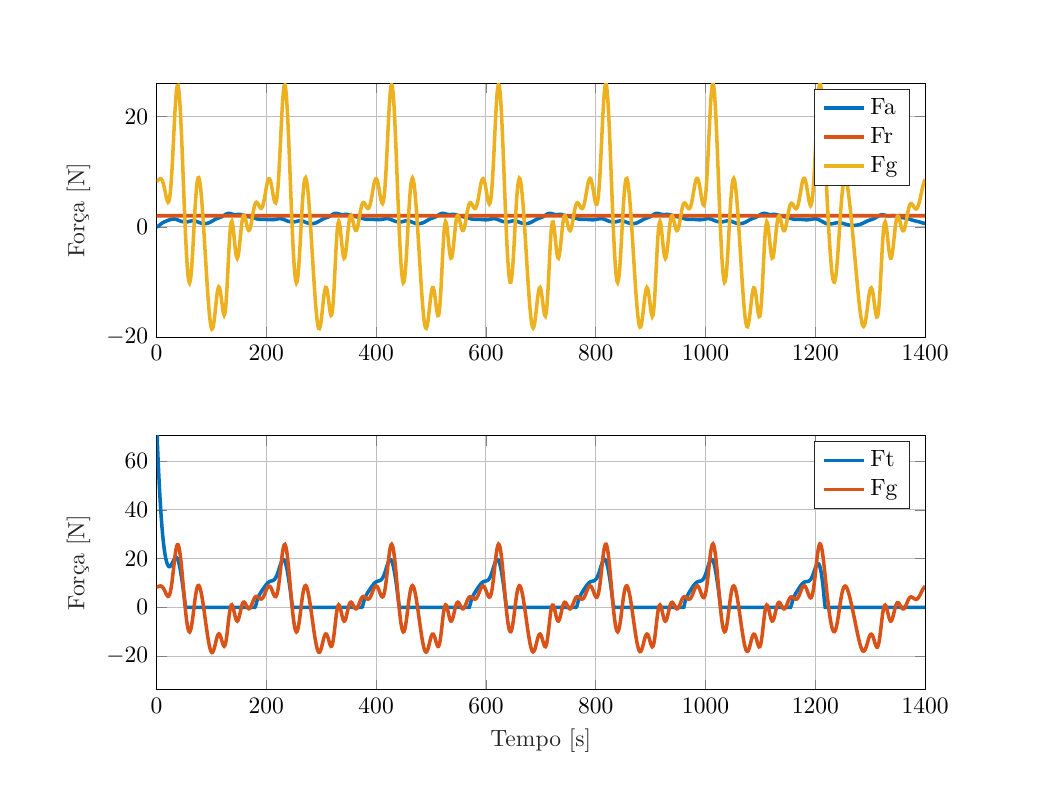
\begin{tikzpicture}[scale=0.85]

\begin{axis}[%
width=4.521in,
height=1.493in,
at={(0.758in,2.554in)},
scale only axis,
xmin=0,
xmax=1400,
ymin=-20,
ymax=26.0142399022586,
ylabel style={font=\color{white!15!black}},
ylabel={Força [N]},
axis background/.style={fill=white},
xmajorgrids,
ymajorgrids,
legend style={legend cell align=left, align=left, draw=white!15!black},
/pgf/number format/.cd,
        use comma,
        1000 sep={}
]
\addplot [color=mycolor1, line width=1.5pt]
  table[row sep=crcr]{%
0	3.217004515581e-49\\
1.4	0.0490879688088317\\
2.8	0.130781775525916\\
4.2	0.233055578508205\\
5.6	0.343887591995691\\
7	0.454827773154235\\
8.4	0.560505704180919\\
9.8	0.658029729004542\\
11.2	0.746380195653321\\
12.6	0.825851260738903\\
14	0.897565115246203\\
15.4	0.963064637818148\\
16.8	1.02398062639117\\
18.2	1.08176504973253\\
19.6	1.13748113822941\\
21	1.19164443154333\\
22.4	1.24411575565368\\
23.8	1.29405599120223\\
25.2	1.33996013996125\\
26.6	1.37978972613638\\
28	1.41121300971989\\
29.4	1.43193976351213\\
30.8	1.4401057373163\\
32.2	1.4346332073638\\
33.6	1.41548367572713\\
35	1.38373732878175\\
36.4	1.3414784270962\\
37.8	1.2915193160459\\
39.2	1.23703587594006\\
40.6	1.18119912937629\\
42	1.12687128102664\\
43.4	1.07640168098763\\
44.8	1.03152444005037\\
46.2	0.993335566688485\\
47.6	0.962317142636569\\
49	0.938377231828012\\
50.4	0.920882716133175\\
51.8	0.908674181124993\\
53.2	0.902139278648554\\
54.6	0.905697341124776\\
56	0.921515759222509\\
57.4	0.947130188793441\\
58.8	0.979720680685086\\
60.2	1.01603788153634\\
61.6	1.05243587481571\\
63	1.08504545372136\\
64.4	1.11009074682197\\
65.8	1.12430723973929\\
67.2	1.12537409499321\\
68.6	1.11224939818127\\
70	1.08531091626266\\
71.4	1.04625784014742\\
72.8	0.997800609283371\\
74.2	0.943225290327933\\
75.6	0.885942446806967\\
77	0.829114235424024\\
78.4	0.775412317209727\\
79.8	0.726914414723899\\
81.2	0.685114895319699\\
82.6	0.651010072397487\\
84	0.625219000242278\\
85.4	0.608108862853309\\
86.8	0.599904593928593\\
88.2	0.600771384780743\\
89.6	0.610864835263063\\
91	0.630346860697087\\
92.4	0.659367083493272\\
93.8	0.698010617065464\\
95.2	0.74621522330011\\
96.6	0.803664930333437\\
98	0.869673934110563\\
99.4	0.943083475755868\\
100.8	1.02220312978874\\
102.2	1.10483224330106\\
103.6	1.18839159278797\\
105	1.27017546240235\\
106.4	1.34770124298641\\
107.8	1.41909625536784\\
109.2	1.48343531209438\\
110.6	1.5409423340124\\
112	1.59299943445149\\
113.4	1.6419561031217\\
114.8	1.69077794362284\\
116.2	1.74259971902441\\
117.6	1.80024579488121\\
119	1.86576278325093\\
120.4	1.9399931896581\\
121.8	2.02222165922803\\
123.2	2.10995170995139\\
124.6	2.19890772850615\\
126	2.28337367233323\\
127.4	2.35693797263637\\
128.8	2.41359319103944\\
130.2	2.44896876925468\\
131.6	2.46134394303901\\
133	2.45209683868693\\
134.4	2.42542633820739\\
135.8	2.38745106639839\\
137.2	2.34499611079864\\
138.6	2.30442157692861\\
140	2.27074052889413\\
141.4	2.24711186552325\\
142.8	2.23467048128779\\
144.2	2.23261193323058\\
145.6	2.2384655882936\\
147	2.24852651608348\\
148.4	2.25843277303613\\
149.8	2.2638523420824\\
151.2	2.26119186548468\\
152.6	2.24819054628123\\
154	2.22425661548196\\
155.4	2.19045972357918\\
156.8	2.14919206829305\\
158.2	2.10360697549651\\
159.6	2.05699161137619\\
161	2.01221687228651\\
162.4	1.9713524546463\\
163.8	1.93547292993568\\
165.2	1.90463692603866\\
166.6	1.87800315099731\\
168	1.85404617512903\\
169.4	1.83083900127001\\
170.8	1.80636950673688\\
172.2	1.77885230888735\\
173.6	1.74699171765588\\
175	1.71015306261581\\
176.4	1.66841384690979\\
177.8	1.62249116790463\\
179.2	1.573569441926\\
180.6	1.52482895431763\\
182	1.48175453262166\\
183.4	1.4469496780908\\
184.8	1.41970857900621\\
186.2	1.39933068773591\\
187.6	1.38503477335671\\
189	1.37591240544514\\
190.4	1.37091605983647\\
191.8	1.36887969127946\\
193.2	1.36857015009124\\
194.6	1.36876595554491\\
196	1.36835591733437\\
197.4	1.36644507457897\\
198.8	1.36245135323023\\
200.2	1.35617533182882\\
201.6	1.3478288352012\\
203	1.33801539956524\\
204.4	1.32766489905554\\
205.8	1.31793280591822\\
207.2	1.31007910592261\\
208.6	1.3053417739334\\
210	1.30481575485505\\
211.4	1.30934274826996\\
212.8	1.31941231169975\\
214.2	1.33507297794379\\
215.6	1.35585436584673\\
217	1.3807075603002\\
218.4	1.40797978110118\\
219.8	1.43544726645794\\
221.2	1.46043249721296\\
222.6	1.48002316297706\\
224	1.49138784696333\\
225.4	1.49215055428582\\
226.8	1.48075409928686\\
228.2	1.4567270173738\\
229.6	1.42078244852604\\
231	1.37471980915104\\
232.4	1.32115511744215\\
233.8	1.26315030020376\\
235.2	1.20382846036313\\
236.6	1.14604859725821\\
238	1.09218084117975\\
239.4	1.0439879010806\\
240.8	1.00259228491498\\
242.2	0.968496558919122\\
243.6	0.941624001059492\\
245	0.921354920460427\\
246.4	0.90654598376013\\
247.8	0.897231677265483\\
249.2	0.897933823700329\\
250.6	0.911308560094428\\
252	0.934974527679672\\
253.4	0.966225175296341\\
254.8	1.00193787184596\\
256.2	1.03857865355668\\
257.6	1.07234029249674\\
259	1.09942484573279\\
260.4	1.11644001470232\\
261.8	1.12083259855698\\
263.2	1.11125187969613\\
264.6	1.08774002748103\\
266	1.05169083180343\\
267.4	1.00558684784822\\
268.8	0.952588917390007\\
270.2	0.896084615900929\\
271.6	0.839294751516557\\
273	0.785000562751293\\
274.4	0.735409330243681\\
275.8	0.692140380100269\\
277.2	0.65629477504817\\
278.6	0.628569040677276\\
280	0.609380067427227\\
281.4	0.598978584072025\\
282.8	0.597538047311349\\
284.2	0.605212543211554\\
285.6	0.622161213600318\\
287	0.648538637590064\\
288.4	0.684451749635163\\
289.8	0.729885576913688\\
291.2	0.784603514828632\\
292.6	0.848033792596019\\
294	0.919162059710408\\
295.4	0.996458938901234\\
296.8	1.07787723307723\\
298.2	1.16095098106737\\
299.6	1.24301294768732\\
301	1.32151764182267\\
302.4	1.39442015343627\\
303.8	1.46053087037514\\
305.2	1.51975803316717\\
306.6	1.57317188773924\\
308	1.62286906491062\\
309.4	1.67166447033276\\
310.8	1.72266976822943\\
312.2	1.7788228283068\\
313.6	1.84241751342896\\
315	1.91466515157037\\
316.4	1.99531590705746\\
317.8	2.08238871360933\\
319.2	2.172094947548\\
320.6	2.25906757125864\\
322	2.33698595842664\\
323.4	2.39958800039438\\
324.8	2.44189792809525\\
326.2	2.4613439440568\\
327.6	2.45839987306954\\
329	2.4365195566298\\
330.4	2.40139010568436\\
331.8	2.35976936580539\\
333.2	2.31826791795336\\
334.6	2.28236528493959\\
336	2.25579263159054\\
337.4	2.2402726530016\\
338.8	2.23553912629453\\
340.2	2.23956121590181\\
341.6	2.24893279398666\\
343	2.25941204269292\\
344.4	2.26658548021079\\
345.8	2.26658425661446\\
347.2	2.25672666179359\\
348.6	2.23593956817969\\
350	2.2048504484813\\
351.4	2.16553309293563\\
352.8	2.12099250204321\\
354.2	2.07453889231323\\
355.6	2.02920348505505\\
357	1.9873018468976\\
358.4	1.95018700488218\\
359.8	1.91818412049439\\
361.2	1.89067335645009\\
362.6	1.86628302953259\\
364	1.84315889519891\\
365.4	1.81927687496107\\
366.8	1.79276209325214\\
368.2	1.76217050759835\\
369.6	1.72668845202317\\
371	1.68621636719799\\
372.4	1.64132603273417\\
373.8	1.59310882259306\\
375.2	1.54367502334901\\
376.6	1.49879074447124\\
378	1.46232941877875\\
379.4	1.43357701366229\\
380.8	1.41184647791308\\
382.2	1.39638148309086\\
383.6	1.38630121935007\\
385	1.38058124227181\\
386.4	1.37806783803649\\
387.8	1.37752436000072\\
389.2	1.37770656765661\\
390.6	1.37746024452382\\
392	1.3758292697369\\
393.4	1.37215775415552\\
394.8	1.36616804338374\\
396.2	1.357998912149\\
397.6	1.34819513624361\\
399	1.33764899429353\\
400.4	1.32750311349151\\
401.8	1.31902958617327\\
403.2	1.3135010289584\\
404.6	1.31206574968961\\
406	1.31563347598547\\
407.4	1.32477281922025\\
408.8	1.3396191015961\\
410.2	1.35979273922856\\
411.6	1.38433419998156\\
413	1.41167031777802\\
414.4	1.43963537782909\\
415.8	1.46557409720952\\
417.2	1.48654691686326\\
418.6	1.49963732358584\\
420	1.50232832543142\\
421.4	1.49288094632726\\
422.8	1.4706279044298\\
424.2	1.43610462314747\\
425.6	1.39097940268119\\
427	1.33780071338976\\
428.4	1.27962840613601\\
429.8	1.2196375979476\\
431.2	1.1607742058488\\
432.6	1.10550955893044\\
434	1.05570467675635\\
435.4	1.01256615051254\\
436.8	0.976661180501937\\
438.2	0.947957770980275\\
439.6	0.925863267635798\\
441	0.909247965137211\\
442.4	0.897985924547965\\
443.8	0.89673656259027\\
445.2	0.908460945490687\\
446.6	0.930807524151214\\
448	0.961118641615345\\
449.4	0.996330811415281\\
450.8	1.03296444278016\\
452.2	1.06724269178107\\
453.6	1.09535487477704\\
455	1.11383981829916\\
456.4	1.12001827305928\\
457.8	1.11237004031996\\
459.2	1.09075053982227\\
460.6	1.05638081995771\\
462	1.01161172609476\\
463.4	0.959528827506816\\
464.8	0.903502117307262\\
466.2	0.846782075623498\\
467.6	0.792210129980649\\
469	0.742066825660679\\
470.4	0.698043603134046\\
471.8	0.661303166639855\\
473.2	0.632588695506585\\
474.6	0.612347985116149\\
476	0.600848629222842\\
477.4	0.598270010883508\\
478.8	0.604764986000653\\
480.2	0.620488401043811\\
481.6	0.64559172426805\\
483	0.680184284642249\\
484.4	0.724263211910799\\
485.8	0.777617352401123\\
487.2	0.839716012980586\\
488.6	0.909601330665341\\
490	0.985811881200355\\
491.4	1.06637138849152\\
492.8	1.148875015514\\
494.2	1.23069183281692\\
495.6	1.30927433991343\\
497	1.38252996056174\\
498.4	1.44917824756047\\
499.8	1.50900659615542\\
501.2	1.56295546279035\\
502.6	1.61300638642624\\
504	1.66189456249909\\
505.4	1.71270158304593\\
506.8	1.76839211264801\\
508.2	1.83134514246005\\
509.6	1.90291222863551\\
511	1.98302993873926\\
512.4	2.06993168504296\\
513.8	2.16003992972101\\
515.2	2.24814961826386\\
516.6	2.32800024707235\\
518	2.39324532299411\\
519.4	2.43866973977394\\
520.8	2.46134392798294\\
522.2	2.46134394419129\\
523.6	2.44177960803518\\
525	2.4081219034994\\
526.4	2.36707134923933\\
527.8	2.32532622560347\\
529.2	2.28855683431883\\
530.6	2.26073924576457\\
532	2.24385367392137\\
533.4	2.23787406382356\\
534.8	2.24097081574206\\
536.2	2.24988208891091\\
537.6	2.26043717241661\\
539	2.26820918344423\\
540.4	2.26923134745874\\
541.8	2.26065616759548\\
543.2	2.24120987964002\\
544.6	2.21132609131471\\
546	2.17292949127897\\
547.4	2.12894428442198\\
548.8	2.08267281835957\\
550.2	2.03719984077815\\
551.6	1.99493523405949\\
553	1.95734472401931\\
554.4	1.92486510150012\\
555.8	1.89697236044412\\
557.2	1.87236472074737\\
558.6	1.84922580673496\\
560	1.82553517706618\\
561.4	1.79938947001746\\
562.8	1.76929073636015\\
564.2	1.73435667476406\\
565.6	1.69441717609935\\
567	1.64998373326835\\
568.4	1.60210654251137\\
569.8	1.55215818187574\\
571.2	1.50499247360152\\
572.6	1.46556183896041\\
574	1.434352370567\\
575.4	1.410575928674\\
576.8	1.39340426843404\\
578.2	1.38190670699839\\
579.6	1.3750249620882\\
581	1.3715818807614\\
582.4	1.3703222709777\\
583.8	1.36998301578139\\
585.2	1.36938622036607\\
586.6	1.36754422676741\\
588	1.36376072335163\\
589.4	1.35771005941542\\
590.8	1.34947889909947\\
592.2	1.33956070346448\\
593.6	1.32880259099484\\
595	1.31831301905964\\
596.4	1.30934458698715\\
597.8	1.303167504465\\
599.2	1.30094619278767\\
600.6	1.30362595619972\\
602	1.31183122877556\\
603.4	1.32577389146615\\
604.8	1.34517105035209\\
606.2	1.36917681621375\\
607.6	1.39634100611266\\
609	1.42461663229746\\
610.4	1.45144313894805\\
611.8	1.47392816778385\\
613.2	1.48913299623744\\
614.6	1.49443634483556\\
616	1.48791644358029\\
617.4	1.46866736916538\\
618.8	1.4369679583574\\
620.2	1.39425518304759\\
621.6	1.34290783451602\\
623	1.2858981924093\\
624.4	1.22639771612605\\
625.8	1.16741940311987\\
627.2	1.11155152380958\\
628.6	1.06080085826447\\
630	1.01653273851747\\
631.4	0.979477359808519\\
632.8	0.949767870354855\\
634.2	0.926981754241972\\
635.6	0.910168913602748\\
637	0.89786089108065\\
638.4	0.89375400624464\\
639.8	0.902222570989493\\
641.2	0.921917361627733\\
642.6	0.950276901320103\\
644	0.984357235166016\\
645.4	1.02079431320999\\
646.8	1.05588608039636\\
648.2	1.08581730182449\\
649.6	1.10701402357713\\
651	1.11656887193212\\
652.4	1.11263997566227\\
653.8	1.09471565910583\\
655.2	1.06366597764326\\
656.6	1.02156339775183\\
658	0.971323291021336\\
659.4	0.916261209487622\\
660.8	0.859671766582615\\
662.2	0.80450719615891\\
663.6	0.753190332704164\\
665	0.707556520219578\\
666.4	0.668893625970231\\
667.8	0.638040787845232\\
669.2	0.615510134568422\\
670.6	0.601605052297786\\
672	0.596518523438371\\
673.4	0.600402880938687\\
674.8	0.61340727025387\\
676.2	0.635681704759425\\
677.6	0.667347936118895\\
679	0.70843871636437\\
680.4	0.758809626711501\\
681.8	0.818032422132498\\
683.2	0.885286040693242\\
684.6	0.959270043741743\\
686	1.03817247301239\\
687.4	1.11972533934111\\
688.8	1.20137113247776\\
690.2	1.28054023593803\\
691.6	1.35500527658837\\
693	1.42324508681964\\
694.4	1.48473326794718\\
695.8	1.54007572899001\\
697.2	1.59095738069369\\
698.6	1.63990588718189\\
700	1.68991931178632\\
701.4	1.74402007355961\\
702.8	1.80478969040199\\
704.2	1.87392055464713\\
705.6	1.9518107578427\\
707	2.0372389444218\\
708.4	2.12718829463205\\
709.8	2.21692410802398\\
711.2	2.30043391071005\\
712.6	2.37127607558174\\
714	2.4237428371308\\
715.4	2.45407267368901\\
716.8	2.46134394387241\\
718.2	2.44773749173672\\
719.6	2.41807242758206\\
721	2.37878580782354\\
722.4	2.33669614339831\\
723.8	2.29788878998539\\
725.2	2.26692936789708\\
726.6	2.2464520486906\\
728	2.23706564266465\\
729.4	2.23749471216885\\
730.8	2.24489900330221\\
732.2	2.25534832539174\\
733.6	2.2644364661564\\
735	2.26798528553683\\
736.4	2.26273536939445\\
737.8	2.2468796584974\\
739.2	2.22030756593312\\
740.6	2.18449860077978\\
742	2.14210787642539\\
743.4	2.09637146288436\\
744.8	2.05048980080351\\
746.2	2.00711916786675\\
747.6	1.96804102989639\\
749	1.93402059104448\\
750.4	1.90482947921585\\
751.8	1.87939514094468\\
753.2	1.85604099684492\\
754.6	1.83278455888469\\
756	1.80765863674647\\
757.4	1.77901428742338\\
758.8	1.74575991975593\\
760.2	1.70749652408658\\
761.6	1.66452747559153\\
763	1.6177486166144\\
764.4	1.56845074814404\\
765.8	1.51962532318273\\
767.2	1.47671351394065\\
768.6	1.44243052876152\\
770	1.41594435073781\\
771.4	1.39641901197391\\
772.8	1.38293794527503\\
774.2	1.37446649159653\\
775.6	1.36984917958591\\
777	1.36783971698652\\
778.4	1.36716145346397\\
779.8	1.36659338423066\\
781.2	1.3650721903258\\
782.6	1.36179589322178\\
784	1.35631157569179\\
785.4	1.34857021266838\\
786.8	1.33893669725595\\
788.2	1.32815158549878\\
789.6	1.31725034157974\\
791	1.30745293147073\\
792.4	1.30003939155908\\
793.8	1.29622516874644\\
795.2	1.29704501510309\\
796.6	1.30324844536057\\
798	1.31520569671492\\
799.4	1.33282256719539\\
800.8	1.35546621135679\\
802.2	1.38191144534794\\
803.6	1.41032634257671\\
805	1.43832311538551\\
806.4	1.463100263124\\
807.8	1.48168968782996\\
809.2	1.49129629021725\\
810.6	1.48968277708963\\
812	1.47552224708166\\
813.4	1.4486320275059\\
814.8	1.41002432641227\\
816.2	1.36175783057743\\
817.6	1.30663006329785\\
819	1.24778957528341\\
820.4	1.18835567613923\\
821.8	1.13111310592367\\
823.2	1.07831392349155\\
824.6	1.03158421054587\\
826	0.991909937626726\\
827.4	0.959667684735958\\
828.8	0.934668288704382\\
830.2	0.916192122435801\\
831.6	0.903005553904164\\
833	0.895816347741114\\
834.4	0.899017998980026\\
835.8	0.914403948349531\\
837.2	0.939522046414183\\
838.6	0.971578389021977\\
840	1.00736430997443\\
841.4	1.04328788522436\\
842.8	1.07554251054312\\
844.2	1.10041505836791\\
845.6	1.11469267834662\\
847	1.11608374552275\\
848.4	1.10354506709478\\
849.8	1.07742086472048\\
851.2	1.03934993356971\\
852.6	0.991966444006063\\
854	0.938477399738228\\
855.4	0.882222972950096\\
856.8	0.826310928235044\\
858.2	0.773377007134074\\
859.6	0.725479905589956\\
861	0.684107777985341\\
862.4	0.650258530085224\\
863.8	0.624555836305956\\
865.2	0.607370631549638\\
866.6	0.598927962422081\\
868	0.599387879963396\\
869.4	0.608895095169931\\
870.8	0.627595525017898\\
872.2	0.655619563015139\\
873.6	0.693033151554456\\
875	0.739759771077541\\
876.4	0.795480352478306\\
877.8	0.859524403119087\\
879.2	0.930773821863775\\
880.6	1.00760885802696\\
882	1.08792947903158\\
883.4	1.16928000853597\\
884.8	1.24908648292916\\
886.2	1.3249856385033\\
887.6	1.39518990336318\\
889	1.45880828638801\\
890.4	1.51604215529193\\
891.8	1.56820178278923\\
893.2	1.61753444226525\\
894.6	1.66689832880045\\
896	1.71934093737156\\
897.4	1.77764012707\\
898.8	1.84384985882844\\
900.2	1.91887787350834\\
901.6	2.00212528825601\\
903	2.0912437290216\\
904.4	2.18210320061693\\
905.8	2.26908458790958\\
907.2	2.34577628007116\\
908.6	2.40604112919998\\
910	2.44525093525268\\
911.4	2.46134394331387\\
912.8	2.45535038619901\\
914.2	2.43119491700549\\
915.6	2.39485053463281\\
917	2.35313914800954\\
918.4	2.31253743932026\\
919.8	2.2782530126769\\
921.2	2.25367446243037\\
922.6	2.24016809667458\\
924	2.23713996592075\\
925.4	2.24229327796424\\
926.8	2.25204711931839\\
928.2	2.26210186970733\\
929.6	2.26811839648204\\
931	2.26642830454653\\
932.4	2.25464240672718\\
933.8	2.23201380329988\\
935.2	2.19946233164518\\
936.6	2.15926377340464\\
938	2.11450487855362\\
939.4	2.06845832506505\\
940.8	2.02402335554592\\
942.2	1.9833256009089\\
943.6	1.94750727354658\\
945	1.91669325567545\\
946.4	1.89009809255441\\
947.8	1.86623667114614\\
949.2	1.84320496151444\\
950.6	1.81899727402226\\
952	1.7918210623953\\
953.4	1.76036433677423\\
954.8	1.72397211713066\\
956.2	1.68270229832917\\
957.6	1.63725633476341\\
959	1.58880814692677\\
960.4	1.53882183903324\\
961.8	1.4931428220414\\
963.2	1.45632003192013\\
964.6	1.42752273268242\\
966	1.40593855766477\\
967.4	1.390692279739\\
968.8	1.38079559675332\\
970.2	1.37513305694885\\
971.6	1.3724816264063\\
973	1.37156204631351\\
974.4	1.37111820283895\\
975.8	1.37001658361859\\
977.2	1.3673527758454\\
978.6	1.36254791211264\\
980	1.35541714008927\\
981.4	1.34619583553321\\
982.8	1.33551694849791\\
984.2	1.32434236755864\\
985.6	1.31385942250358\\
987	1.30535803745758\\
988.4	1.3001036261495\\
989.8	1.29921651597999\\
991.2	1.30356274402495\\
992.6	1.31365608444315\\
994	1.32956925629509\\
995.4	1.35085457391172\\
996.8	1.37648078859719\\
998.2	1.40480203894829\\
999.6	1.43358345101771\\
1001	1.46011108349934\\
1002.4	1.48140609354159\\
1003.8	1.49454090455737\\
1005.2	1.49702149738091\\
1006.6	1.48716572338322\\
1008	1.4643893922873\\
1009.4	1.42932352388458\\
1010.8	1.38372832708696\\
1012.2	1.33022658181874\\
1013.6	1.27192687596443\\
1015	1.21202670535626\\
1016.4	1.15347322080264\\
1017.8	1.09872646632619\\
1019.2	1.04963296176288\\
1020.6	1.00738972376767\\
1022	0.972565128552919\\
1023.4	0.945142336381971\\
1024.8	0.924559596170527\\
1026.2	0.909733576986112\\
1027.6	0.899461127297126\\
1029	0.898241232356867\\
1030.4	0.909949432655424\\
1031.8	0.932202078600384\\
1033.2	0.962312077149133\\
1034.6	0.997193198990394\\
1036	1.03335549811009\\
1037.4	1.06703024235223\\
1038.8	1.09443759795278\\
1040.2	1.11217001829904\\
1041.6	1.11761888460309\\
1043	1.10934040501058\\
1044.4	1.087258169573\\
1045.8	1.05264049857598\\
1047.2	1.00785713538638\\
1048.6	0.955983723281916\\
1050	0.900357307271833\\
1051.4	0.844181770966104\\
1052.8	0.790248073394169\\
1054.2	0.740790185016874\\
1055.6	0.697461505012993\\
1057	0.66139678773205\\
1058.4	0.633320548020297\\
1059.8	0.61366893649352\\
1061.2	0.602701974399328\\
1062.6	0.600592452643817\\
1064	0.607484700807726\\
1065.4	0.623520568154384\\
1066.8	0.648832086544017\\
1068.2	0.683501587570365\\
1069.6	0.727491791807014\\
1071	0.780551706039444\\
1072.4	0.84210976179845\\
1073.8	0.91117333470471\\
1075.2	0.986261971760945\\
1076.6	1.06540686486887\\
1078	1.1462465051091\\
1079.4	1.22623370196012\\
1080.8	1.30294164809888\\
1082.2	1.37442255044599\\
1083.6	1.43954426156315\\
1085	1.49822257101679\\
1086.4	1.5514865550007\\
1087.8	1.60135556315529\\
1089.2	1.65055153009168\\
1090.6	1.70210031049645\\
1092	1.75888140679176\\
1093.4	1.82317212113322\\
1094.8	1.89621564134378\\
1096.2	1.97783991770127\\
1097.6	2.06617431609531\\
1099	2.15754778465786\\
1100.4	2.24668136551437\\
1101.8	2.32727195902218\\
1103.2	2.39297234410418\\
1104.6	2.43861214163941\\
1106	2.46134393810739\\
1107.4	2.46134394102386\\
1108.8	2.44181537229313\\
1110.2	2.40829477475558\\
1111.6	2.3675096589596\\
1113	2.32614761435776\\
1114.4	2.28983949382548\\
1115.8	2.26250502347045\\
1117.2	2.24606234902968\\
1118.6	2.24042698859661\\
1120	2.24372271515001\\
1121.4	2.25266055106669\\
1122.8	2.26306893087034\\
1124.2	2.27055032350626\\
1125.6	2.27119590631287\\
1127	2.26223597560251\\
1128.4	2.24247951793354\\
1129.8	2.21243076277766\\
1131.2	2.17405882242079\\
1132.6	2.1302990736034\\
1134	2.08443276653322\\
1135.4	2.03949841700843\\
1136.8	1.99784458184146\\
1138.2	1.96087066903484\\
1139.6	1.92895082596336\\
1141	1.90150907319912\\
1142.4	1.87720795811078\\
1143.8	1.85421608090574\\
1145.2	1.83052115688945\\
1146.6	1.80425088485326\\
1148	1.77395733123369\\
1149.4	1.73881951704685\\
1150.8	1.6987298006308\\
1152.2	1.65425278045249\\
1153.6	1.60647391539292\\
1155	1.5567784022552\\
1156.4	1.50926183595118\\
1157.8	1.46898977730008\\
1159.2	1.43724519147385\\
1160.6	1.41314589853844\\
1162	1.39577658385686\\
1163.4	1.38412728377275\\
1164.8	1.37706982535318\\
1166.2	1.37336885225437\\
1167.6	1.37172547152525\\
1169	1.37085024210445\\
1170.4	1.36955849576004\\
1171.8	1.36687592466284\\
1173.2	1.36213791928264\\
1174.6	1.35506450865043\\
1176	1.34579546659691\\
1177.4	1.33487714045094\\
1178.8	1.32320194394356\\
1180.2	1.31191021880619\\
1181.6	1.30226950715418\\
1183	1.29554683365873\\
1184.4	1.2928859349362\\
1185.8	1.29519554323046\\
1187.2	1.30304943188083\\
1188.6	1.31659621378116\\
1190	1.33547820727142\\
1191.4	1.35876424886409\\
1192.8	1.3849099779933\\
1194.2	1.41176804407319\\
1195.6	1.43667537279265\\
1197	1.45663964992383\\
1198.4	1.46862855656133\\
1199.8	1.46993411284164\\
1201.2	1.45854974832747\\
1202.6	1.43347499041079\\
1204	1.39486687306528\\
1205.4	1.34399253995919\\
1206.8	1.28299219657902\\
1208.2	1.21451271910668\\
1209.6	1.14129911471821\\
1211	1.06582647505711\\
1212.4	0.990027265608293\\
1213.8	0.915133929535841\\
1215.2	0.841629046581776\\
1216.6	0.769282493707002\\
1218	0.699967895897607\\
1219.4	0.64117300069\\
1220.8	0.59712573482796\\
1222.2	0.566068051695489\\
1223.6	0.546466580232335\\
1225	0.537014002022493\\
1226.4	0.536588099868007\\
1227.8	0.544183133493219\\
1229.2	0.558824441896298\\
1230.6	0.579475885660792\\
1232	0.604950750068486\\
1233.4	0.633839245686851\\
1234.8	0.664468339734478\\
1236.2	0.694910300680079\\
1237.6	0.723052796196207\\
1239	0.7467340873226\\
1240.4	0.763932174102399\\
1241.8	0.772979915572406\\
1243.2	0.772765004967543\\
1244.6	0.762870540769839\\
1246	0.743622261803604\\
1247.4	0.716030316934936\\
1248.8	0.681639408150539\\
1250.2	0.64232196433866\\
1251.6	0.600057914150907\\
1253	0.55674036383747\\
1254.4	0.514032975121947\\
1255.8	0.473288390703783\\
1257.2	0.435523179233989\\
1258.6	0.401436342944632\\
1260	0.371455623534742\\
1261.4	0.345797151015625\\
1262.8	0.32452742332871\\
1264.2	0.307620531213044\\
1265.6	0.29500694069259\\
1267	0.286612593303038\\
1268.4	0.282388555967514\\
1269.8	0.282332118222475\\
1271.2	0.286500319038661\\
1272.6	0.29501659418105\\
1274	0.308070730752185\\
1275.4	0.325911726541357\\
1276.8	0.348832595681362\\
1278.2	0.377145775359907\\
1279.6	0.411147752596044\\
1281	0.451072083845314\\
1282.4	0.497031397680555\\
1283.8	0.548951484253114\\
1285.2	0.606504219636866\\
1286.6	0.669050459186662\\
1288	0.735608118273695\\
1289.4	0.804862672700855\\
1290.8	0.875235080213186\\
1292.2	0.945013944054681\\
1293.6	1.01254466882364\\
1295	1.07645129627394\\
1296.4	1.13585226082165\\
1297.8	1.19052579576187\\
1299.2	1.24098789050274\\
1300.6	1.28846399971717\\
1302	1.33475832905624\\
1303.4	1.38204265477548\\
1304.8	1.43259409817768\\
1306.2	1.48850768331247\\
1307.6	1.55140025102096\\
1309	1.62211586898697\\
1310.4	1.70044711574243\\
1311.8	1.78490510722198\\
1313.2	1.87259983518028\\
1314.6	1.9593171429806\\
1316	2.03987638546698\\
1317.4	2.10880089446432\\
1318.8	2.1612284466654\\
1320.2	2.19386492082985\\
1321.6	2.20570856857393\\
1323	2.19830691754037\\
1324.4	2.17545764970416\\
1325.8	2.14245809945305\\
1327.2	2.10514400121263\\
1328.6	2.06897677087259\\
1330	2.03835605330545\\
1331.4	2.01621658231579\\
1332.8	2.00387877509567\\
1334.2	2.00108785798458\\
1335.6	2.00618744844627\\
1337	2.01640313825613\\
1338.4	2.02823233014679\\
1339.8	2.03793168120014\\
1341.2	2.042062317918\\
1342.6	2.03801150715138\\
1344	2.02438400552478\\
1345.4	2.00116921776517\\
1346.8	1.9696444014835\\
1348.2	1.93204798391437\\
1349.6	1.89111702261395\\
1351	1.84960432121684\\
1352.4	1.80987160648075\\
1353.8	1.77361290329906\\
1355.2	1.74171955714037\\
1356.6	1.7142702593124\\
1358	1.69061880536346\\
1359.4	1.66955328259332\\
1360.8	1.64950446821483\\
1362.2	1.62878229766122\\
1363.6	1.605815834951\\
1365	1.57936715070333\\
1366.4	1.54868804723188\\
1367.8	1.51359488976385\\
1369.2	1.47445142738034\\
1370.6	1.43206846522711\\
1372	1.38754603810349\\
1373.4	1.34209263426528\\
1374.8	1.29685496496405\\
1376.2	1.25278285659089\\
1377.6	1.21054157903611\\
1379	1.17047277123775\\
1380.4	1.13259771719411\\
1381.8	1.09665349007933\\
1383.2	1.06215229868738\\
1384.6	1.02845558079929\\
1386	0.994855611069159\\
1387.4	0.960657938803295\\
1388.8	0.925257893437442\\
1390.2	0.888204264543273\\
1391.6	0.849243814063878\\
1393	0.808342027138846\\
1394.4	0.765678474671207\\
1395.8	0.721618812066974\\
1397.2	0.676668879095916\\
1398.6	0.631418697092965\\
1400	0.586484833015212\\
};
\addlegendentry{Fa}

\addplot [color=mycolor2, line width=1.5pt]
  table[row sep=crcr]{%
0	2.02468540454964\\
1.4	2.02468439025944\\
2.8	2.02468193790584\\
4.2	2.0246789971254\\
5.6	2.02467642156008\\
7	2.02467518204898\\
8.4	2.02467622554373\\
9.8	2.02468027463496\\
11.2	2.02468761404093\\
12.6	2.02469793853008\\
14	2.02471033556406\\
15.4	2.0247234381143\\
16.8	2.02473571683463\\
18.2	2.02474580754565\\
19.6	2.02475271748622\\
21	2.02475575002959\\
22.4	2.02475405725698\\
23.8	2.02474588628519\\
25.2	2.02472780988373\\
26.6	2.02469444453637\\
28	2.02463920881163\\
29.4	2.02455639817352\\
30.8	2.02444421586959\\
32.2	2.02430764589473\\
33.6	2.0241596725921\\
35	2.02401976751468\\
36.4	2.02390972810282\\
37.8	2.02384823893715\\
39.2	2.02384614685027\\
40.6	2.02390404845875\\
42	2.02401270708367\\
43.4	2.02415572337239\\
44.8	2.02431329905488\\
46.2	2.02446595360659\\
47.6	2.02459744890899\\
49	2.02469663872522\\
50.4	2.02475828415234\\
51.8	2.02478300914383\\
53.2	2.02477655195381\\
54.6	2.0247483350157\\
56	2.0247096478098\\
57.4	2.02467201025126\\
58.8	2.02464557459498\\
60.2	2.02463735074515\\
61.6	2.02464960290788\\
63	2.02467903619163\\
64.4	2.02471740291583\\
65.8	2.02475376077427\\
67.2	2.02477787566375\\
68.6	2.02478355893035\\
70	2.02477056425271\\
71.4	2.02474426798997\\
72.8	2.02471340581111\\
74.2	2.0246869852763\\
75.6	2.0246716598554\\
77	2.02467036683258\\
78.4	2.02468231957674\\
79.8	2.02470392842985\\
81.2	2.02473007083505\\
82.6	2.02475525723944\\
84	2.02477446877346\\
85.4	2.02478364018566\\
86.8	2.02477987373436\\
88.2	2.02476150331362\\
89.6	2.0247281119927\\
91	2.02468056671189\\
92.4	2.02462108637376\\
93.8	2.02455331038073\\
95.2	2.02448228785844\\
96.6	2.02441427229664\\
98	2.02435620079443\\
99.4	2.02431478814399\\
100.8	2.02429529428932\\
102.2	2.0243002164314\\
103.6	2.02432833985241\\
105	2.02437462277074\\
106.4	2.02443117178589\\
107.8	2.02448910209548\\
109.2	2.02454059510698\\
110.6	2.02458030010769\\
112	2.02460556342716\\
113.4	2.02461564425384\\
114.8	2.024610658001\\
116.2	2.0245910998563\\
117.6	2.02455839021623\\
119	2.02451620120285\\
120.4	2.02447170925816\\
121.8	2.02443564149604\\
123.2	2.02442023462976\\
124.6	2.02443512313043\\
126	2.02448257936115\\
127.4	2.02455474403815\\
128.8	2.0246353213968\\
130.2	2.02470594166524\\
131.6	2.02475406823577\\
133	2.02477767836614\\
134.4	2.02478390754006\\
135.8	2.0247830867067\\
137.2	2.02478250737725\\
138.6	2.02478363781742\\
140	2.02478353713405\\
141.4	2.02477856586538\\
142.8	2.02476772681128\\
144.2	2.02475383699208\\
145.6	2.02474221082315\\
147	2.02473782219962\\
148.4	2.02474260091871\\
149.8	2.02475439673174\\
151.2	2.02476820174373\\
152.6	2.02477887390402\\
154	2.02478368284588\\
155.4	2.02478319795048\\
156.8	2.02478023260107\\
158.2	2.02477781562678\\
159.6	2.02477756719315\\
161	2.02477929213382\\
162.4	2.02478168293222\\
163.8	2.02478342832984\\
165.2	2.02478399876875\\
166.6	2.02478375117462\\
168	2.02478344819149\\
169.4	2.02478358462034\\
170.8	2.02478395768477\\
172.2	2.02478372854378\\
173.6	2.02478191597371\\
175	2.02477801053148\\
176.4	2.02477234296595\\
177.8	2.02476600784585\\
179.2	2.02476041270078\\
180.6	2.02475671693948\\
182	2.0247554452273\\
183.4	2.02475641787683\\
184.8	2.02475893891862\\
186.2	2.02476209462379\\
187.6	2.02476502825049\\
189	2.02476709293409\\
190.4	2.02476785025724\\
191.8	2.02476695503742\\
193.2	2.02476402080048\\
194.6	2.0247585748123\\
196	2.02475017470267\\
197.4	2.02473867711646\\
198.8	2.02472455363169\\
200.2	2.02470908912947\\
201.6	2.02469431485915\\
203	2.02468262831587\\
204.4	2.02467619236505\\
205.8	2.024676316542\\
207.2	2.02468304731751\\
208.6	2.02469512071772\\
210	2.02471029670179\\
211.4	2.02472595708481\\
212.8	2.02473975344088\\
214.2	2.02475005945762\\
215.6	2.02475601756132\\
217	2.02475707438361\\
218.4	2.02475207827706\\
219.8	2.02473825230825\\
221.2	2.02471059159199\\
222.6	2.02466232058129\\
224	2.02458680607968\\
225.4	2.02448068413539\\
226.8	2.02434712925083\\
228.2	2.0241976700152\\
229.6	2.02405123792112\\
231	2.02393027805227\\
232.4	2.02385516410442\\
233.8	2.02383898416823\\
235.2	2.0238845192972\\
236.6	2.02398416733521\\
238	2.02412236933267\\
239.4	2.02427937923455\\
240.8	2.02443515089697\\
242.2	2.0245724922896\\
243.6	2.02467912672736\\
245	2.02474866901216\\
246.4	2.02478069280375\\
247.8	2.02478006915209\\
249.2	2.02475561599112\\
250.6	2.02471830018354\\
252	2.024679617204\\
253.4	2.02465006727327\\
254.8	2.02463743132428\\
256.2	2.02464510945708\\
257.6	2.02467108657201\\
259	2.02470817361363\\
260.4	2.02474587794975\\
261.8	2.02477358473652\\
263.2	2.02478398846429\\
264.6	2.02477539486989\\
266	2.02475193472481\\
267.4	2.02472170925227\\
268.8	2.02469382086882\\
270.2	2.02467558053927\\
271.6	2.0246708319681\\
273	2.02467964464067\\
274.4	2.0246990491376\\
275.8	2.02472425160871\\
277.2	2.02474983598814\\
278.6	2.02477067763573\\
280	2.02478250122886\\
281.4	2.02478214749713\\
282.8	2.0247676632296\\
284.2	2.02473832269425\\
285.6	2.02469465390745\\
287	2.02463849782892\\
288.4	2.02457308048501\\
289.8	2.02450303112958\\
291.2	2.0244342407537\\
292.6	2.02437344010655\\
294	2.02432740951428\\
295.4	2.02430183781364\\
296.8	2.02430002357234\\
298.2	2.02432180327623\\
299.6	2.02436318131078\\
301	2.02441699643515\\
302.4	2.02447455897779\\
303.8	2.02452769731332\\
305.2	2.02457037838617\\
306.6	2.0245992626319\\
308	2.02461315819228\\
309.4	2.0246119778091\\
310.8	2.0245960585189\\
312.2	2.02456642906669\\
313.6	2.02452598101299\\
315	2.02448084492101\\
316.4	2.02444088160935\\
317.8	2.02441827886547\\
319.2	2.0244239475163\\
320.6	2.02446270902553\\
322	2.02452964752474\\
323.4	2.02461035872907\\
324.8	2.02468615529786\\
326.2	2.0247420278372\\
327.6	2.02477272349782\\
329	2.02478319268592\\
330.4	2.0247835743273\\
331.8	2.02478254877882\\
333.2	2.02478331905883\\
334.6	2.02478391534217\\
336	2.02478052175929\\
337.4	2.02477116907583\\
338.8	2.02475762973772\\
340.2	2.02474476130948\\
341.6	2.02473794815281\\
343	2.02474018077186\\
344.4	2.0247504335529\\
345.8	2.02476426862945\\
347.2	2.02477628431016\\
348.6	2.02478289203472\\
350	2.02478375962224\\
351.4	2.02478124570883\\
352.8	2.02477850355123\\
354.2	2.02477762931631\\
355.6	2.02477889420713\\
357	2.02478119755997\\
358.4	2.02478314377547\\
359.8	2.02478396780844\\
361.2	2.02478382883068\\
362.6	2.02478345328709\\
364	2.02478346540736\\
365.4	2.02478385800041\\
366.8	2.02478391979847\\
368.2	2.02478264200984\\
369.6	2.02477934107041\\
371	2.02477411988141\\
372.4	2.02476790786645\\
373.8	2.02476208268451\\
375.2	2.02475790619108\\
376.6	2.02475607213554\\
378	2.02475655815282\\
379.4	2.02475876616586\\
380.8	2.02476180855761\\
382.2	2.02476480001557\\
383.6	2.02476704391073\\
385	2.02476806304271\\
386.4	2.02476750051198\\
387.8	2.0247649782047\\
389.2	2.02476002544023\\
390.6	2.02475216375475\\
392	2.02474115745209\\
393.4	2.02472734049855\\
394.8	2.02471185700322\\
396.2	2.02469665249861\\
397.6	2.0246841417707\\
399	2.02467662122994\\
400.4	2.02467561934992\\
401.8	2.02468142256266\\
403.2	2.02469295499197\\
404.6	2.02470805907865\\
406	2.02472407846711\\
407.4	2.02473853587299\\
408.8	2.02474965333159\\
410.2	2.02475648609132\\
411.6	2.02475853606259\\
413	2.02475488135579\\
414.4	2.02474309842281\\
415.8	2.02471850692379\\
417.2	2.02467439879966\\
418.6	2.02460373516242\\
420	2.02450220010438\\
421.4	2.02437164533271\\
422.8	2.0242223217854\\
424.2	2.02407242742644\\
425.6	2.02394456183614\\
427	2.02386015444317\\
428.4	2.02383392981636\\
429.8	2.02387039346738\\
431.2	2.023963306014\\
432.6	2.0240978523161\\
434	2.02425437800465\\
435.4	2.02441240700379\\
436.8	2.02455399675065\\
438.2	2.02466599419973\\
439.6	2.02474116042136\\
441	2.02477833324599\\
442.4	2.02478182209708\\
443.8	2.02476009042061\\
445.2	2.02472394391816\\
446.6	2.02468489401336\\
448	2.02465366144935\\
449.4	2.02463847726208\\
450.8	2.02464339400341\\
452.2	2.02466713903442\\
453.6	2.02470316192888\\
455	2.02474128850586\\
456.4	2.02477076405225\\
457.8	2.02478371309625\\
459.2	2.02477764645324\\
460.6	2.0247559682228\\
462	2.02472636385781\\
463.4	2.02469792109413\\
464.8	2.02467826494322\\
466.2	2.02467171580042\\
467.6	2.02467881322415\\
469	2.0246969397154\\
470.4	2.02472149619002\\
471.8	2.0247471196474\\
473.2	2.02476863795933\\
474.6	2.02478167092947\\
476	2.0247829291725\\
477.4	2.02477032150798\\
478.8	2.02474298097215\\
480.2	2.02470128747526\\
481.6	2.02464692073048\\
483	2.02458292938375\\
484.4	2.02451375545193\\
485.8	2.02444511352355\\
487.2	2.02438360594683\\
488.6	2.02433598179951\\
490	2.02430804274614\\
491.4	2.02430336555936\\
492.8	2.02432220148826\\
494.2	2.02436101759476\\
495.6	2.02441303566208\\
497	2.02446975521399\\
498.4	2.02452295836256\\
499.8	2.02456638726096\\
501.2	2.02459642226662\\
502.6	2.02461165073609\\
504	2.02461186111312\\
505.4	2.02459730531424\\
506.8	2.02456885841695\\
508.2	2.02452911055593\\
509.6	2.0244837664338\\
511	2.02444229608216\\
512.4	2.02441679190934\\
513.8	2.02441860471998\\
515.2	2.02445356771412\\
516.6	2.0245180387894\\
518	2.02459855022965\\
519.4	2.02467645475003\\
520.8	2.02473579147516\\
522.2	2.02476988230178\\
523.6	2.02478257825615\\
525	2.02478376383934\\
526.4	2.02478263795363\\
527.8	2.02478319082986\\
529.2	2.02478398174367\\
530.6	2.0247812255587\\
532	2.02477258278355\\
533.4	2.02475935132724\\
534.8	2.02474611537125\\
536.2	2.02473835057597\\
537.6	2.02473945603272\\
539	2.02474890629377\\
540.4	2.02476257981388\\
541.8	2.02477504712237\\
543.2	2.02478239902815\\
544.6	2.02478390633245\\
546	2.02478168071203\\
547.4	2.02477887276694\\
548.8	2.02477775347046\\
550.2	2.02477879892541\\
551.6	2.02478102331179\\
553	2.02478302223118\\
554.4	2.02478394361621\\
555.8	2.02478385854311\\
557.2	2.02478346324997\\
558.6	2.02478342215225\\
560	2.02478380567491\\
561.4	2.02478396387256\\
562.8	2.02478289192376\\
564.2	2.02477984783287\\
565.6	2.02477484487914\\
567	2.02476873780922\\
568.4	2.02476287804729\\
569.8	2.02475855489268\\
571.2	2.02475652113515\\
572.6	2.02475681271732\\
574	2.02475887146493\\
575.4	2.02476182834702\\
576.8	2.02476479813089\\
578.2	2.02476707388188\\
579.6	2.0247681679999\\
581	2.02476772070514\\
582.4	2.02476535904878\\
583.8	2.02476061716017\\
585.2	2.02475300638165\\
586.6	2.02474225236002\\
588	2.02472861919386\\
589.4	2.0247131643224\\
590.8	2.02469775975546\\
592.2	2.02468479451569\\
593.6	2.0246766104785\\
595	2.02467485229902\\
596.4	2.02467996575901\\
597.8	2.02469103146049\\
599.2	2.02470599747409\\
600.6	2.02472223064373\\
602	2.02473719377128\\
603.4	2.0247490030256\\
604.8	2.02475663328833\\
606.2	2.02475961966755\\
607.6	2.02475725658003\\
609	2.02474752076718\\
610.4	2.02472619982555\\
611.8	2.02468687543317\\
613.2	2.02462230861583\\
614.6	2.02452726616484\\
616	2.02440200206893\\
617.4	2.02425488229884\\
618.8	2.0241025829233\\
620.2	2.0239671733903\\
621.6	2.02387084535208\\
623	2.02383020559331\\
624.4	2.0238522133169\\
625.8	2.02393298659528\\
627.2	2.0240594396961\\
628.6	2.02421275727834\\
630	2.02437241237075\\
631.4	2.02451969404969\\
632.8	2.02464020462602\\
634.2	2.02472522402304\\
635.6	2.02477208431006\\
637	2.02478375643888\\
638.4	2.02476776483203\\
639.8	2.02473445752647\\
641.2	2.02469527361892\\
642.6	2.02466125144623\\
644	2.02464139264041\\
645.4	2.0246409467995\\
646.8	2.02466007765896\\
648.2	2.02469355248863\\
649.6	2.02473196291431\\
651	2.02476444960281\\
652.4	2.02478214807289\\
653.8	2.02478104364319\\
655.2	2.02476304612365\\
656.6	2.02473489657985\\
658	2.02470553005795\\
659.4	2.02468311873439\\
660.8	2.02467291895579\\
662.2	2.02467644603003\\
663.6	2.0246918484021\\
665	2.02471497908786\\
666.4	2.02474062776079\\
667.8	2.02476355185461\\
669.2	2.02477916502048\\
670.6	2.02478390422349\\
672	2.02477537579071\\
673.4	2.02475239320104\\
674.8	2.02471499391538\\
676.2	2.02466448091462\\
677.6	2.02460348814866\\
679	2.0245360225952\\
680.4	2.02446739403638\\
681.8	2.02440391835082\\
683.2	2.02435229164802\\
684.6	2.02431860547322\\
686	2.0243071184399\\
687.4	2.02431908660996\\
688.8	2.02435209315786\\
690.2	2.02440027984538\\
691.6	2.024455590295\\
693	2.0245096678164\\
694.4	2.02455566917712\\
695.8	2.02458925181772\\
697.2	2.02460844168703\\
698.6	2.02461273779263\\
700	2.02460223903118\\
701.4	2.02457751936234\\
702.8	2.02454047924983\\
704.2	2.02449574162618\\
705.6	2.02445164288942\\
707	2.02441972538826\\
708.4	2.02441204786263\\
709.8	2.02443668196411\\
711.2	2.02449320309637\\
712.6	2.02457094846479\\
714	2.02465210682517\\
715.4	2.02471895810137\\
716.8	2.02476140818761\\
718.2	2.02478019611402\\
719.6	2.02478399874561\\
721	2.02478291394114\\
722.4	2.02478285687004\\
723.8	2.02478393269778\\
725.2	2.0247827007742\\
726.6	2.02477602326695\\
728	2.02476393951876\\
729.4	2.0247501424258\\
730.8	2.02474012493778\\
732.2	2.02473822110922\\
733.6	2.0247452472443\\
735	2.02475808634883\\
736.4	2.02477144206414\\
737.8	2.02478067257884\\
739.2	2.02478396636718\\
740.6	2.02478265248122\\
742	2.0247797537405\\
743.4	2.02477796763229\\
744.8	2.02477836231604\\
746.2	2.02478033590224\\
747.6	2.02478250909292\\
749	2.02478378839112\\
750.4	2.02478395594616\\
751.8	2.02478356796413\\
753.2	2.02478336917141\\
754.6	2.02478365736634\\
756	2.02478399756115\\
757.4	2.02478344217514\\
758.8	2.02478110332978\\
760.2	2.02477672138665\\
761.6	2.02477089597874\\
763	2.02476486606898\\
764.4	2.02475999031742\\
765.8	2.02475721980157\\
767.2	2.02475681376214\\
768.6	2.02475837686594\\
770	2.02476111007102\\
771.4	2.02476411394906\\
772.8	2.0247666209359\\
774.2	2.0247680835958\\
775.6	2.02476811726153\\
777	2.02476636348535\\
778.4	2.02476238078214\\
779.8	2.02475566339529\\
781.2	2.02474583154917\\
782.6	2.02473294383781\\
784	2.02471779414804\\
785.4	2.02470202191784\\
786.8	2.02468791677002\\
788.2	2.02467792327263\\
789.6	2.02467399088894\\
791	2.02467699714123\\
792.4	2.02468645684355\\
793.8	2.0247006265464\\
795.2	2.02471697013562\\
796.6	2.0247328248847\\
798	2.02474603346635\\
799.4	2.02475529818993\\
800.8	2.02476006959276\\
802.2	2.02475990648786\\
803.6	2.02475344396362\\
805	2.02473735910459\\
806.4	2.02470594489405\\
807.8	2.0246519255563\\
809.2	2.02456879687258\\
810.6	2.02445423450033\\
812	2.02431327801101\\
813.4	2.02415962374747\\
814.8	2.02401389132532\\
816.2	2.02389905385446\\
817.6	2.02383460616105\\
819	2.02383163651073\\
820.4	2.023890451817\\
821.8	2.02400120165338\\
823.2	2.02414680106253\\
824.6	2.02430689025609\\
826	2.02446164788023\\
827.4	2.02459472093441\\
828.8	2.02469502099291\\
830.2	2.02475746229195\\
831.6	2.0247828404244\\
833	2.02477701995971\\
834.4	2.02474945625354\\
835.8	2.02471138316133\\
837.2	2.02467421154692\\
838.6	2.02464796820569\\
840	2.02463957231578\\
841.4	2.02465128602512\\
842.8	2.02467993597758\\
844.2	2.02471751050167\\
845.6	2.02475335247625\\
847	2.02477745736762\\
848.4	2.02478371191774\\
849.8	2.02477175032256\\
851.2	2.02474667568655\\
852.6	2.02471689866151\\
854	2.02469116154038\\
855.4	2.0246759849791\\
856.8	2.02467432025447\\
858.2	2.02468550887451\\
859.6	2.02470615035293\\
861	2.02473132293571\\
862.4	2.02475571654887\\
863.8	2.0247744554475\\
865.2	2.02478357894838\\
866.6	2.02478025899706\\
868	2.02476286786818\\
869.4	2.02473099520745\\
870.8	2.02468547632353\\
872.2	2.02462844830113\\
873.6	2.02456340382113\\
875	2.02449516879997\\
876.4	2.02442969757359\\
877.8	2.02437357540169\\
879.2	2.02433316638464\\
880.6	2.02431346331566\\
882	2.02431687179757\\
883.4	2.02434232628944\\
884.8	2.02438517227977\\
886.2	2.02443805070515\\
887.6	2.02449260244428\\
889	2.02454137198009\\
890.4	2.02457913048252\\
891.8	2.02460313319406\\
893.2	2.02461243671507\\
894.6	2.02460694366819\\
896	2.02458696760213\\
897.4	2.02455375371308\\
898.8	2.02451076302207\\
900.2	2.02446493504466\\
901.6	2.02442684149669\\
903	2.02440882692367\\
904.4	2.02442104358002\\
905.8	2.02446664465501\\
907.2	2.02453868021322\\
908.6	2.02462127968228\\
910	2.02469565125014\\
911.4	2.02474810044104\\
912.8	2.02477529985271\\
914.2	2.02478361026745\\
915.6	2.0247834169221\\
917	2.0247826698543\\
918.4	2.02478359331683\\
919.8	2.02478367542188\\
921.2	2.02477924548889\\
922.6	2.02476895742243\\
924	2.02475523567181\\
925.4	2.02474320510948\\
926.8	2.02473796191031\\
928.2	2.02474180236701\\
929.6	2.02475298670673\\
931	2.02476674247034\\
932.4	2.024777878365\\
933.8	2.02478338985754\\
935.2	2.02478352351763\\
936.6	2.02478089031604\\
938	2.02477850051835\\
939.4	2.02477808824373\\
940.8	2.02477960243457\\
942.2	2.02478182984932\\
943.6	2.02478348087372\\
945	2.02478399999191\\
946.4	2.02478371225743\\
947.8	2.02478337242046\\
949.2	2.02478349665597\\
950.6	2.0247839172492\\
952	2.02478382135366\\
953.4	2.0247822290368\\
954.8	2.02477860605453\\
956.2	2.024773242647\\
957.6	2.02476719101817\\
959	2.02476182431944\\
960.4	2.0247582798416\\
961.8	2.0247570686771\\
963.2	2.02475800485391\\
964.6	2.02476040032872\\
966	2.02476336403648\\
967.4	2.02476606922451\\
968.8	2.02476789483563\\
970.2	2.0247684128711\\
971.6	2.02476726717551\\
973	2.02476404192741\\
974.4	2.02475822974836\\
975.8	2.02474936842411\\
977.2	2.02473732955511\\
978.6	2.02472264529313\\
980	2.0247067012575\\
981.4	2.02469164678712\\
982.8	2.02467998112759\\
984.2	2.02467391974524\\
985.6	2.02467475561002\\
987	2.02468244930355\\
988.4	2.02469560141313\\
989.8	2.02471182103591\\
991.2	2.02472836415103\\
992.6	2.02474282043519\\
994	2.02475359578701\\
995.4	2.02475997235205\\
996.8	2.02476163020092\\
998.2	2.02475769230099\\
999.6	2.02474560019575\\
1001	2.02472038081462\\
1002.4	2.02467498036088\\
1003.8	2.02460212786179\\
1005.2	2.02449755237384\\
1006.6	2.02436349929666\\
1008	2.02421088088795\\
1009.4	2.02405860641777\\
1010.8	2.02392978057561\\
1012.2	2.02384596116758\\
1013.6	2.02382161302545\\
1015	2.02386072573021\\
1016.4	2.0239564815278\\
1017.8	2.02409359075762\\
1019.2	2.02425211579286\\
1020.6	2.0244114938909\\
1022	2.02455384365388\\
1023.4	2.02466615366764\\
1024.8	2.02474134822564\\
1026.2	2.02477841308434\\
1027.6	2.02478178039855\\
1029	2.02476004939294\\
1030.4	2.02472414693928\\
1031.8	2.02468562299867\\
1033.2	2.02465513515913\\
1034.6	2.02464075336535\\
1036	2.02464630499556\\
1037.4	2.02467029614891\\
1038.8	2.02470604671444\\
1040.2	2.02474341645224\\
1041.6	2.02477186265413\\
1043	2.02478383549171\\
1044.4	2.02477716295658\\
1045.8	2.0247554357963\\
1047.2	2.02472633315961\\
1048.6	2.02469876471217\\
1050	2.02468008819302\\
1051.4	2.02467436415979\\
1052.8	2.02468194960239\\
1054.2	2.02470014853886\\
1055.6	2.02472437814527\\
1057	2.02474935840691\\
1058.4	2.02477003654317\\
1059.8	2.02478216490465\\
1061.2	2.02478258653402\\
1062.6	2.02476933719298\\
1064	2.02474167000057\\
1065.4	2.02470007629776\\
1066.8	2.02464633233766\\
1068.2	2.02458355470393\\
1069.6	2.02451620246511\\
1071	2.02444992785553\\
1072.4	2.02439116421695\\
1073.8	2.02434637236497\\
1075.2	2.02432096519427\\
1076.6	2.02431809274089\\
1078	2.02433764438302\\
1079.4	2.0243759046127\\
1080.8	2.02442616801641\\
1082.2	2.02448025227862\\
1083.6	2.02453039533715\\
1085	2.02457077077538\\
1086.4	2.02459802934745\\
1087.8	2.02461082418489\\
1089.2	2.02460886716307\\
1090.6	2.0245923137913\\
1092	2.02456203542049\\
1093.4	2.02452075964128\\
1094.8	2.02447443655064\\
1096.2	2.02443278997413\\
1097.6	2.02440804607013\\
1099	2.02441146367727\\
1100.4	2.02444853271086\\
1101.8	2.02451510993641\\
1103.2	2.02459726279112\\
1104.6	2.02467611435858\\
1106	2.02473578533038\\
1107.4	2.02476988565589\\
1108.8	2.02478255194889\\
1110.2	2.02478379195037\\
1111.6	2.02478275307306\\
1113	2.0247833075399\\
1114.4	2.02478395508289\\
1115.8	2.02478096510095\\
1117.2	2.02477213380249\\
1118.6	2.02475889036228\\
1120	2.02474586299361\\
1121.4	2.02473845089997\\
1122.8	2.02473989280913\\
1124.2	2.02474950846431\\
1125.6	2.02476311802856\\
1127	2.02477536369136\\
1128.4	2.02478248903035\\
1129.8	2.02478390054832\\
1131.2	2.02478174913577\\
1132.6	2.02477911769614\\
1134	2.02477815813052\\
1135.4	2.02477925213249\\
1136.8	2.02478139221599\\
1138.2	2.0247832243243\\
1139.6	2.02478397983095\\
1141	2.02478379682425\\
1142.4	2.02478338909936\\
1143.8	2.02478338766595\\
1145.2	2.02478380660335\\
1146.6	2.02478395691837\\
1148	2.02478284049303\\
1149.4	2.02477976715153\\
1150.8	2.02477481765\\
1152.2	2.02476888959047\\
1153.6	2.02476332547926\\
1155	2.0247593544104\\
1156.4	2.02475764337028\\
1157.8	2.02475815016319\\
1159.2	2.02476027244317\\
1160.6	2.02476314133623\\
1162	2.02476590589544\\
1163.4	2.02476790427157\\
1164.8	2.02476867962554\\
1166.2	2.02476787298807\\
1167.6	2.02476508408486\\
1169	2.0247598122003\\
1170.4	2.02475155864472\\
1171.8	2.02474009352173\\
1173.2	2.02472579050662\\
1174.6	2.02470986302183\\
1176	2.02469434003533\\
1177.4	2.02468171269521\\
1178.8	2.02467432709227\\
1180.2	2.02467372250042\\
1181.6	2.02468015479197\\
1183	2.02469248247846\\
1184.4	2.0247084603335\\
1185.8	2.02472534099968\\
1187.2	2.02474057839608\\
1188.6	2.0247523821175\\
1190	2.024759892778\\
1191.4	2.02476283442603\\
1192.8	2.02476065787688\\
1194.2	2.02475141723626\\
1195.6	2.02473087715051\\
1197	2.0246925084477\\
1198.4	2.02462891127414\\
1199.8	2.02453467708736\\
1201.2	2.02440986893785\\
1202.6	2.02426259438924\\
1204	2.02410913001385\\
1205.4	2.02397097440823\\
1206.8	2.02386965124079\\
1208.2	2.02382119278174\\
1209.6	2.02383233325056\\
1211	2.02389955061809\\
1212.4	2.0240108406491\\
1213.8	2.02414918653166\\
1215.2	2.02429642284928\\
1216.6	2.02443647014597\\
1218	2.02455752287179\\
1219.4	2.02465308808794\\
1220.8	2.02472134172938\\
1222.2	2.02476341977898\\
1223.6	2.02478216602528\\
1225	2.02478147433134\\
1226.4	2.02476590046041\\
1227.8	2.02474043804106\\
1229.2	2.02471034472434\\
1230.6	2.02468091503895\\
1232	2.02465712346729\\
1233.4	2.02464310992653\\
1234.8	2.02464155361068\\
1236.2	2.02465307105038\\
1237.6	2.02467585052111\\
1239	2.02470574980119\\
1240.4	2.02473699387239\\
1241.8	2.02476341083618\\
1243.2	2.02477990521925\\
1244.6	2.02478371012269\\
1246	2.02477499154076\\
1247.4	2.02475661122957\\
1248.8	2.02473317836046\\
1250.2	2.02470976822654\\
1251.6	2.02469074508238\\
1253	2.02467900032263\\
1254.4	2.02467570484863\\
1255.8	2.02468048916839\\
1257.2	2.02469187080721\\
1258.6	2.02470774697016\\
1260	2.02472582411969\\
1261.4	2.02474392341301\\
1262.8	2.02476015474868\\
1264.2	2.02477298334291\\
1265.6	2.02478122402455\\
1267	2.0247839970795\\
1268.4	2.02478067243858\\
1269.8	2.02477082095294\\
1271.2	2.02475418473196\\
1272.6	2.02473067360059\\
1274	2.02470039121509\\
1275.4	2.02466369128876\\
1276.8	2.02462126053546\\
1278.2	2.02457421917066\\
1279.6	2.02452422130807\\
1281	2.02447352649592\\
1282.4	2.02442500195226\\
1283.8	2.02438200761458\\
1285.2	2.02434812088063\\
1286.6	2.02432668426145\\
1288	2.0243202127566\\
1289.4	2.02432977218236\\
1290.8	2.02435450888688\\
1292.2	2.02439153151298\\
1293.6	2.02443627515947\\
1295	2.0244833131777\\
1296.4	2.02452738209436\\
1297.8	2.02456426121177\\
1299.2	2.02459119521517\\
1300.6	2.02460676786285\\
1302	2.0246104170265\\
1303.4	2.02460196867323\\
1304.8	2.02458155772285\\
1306.2	2.02455010408968\\
1307.6	2.02451021161933\\
1309	2.02446706397078\\
1310.4	2.02442870022626\\
1311.8	2.02440506526235\\
1313.2	2.02440556591822\\
1314.6	2.02443558571517\\
1316	2.02449333107656\\
1317.4	2.02456891862074\\
1318.8	2.02464701842309\\
1320.2	2.0247124681235\\
1321.6	2.02475612822784\\
1323	2.02477766834071\\
1324.4	2.02478380002243\\
1325.8	2.02478341854312\\
1327.2	2.02478283654316\\
1328.6	2.02478365292774\\
1330	2.02478372654338\\
1331.4	2.02477994031489\\
1332.8	2.02477089332974\\
1334.2	2.02475817601821\\
1335.6	2.02474582629007\\
1337	2.02473843171601\\
1338.4	2.02473889738039\\
1339.8	2.02474701772041\\
1341.2	2.02475959747728\\
1342.6	2.02477205775057\\
1344	2.02478062947875\\
1345.4	2.02478391343731\\
1346.8	2.02478303114957\\
1348.2	2.02478049820195\\
1349.6	2.02477866575932\\
1351	2.0247786483661\\
1352.4	2.02478017054228\\
1353.8	2.0247821604203\\
1355.2	2.02478357930193\\
1356.6	2.02478399919748\\
1358	2.02478369405646\\
1359.4	2.02478330379723\\
1360.8	2.0247833278313\\
1362.2	2.0247837495437\\
1363.6	2.02478399169712\\
1365	2.02478321271168\\
1366.4	2.02478077012894\\
1367.8	2.0247765957534\\
1369.2	2.02477128899987\\
1370.6	2.02476589787063\\
1372	2.02476151882313\\
1373.4	2.02475891667313\\
1374.8	2.0247583212962\\
1376.2	2.02475944699653\\
1377.6	2.02476167525339\\
1379	2.02476429045591\\
1380.4	2.02476666768859\\
1381.8	2.02476835865522\\
1383.2	2.02476907633708\\
1384.6	2.02476861898895\\
1386	2.02476678984056\\
1387.4	2.02476336058103\\
1388.8	2.02475810109524\\
1390.2	2.0247508657605\\
1391.6	2.02474170015999\\
1393	2.02473092143345\\
1394.4	2.02471913453937\\
1395.8	2.02470717097201\\
1397.2	2.02469596499223\\
1398.6	2.02468640311131\\
1400	2.02467918806569\\
};
\addlegendentry{Fr}

\addplot [color=mycolor3, line width=1.5pt]
  table[row sep=crcr]{%
0	8.32561371247316\\
1.4	8.36832752173251\\
2.8	8.47071111812826\\
4.2	8.59187737465295\\
5.6	8.6966092796276\\
7	8.74656530748258\\
8.4	8.70452841496036\\
9.8	8.5394525597399\\
11.2	8.23180026684806\\
12.6	7.77844653899765\\
14	7.19644631724827\\
15.4	6.52513578244823\\
16.8	5.82624018391723\\
18.2	5.18179040417818\\
19.6	4.6896696488923\\
21	4.45656853880921\\
22.4	4.5881466653526\\
23.8	5.17644617457665\\
25.2	6.28521384633049\\
26.6	7.93477008550111\\
28	10.0891925006701\\
29.4	12.6493664109891\\
30.8	15.455264116696\\
32.2	18.2992174437693\\
33.6	20.9491220141968\\
35	23.1774082030975\\
36.4	24.7895977664979\\
37.8	25.6463407308232\\
39.2	25.674986933781\\
40.6	24.8699718824676\\
42	23.2842050504328\\
43.4	21.0152647679301\\
44.8	18.1903225451435\\
46.2	14.9527574551738\\
47.6	11.4520174047159\\
49	7.83696492494989\\
50.4	4.25198916830704\\
51.8	0.834638401281538\\
53.2	-2.28830488363108\\
54.6	-5.00739916294634\\
56	-7.22996179475103\\
57.4	-8.87311757344854\\
58.8	-9.86492039151481\\
60.2	-10.1537197588314\\
61.6	-9.72032611354035\\
63	-8.59027896722217\\
64.4	-6.84253681253978\\
65.8	-4.6108056668303\\
67.2	-2.0750200208658\\
68.6	0.556860826659712\\
70	3.07342980887955\\
71.4	5.28519778121512\\
72.8	7.04488319999463\\
74.2	8.25860566303293\\
75.6	8.88698754556015\\
77	8.93798392251562\\
78.4	8.45485816702527\\
79.8	7.50287973339283\\
81.2	6.15746656446828\\
82.6	4.49527022392829\\
84	2.58861218561494\\
85.4	0.502958694502691\\
86.8	-1.70322285648622\\
88.2	-3.9769595790052\\
89.6	-6.26829492446055\\
91	-8.52742140594824\\
92.4	-10.7019538935889\\
93.8	-12.7348772134721\\
95.2	-14.5637535432201\\
96.6	-16.1218277330757\\
98	-17.341639441914\\
99.4	-18.1615300343228\\
100.8	-18.5349153164396\\
102.2	-18.4413504067898\\
103.6	-17.8973690958973\\
105	-16.9641847900815\\
106.4	-15.7491035768443\\
107.8	-14.3983635778519\\
109.2	-13.0811132661687\\
110.6	-11.9667876029398\\
112	-11.2001921780361\\
113.4	-10.8792272961479\\
114.8	-11.0391519522243\\
116.2	-11.6452559387717\\
117.6	-12.5938922383599\\
119	-13.7209144595934\\
120.4	-14.8168510331829\\
121.8	-15.6490376019754\\
123.2	-15.9913185952219\\
124.6	-15.6606753387194\\
126	-14.556716896767\\
127.4	-12.6952463258803\\
128.8	-10.2237299579156\\
130.2	-7.40795885652578\\
131.6	-4.58730545095037\\
133	-2.10817877437288\\
134.4	-0.25495874746112\\
135.8	0.801305630135509\\
137.2	1.02439642674221\\
138.6	0.504611175251796\\
140	-0.57045409324826\\
141.4	-1.95460052712285\\
142.8	-3.38242802644106\\
144.2	-4.60499128818265\\
145.6	-5.42029312859944\\
147	-5.69780065899429\\
148.4	-5.39493526881192\\
149.8	-4.56206374377139\\
151.2	-3.33270471822468\\
152.6	-1.89839332539392\\
154	-0.472202487424539\\
155.4	0.750919970598846\\
156.8	1.62747268935042\\
158.2	2.0851659298591\\
159.6	2.12663529299291\\
161	1.81930246877683\\
162.4	1.27632815840752\\
163.8	0.63396580886813\\
165.2	0.0294215455601187\\
166.6	-0.418254312751586\\
168	-0.622855455307043\\
169.4	-0.540400442136978\\
170.8	-0.1724810759395\\
172.2	0.436860713117313\\
173.6	1.21044369076666\\
175	2.05204522728253\\
176.4	2.86277037064343\\
177.8	3.5565893452921\\
179.2	4.07221734784151\\
180.6	4.37963770951285\\
182	4.48054588090187\\
183.4	4.40357577578574\\
184.8	4.1975092887736\\
186.2	3.92434598839831\\
187.6	3.65212623113956\\
189	3.44767502219541\\
190.4	3.36957436024471\\
191.8	3.46170629962242\\
193.2	3.74784030116653\\
194.6	4.22789143490678\\
196	4.87654351442048\\
197.4	5.64481147991492\\
198.8	6.46476261932989\\
200.2	7.25707332751963\\
201.6	7.94051269416556\\
203	8.44201270191438\\
204.4	8.70586813336948\\
205.8	8.70085294666463\\
207.2	8.42454830120557\\
208.6	7.90475856434379\\
210	7.19834430388356\\
211.4	6.38799550955221\\
212.8	5.57738321267887\\
214.2	4.88484373637889\\
215.6	4.4354162797316\\
217	4.35085379368419\\
218.4	4.73734001319643\\
219.8	5.67120369450466\\
221.2	7.18392968334412\\
222.6	9.24900777690526\\
224	11.7741426327492\\
225.4	14.6024054970878\\
226.8	17.5245212623498\\
228.2	20.3017144914862\\
229.6	22.695267364846\\
231	24.4965850768792\\
232.4	25.5512875567636\\
233.8	25.7728216589751\\
235.2	25.1443720410268\\
236.6	23.7109951360898\\
238	21.5657933197973\\
239.4	18.8342618768438\\
240.8	15.660052176224\\
242.2	12.1939628182229\\
243.6	8.58657352396468\\
245	4.98389749929011\\
246.4	1.52483521325461\\
247.8	-1.66240185783214\\
249.2	-4.46712856023763\\
250.6	-6.79628623414983\\
252	-8.56647145004413\\
253.4	-9.7035194284609\\
254.8	-10.1509299026834\\
256.2	-9.88148000747093\\
257.6	-8.9096336682819\\
259	-7.30128363636042\\
260.4	-5.17701218057242\\
261.8	-2.70599928954883\\
263.2	-0.0900565593551701\\
264.6	2.45963897058797\\
266	4.74797990942928\\
267.4	6.61761562450981\\
268.8	7.96235055252958\\
270.2	8.7305361292339\\
271.6	8.91967271761524\\
273	8.56534557044994\\
274.4	7.72809490891472\\
275.8	6.48116399465697\\
277.2	4.90089847941489\\
278.6	3.06043418216941\\
280	1.02650409477863\\
281.4	-1.14122808786397\\
282.8	-3.38902937330638\\
284.2	-5.66683929354943\\
285.6	-7.9254895417388\\
287	-10.113932265727\\
288.4	-12.1769964100773\\
289.8	-14.0542327744423\\
291.2	-15.6804655543415\\
292.6	-16.9886688501366\\
294	-17.9156285804121\\
295.4	-18.4104254146093\\
296.8	-18.445025399416\\
298.2	-18.0252688977093\\
299.6	-17.1995882202466\\
301	-16.062330849143\\
302.4	-14.7490978282847\\
303.8	-13.4231963098864\\
305.2	-12.2547441017634\\
306.6	-11.3962134791668\\
308	-10.9592547987763\\
309.4	-10.9970479619555\\
310.8	-11.4946129120548\\
312.2	-12.3674987937927\\
313.6	-13.4680618824131\\
315	-14.5985349572909\\
316.4	-15.53090291225\\
317.8	-16.0342453146435\\
319.2	-15.9095063437761\\
320.6	-15.028828899444\\
322	-13.372033350664\\
323.4	-11.0486768859755\\
324.8	-8.29385650699172\\
326.2	-5.43214720121328\\
327.6	-2.8156567234789\\
329	-0.753380413239962\\
330.4	0.54705498856127\\
331.8	1.01008944298626\\
333.2	0.691907226501761\\
334.6	-0.243964515471384\\
336	-1.56376949514983\\
337.4	-3.00345678415292\\
338.8	-4.30575105719108\\
340.2	-5.25228465208365\\
341.6	-5.69002486635846\\
343	-5.55038512049473\\
344.4	-4.85784880622324\\
345.8	-3.72452312028663\\
347.2	-2.32905676285806\\
348.6	-0.882584147945319\\
350	0.411093148907004\\
351.4	1.39154701404964\\
352.8	1.96577543481908\\
354.2	2.11634168343987\\
355.6	1.89463008243308\\
357	1.40365739993731\\
358.4	0.77586630803679\\
359.8	0.150440281858634\\
361.2	-0.346901409965971\\
362.6	-0.619972952491833\\
364	-0.613062236475147\\
365.4	-0.315963298250302\\
366.8	0.237456695889858\\
368.2	0.977105244637591\\
369.6	1.80982227937647\\
371	2.63556453631252\\
372.4	3.36355905800936\\
373.8	3.92541529786134\\
375.2	4.28312200984821\\
376.6	4.43108899701541\\
378	4.39236381954071\\
379.4	4.21195163182936\\
380.8	3.94988709643787\\
382.2	3.67402845047544\\
383.6	3.45266978568336\\
385	3.34730245516248\\
386.4	3.40586520449964\\
387.8	3.65694002810343\\
389.2	4.10551025543719\\
390.6	4.73099315776888\\
392	5.48818136042548\\
393.4	6.31141070995466\\
394.8	7.12174348811604\\
396.2	7.83634712541482\\
397.6	8.37875867406019\\
399	8.68853511916489\\
400.4	8.7289734068734\\
401.8	8.4920692744832\\
403.2	8.00048459784253\\
404.6	7.30679570906006\\
406	6.49054776803088\\
407.4	5.65360023700345\\
408.8	4.91398213429018\\
410.2	4.3981271094\\
411.6	4.23111198432814\\
413	4.52456800259197\\
414.4	5.36242141237771\\
415.8	6.78558490844577\\
417.2	8.77798601077608\\
418.6	11.2574221071643\\
420	14.075000175969\\
421.4	17.025757799084\\
422.8	19.8704075831941\\
424.2	22.3647757057838\\
425.6	24.2908349983099\\
427	25.4825713631392\\
428.4	25.8416356957062\\
429.8	25.3409976830366\\
431.2	24.0181592357289\\
432.6	21.961657343945\\
434	19.2951301112486\\
435.4	16.1624405189781\\
436.8	12.7159191633043\\
438.2	9.10832368124336\\
439.6	5.48799117557944\\
441	1.99599745343699\\
442.4	-1.23740608834435\\
443.8	-4.09994274849577\\
445.2	-6.49783057399585\\
446.6	-8.34714074988487\\
448	-9.57243797087174\\
449.4	-10.1146470207979\\
450.8	-9.94231429825295\\
452.2	-9.06403502485268\\
453.6	-7.53870488776528\\
455	-5.47978094802067\\
456.4	-3.05049219759657\\
457.8	-0.44911876392415\\
459.2	2.11349332629502\\
460.6	4.4393247841522\\
462	6.36557248355074\\
463.4	7.77923443432106\\
464.8	8.62178002014323\\
466.2	8.88477448625624\\
467.6	8.59939776269455\\
469	7.82345302311645\\
470.4	6.6289233931763\\
471.8	5.09200311815176\\
473.2	3.28637212188576\\
474.6	1.2796296698876\\
476	-0.867666454656205\\
477.4	-3.10106938464477\\
478.8	-5.37011502849259\\
480.2	-7.62560507629352\\
481.6	-9.81683850099643\\
483	-11.8893093895015\\
484.4	-13.7834230267392\\
485.8	-15.4348371895815\\
487.2	-16.777044034935\\
488.6	-17.7466714788422\\
490	-18.2915941973739\\
491.4	-18.3812387417787\\
492.8	-18.0175031495404\\
494.2	-17.2437443302281\\
495.6	-16.1487642363216\\
497	-14.8631306507617\\
498.4	-13.5467152058284\\
499.8	-12.3686868652956\\
501.2	-11.4834845267406\\
502.6	-11.0074971269029\\
504	-11.0007772458165\\
505.4	-11.4564238584753\\
506.8	-12.2982622437902\\
508.2	-13.3861400103988\\
509.6	-14.5280266856891\\
511	-15.4988602269185\\
512.4	-16.0668054730721\\
513.8	-16.0271011774793\\
515.2	-15.2411109428489\\
516.6	-13.6737613210149\\
518	-11.4181649260449\\
519.4	-8.69526767910698\\
520.8	-5.82173512855018\\
522.2	-3.15046236775628\\
523.6	-0.999778305379512\\
525	0.407471154526019\\
526.4	0.978563424122204\\
527.8	0.754245950493597\\
529.2	-0.11329215548485\\
530.6	-1.39662794661425\\
532	-2.83316984933378\\
533.4	-4.1628288344725\\
534.8	-5.16086611585364\\
536.2	-5.6651095116049\\
537.6	-5.59609611455317\\
539	-4.96713361541543\\
540.4	-3.88064198190168\\
541.8	-2.50884569057216\\
543.2	-1.06092545236969\\
544.6	0.256618333436862\\
546	1.27693949413541\\
547.4	1.89860386507489\\
548.8	2.09561824212728\\
550.2	1.91222665791424\\
551.6	1.44663717325381\\
553	0.829108075866699\\
554.4	0.199099534993074\\
555.8	-0.315358948295952\\
557.2	-0.614298021346944\\
558.6	-0.637381989029301\\
560	-0.369621760606291\\
561.4	0.159371880461605\\
562.8	0.882628338701707\\
564.2	1.70856024385777\\
565.6	2.53702447126487\\
567	3.27567440231897\\
568.4	3.85353232759107\\
569.8	4.22954729207862\\
571.2	4.39532534001277\\
572.6	4.37194359069133\\
574	4.20315440566155\\
575.4	3.94812554053526\\
576.8	3.6742087676873\\
578.2	3.44961702347476\\
579.6	3.3362620031089\\
581	3.38306255328427\\
582.4	3.62014646458777\\
583.8	4.05452964233301\\
585.2	4.66796493223756\\
586.6	5.41759870272257\\
588	6.23978711846971\\
589.4	7.05692227604199\\
590.8	7.78652122014447\\
592.2	8.35132966141708\\
593.6	8.68897007239977\\
595	8.759807241436\\
596.4	8.5521572782607\\
597.8	8.08455509928118\\
599.2	7.40531022456247\\
600.6	6.58986217771165\\
602	5.73643955362025\\
603.4	4.96028327956904\\
604.8	4.38634661368542\\
606.2	4.14010742995896\\
607.6	4.33610853699693\\
609	5.06423672470589\\
610.4	6.37462411711745\\
611.8	8.26327955522581\\
613.2	10.6617347900196\\
614.6	13.4344809989183\\
616	16.387138605884\\
617.4	19.2859429293737\\
618.8	21.8858324735689\\
620.2	23.9615131747441\\
621.6	25.3347312862865\\
623	25.8922231464481\\
624.4	25.5918325604307\\
625.8	24.4577030992275\\
627.2	22.5679192211812\\
628.6	20.0388508399904\\
630	17.0099168799455\\
631.4	13.6311470647652\\
632.8	10.0544392137035\\
634.2	6.42820743590649\\
635.6	2.89435677838054\\
637	-0.413806277162663\\
638.4	-3.37847437206731\\
639.8	-5.90172939869358\\
641.2	-7.89795641193495\\
642.6	-9.28955084438414\\
644	-10.0128204545983\\
645.4	-10.0284594926554\\
646.8	-9.33385963920915\\
648.2	-7.97418977681229\\
649.6	-6.04848766070477\\
651	-3.70740345610857\\
652.4	-1.14105072658065\\
653.8	1.44168829528239\\
655.2	3.8381696862913\\
656.6	5.87552048200951\\
658	7.42746415308784\\
659.4	8.42156796227398\\
660.8	8.83704622291702\\
662.2	8.69562017801403\\
663.6	8.04895686468885\\
665	6.96594036842865\\
666.4	5.52200381969653\\
667.8	3.79156907130007\\
669.2	1.84369962110594\\
670.6	-0.25949118465536\\
672	-2.4623641950603\\
673.4	-4.71391414598313\\
674.8	-6.96519210680578\\
676.2	-9.16653767640205\\
677.6	-11.2651320474147\\
679	-13.2034025391973\\
680.4	-14.9188612185713\\
681.8	-16.3459879858621\\
683.2	-17.4206831264197\\
684.6	-18.0875100350096\\
686	-18.3093445781244\\
687.4	-18.0781590265798\\
688.8	-17.4246870657569\\
690.2	-16.4240339746726\\
691.6	-15.194397606765\\
693	-13.887266686649\\
694.4	-12.6696066954959\\
695.8	-11.7009027440477\\
697.2	-11.1094968883377\\
698.6	-10.9727299586775\\
700	-11.3040396997116\\
701.4	-12.0481870223446\\
702.8	-13.0842259174694\\
704.2	-14.2353652522726\\
705.6	-15.2854338929669\\
707	-16.0025069375615\\
708.4	-16.1702483395141\\
709.8	-15.625652064951\\
711.2	-14.2979048133184\\
712.6	-12.2383823053376\\
714	-9.62935493454814\\
715.4	-6.76217216413257\\
716.8	-3.98535884073466\\
718.2	-1.63533468293214\\
719.6	0.0296967572004018\\
721	0.873815469496977\\
722.4	0.896480501041611\\
723.8	0.217524301020666\\
725.2	-0.955730300810808\\
726.6	-2.36812818941657\\
728	-3.75545622626866\\
729.4	-4.87886959469149\\
730.8	-5.55392008311451\\
732.2	-5.67313716773993\\
733.6	-5.21966130777151\\
735	-4.26831065753547\\
736.4	-2.97133462054251\\
737.8	-1.52949061022217\\
739.2	-0.15377110925815\\
740.6	0.973330758630926\\
742	1.72781064015149\\
743.4	2.05938092723119\\
744.8	1.99087121336309\\
746.2	1.60500517145171\\
747.6	1.02380751839132\\
749	0.385709236790152\\
750.4	-0.175988786090194\\
751.8	-0.551128646855943\\
753.2	-0.66596093912049\\
754.6	-0.490804007388732\\
756	-0.0414081006253931\\
757.4	0.626241737241528\\
758.8	1.42706080451097\\
760.2	2.26212729953023\\
761.6	3.03525160967507\\
763	3.66770318333021\\
764.4	4.10851643057071\\
765.8	4.33908907457175\\
767.2	4.37185958315426\\
768.6	4.24431742668149\\
770	4.0115674753467\\
771.4	3.73909340063889\\
772.8	3.49546829139503\\
774.2	3.3451433434199\\
775.6	3.34160372936162\\
777	3.52126364037161\\
778.4	3.89862924234664\\
779.8	4.46339674911853\\
781.2	5.18016181544083\\
782.6	5.99120874870673\\
784	6.82240890320322\\
785.4	7.59167464551257\\
786.8	8.21886318556036\\
788.2	8.63569856222724\\
789.6	8.7943052305803\\
791	8.67331378859887\\
792.4	8.28106661546684\\
793.8	7.65601069467458\\
795.2	6.86473350665868\\
796.6	5.99818390354149\\
798	5.16644183425351\\
799.4	4.49206684628802\\
800.8	4.10172809789527\\
802.2	4.11568255953001\\
803.6	4.63489582209779\\
805	5.72629931549154\\
806.4	7.40780564619735\\
807.8	9.6359695532284\\
809.2	12.3000210726334\\
810.6	15.2257267529271\\
812	18.1907291154109\\
813.4	20.9499413553678\\
814.8	23.2663263247925\\
816.2	24.9404375985822\\
817.6	25.8324380252816\\
819	25.8727981964247\\
820.4	25.0613334445843\\
821.8	23.4571949164068\\
823.2	21.1639368496412\\
824.6	18.3137239717666\\
826	15.0536247368181\\
827.4	11.5354422182792\\
828.8	7.90919189339818\\
830.2	4.31939965459273\\
831.6	0.902906083164986\\
833	-2.21524465139065\\
834.4	-4.92805983937468\\
835.8	-7.14509292754547\\
837.2	-8.78548116592699\\
838.6	-9.77926072764954\\
840	-10.0765203308522\\
841.4	-9.65927027392837\\
842.8	-8.55338125391031\\
844.2	-6.83700770025054\\
845.6	-4.64182921987928\\
847	-2.14471216328393\\
848.4	0.450040237112255\\
849.8	2.93463961541424\\
851.2	5.12255958636156\\
852.6	6.86839241184222\\
854	8.07889736802907\\
855.4	8.71423748138079\\
856.8	8.78113071407815\\
858.2	8.32120794461494\\
859.6	7.39804989124517\\
861	6.08556721288415\\
862.4	4.45920861065519\\
863.8	2.59042116606496\\
865.2	0.544077488630766\\
866.6	-1.62176129115161\\
868	-3.85446075996728\\
869.4	-6.10446817025236\\
870.8	-8.32258286330279\\
872.2	-10.4573620545372\\
873.6	-12.453180122856\\
875	-14.2495014629536\\
876.4	-15.7819684276175\\
877.8	-16.9858696961865\\
879.2	-17.8023393591494\\
880.6	-18.1871486934575\\
882	-18.1211644012052\\
883.4	-17.6205798685367\\
884.8	-16.7441993988902\\
886.2	-15.5948348439677\\
887.6	-14.312662568196\\
889	-13.0602224023637\\
890.4	-12.0010927645976\\
891.8	-11.2762018697877\\
893.2	-10.9823702998948\\
894.6	-11.1567921711912\\
896	-11.7693197524343\\
897.4	-12.7226352740165\\
898.8	-13.859520042048\\
900.2	-14.9766799664549\\
901.6	-15.8454453878583\\
903	-16.2401045165665\\
904.4	-15.9735293531355\\
905.8	-14.9365052858018\\
907.2	-13.1324646531619\\
908.6	-10.6956029522467\\
910	-7.88113148403799\\
911.4	-5.02383928681291\\
912.8	-2.47318123283488\\
914.2	-0.523451469820956\\
915.6	0.640259994125551\\
917	0.967036000580596\\
918.4	0.534713541280789\\
919.8	-0.477697212656932\\
921.2	-1.82829294955513\\
922.6	-3.25202166012624\\
924	-4.49695644773158\\
925.4	-5.35542331239289\\
926.8	-5.68917489478552\\
928.2	-5.44671797841794\\
929.6	-4.66944631083182\\
931	-3.48322473020045\\
932.4	-2.07456235880023\\
933.8	-0.654950833080181\\
935.2	0.578783978372656\\
936.6	1.47860124067976\\
938	1.96631770638507\\
939.4	2.03868932905657\\
940.8	1.75832449256294\\
942.2	1.23520185278541\\
943.6	0.604128866652075\\
945	0.00238453584244241\\
946.4	-0.449774835045014\\
947.8	-0.664243726217326\\
949.2	-0.594874758962206\\
950.6	-0.241201049827989\\
952	0.354397103719566\\
953.4	1.11582934630682\\
954.8	1.94735931682232\\
956.2	2.75007944239618\\
957.6	3.43765990485279\\
959	3.94848411985628\\
960.4	4.25234553125996\\
961.8	4.35131481807157\\
963.2	4.27501697562086\\
964.6	4.07328518564962\\
966	3.8089421392148\\
967.4	3.55051769298369\\
968.8	3.36492062046457\\
970.2	3.31036082542671\\
971.6	3.42986350325633\\
973	3.74585821715478\\
974.4	4.25648447881001\\
975.8	4.93432074440553\\
977.2	5.72811296463893\\
978.6	6.56770683899899\\
980	7.37182769529952\\
981.4	8.05775685681129\\
982.8	8.5515255826916\\
984.2	8.7971483644602\\
985.6	8.76368623582008\\
987	8.44946310527367\\
988.4	7.88335397206085\\
989.8	7.12351852823398\\
991.2	6.25413832863945\\
992.6	5.38061322132024\\
994	4.62336689551659\\
995.4	4.11005324292908\\
996.8	3.96572822687705\\
998.2	4.3006403747377\\
999.6	5.19583740875489\\
1001	6.68780723460307\\
1002.4	8.75466697637634\\
1003.8	11.3074959275968\\
1005.2	14.1905869642506\\
1006.6	17.1930893507065\\
1008	20.071730529924\\
1009.4	22.5808902512141\\
1010.8	24.5037197968714\\
1012.2	25.6775278754127\\
1013.6	26.0085633168618\\
1015	25.4746929936572\\
1016.4	24.1177937481038\\
1017.8	22.0297404326373\\
1019.2	19.3362891244077\\
1020.6	16.1822844366412\\
1022	12.7201502594394\\
1023.4	9.10216748339098\\
1024.8	5.47594869723258\\
1026.2	1.98188688835813\\
1027.6	-1.24919571765612\\
1029	-4.10345887061615\\
1030.4	-6.48683839761862\\
1031.8	-8.31638566767483\\
1033.2	-9.51816911803461\\
1034.6	-10.0352371202276\\
1036	-9.83886076820194\\
1037.4	-8.94076327654597\\
1038.8	-7.40297253990877\\
1040.2	-5.34153323570647\\
1041.6	-2.92115310066048\\
1043	-0.340084614232862\\
1044.4	2.1924359188986\\
1045.8	4.48128572590524\\
1047.2	6.36726745141391\\
1048.6	7.7410211093649\\
1050	8.54712356891088\\
1051.4	8.77937302140348\\
1052.8	8.47022573512426\\
1054.2	7.67792609264945\\
1055.6	6.47429747727441\\
1057	4.93503431398447\\
1058.4	3.13320514404471\\
1059.8	1.13585351375479\\
1061.2	-0.996863537303593\\
1062.6	-3.21070851244861\\
1064	-5.45525389106707\\
1065.4	-7.68123271894339\\
1066.8	-9.83788390156435\\
1068.2	-11.8708083127638\\
1069.6	-13.7208821252971\\
1071	-15.3248179577809\\
1072.4	-16.6179543150418\\
1073.8	-17.5396938160949\\
1075.2	-18.0416018615427\\
1076.6	-18.0974697906842\\
1078	-17.7137157986364\\
1079.4	-16.9376075207771\\
1080.8	-15.860376611268\\
1082.2	-14.6127963679036\\
1083.6	-13.3523628007745\\
1085	-12.2434845058095\\
1086.4	-11.4341883366268\\
1087.8	-11.033859263175\\
1089.2	-11.0960270408031\\
1090.6	-11.6085576163338\\
1092	-12.4917430371682\\
1093.4	-13.6036430316933\\
1094.8	-14.7520149810173\\
1096.2	-15.7129498828129\\
1097.6	-16.2569945551996\\
1099	-16.1829406279117\\
1100.4	-15.3567815551334\\
1101.8	-13.7488401982617\\
1103.2	-11.4577284288102\\
1104.6	-8.70901713650674\\
1106	-5.82210613846669\\
1107.4	-3.15008809994705\\
1108.8	-1.00898561398884\\
1110.2	0.382451672370226\\
1111.6	0.936296809805239\\
1113	0.697734899848725\\
1114.4	-0.177704747817137\\
1115.8	-1.46071358444269\\
1117.2	-2.88833961132172\\
1118.6	-4.20157367438885\\
1120	-5.17802760075983\\
1121.4	-5.65888103608344\\
1122.8	-5.56859253240947\\
1124.2	-4.92433423170572\\
1125.6	-3.83157856684478\\
1127	-2.46409087551523\\
1128.4	-1.03067299202131\\
1129.8	0.264422957449455\\
1131.2	1.25796232762432\\
1132.6	1.8527006205182\\
1134	2.02660317153312\\
1135.4	1.82701514525039\\
1136.8	1.3540315240662\\
1138.2	0.738470511989796\\
1139.6	0.119079169989372\\
1141	-0.377945376122306\\
1142.4	-0.655357632575671\\
1143.8	-0.656126046304332\\
1145.2	-0.368737723488798\\
1146.6	0.174036023602727\\
1148	0.902879362327748\\
1149.4	1.72507999913762\\
1150.8	2.54079446771941\\
1152.2	3.25934560577618\\
1153.6	3.81249886493962\\
1155	4.16256847559999\\
1156.4	4.30463795478099\\
1157.8	4.26305192999249\\
1159.2	4.08430668363267\\
1160.6	3.82943964926939\\
1162	3.56665156250679\\
1163.4	3.36393473447081\\
1164.8	3.28191232565108\\
1166.2	3.36720218963\\
1167.6	3.64674814341276\\
1169	4.12372780438068\\
1170.4	4.77574204848368\\
1171.8	5.55590810453985\\
1173.2	6.39715531034838\\
1174.6	7.21949086042578\\
1176	7.93939812057008\\
1177.4	8.48005148520723\\
1178.8	8.78085699450301\\
1180.2	8.80502610840893\\
1181.6	8.54438419761525\\
1183	8.02121807751478\\
1184.4	7.28746676601679\\
1185.8	6.42180759625218\\
1187.2	5.52514536507678\\
1188.6	4.71474057939708\\
1190	4.11685335297169\\
1191.4	3.85750943030978\\
1192.8	4.05099803314232\\
1194.2	4.78613912603436\\
1195.6	6.11126250439315\\
1197	8.02007996206321\\
1198.4	10.44178878029\\
1199.8	13.2391722450372\\
1201.2	16.2175381051759\\
1202.6	19.1448953004443\\
1204	21.7804562089143\\
1205.4	23.9057081783714\\
1206.8	25.3512869580881\\
1208.2	26.0142399022586\\
1209.6	25.863334546898\\
1211	24.9334380006841\\
1212.4	23.3123551192172\\
1213.8	21.1242904188655\\
1215.2	18.5135043411116\\
1216.6	15.6304157221686\\
1218	12.6180759287516\\
1219.4	9.59346884268248\\
1220.8	6.63710897534642\\
1222.2	3.80379427132433\\
1223.6	1.13550664657239\\
1225	-1.33254277342274\\
1226.4	-3.5671871879468\\
1227.8	-5.53406774242103\\
1229.2	-7.19599886699765\\
1230.6	-8.51305097982307\\
1232	-9.44445613010221\\
1233.4	-9.9523524843094\\
1234.8	-10.007167994593\\
1236.2	-9.59409307444768\\
1237.6	-8.71965942702241\\
1239	-7.41705731635213\\
1240.4	-5.74867588283549\\
1241.8	-3.80462061552396\\
1243.2	-1.69671232015556\\
1244.6	0.451440173436952\\
1246	2.51662138140544\\
1247.4	4.38811403913487\\
1248.8	5.97743299980109\\
1250.2	7.22410490444178\\
1251.6	8.09699697598919\\
1253	8.59174657014568\\
1254.4	8.7255297885329\\
1255.8	8.53061721150263\\
1257.2	8.04797834340116\\
1258.6	7.32179507813811\\
1260	6.39530805157891\\
1261.4	5.30806609226262\\
1262.8	4.09442367484377\\
1264.2	2.7830270743071\\
1265.6	1.39701403105085\\
1267	-0.0453129210447687\\
1268.4	-1.52952284546018\\
1269.8	-3.04392819965397\\
1271.2	-4.5783697825924\\
1272.6	-6.12295936660304\\
1274	-7.66680785048475\\
1275.4	-9.19676717974682\\
1276.8	-10.6962321687208\\
1278.2	-12.1440838183476\\
1279.6	-13.5139074001744\\
1281	-14.7736813967241\\
1282.4	-15.8861953447142\\
1283.8	-16.8104934901764\\
1285.2	-17.5046231148509\\
1286.6	-17.9298500094748\\
1288	-18.0562531539932\\
1289.4	-17.8692206668433\\
1290.8	-17.3758942883041\\
1292.2	-16.6101844727888\\
1293.6	-15.6347995627547\\
1295	-14.5389880594174\\
1296.4	-13.4314476432779\\
1297.8	-12.4289570048582\\
1299.2	-11.6423773435271\\
1300.6	-11.1623295365963\\
1302	-11.0468220965407\\
1303.4	-11.312443220257\\
1304.8	-11.9297916105376\\
1306.2	-12.8230660122092\\
1307.6	-13.8734965717621\\
1309	-14.9266351325069\\
1310.4	-15.8041636797693\\
1311.8	-16.3213093291754\\
1313.2	-16.3105247597944\\
1314.6	-15.6502903443373\\
1316	-14.2947584272089\\
1317.4	-12.2965414828507\\
1318.8	-9.81333990098806\\
1320.2	-7.09151587747795\\
1321.6	-4.42663693477833\\
1323	-2.1098497816481\\
1324.4	-0.374958960668108\\
1325.8	0.639369376584911\\
1327.2	0.904415886086607\\
1328.6	0.493972805177074\\
1330	-0.438467402625292\\
1331.4	-1.68942556898477\\
1332.8	-3.03555838377527\\
1334.2	-4.26091945729226\\
1335.6	-5.18051867781229\\
1337	-5.66007257558153\\
1338.4	-5.63107836448588\\
1339.8	-5.09903463621106\\
1341.2	-4.14199109314595\\
1342.6	-2.89758066307204\\
1344	-1.53936447592194\\
1345.4	-0.246693941436646\\
1346.8	0.825318200550469\\
1348.2	1.56905608320266\\
1349.6	1.93655182448016\\
1351	1.93970648242178\\
1352.4	1.64082226350542\\
1353.8	1.13724048443283\\
1355.2	0.543849009873244\\
1356.6	-0.0237531053538255\\
1358	-0.46378183367207\\
1359.4	-0.699617947773085\\
1360.8	-0.687435906949894\\
1362.2	-0.419622799400359\\
1363.6	0.0764024945993477\\
1365	0.743977787152383\\
1366.4	1.50690379292693\\
1367.8	2.28156657917827\\
1369.2	2.98938799639268\\
1370.6	3.56744238357419\\
1372	3.97558846628116\\
1373.4	4.19937182466876\\
1374.8	4.24891730103524\\
1376.2	4.15474240177626\\
1377.6	3.96173277501797\\
1379	3.72246256289213\\
1380.4	3.49076343805637\\
1381.8	3.31611293096027\\
1383.2	3.23914225493023\\
1384.6	3.28840063658892\\
1386	3.4784409111845\\
1387.4	3.80926102463777\\
1388.8	4.26709603117461\\
1390.2	4.82647246702523\\
1391.6	5.45331017641359\\
1393	6.10871484772295\\
1394.4	6.75299427105105\\
1395.8	7.34939612171831\\
1397.2	7.86712569460547\\
1398.6	8.28334708447032\\
1400	8.58406216231208\\
};
\addlegendentry{Fg}

\end{axis}

\begin{axis}[%
width=4.521in,
height=1.493in,
at={(0.758in,0.481in)},
scale only axis,
xmin=0,
xmax=1400,
xlabel style={font=\color{white!15!black}},
xlabel={Tempo [s]},
ymin=-33.7988826815641,
ymax=70.329608938548,
ylabel style={font=\color{white!15!black}},
ylabel={Força [N]},
axis background/.style={fill=white},
xmajorgrids,
ymajorgrids,
legend style={legend cell align=left, align=left, draw=white!15!black},
/pgf/number format/.cd,
        use comma,
        1000 sep={}
]
\addplot [color=mycolor1, line width=1.5pt]
  table[row sep=crcr]{%
0	123.049970212148\\
1.4	68.0502085937578\\
2.8	60.6947805013575\\
4.2	53.8843398948448\\
5.6	47.7128314782456\\
7	42.2147054986032\\
8.4	37.3834969584827\\
9.8	33.1871915688109\\
11.2	29.5801992699849\\
12.6	26.5121656158061\\
14	23.9340152246102\\
15.4	21.8016520247264\\
16.8	20.077710341248\\
18.2	18.7316980993225\\
19.6	17.7388196469863\\
21	17.0777275328838\\
22.4	16.7274483751308\\
23.8	16.6637753892382\\
25.2	16.8555265742031\\
26.6	17.2612168247644\\
28	17.8268334502492\\
29.4	18.4854517442342\\
30.8	19.159280535061\\
32.2	19.7643222095558\\
33.6	20.2172018103978\\
35	20.4430380390266\\
36.4	20.3827679143928\\
37.8	19.9983386403433\\
39.2	19.2747021484201\\
40.6	18.2184014431039\\
42	16.8533846547726\\
43.4	15.2152203024074\\
44.8	13.3449924905029\\
46.2	11.2838993026822\\
47.6	9.0691407904575\\
49	6.73124356998009\\
50.4	4.29263909586339\\
51.8	1.76711572680691\\
53.2	1.02480226265316e-05\\
54.6	2.42371917421927e-06\\
56	1.36063005319478e-06\\
57.4	9.45975613348826e-07\\
58.8	7.29189139334034e-07\\
60.2	5.98705223388119e-07\\
61.6	5.13609608765302e-07\\
63	4.55283591787253e-07\\
64.4	4.1391239914351e-07\\
65.8	3.83670149434138e-07\\
67.2	3.60708060905021e-07\\
68.6	3.42236721425825e-07\\
70	3.26112175639862e-07\\
71.4	3.10685893726454e-07\\
72.8	2.9478930431483e-07\\
74.2	2.77755615316254e-07\\
75.6	2.59403866758871e-07\\
77	2.39950264242072e-07\\
78.4	2.19861321251045e-07\\
79.8	1.99694915240949e-07\\
81.2	1.79974008787992e-07\\
82.6	1.61113990239669e-07\\
84	1.43399733967917e-07\\
85.4	1.26995562806692e-07\\
86.8	1.11970429812347e-07\\
88.2	9.83258518365602e-08\\
89.6	8.60201183861887e-08\\
91	7.49866252780076e-08\\
92.4	6.51465317602848e-08\\
93.8	5.64168639869981e-08\\
95.2	4.87153250622994e-08\\
96.6	4.19628732022058e-08\\
98	3.6084844487566e-08\\
99.4	3.10111373870472e-08\\
100.8	2.667578015805e-08\\
102.2	2.3016073622224e-08\\
103.6	1.99714341051312e-08\\
105	1.74820468141942e-08\\
106.4	1.54874714571397e-08\\
107.8	1.39254096372064e-08\\
109.2	1.27309289314217e-08\\
110.6	1.18365083170759e-08\\
112	1.11732746360124e-08\\
113.4	1.06736848452546e-08\\
114.8	1.0275638020699e-08\\
116.2	9.92759515339214e-09\\
117.6	9.5938495305445e-09\\
119	9.25880331106222e-09\\
120.4	8.92913918763195e-09\\
121.8	8.63318526690094e-09\\
123.2	8.41742702493648e-09\\
124.6	8.34075570096266e-09\\
126	8.46740416857826e-09\\
127.4	8.8595175837247e-09\\
128.8	9.57004879463757e-09\\
130.2	1.06363892240034e-08\\
131.6	1.36093045742858e-08\\
133	2.09270264109313e-08\\
134.4	2.36785364382425e-08\\
135.8	2.67921932365677e-08\\
137.2	3.01890043511753e-08\\
138.6	3.37822450283307e-08\\
140	3.74947922032703e-08\\
141.4	4.12779729185996e-08\\
142.8	4.51278310843537e-08\\
144.2	4.90951588937913e-08\\
145.6	5.32875248548933e-08\\
147	5.78639331121755e-08\\
148.4	6.30245050271809e-08\\
149.8	6.89980546076116e-08\\
151.2	7.60298325349873e-08\\
152.6	8.43707683666518e-08\\
154	9.42689989920839e-08\\
155.4	1.05964767213875e-07\\
156.8	1.19690930171968e-07\\
158.2	1.35682993652745e-07\\
159.6	1.54204212292169e-07\\
161	1.75592347090193e-07\\
162.4	2.00335214051776e-07\\
163.8	2.29183518364057e-07\\
165.2	2.63314810937357e-07\\
166.6	3.04577288702109e-07\\
168	3.5587647209699e-07\\
169.4	4.21843116556361e-07\\
170.8	5.10094362457145e-07\\
172.2	6.33844442281107e-07\\
173.6	8.17922169910277e-07\\
175	1.11477179427951e-06\\
176.4	1.65697051505591e-06\\
177.8	2.90257905739953e-06\\
179.2	8.19692896201666e-06\\
180.6	0.548718014024777\\
182	1.8646962152797\\
183.4	2.94307555200484\\
184.8	3.82890697159934\\
186.2	4.56455430244603\\
187.6	5.18906813165938\\
189	5.73712811771551\\
190.4	6.23790017148375\\
191.8	6.71401419126998\\
193.2	7.18082344339707\\
194.6	7.64609390272362\\
196	8.11025875696989\\
197.4	8.56733629322826\\
198.8	9.00653409044549\\
200.2	9.41445085181951\\
201.6	9.77766139827985\\
203	10.0853672713294\\
204.4	10.3317524232562\\
205.8	10.5177203377649\\
207.2	10.6517961476334\\
208.6	10.7501187584751\\
210	10.8355768730368\\
211.4	10.936222343864\\
212.8	11.0831120875684\\
214.2	11.3077005154097\\
215.6	11.6388620102328\\
217	12.0996079488023\\
218.4	12.7036091249587\\
219.8	13.4517574849008\\
221.2	14.3291861620788\\
222.6	15.3033603593153\\
224	16.3239612945509\\
225.4	17.3251998129457\\
226.8	18.2308330848591\\
228.2	18.9615319459046\\
229.6	19.4435197361294\\
231	19.6168590223039\\
232.4	19.4416771854385\\
233.8	18.9010960430314\\
235.2	18.0005013801368\\
236.6	16.7637075304432\\
238	15.227201111111\\
239.4	13.433824670327\\
240.8	11.4270365104403\\
242.2	9.24643310720645\\
243.6	6.92478142192941\\
245	4.48633211776814\\
246.4	1.94618391516385\\
247.8	1.2493255312369e-05\\
249.2	2.49894384182507e-06\\
250.6	1.3697992922776e-06\\
252	9.41503849775772e-07\\
253.4	7.20065396540109e-07\\
254.8	5.87465719152918e-07\\
256.2	5.01169712135704e-07\\
257.6	4.42044983598535e-07\\
259	4.00111089215179e-07\\
260.4	3.69514705294319e-07\\
261.8	3.46443621318708e-07\\
263.2	3.2817102184919e-07\\
264.6	3.12610846136987e-07\\
266	2.98138507468883e-07\\
267.4	2.83553521807314e-07\\
268.8	2.68096804676237e-07\\
270.2	2.51452381425827e-07\\
271.6	2.33691750650436e-07\\
273	2.15160129063696e-07\\
274.4	1.96337245303325e-07\\
275.8	1.77713598462782e-07\\
277.2	1.59708139151957e-07\\
278.6	1.4263135769389e-07\\
280	1.26682797750819e-07\\
281.4	1.11967718239723e-07\\
282.8	9.85203855134794e-08\\
284.2	8.63264446042181e-08\\
285.6	7.53410642542824e-08\\
287	6.55021962965978e-08\\
288.4	5.67395519381564e-08\\
289.8	4.89802887531673e-08\\
291.2	4.21523598075772e-08\\
292.6	3.61862742239152e-08\\
294	3.10157966316969e-08\\
295.4	2.65779291614748e-08\\
296.8	2.28123904016683e-08\\
298.2	1.96607308650253e-08\\
299.6	1.70651993555168e-08\\
301	1.49674939233282e-08\\
302.4	1.33075873818201e-08\\
303.8	1.20228960217421e-08\\
305.2	1.10481335934958e-08\\
306.6	1.03162174919864e-08\\
308	9.76051729693404e-09\\
309.4	9.31851482194535e-09\\
310.8	8.93658133113071e-09\\
312.2	8.57515016737108e-09\\
313.6	8.21322836435254e-09\\
315	7.85112665461456e-09\\
316.4	7.51058832763563e-09\\
317.8	7.23208921199909e-09\\
319.2	7.06973159092885e-09\\
320.6	7.08459871626195e-09\\
322	7.33753125213117e-09\\
323.4	7.88208830112487e-09\\
324.8	8.75816688637701e-09\\
326.2	1.19064971755616e-08\\
327.6	2.05939760306642e-08\\
329	2.32454097132043e-08\\
330.4	2.62817099335052e-08\\
331.8	2.96280119541587e-08\\
333.2	3.31974591612837e-08\\
334.6	3.69076313461536e-08\\
336	4.06995331922099e-08\\
337.4	4.45551766660075e-08\\
338.8	4.85097672096643e-08\\
340.2	5.26560651952051e-08\\
341.6	5.71409033328542e-08\\
343	6.21558991540065e-08\\
344.4	6.79252616727706e-08\\
345.8	7.46932294064637e-08\\
347.2	8.27127343219055e-08\\
348.6	9.22361653835829e-08\\
350	1.03509154840387e-07\\
351.4	1.1676926879368e-07\\
352.8	1.32253100200314e-07\\
354.2	1.50217002152738e-07\\
355.6	1.70977976991829e-07\\
357	1.94981891643908e-07\\
358.4	2.2290716689977e-07\\
359.8	2.55816086186907e-07\\
361.2	2.95377873262565e-07\\
362.6	3.44216363653718e-07\\
364	4.0649832942576e-07\\
365.4	4.89021994285106e-07\\
366.8	6.03422958094182e-07\\
368.2	7.71128771565644e-07\\
369.6	1.03607145602129e-06\\
371	1.50419748695496e-06\\
372.4	2.51093203266616e-06\\
373.8	5.96433671150754e-06\\
375.2	0.223383506342427\\
376.6	1.59578779833431\\
378	2.72115819419801\\
379.4	3.64484643902958\\
380.8	4.40977515639022\\
382.2	5.05578316988772\\
383.6	5.61860345907301\\
385	6.12869242421718\\
386.4	6.61014053752306\\
387.8	7.07983589115416\\
389.2	7.54703531473578\\
390.6	8.01348617233574\\
392	8.47421040972869\\
393.4	8.91899350915225\\
394.8	9.33451278834895\\
396.2	9.70691058891138\\
397.6	10.024504283143\\
399	10.280266610861\\
400.4	10.4737318117248\\
401.8	10.6120816445832\\
403.2	10.710307661582\\
404.6	10.7904841592162\\
406	10.8802787294199\\
407.4	11.0108563075506\\
408.8	11.2143084572014\\
410.2	11.520694670686\\
411.6	11.9547583281565\\
413	12.5324138999259\\
414.4	13.2572141991034\\
415.8	14.1171883141136\\
417.2	15.0826447235958\\
418.6	16.1056711325632\\
420	17.1220184452249\\
421.4	18.0557357994953\\
422.8	18.8263196915442\\
424.2	19.3573930842791\\
425.6	19.5853180592064\\
427	19.4659669413546\\
428.4	18.9782764368756\\
429.8	18.1240589661068\\
431.2	16.9245062719841\\
432.6	15.414527771191\\
434	13.6363138979837\\
435.4	11.633330296137\\
436.8	9.44558372388112\\
438.2	7.10631509575958\\
439.6	4.63999427381621\\
441	2.06188586561204\\
442.4	1.38509587495939e-05\\
443.8	2.50353166056188e-06\\
445.2	1.35446031308094e-06\\
446.6	9.24786129479184e-07\\
448	7.03823030143559e-07\\
449.4	5.71785885791302e-07\\
450.8	4.858792100984e-07\\
452.2	4.26965607254349e-07\\
453.6	3.85115888143605e-07\\
455	3.54545826761427e-07\\
456.4	3.3152202466961e-07\\
457.8	3.13401100032265e-07\\
459.2	2.98175523574721e-07\\
460.6	2.84279522187e-07\\
462	2.70535680302004e-07\\
463.4	2.56162508007172e-07\\
464.8	2.40779291379558e-07\\
466.2	2.24366900085647e-07\\
467.6	2.07176886014325e-07\\
469	1.89611886776885e-07\\
470.4	1.72112020465602e-07\\
471.8	1.55072917914305e-07\\
473.2	1.38803015428758e-07\\
474.6	1.2351336445333e-07\\
476	1.09327489062253e-07\\
477.4	9.6299865354609e-08\\
478.8	8.44354412540109e-08\\
480.2	7.37064013696751e-08\\
481.6	6.40649789113036e-08\\
483	5.54524973495146e-08\\
484.4	4.78053609581668e-08\\
485.8	4.1058787376403e-08\\
487.2	3.51489509150088e-08\\
488.6	3.00140295923628e-08\\
490	2.55944897796668e-08\\
491.4	2.18328244923691e-08\\
492.8	1.86728899235858e-08\\
494.2	1.60589582095153e-08\\
495.6	1.39346191852787e-08\\
497	1.22417140326374e-08\\
498.4	1.09195565432897e-08\\
499.8	9.90476844634462e-09\\
501.2	9.13208402581227e-09\\
502.6	8.53641585740114e-09\\
504	8.05627510007148e-09\\
505.4	7.63830219568251e-09\\
506.8	7.24225382433539e-09\\
508.2	6.84545316432653e-09\\
509.6	6.44561543674573e-09\\
511	6.0612139249408e-09\\
512.4	5.72910130382099e-09\\
513.8	5.49973692452316e-09\\
515.2	5.43083318315454e-09\\
516.6	5.58036664163245e-09\\
518	5.9997337448544e-09\\
519.4	6.72755045732264e-09\\
520.8	8.04790324427215e-09\\
522.2	1.23192912862689e-08\\
523.6	2.17852487846549e-08\\
525	2.46948225048395e-08\\
526.4	2.79159612586265e-08\\
527.8	3.13640338345105e-08\\
529.2	3.49565269070704e-08\\
530.6	3.86313962945329e-08\\
532	4.23645277996661e-08\\
533.4	4.61823412780538e-08\\
534.8	5.01669169294284e-08\\
536.2	5.44533197330749e-08\\
537.6	5.92209013999041e-08\\
539	6.46813679289616e-08\\
540.4	7.10661859887734e-08\\
541.8	7.86150247117813e-08\\
543.2	8.75661722808869e-08\\
544.6	9.81497972913012e-08\\
546	1.10585713930147e-07\\
547.4	1.25088737447527e-07\\
548.8	1.41886271974189e-07\\
550.2	1.61253870981905e-07\\
551.6	1.83574911583773e-07\\
553	2.09430931421885e-07\\
554.4	2.39731776801292e-07\\
555.8	2.75903492961652e-07\\
557.2	3.20173387878588e-07\\
558.6	3.76038468158298e-07\\
560	4.49106004877047e-07\\
561.4	5.48739465359378e-07\\
562.8	6.91599788370349e-07\\
564.2	9.10213278866424e-07\\
565.6	1.27737894205875e-06\\
567	1.99553294444297e-06\\
568.4	3.91250557605222e-06\\
569.8	2.10190980950447e-05\\
571.2	1.06885533950422\\
572.6	2.28317327296679\\
574	3.2796870384394\\
575.4	4.10395711267744\\
576.8	4.79798864019833\\
578.2	5.39937129228787\\
579.6	5.9401993830836\\
581	6.44604136034518\\
582.4	6.93513692726307\\
583.8	7.41797716155708\\
585.2	7.89741106610286\\
586.6	8.36939318189193\\
588	8.82442262259096\\
589.4	9.24962046118769\\
590.8	9.63126620314144\\
592.2	9.95749919523719\\
593.6	10.2208267799094\\
595	10.4200946441832\\
596.4	10.5616655665867\\
597.8	10.6596906833671\\
599.2	10.7354960047625\\
600.6	10.8162039253937\\
602	10.9327441413996\\
603.4	11.1173877757231\\
604.8	11.4008922998172\\
606.2	11.8093135051967\\
607.6	12.3605624123143\\
609	13.0608830421371\\
610.4	13.9015986397698\\
611.8	14.8566798187798\\
613.2	15.881847490017\\
614.6	16.9159254409569\\
616	17.8848988505633\\
617.4	18.7085854403745\\
618.8	19.3090937137793\\
620.2	19.6195792006189\\
621.6	19.5915235145501\\
623	19.1990400687967\\
624.4	18.4394834648484\\
625.8	17.3306033392548\\
627.2	15.9052523626295\\
628.6	14.2050577906277\\
630	12.2743154719559\\
631.4	10.1548997502079\\
632.8	7.88266364022996\\
634.2	5.48529308232847\\
635.6	2.98166344375414\\
637	0.381164757467285\\
638.4	3.69244233366376e-06\\
639.8	1.67109747546478e-06\\
641.2	1.07368659645375e-06\\
642.6	7.92314309661445e-07\\
644	6.31724111287096e-07\\
645.4	5.30093585414754e-07\\
646.8	4.61656366066039e-07\\
648.2	4.13678339302948e-07\\
649.6	3.79020201532774e-07\\
651	3.53222627752793e-07\\
652.4	3.33212612800855e-07\\
653.8	3.16697142097622e-07\\
655.2	3.0189544189828e-07\\
656.6	2.87453404686315e-07\\
658	2.72444359189944e-07\\
659.4	2.56380639070244e-07\\
660.8	2.39182551448178e-07\\
662.2	2.21087682735045e-07\\
663.6	2.02521038444644e-07\\
665	1.83965010239883e-07\\
666.4	1.65861511108739e-07\\
667.8	1.4855845750435e-07\\
669.2	1.3229480770537e-07\\
670.6	1.17210202268385e-07\\
672	1.03365634385997e-07\\
673.4	9.07658651623793e-08\\
674.8	7.93788238855091e-08\\
676.2	6.91504253125121e-08\\
677.6	6.00149618835272e-08\\
679	5.19019129083333e-08\\
680.4	4.47401195661059e-08\\
681.8	3.84601310553919e-08\\
683.2	3.29953166303569e-08\\
684.6	2.82821450484146e-08\\
686	2.42598872031794e-08\\
687.4	2.0869904844262e-08\\
688.8	1.80546452868834e-08\\
690.2	1.57564641687737e-08\\
691.6	1.3916439622135e-08\\
693	1.24734108047701e-08\\
694.4	1.13635502444242e-08\\
695.8	1.0520826808464e-08\\
697.2	9.87868529210038e-09\\
698.6	9.37311133365733e-09\\
700	8.9469471738974e-09\\
701.4	8.55491860934238e-09\\
702.8	8.16845076369341e-09\\
704.2	7.77916413153168e-09\\
705.6	7.40008983823538e-09\\
707	7.0641242787587e-09\\
708.4	6.81988689394448e-09\\
709.8	6.72568758096339e-09\\
711.2	6.84254875244065e-09\\
712.6	7.22713418355737e-09\\
714	7.92516259717992e-09\\
715.4	8.96565356784657e-09\\
716.8	1.21863790525555e-08\\
718.2	2.06761018975494e-08\\
719.6	2.34475899004008e-08\\
721	2.65533254337758e-08\\
722.4	2.99118801957927e-08\\
723.8	3.34385590239522e-08\\
725.2	3.70630236945936e-08\\
726.6	4.07473132530912e-08\\
728	4.45002308779667e-08\\
729.4	4.83849257972433e-08\\
730.8	5.25185796348739e-08\\
732.2	5.70653735330303e-08\\
733.6	6.22253164615211e-08\\
735	6.82216618819233e-08\\
736.4	7.52889042955924e-08\\
737.8	8.36624853267885e-08\\
739.2	9.35710107042278e-08\\
740.6	1.05232282576345e-07\\
742	1.18855680832139e-07\\
743.4	1.34654950418436e-07\\
744.8	1.52876679172242e-07\\
746.2	1.73850277489606e-07\\
747.6	1.98065418209239e-07\\
749	2.26284266172733e-07\\
750.4	2.59701638619248e-07\\
751.8	3.00181688076986e-07\\
753.2	3.50633916698393e-07\\
754.6	4.15664800621714e-07\\
756	5.02809204664158e-07\\
757.4	6.2507364259234e-07\\
758.8	8.06769906820901e-07\\
760.2	1.0989135596272e-06\\
761.6	1.6291988513324e-06\\
763	2.83078434040296e-06\\
764.4	7.69477667843297e-06\\
765.8	0.482735406956194\\
767.2	1.7991999661538\\
768.6	2.87901288406952\\
770	3.76953756263435\\
771.4	4.5145606421032\\
772.8	5.15362103839092\\
774.2	5.72099161243098\\
775.6	6.24463638407956\\
777	6.74533895325418\\
778.4	7.2361624918283\\
779.8	7.7223894599135\\
781.2	8.20206809771338\\
782.6	8.66724094773448\\
784	9.10583901032124\\
785.4	9.50410344491795\\
786.8	9.84927424890396\\
788.2	10.1322015774372\\
789.6	10.3495230402363\\
791	10.5051184945203\\
792.4	10.6106812590021\\
793.8	10.685388094638\\
795.2	10.7547638906536\\
796.6	10.8488917642404\\
798	11.0001132808383\\
799.4	11.2403199850729\\
800.8	11.5978946614623\\
802.2	12.0943590271293\\
803.6	12.7408538548233\\
805	13.5347258878532\\
806.4	14.4566984603618\\
807.8	15.4692938604906\\
809.2	16.5172523927911\\
810.6	17.5305427919053\\
812	18.4301138863323\\
813.4	19.1358480967203\\
814.8	19.5754476961751\\
816.2	19.692519641714\\
817.6	19.4521811745943\\
819	18.8431215297772\\
820.4	17.8759942853639\\
821.8	16.5788818820025\\
823.2	14.9912449100855\\
824.6	13.1575400662764\\
826	11.1216652773109\\
827.4	8.92278783939221\\
828.8	6.59262447407752\\
830.2	4.15447783996686\\
831.6	1.62250331207876\\
833	8.61761588651043e-06\\
834.4	2.3066787576671e-06\\
835.8	1.31771092541131e-06\\
837.2	9.21960229493871e-07\\
838.6	7.12679662770097e-07\\
840	5.85852511161857e-07\\
841.4	5.02734678453563e-07\\
842.8	4.45529928901754e-07\\
844.2	4.04801479673244e-07\\
845.6	3.74929904745089e-07\\
847	3.52201075212524e-07\\
848.4	3.33927942784535e-07\\
849.8	3.180495402349e-07\\
851.2	3.02979693762163e-07\\
852.6	2.87584023791689e-07\\
854	2.71195814058888e-07\\
855.4	2.53602033084368e-07\\
856.8	2.34965877456017e-07\\
858.2	2.15695857120697e-07\\
859.6	1.96300742430834e-07\\
861	1.7727072048332e-07\\
862.4	1.59005478303219e-07\\
863.8	1.41787788803209e-07\\
865.2	1.25788633415102e-07\\
866.6	1.11088053047941e-07\\
868	9.76999951462066e-08\\
869.4	8.55946795359548e-08\\
870.8	7.47160292339496e-08\\
872.2	6.49940248099069e-08\\
873.6	5.63528370653503e-08\\
875	4.87158210289956e-08\\
876.4	4.20083297849512e-08\\
877.8	3.61590720405795e-08\\
879.2	3.11005087101678e-08\\
880.6	2.67686046842774e-08\\
882	2.31021316372785e-08\\
883.4	2.00416529108726e-08\\
884.8	1.75283062573231e-08\\
886.2	1.55025282206303e-08\\
887.6	1.39029259214229e-08\\
889	1.26655804732331e-08\\
890.4	1.1724130072198e-08\\
891.8	1.10109841814983e-08\\
893.2	1.04599116618119e-08\\
894.6	1.00099912825814e-08\\
896	9.61053084609732e-09\\
897.4	9.22614816170824e-09\\
898.8	8.84092822662754e-09\\
900.2	8.46058988140866e-09\\
901.6	8.11197041023058e-09\\
903	7.83975430875128e-09\\
904.4	7.70098520153146e-09\\
905.8	7.75826335272185e-09\\
907.2	8.07254702839042e-09\\
908.6	8.69623883489742e-09\\
910	9.6669641434149e-09\\
911.4	1.2586583725754e-08\\
912.8	1.99917764513954e-08\\
914.2	2.26334518381141e-08\\
915.6	2.56386985249682e-08\\
917	2.89307920392667e-08\\
918.4	3.24239520916668e-08\\
919.8	3.6039965689889e-08\\
921.2	3.97266257418157e-08\\
922.6	4.34740202522595e-08\\
924	4.73249777810915e-08\\
925.4	5.13777045814699e-08\\
926.8	5.57810009626322e-08\\
928.2	6.07242712282091e-08\\
929.6	6.64251522594115e-08\\
931	7.31170961301698e-08\\
932.4	8.10383316287413e-08\\
933.8	9.04230444665448e-08\\
935.2	1.01495806931592e-07\\
936.6	1.14471296423933e-07\\
938	1.2956284396513e-07\\
939.4	1.47004786443437e-07\\
940.8	1.67094431299763e-07\\
942.2	1.90259667516557e-07\\
943.6	2.17158973461511e-07\\
945	2.48824439934286e-07\\
946.4	2.8686995729125e-07\\
947.8	3.33813434500158e-07\\
949.2	3.93619352499724e-07\\
950.6	4.72695918839735e-07\\
952	5.81895250481313e-07\\
953.4	7.40940023859032e-07\\
954.8	9.89545827647449e-07\\
956.2	1.42091883836577e-06\\
957.6	2.31629085384415e-06\\
959	5.0937287440755e-06\\
960.4	0.0145086140018925\\
961.8	1.41130680383208\\
963.2	2.55971749733508\\
964.6	3.50465385872637\\
966	4.29089321423994\\
967.4	4.95931411848694\\
968.8	5.54593130046628\\
970.2	6.08081620339379\\
971.6	6.58712902844449\\
973	7.0804324451092\\
974.4	7.56844139917887\\
975.8	8.05134803999002\\
977.2	8.5228205494731\\
978.6	8.97169512202703\\
980	9.38426454074853\\
981.4	9.74693838014757\\
982.8	10.0489472230089\\
984.2	10.2847242006966\\
985.6	10.4556403675295\\
987	10.5708842553974\\
988.4	10.6474219111234\\
989.8	10.7091034789932\\
991.2	10.785058969341\\
992.6	10.9075378339025\\
994	11.1093104829446\\
995.4	11.4207003461742\\
996.8	11.8662943682001\\
998.2	12.461423342828\\
999.6	13.2086283196048\\
1001	14.0945227905613\\
1002.4	15.0876702206517\\
1003.8	16.13822909628\\
1005.2	17.1800559555\\
1006.6	18.1356080105545\\
1008	18.9233537323079\\
1009.4	19.4666377546176\\
1010.8	19.7023467623689\\
1012.2	19.5875837813111\\
1013.6	19.1030075562138\\
1015	18.2523821997957\\
1016.4	17.0588469066629\\
1017.8	15.5591076888285\\
1019.2	13.7969419599515\\
1020.6	11.8172741554111\\
1022	9.66145095279998\\
1023.4	7.36404541063298\\
1024.8	4.951254259964\\
1026.2	2.4402747258191\\
1027.6	5.33302081820511e-05\\
1029	2.9924807530617e-06\\
1030.4	1.51511161711584e-06\\
1031.8	1.01129065938657e-06\\
1033.2	7.61601455417161e-07\\
1034.6	6.15392778426673e-07\\
1036	5.21489922559017e-07\\
1037.4	4.57672450173463e-07\\
1038.8	4.12632217089131e-07\\
1040.2	3.79868349421188e-07\\
1041.6	3.55222438557625e-07\\
1043	3.3576880661625e-07\\
1044.4	3.19299622291563e-07\\
1045.8	3.04110590612766e-07\\
1047.2	2.88945301701552e-07\\
1048.6	2.73003377628368e-07\\
1050	2.55938314733957e-07\\
1051.4	2.37800501035434e-07\\
1052.8	2.18922492869929e-07\\
1054.2	1.99778112492099e-07\\
1055.6	1.80856339929195e-07\\
1057	1.62576638733613e-07\\
1058.4	1.45250304664621e-07\\
1059.8	1.29077048829477e-07\\
1061.2	1.14161390710465e-07\\
1062.6	1.00536071016176e-07\\
1064	8.81846954153311e-08\\
1065.4	7.70601564259079e-08\\
1066.8	6.70981077996461e-08\\
1068.2	5.82260792284286e-08\\
1069.6	5.03692353729371e-08\\
1071	4.34537489349702e-08\\
1072.4	3.74085551145617e-08\\
1073.8	3.21660295738623e-08\\
1075.2	2.76619444683679e-08\\
1076.6	2.3834924691793e-08\\
1078	2.06255491339499e-08\\
1079.4	1.79752144527584e-08\\
1080.8	1.58248957932357e-08\\
1082.2	1.41139921016265e-08\\
1083.6	1.27795184744274e-08\\
1085	1.17559773945517e-08\\
1086.4	1.09762629958042e-08\\
1087.8	1.03738769212741e-08\\
1089.2	9.88652038211386e-09\\
1090.6	9.46077637101637e-09\\
1092	9.05718339205672e-09\\
1093.4	8.65467685527469e-09\\
1094.8	8.25330702317126e-09\\
1096.2	7.87442636560997e-09\\
1097.6	7.55810725335964e-09\\
1099	7.35818326670774e-09\\
1100.4	7.3357471838303e-09\\
1101.8	7.55204210987573e-09\\
1103.2	8.06149548157433e-09\\
1104.6	8.90536200739675e-09\\
1106	1.07288912330253e-08\\
1107.4	1.54510780887589e-08\\
1108.8	2.13824803115163e-08\\
1110.2	2.42556340913146e-08\\
1111.6	2.74337236062411e-08\\
1113	3.083250953089e-08\\
1114.4	3.43705241694809e-08\\
1115.8	3.79871615487168e-08\\
1117.2	4.16597068060242e-08\\
1118.6	4.54154242790286e-08\\
1120	4.93361994681913e-08\\
1121.4	5.35555027512861e-08\\
1122.8	5.8249484028661e-08\\
1124.2	6.36249562030258e-08\\
1125.6	6.9906785664868e-08\\
1127	7.73263476497208e-08\\
1128.4	8.61119859139546e-08\\
1129.8	9.64823776389276e-08\\
1131.2	1.08644485095664e-07\\
1132.6	1.2279912952568e-07\\
1134	1.39158628325865e-07\\
1135.4	1.57981823049865e-07\\
1136.8	1.79631991769103e-07\\
1138.2	2.04663310463938e-07\\
1139.6	2.33943799665465e-07\\
1141	2.68830716005129e-07\\
1142.4	3.11433868053783e-07\\
1143.8	3.65044126333935e-07\\
1145.2	4.34894432750078e-07\\
1146.6	5.29631344726142e-07\\
1148	6.64429629166785e-07\\
1149.4	8.68360957619743e-07\\
1150.8	1.20471520604601e-06\\
1152.2	1.8416349360177e-06\\
1153.6	3.41977201148689e-06\\
1155	1.25763845293964e-05\\
1156.4	0.832441854623172\\
1157.8	2.07875864696704\\
1159.2	3.10290318591789\\
1160.6	3.95207628693367\\
1162	4.6693744688624\\
1163.4	5.29297395887772\\
1164.8	5.85509584512479\\
1166.2	6.38103243389981\\
1167.6	6.88841761853299\\
1169	7.38689933241205\\
1170.4	7.87835813889978\\
1171.8	8.35778219274565\\
1173.2	8.81483744685097\\
1174.6	9.23606200386026\\
1176	9.60748458339801\\
1177.4	9.91735567401843\\
1178.8	10.1586256228812\\
1180.2	10.3308306458163\\
1181.6	10.4411502725785\\
1183	10.5045438801184\\
1184.4	10.5430114645125\\
1185.8	10.5841136728862\\
1187.2	10.6589109689364\\
1188.6	10.7994523400451\\
1190	11.0358923239645\\
1191.4	11.3932825924169\\
1192.8	11.8881082523664\\
1194.2	12.524741152471\\
1195.6	13.2921578199112\\
1197	14.1614764183744\\
1198.4	15.0850225671241\\
1199.8	15.9976263487247\\
1201.2	16.820581223462\\
1202.6	17.468135087173\\
1204	17.8556493100911\\
1205.4	17.9079123296005\\
1206.8	17.5658342558725\\
1208.2	16.7900543688718\\
1209.6	15.5607833981066\\
1211	13.8741656527569\\
1212.4	11.7362121162521\\
1213.8	9.15571100164391\\
1215.2	6.13733740104573\\
1216.6	2.67608742721454\\
1218	6.89236751039553e-06\\
1219.4	1.49315734856198e-06\\
1220.8	7.87823527701759e-07\\
1222.2	5.13481547578239e-07\\
1223.6	3.68983989703476e-07\\
1225	2.80491947748729e-07\\
1226.4	2.21143411841113e-07\\
1227.8	1.78864387005757e-07\\
1229.2	1.47445165497253e-07\\
1230.6	1.23376067679307e-07\\
1232	1.04528665830285e-07\\
1233.4	8.95388434100614e-08\\
1234.8	7.74918477375932e-08\\
1236.2	6.77500485705456e-08\\
1237.6	5.98532771495089e-08\\
1239	5.3458335307513e-08\\
1240.4	4.83007142582143e-08\\
1241.8	4.4169466950492e-08\\
1243.2	4.08902085058034e-08\\
1244.6	3.83133815751438e-08\\
1246	3.63061319386837e-08\\
1247.4	3.47468326826438e-08\\
1248.8	3.35216919606632e-08\\
1250.2	3.25230934588775e-08\\
1251.6	3.16494120636721e-08\\
1253	3.08060568230343e-08\\
1254.4	2.99074465477712e-08\\
1255.8	2.88795476517205e-08\\
1257.2	2.76625306580386e-08\\
1258.6	2.62130655219072e-08\\
1260	2.45058061495321e-08\\
1261.4	2.25337253490689e-08\\
1262.8	2.03071428951873e-08\\
1264.2	1.78515065750998e-08\\
1265.6	1.52041892378622e-08\\
1267	1.24107064964222e-08\\
1268.4	9.52081133031507e-09\\
1269.8	6.58488232611632e-09\\
1271.2	3.65091502159342e-09\\
1272.6	7.62287044559935e-10\\
1274	0\\
1275.4	0\\
1276.8	0\\
1278.2	0\\
1279.6	0\\
1281	0\\
1282.4	0\\
1283.8	0\\
1285.2	0\\
1286.6	0\\
1288	0\\
1289.4	0\\
1290.8	0\\
1292.2	0\\
1293.6	0\\
1295	0\\
1296.4	0\\
1297.8	0\\
1299.2	0\\
1300.6	0\\
1302	0\\
1303.4	0\\
1304.8	0\\
1306.2	0\\
1307.6	0\\
1309	0\\
1310.4	0\\
1311.8	0\\
1313.2	0\\
1314.6	0\\
1316	0\\
1317.4	0\\
1318.8	0\\
1320.2	0\\
1321.6	0\\
1323	0\\
1324.4	0\\
1325.8	0\\
1327.2	0\\
1328.6	0\\
1330	0\\
1331.4	0\\
1332.8	0\\
1334.2	0\\
1335.6	0\\
1337	0\\
1338.4	0\\
1339.8	0\\
1341.2	0\\
1342.6	0\\
1344	0\\
1345.4	0\\
1346.8	0\\
1348.2	0\\
1349.6	0\\
1351	0\\
1352.4	0\\
1353.8	0\\
1355.2	0\\
1356.6	0\\
1358	0\\
1359.4	0\\
1360.8	0\\
1362.2	0\\
1363.6	0\\
1365	0\\
1366.4	0\\
1367.8	0\\
1369.2	0\\
1370.6	0\\
1372	0\\
1373.4	0\\
1374.8	0\\
1376.2	0\\
1377.6	0\\
1379	0\\
1380.4	0\\
1381.8	0\\
1383.2	0\\
1384.6	0\\
1386	0\\
1387.4	0\\
1388.8	0\\
1390.2	0\\
1391.6	0\\
1393	0\\
1394.4	0\\
1395.8	0\\
1397.2	0\\
1398.6	0\\
1400	0\\
};
\addlegendentry{Ft}

\addplot [color=mycolor2, line width=1.5pt]
  table[row sep=crcr]{%
0	8.32561371247316\\
1.4	8.36832752173251\\
2.8	8.47071111812826\\
4.2	8.59187737465295\\
5.6	8.6966092796276\\
7	8.74656530748258\\
8.4	8.70452841496036\\
9.8	8.5394525597399\\
11.2	8.23180026684806\\
12.6	7.77844653899765\\
14	7.19644631724827\\
15.4	6.52513578244823\\
16.8	5.82624018391723\\
18.2	5.18179040417818\\
19.6	4.6896696488923\\
21	4.45656853880921\\
22.4	4.5881466653526\\
23.8	5.17644617457665\\
25.2	6.28521384633049\\
26.6	7.93477008550111\\
28	10.0891925006701\\
29.4	12.6493664109891\\
30.8	15.455264116696\\
32.2	18.2992174437693\\
33.6	20.9491220141968\\
35	23.1774082030975\\
36.4	24.7895977664979\\
37.8	25.6463407308232\\
39.2	25.674986933781\\
40.6	24.8699718824676\\
42	23.2842050504328\\
43.4	21.0152647679301\\
44.8	18.1903225451435\\
46.2	14.9527574551738\\
47.6	11.4520174047159\\
49	7.83696492494989\\
50.4	4.25198916830704\\
51.8	0.834638401281538\\
53.2	-2.28830488363108\\
54.6	-5.00739916294634\\
56	-7.22996179475103\\
57.4	-8.87311757344854\\
58.8	-9.86492039151481\\
60.2	-10.1537197588314\\
61.6	-9.72032611354035\\
63	-8.59027896722217\\
64.4	-6.84253681253978\\
65.8	-4.6108056668303\\
67.2	-2.0750200208658\\
68.6	0.556860826659712\\
70	3.07342980887955\\
71.4	5.28519778121512\\
72.8	7.04488319999463\\
74.2	8.25860566303293\\
75.6	8.88698754556015\\
77	8.93798392251562\\
78.4	8.45485816702527\\
79.8	7.50287973339283\\
81.2	6.15746656446828\\
82.6	4.49527022392829\\
84	2.58861218561494\\
85.4	0.502958694502691\\
86.8	-1.70322285648622\\
88.2	-3.9769595790052\\
89.6	-6.26829492446055\\
91	-8.52742140594824\\
92.4	-10.7019538935889\\
93.8	-12.7348772134721\\
95.2	-14.5637535432201\\
96.6	-16.1218277330757\\
98	-17.341639441914\\
99.4	-18.1615300343228\\
100.8	-18.5349153164396\\
102.2	-18.4413504067898\\
103.6	-17.8973690958973\\
105	-16.9641847900815\\
106.4	-15.7491035768443\\
107.8	-14.3983635778519\\
109.2	-13.0811132661687\\
110.6	-11.9667876029398\\
112	-11.2001921780361\\
113.4	-10.8792272961479\\
114.8	-11.0391519522243\\
116.2	-11.6452559387717\\
117.6	-12.5938922383599\\
119	-13.7209144595934\\
120.4	-14.8168510331829\\
121.8	-15.6490376019754\\
123.2	-15.9913185952219\\
124.6	-15.6606753387194\\
126	-14.556716896767\\
127.4	-12.6952463258803\\
128.8	-10.2237299579156\\
130.2	-7.40795885652578\\
131.6	-4.58730545095037\\
133	-2.10817877437288\\
134.4	-0.25495874746112\\
135.8	0.801305630135509\\
137.2	1.02439642674221\\
138.6	0.504611175251796\\
140	-0.57045409324826\\
141.4	-1.95460052712285\\
142.8	-3.38242802644106\\
144.2	-4.60499128818265\\
145.6	-5.42029312859944\\
147	-5.69780065899429\\
148.4	-5.39493526881192\\
149.8	-4.56206374377139\\
151.2	-3.33270471822468\\
152.6	-1.89839332539392\\
154	-0.472202487424539\\
155.4	0.750919970598846\\
156.8	1.62747268935042\\
158.2	2.0851659298591\\
159.6	2.12663529299291\\
161	1.81930246877683\\
162.4	1.27632815840752\\
163.8	0.63396580886813\\
165.2	0.0294215455601187\\
166.6	-0.418254312751586\\
168	-0.622855455307043\\
169.4	-0.540400442136978\\
170.8	-0.1724810759395\\
172.2	0.436860713117313\\
173.6	1.21044369076666\\
175	2.05204522728253\\
176.4	2.86277037064343\\
177.8	3.5565893452921\\
179.2	4.07221734784151\\
180.6	4.37963770951285\\
182	4.48054588090187\\
183.4	4.40357577578574\\
184.8	4.1975092887736\\
186.2	3.92434598839831\\
187.6	3.65212623113956\\
189	3.44767502219541\\
190.4	3.36957436024471\\
191.8	3.46170629962242\\
193.2	3.74784030116653\\
194.6	4.22789143490678\\
196	4.87654351442048\\
197.4	5.64481147991492\\
198.8	6.46476261932989\\
200.2	7.25707332751963\\
201.6	7.94051269416556\\
203	8.44201270191438\\
204.4	8.70586813336948\\
205.8	8.70085294666463\\
207.2	8.42454830120557\\
208.6	7.90475856434379\\
210	7.19834430388356\\
211.4	6.38799550955221\\
212.8	5.57738321267887\\
214.2	4.88484373637889\\
215.6	4.4354162797316\\
217	4.35085379368419\\
218.4	4.73734001319643\\
219.8	5.67120369450466\\
221.2	7.18392968334412\\
222.6	9.24900777690526\\
224	11.7741426327492\\
225.4	14.6024054970878\\
226.8	17.5245212623498\\
228.2	20.3017144914862\\
229.6	22.695267364846\\
231	24.4965850768792\\
232.4	25.5512875567636\\
233.8	25.7728216589751\\
235.2	25.1443720410268\\
236.6	23.7109951360898\\
238	21.5657933197973\\
239.4	18.8342618768438\\
240.8	15.660052176224\\
242.2	12.1939628182229\\
243.6	8.58657352396468\\
245	4.98389749929011\\
246.4	1.52483521325461\\
247.8	-1.66240185783214\\
249.2	-4.46712856023763\\
250.6	-6.79628623414983\\
252	-8.56647145004413\\
253.4	-9.7035194284609\\
254.8	-10.1509299026834\\
256.2	-9.88148000747093\\
257.6	-8.9096336682819\\
259	-7.30128363636042\\
260.4	-5.17701218057242\\
261.8	-2.70599928954883\\
263.2	-0.0900565593551701\\
264.6	2.45963897058797\\
266	4.74797990942928\\
267.4	6.61761562450981\\
268.8	7.96235055252958\\
270.2	8.7305361292339\\
271.6	8.91967271761524\\
273	8.56534557044994\\
274.4	7.72809490891472\\
275.8	6.48116399465697\\
277.2	4.90089847941489\\
278.6	3.06043418216941\\
280	1.02650409477863\\
281.4	-1.14122808786397\\
282.8	-3.38902937330638\\
284.2	-5.66683929354943\\
285.6	-7.9254895417388\\
287	-10.113932265727\\
288.4	-12.1769964100773\\
289.8	-14.0542327744423\\
291.2	-15.6804655543415\\
292.6	-16.9886688501366\\
294	-17.9156285804121\\
295.4	-18.4104254146093\\
296.8	-18.445025399416\\
298.2	-18.0252688977093\\
299.6	-17.1995882202466\\
301	-16.062330849143\\
302.4	-14.7490978282847\\
303.8	-13.4231963098864\\
305.2	-12.2547441017634\\
306.6	-11.3962134791668\\
308	-10.9592547987763\\
309.4	-10.9970479619555\\
310.8	-11.4946129120548\\
312.2	-12.3674987937927\\
313.6	-13.4680618824131\\
315	-14.5985349572909\\
316.4	-15.53090291225\\
317.8	-16.0342453146435\\
319.2	-15.9095063437761\\
320.6	-15.028828899444\\
322	-13.372033350664\\
323.4	-11.0486768859755\\
324.8	-8.29385650699172\\
326.2	-5.43214720121328\\
327.6	-2.8156567234789\\
329	-0.753380413239962\\
330.4	0.54705498856127\\
331.8	1.01008944298626\\
333.2	0.691907226501761\\
334.6	-0.243964515471384\\
336	-1.56376949514983\\
337.4	-3.00345678415292\\
338.8	-4.30575105719108\\
340.2	-5.25228465208365\\
341.6	-5.69002486635846\\
343	-5.55038512049473\\
344.4	-4.85784880622324\\
345.8	-3.72452312028663\\
347.2	-2.32905676285806\\
348.6	-0.882584147945319\\
350	0.411093148907004\\
351.4	1.39154701404964\\
352.8	1.96577543481908\\
354.2	2.11634168343987\\
355.6	1.89463008243308\\
357	1.40365739993731\\
358.4	0.77586630803679\\
359.8	0.150440281858634\\
361.2	-0.346901409965971\\
362.6	-0.619972952491833\\
364	-0.613062236475147\\
365.4	-0.315963298250302\\
366.8	0.237456695889858\\
368.2	0.977105244637591\\
369.6	1.80982227937647\\
371	2.63556453631252\\
372.4	3.36355905800936\\
373.8	3.92541529786134\\
375.2	4.28312200984821\\
376.6	4.43108899701541\\
378	4.39236381954071\\
379.4	4.21195163182936\\
380.8	3.94988709643787\\
382.2	3.67402845047544\\
383.6	3.45266978568336\\
385	3.34730245516248\\
386.4	3.40586520449964\\
387.8	3.65694002810343\\
389.2	4.10551025543719\\
390.6	4.73099315776888\\
392	5.48818136042548\\
393.4	6.31141070995466\\
394.8	7.12174348811604\\
396.2	7.83634712541482\\
397.6	8.37875867406019\\
399	8.68853511916489\\
400.4	8.7289734068734\\
401.8	8.4920692744832\\
403.2	8.00048459784253\\
404.6	7.30679570906006\\
406	6.49054776803088\\
407.4	5.65360023700345\\
408.8	4.91398213429018\\
410.2	4.3981271094\\
411.6	4.23111198432814\\
413	4.52456800259197\\
414.4	5.36242141237771\\
415.8	6.78558490844577\\
417.2	8.77798601077608\\
418.6	11.2574221071643\\
420	14.075000175969\\
421.4	17.025757799084\\
422.8	19.8704075831941\\
424.2	22.3647757057838\\
425.6	24.2908349983099\\
427	25.4825713631392\\
428.4	25.8416356957062\\
429.8	25.3409976830366\\
431.2	24.0181592357289\\
432.6	21.961657343945\\
434	19.2951301112486\\
435.4	16.1624405189781\\
436.8	12.7159191633043\\
438.2	9.10832368124336\\
439.6	5.48799117557944\\
441	1.99599745343699\\
442.4	-1.23740608834435\\
443.8	-4.09994274849577\\
445.2	-6.49783057399585\\
446.6	-8.34714074988487\\
448	-9.57243797087174\\
449.4	-10.1146470207979\\
450.8	-9.94231429825295\\
452.2	-9.06403502485268\\
453.6	-7.53870488776528\\
455	-5.47978094802067\\
456.4	-3.05049219759657\\
457.8	-0.44911876392415\\
459.2	2.11349332629502\\
460.6	4.4393247841522\\
462	6.36557248355074\\
463.4	7.77923443432106\\
464.8	8.62178002014323\\
466.2	8.88477448625624\\
467.6	8.59939776269455\\
469	7.82345302311645\\
470.4	6.6289233931763\\
471.8	5.09200311815176\\
473.2	3.28637212188576\\
474.6	1.2796296698876\\
476	-0.867666454656205\\
477.4	-3.10106938464477\\
478.8	-5.37011502849259\\
480.2	-7.62560507629352\\
481.6	-9.81683850099643\\
483	-11.8893093895015\\
484.4	-13.7834230267392\\
485.8	-15.4348371895815\\
487.2	-16.777044034935\\
488.6	-17.7466714788422\\
490	-18.2915941973739\\
491.4	-18.3812387417787\\
492.8	-18.0175031495404\\
494.2	-17.2437443302281\\
495.6	-16.1487642363216\\
497	-14.8631306507617\\
498.4	-13.5467152058284\\
499.8	-12.3686868652956\\
501.2	-11.4834845267406\\
502.6	-11.0074971269029\\
504	-11.0007772458165\\
505.4	-11.4564238584753\\
506.8	-12.2982622437902\\
508.2	-13.3861400103988\\
509.6	-14.5280266856891\\
511	-15.4988602269185\\
512.4	-16.0668054730721\\
513.8	-16.0271011774793\\
515.2	-15.2411109428489\\
516.6	-13.6737613210149\\
518	-11.4181649260449\\
519.4	-8.69526767910698\\
520.8	-5.82173512855018\\
522.2	-3.15046236775628\\
523.6	-0.999778305379512\\
525	0.407471154526019\\
526.4	0.978563424122204\\
527.8	0.754245950493597\\
529.2	-0.11329215548485\\
530.6	-1.39662794661425\\
532	-2.83316984933378\\
533.4	-4.1628288344725\\
534.8	-5.16086611585364\\
536.2	-5.6651095116049\\
537.6	-5.59609611455317\\
539	-4.96713361541543\\
540.4	-3.88064198190168\\
541.8	-2.50884569057216\\
543.2	-1.06092545236969\\
544.6	0.256618333436862\\
546	1.27693949413541\\
547.4	1.89860386507489\\
548.8	2.09561824212728\\
550.2	1.91222665791424\\
551.6	1.44663717325381\\
553	0.829108075866699\\
554.4	0.199099534993074\\
555.8	-0.315358948295952\\
557.2	-0.614298021346944\\
558.6	-0.637381989029301\\
560	-0.369621760606291\\
561.4	0.159371880461605\\
562.8	0.882628338701707\\
564.2	1.70856024385777\\
565.6	2.53702447126487\\
567	3.27567440231897\\
568.4	3.85353232759107\\
569.8	4.22954729207862\\
571.2	4.39532534001277\\
572.6	4.37194359069133\\
574	4.20315440566155\\
575.4	3.94812554053526\\
576.8	3.6742087676873\\
578.2	3.44961702347476\\
579.6	3.3362620031089\\
581	3.38306255328427\\
582.4	3.62014646458777\\
583.8	4.05452964233301\\
585.2	4.66796493223756\\
586.6	5.41759870272257\\
588	6.23978711846971\\
589.4	7.05692227604199\\
590.8	7.78652122014447\\
592.2	8.35132966141708\\
593.6	8.68897007239977\\
595	8.759807241436\\
596.4	8.5521572782607\\
597.8	8.08455509928118\\
599.2	7.40531022456247\\
600.6	6.58986217771165\\
602	5.73643955362025\\
603.4	4.96028327956904\\
604.8	4.38634661368542\\
606.2	4.14010742995896\\
607.6	4.33610853699693\\
609	5.06423672470589\\
610.4	6.37462411711745\\
611.8	8.26327955522581\\
613.2	10.6617347900196\\
614.6	13.4344809989183\\
616	16.387138605884\\
617.4	19.2859429293737\\
618.8	21.8858324735689\\
620.2	23.9615131747441\\
621.6	25.3347312862865\\
623	25.8922231464481\\
624.4	25.5918325604307\\
625.8	24.4577030992275\\
627.2	22.5679192211812\\
628.6	20.0388508399904\\
630	17.0099168799455\\
631.4	13.6311470647652\\
632.8	10.0544392137035\\
634.2	6.42820743590649\\
635.6	2.89435677838054\\
637	-0.413806277162663\\
638.4	-3.37847437206731\\
639.8	-5.90172939869358\\
641.2	-7.89795641193495\\
642.6	-9.28955084438414\\
644	-10.0128204545983\\
645.4	-10.0284594926554\\
646.8	-9.33385963920915\\
648.2	-7.97418977681229\\
649.6	-6.04848766070477\\
651	-3.70740345610857\\
652.4	-1.14105072658065\\
653.8	1.44168829528239\\
655.2	3.8381696862913\\
656.6	5.87552048200951\\
658	7.42746415308784\\
659.4	8.42156796227398\\
660.8	8.83704622291702\\
662.2	8.69562017801403\\
663.6	8.04895686468885\\
665	6.96594036842865\\
666.4	5.52200381969653\\
667.8	3.79156907130007\\
669.2	1.84369962110594\\
670.6	-0.25949118465536\\
672	-2.4623641950603\\
673.4	-4.71391414598313\\
674.8	-6.96519210680578\\
676.2	-9.16653767640205\\
677.6	-11.2651320474147\\
679	-13.2034025391973\\
680.4	-14.9188612185713\\
681.8	-16.3459879858621\\
683.2	-17.4206831264197\\
684.6	-18.0875100350096\\
686	-18.3093445781244\\
687.4	-18.0781590265798\\
688.8	-17.4246870657569\\
690.2	-16.4240339746726\\
691.6	-15.194397606765\\
693	-13.887266686649\\
694.4	-12.6696066954959\\
695.8	-11.7009027440477\\
697.2	-11.1094968883377\\
698.6	-10.9727299586775\\
700	-11.3040396997116\\
701.4	-12.0481870223446\\
702.8	-13.0842259174694\\
704.2	-14.2353652522726\\
705.6	-15.2854338929669\\
707	-16.0025069375615\\
708.4	-16.1702483395141\\
709.8	-15.625652064951\\
711.2	-14.2979048133184\\
712.6	-12.2383823053376\\
714	-9.62935493454814\\
715.4	-6.76217216413257\\
716.8	-3.98535884073466\\
718.2	-1.63533468293214\\
719.6	0.0296967572004018\\
721	0.873815469496977\\
722.4	0.896480501041611\\
723.8	0.217524301020666\\
725.2	-0.955730300810808\\
726.6	-2.36812818941657\\
728	-3.75545622626866\\
729.4	-4.87886959469149\\
730.8	-5.55392008311451\\
732.2	-5.67313716773993\\
733.6	-5.21966130777151\\
735	-4.26831065753547\\
736.4	-2.97133462054251\\
737.8	-1.52949061022217\\
739.2	-0.15377110925815\\
740.6	0.973330758630926\\
742	1.72781064015149\\
743.4	2.05938092723119\\
744.8	1.99087121336309\\
746.2	1.60500517145171\\
747.6	1.02380751839132\\
749	0.385709236790152\\
750.4	-0.175988786090194\\
751.8	-0.551128646855943\\
753.2	-0.66596093912049\\
754.6	-0.490804007388732\\
756	-0.0414081006253931\\
757.4	0.626241737241528\\
758.8	1.42706080451097\\
760.2	2.26212729953023\\
761.6	3.03525160967507\\
763	3.66770318333021\\
764.4	4.10851643057071\\
765.8	4.33908907457175\\
767.2	4.37185958315426\\
768.6	4.24431742668149\\
770	4.0115674753467\\
771.4	3.73909340063889\\
772.8	3.49546829139503\\
774.2	3.3451433434199\\
775.6	3.34160372936162\\
777	3.52126364037161\\
778.4	3.89862924234664\\
779.8	4.46339674911853\\
781.2	5.18016181544083\\
782.6	5.99120874870673\\
784	6.82240890320322\\
785.4	7.59167464551257\\
786.8	8.21886318556036\\
788.2	8.63569856222724\\
789.6	8.7943052305803\\
791	8.67331378859887\\
792.4	8.28106661546684\\
793.8	7.65601069467458\\
795.2	6.86473350665868\\
796.6	5.99818390354149\\
798	5.16644183425351\\
799.4	4.49206684628802\\
800.8	4.10172809789527\\
802.2	4.11568255953001\\
803.6	4.63489582209779\\
805	5.72629931549154\\
806.4	7.40780564619735\\
807.8	9.6359695532284\\
809.2	12.3000210726334\\
810.6	15.2257267529271\\
812	18.1907291154109\\
813.4	20.9499413553678\\
814.8	23.2663263247925\\
816.2	24.9404375985822\\
817.6	25.8324380252816\\
819	25.8727981964247\\
820.4	25.0613334445843\\
821.8	23.4571949164068\\
823.2	21.1639368496412\\
824.6	18.3137239717666\\
826	15.0536247368181\\
827.4	11.5354422182792\\
828.8	7.90919189339818\\
830.2	4.31939965459273\\
831.6	0.902906083164986\\
833	-2.21524465139065\\
834.4	-4.92805983937468\\
835.8	-7.14509292754547\\
837.2	-8.78548116592699\\
838.6	-9.77926072764954\\
840	-10.0765203308522\\
841.4	-9.65927027392837\\
842.8	-8.55338125391031\\
844.2	-6.83700770025054\\
845.6	-4.64182921987928\\
847	-2.14471216328393\\
848.4	0.450040237112255\\
849.8	2.93463961541424\\
851.2	5.12255958636156\\
852.6	6.86839241184222\\
854	8.07889736802907\\
855.4	8.71423748138079\\
856.8	8.78113071407815\\
858.2	8.32120794461494\\
859.6	7.39804989124517\\
861	6.08556721288415\\
862.4	4.45920861065519\\
863.8	2.59042116606496\\
865.2	0.544077488630766\\
866.6	-1.62176129115161\\
868	-3.85446075996728\\
869.4	-6.10446817025236\\
870.8	-8.32258286330279\\
872.2	-10.4573620545372\\
873.6	-12.453180122856\\
875	-14.2495014629536\\
876.4	-15.7819684276175\\
877.8	-16.9858696961865\\
879.2	-17.8023393591494\\
880.6	-18.1871486934575\\
882	-18.1211644012052\\
883.4	-17.6205798685367\\
884.8	-16.7441993988902\\
886.2	-15.5948348439677\\
887.6	-14.312662568196\\
889	-13.0602224023637\\
890.4	-12.0010927645976\\
891.8	-11.2762018697877\\
893.2	-10.9823702998948\\
894.6	-11.1567921711912\\
896	-11.7693197524343\\
897.4	-12.7226352740165\\
898.8	-13.859520042048\\
900.2	-14.9766799664549\\
901.6	-15.8454453878583\\
903	-16.2401045165665\\
904.4	-15.9735293531355\\
905.8	-14.9365052858018\\
907.2	-13.1324646531619\\
908.6	-10.6956029522467\\
910	-7.88113148403799\\
911.4	-5.02383928681291\\
912.8	-2.47318123283488\\
914.2	-0.523451469820956\\
915.6	0.640259994125551\\
917	0.967036000580596\\
918.4	0.534713541280789\\
919.8	-0.477697212656932\\
921.2	-1.82829294955513\\
922.6	-3.25202166012624\\
924	-4.49695644773158\\
925.4	-5.35542331239289\\
926.8	-5.68917489478552\\
928.2	-5.44671797841794\\
929.6	-4.66944631083182\\
931	-3.48322473020045\\
932.4	-2.07456235880023\\
933.8	-0.654950833080181\\
935.2	0.578783978372656\\
936.6	1.47860124067976\\
938	1.96631770638507\\
939.4	2.03868932905657\\
940.8	1.75832449256294\\
942.2	1.23520185278541\\
943.6	0.604128866652075\\
945	0.00238453584244241\\
946.4	-0.449774835045014\\
947.8	-0.664243726217326\\
949.2	-0.594874758962206\\
950.6	-0.241201049827989\\
952	0.354397103719566\\
953.4	1.11582934630682\\
954.8	1.94735931682232\\
956.2	2.75007944239618\\
957.6	3.43765990485279\\
959	3.94848411985628\\
960.4	4.25234553125996\\
961.8	4.35131481807157\\
963.2	4.27501697562086\\
964.6	4.07328518564962\\
966	3.8089421392148\\
967.4	3.55051769298369\\
968.8	3.36492062046457\\
970.2	3.31036082542671\\
971.6	3.42986350325633\\
973	3.74585821715478\\
974.4	4.25648447881001\\
975.8	4.93432074440553\\
977.2	5.72811296463893\\
978.6	6.56770683899899\\
980	7.37182769529952\\
981.4	8.05775685681129\\
982.8	8.5515255826916\\
984.2	8.7971483644602\\
985.6	8.76368623582008\\
987	8.44946310527367\\
988.4	7.88335397206085\\
989.8	7.12351852823398\\
991.2	6.25413832863945\\
992.6	5.38061322132024\\
994	4.62336689551659\\
995.4	4.11005324292908\\
996.8	3.96572822687705\\
998.2	4.3006403747377\\
999.6	5.19583740875489\\
1001	6.68780723460307\\
1002.4	8.75466697637634\\
1003.8	11.3074959275968\\
1005.2	14.1905869642506\\
1006.6	17.1930893507065\\
1008	20.071730529924\\
1009.4	22.5808902512141\\
1010.8	24.5037197968714\\
1012.2	25.6775278754127\\
1013.6	26.0085633168618\\
1015	25.4746929936572\\
1016.4	24.1177937481038\\
1017.8	22.0297404326373\\
1019.2	19.3362891244077\\
1020.6	16.1822844366412\\
1022	12.7201502594394\\
1023.4	9.10216748339098\\
1024.8	5.47594869723258\\
1026.2	1.98188688835813\\
1027.6	-1.24919571765612\\
1029	-4.10345887061615\\
1030.4	-6.48683839761862\\
1031.8	-8.31638566767483\\
1033.2	-9.51816911803461\\
1034.6	-10.0352371202276\\
1036	-9.83886076820194\\
1037.4	-8.94076327654597\\
1038.8	-7.40297253990877\\
1040.2	-5.34153323570647\\
1041.6	-2.92115310066048\\
1043	-0.340084614232862\\
1044.4	2.1924359188986\\
1045.8	4.48128572590524\\
1047.2	6.36726745141391\\
1048.6	7.7410211093649\\
1050	8.54712356891088\\
1051.4	8.77937302140348\\
1052.8	8.47022573512426\\
1054.2	7.67792609264945\\
1055.6	6.47429747727441\\
1057	4.93503431398447\\
1058.4	3.13320514404471\\
1059.8	1.13585351375479\\
1061.2	-0.996863537303593\\
1062.6	-3.21070851244861\\
1064	-5.45525389106707\\
1065.4	-7.68123271894339\\
1066.8	-9.83788390156435\\
1068.2	-11.8708083127638\\
1069.6	-13.7208821252971\\
1071	-15.3248179577809\\
1072.4	-16.6179543150418\\
1073.8	-17.5396938160949\\
1075.2	-18.0416018615427\\
1076.6	-18.0974697906842\\
1078	-17.7137157986364\\
1079.4	-16.9376075207771\\
1080.8	-15.860376611268\\
1082.2	-14.6127963679036\\
1083.6	-13.3523628007745\\
1085	-12.2434845058095\\
1086.4	-11.4341883366268\\
1087.8	-11.033859263175\\
1089.2	-11.0960270408031\\
1090.6	-11.6085576163338\\
1092	-12.4917430371682\\
1093.4	-13.6036430316933\\
1094.8	-14.7520149810173\\
1096.2	-15.7129498828129\\
1097.6	-16.2569945551996\\
1099	-16.1829406279117\\
1100.4	-15.3567815551334\\
1101.8	-13.7488401982617\\
1103.2	-11.4577284288102\\
1104.6	-8.70901713650674\\
1106	-5.82210613846669\\
1107.4	-3.15008809994705\\
1108.8	-1.00898561398884\\
1110.2	0.382451672370226\\
1111.6	0.936296809805239\\
1113	0.697734899848725\\
1114.4	-0.177704747817137\\
1115.8	-1.46071358444269\\
1117.2	-2.88833961132172\\
1118.6	-4.20157367438885\\
1120	-5.17802760075983\\
1121.4	-5.65888103608344\\
1122.8	-5.56859253240947\\
1124.2	-4.92433423170572\\
1125.6	-3.83157856684478\\
1127	-2.46409087551523\\
1128.4	-1.03067299202131\\
1129.8	0.264422957449455\\
1131.2	1.25796232762432\\
1132.6	1.8527006205182\\
1134	2.02660317153312\\
1135.4	1.82701514525039\\
1136.8	1.3540315240662\\
1138.2	0.738470511989796\\
1139.6	0.119079169989372\\
1141	-0.377945376122306\\
1142.4	-0.655357632575671\\
1143.8	-0.656126046304332\\
1145.2	-0.368737723488798\\
1146.6	0.174036023602727\\
1148	0.902879362327748\\
1149.4	1.72507999913762\\
1150.8	2.54079446771941\\
1152.2	3.25934560577618\\
1153.6	3.81249886493962\\
1155	4.16256847559999\\
1156.4	4.30463795478099\\
1157.8	4.26305192999249\\
1159.2	4.08430668363267\\
1160.6	3.82943964926939\\
1162	3.56665156250679\\
1163.4	3.36393473447081\\
1164.8	3.28191232565108\\
1166.2	3.36720218963\\
1167.6	3.64674814341276\\
1169	4.12372780438068\\
1170.4	4.77574204848368\\
1171.8	5.55590810453985\\
1173.2	6.39715531034838\\
1174.6	7.21949086042578\\
1176	7.93939812057008\\
1177.4	8.48005148520723\\
1178.8	8.78085699450301\\
1180.2	8.80502610840893\\
1181.6	8.54438419761525\\
1183	8.02121807751478\\
1184.4	7.28746676601679\\
1185.8	6.42180759625218\\
1187.2	5.52514536507678\\
1188.6	4.71474057939708\\
1190	4.11685335297169\\
1191.4	3.85750943030978\\
1192.8	4.05099803314232\\
1194.2	4.78613912603436\\
1195.6	6.11126250439315\\
1197	8.02007996206321\\
1198.4	10.44178878029\\
1199.8	13.2391722450372\\
1201.2	16.2175381051759\\
1202.6	19.1448953004443\\
1204	21.7804562089143\\
1205.4	23.9057081783714\\
1206.8	25.3512869580881\\
1208.2	26.0142399022586\\
1209.6	25.863334546898\\
1211	24.9334380006841\\
1212.4	23.3123551192172\\
1213.8	21.1242904188655\\
1215.2	18.5135043411116\\
1216.6	15.6304157221686\\
1218	12.6180759287516\\
1219.4	9.59346884268248\\
1220.8	6.63710897534642\\
1222.2	3.80379427132433\\
1223.6	1.13550664657239\\
1225	-1.33254277342274\\
1226.4	-3.5671871879468\\
1227.8	-5.53406774242103\\
1229.2	-7.19599886699765\\
1230.6	-8.51305097982307\\
1232	-9.44445613010221\\
1233.4	-9.9523524843094\\
1234.8	-10.007167994593\\
1236.2	-9.59409307444768\\
1237.6	-8.71965942702241\\
1239	-7.41705731635213\\
1240.4	-5.74867588283549\\
1241.8	-3.80462061552396\\
1243.2	-1.69671232015556\\
1244.6	0.451440173436952\\
1246	2.51662138140544\\
1247.4	4.38811403913487\\
1248.8	5.97743299980109\\
1250.2	7.22410490444178\\
1251.6	8.09699697598919\\
1253	8.59174657014568\\
1254.4	8.7255297885329\\
1255.8	8.53061721150263\\
1257.2	8.04797834340116\\
1258.6	7.32179507813811\\
1260	6.39530805157891\\
1261.4	5.30806609226262\\
1262.8	4.09442367484377\\
1264.2	2.7830270743071\\
1265.6	1.39701403105085\\
1267	-0.0453129210447687\\
1268.4	-1.52952284546018\\
1269.8	-3.04392819965397\\
1271.2	-4.5783697825924\\
1272.6	-6.12295936660304\\
1274	-7.66680785048475\\
1275.4	-9.19676717974682\\
1276.8	-10.6962321687208\\
1278.2	-12.1440838183476\\
1279.6	-13.5139074001744\\
1281	-14.7736813967241\\
1282.4	-15.8861953447142\\
1283.8	-16.8104934901764\\
1285.2	-17.5046231148509\\
1286.6	-17.9298500094748\\
1288	-18.0562531539932\\
1289.4	-17.8692206668433\\
1290.8	-17.3758942883041\\
1292.2	-16.6101844727888\\
1293.6	-15.6347995627547\\
1295	-14.5389880594174\\
1296.4	-13.4314476432779\\
1297.8	-12.4289570048582\\
1299.2	-11.6423773435271\\
1300.6	-11.1623295365963\\
1302	-11.0468220965407\\
1303.4	-11.312443220257\\
1304.8	-11.9297916105376\\
1306.2	-12.8230660122092\\
1307.6	-13.8734965717621\\
1309	-14.9266351325069\\
1310.4	-15.8041636797693\\
1311.8	-16.3213093291754\\
1313.2	-16.3105247597944\\
1314.6	-15.6502903443373\\
1316	-14.2947584272089\\
1317.4	-12.2965414828507\\
1318.8	-9.81333990098806\\
1320.2	-7.09151587747795\\
1321.6	-4.42663693477833\\
1323	-2.1098497816481\\
1324.4	-0.374958960668108\\
1325.8	0.639369376584911\\
1327.2	0.904415886086607\\
1328.6	0.493972805177074\\
1330	-0.438467402625292\\
1331.4	-1.68942556898477\\
1332.8	-3.03555838377527\\
1334.2	-4.26091945729226\\
1335.6	-5.18051867781229\\
1337	-5.66007257558153\\
1338.4	-5.63107836448588\\
1339.8	-5.09903463621106\\
1341.2	-4.14199109314595\\
1342.6	-2.89758066307204\\
1344	-1.53936447592194\\
1345.4	-0.246693941436646\\
1346.8	0.825318200550469\\
1348.2	1.56905608320266\\
1349.6	1.93655182448016\\
1351	1.93970648242178\\
1352.4	1.64082226350542\\
1353.8	1.13724048443283\\
1355.2	0.543849009873244\\
1356.6	-0.0237531053538255\\
1358	-0.46378183367207\\
1359.4	-0.699617947773085\\
1360.8	-0.687435906949894\\
1362.2	-0.419622799400359\\
1363.6	0.0764024945993477\\
1365	0.743977787152383\\
1366.4	1.50690379292693\\
1367.8	2.28156657917827\\
1369.2	2.98938799639268\\
1370.6	3.56744238357419\\
1372	3.97558846628116\\
1373.4	4.19937182466876\\
1374.8	4.24891730103524\\
1376.2	4.15474240177626\\
1377.6	3.96173277501797\\
1379	3.72246256289213\\
1380.4	3.49076343805637\\
1381.8	3.31611293096027\\
1383.2	3.23914225493023\\
1384.6	3.28840063658892\\
1386	3.4784409111845\\
1387.4	3.80926102463777\\
1388.8	4.26709603117461\\
1390.2	4.82647246702523\\
1391.6	5.45331017641359\\
1393	6.10871484772295\\
1394.4	6.75299427105105\\
1395.8	7.34939612171831\\
1397.2	7.86712569460547\\
1398.6	8.28334708447032\\
1400	8.58406216231208\\
};
\addlegendentry{Fg}

\end{axis}

\begin{axis}[%
width=5.833in,
height=4.375in,
at={(0in,0in)},
scale only axis,
xmin=0,
xmax=1,
ymin=0,
ymax=1,
axis line style={draw=none},
ticks=none,
axis x line*=bottom,
axis y line*=left
]
\end{axis}
\end{tikzpicture}%
    \label{graf:resultadoForcas}
    \caption*{\footnotesize{Fonte: Elaborada pelo autor.}}
\end{figure}







\clearpage